\documentclass[openany,twocolumn]{ctexbook}
\usepackage{amsmath,amssymb,mathtools,upgreek}
\usepackage{fourier}
\usepackage{esint}
\usepackage{bm}
\makeatletter
\def\vdots@i#1#2#3{\vbox{
  #1\baselineskip#2\p@ \lineskiplimit\z@
  \kern#3\p@\hbox{.}\hbox{.}\hbox{.}}}
\DeclareRobustCommand\vdots{
  \mathchoice
    {\vdots@i{}{4}{6}}
    {\vdots@i{}{4}{6}}
    {\vdots@i{\scriptsize}{2}{1}}
    {\vdots@i{\tiny}{2}{1}}
}
\makeatother
\usepackage{physics}
\usepackage{siunitx}
\usepackage{lastpage}
\usepackage{graphicx}
\numberwithin{figure}{section}
\renewcommand\thefigure{\arabic{chapter}-\arabic{section}-\arabic{figure}}
\usepackage{floatrow}
\usepackage{subcaption}
% \renewcommand\thesubfigure{(\alph{subfigure})}
% \captionsetup[sub]{labelformat=simple}
\xeCJKDeclareCharClass{FullRight}{"2236}
\newcommand\ratio[2]{#1^^^^2236#2}

\usepackage[a4paper,top=2.5cm,bottom=2.5cm,inner=1.5cm,outer=3cm]{geometry}
% \usepackage[toc]{multitoc}

\usepackage{tikz}
\usetikzlibrary{shapes.geometric,calc}
\newcommand*{\circled}[1]{\lower.7ex\hbox{\tikz\draw (0pt, 0pt)%
	circle (.5em) node {\makebox[1em][c]{\small #1}};}}
\let\libcirc\circled

\makeatletter
\newcommand{\rmnum}[1]{\romannumeral #1}
\newcommand{\Rmnum}[1]{\expandafter\@slowromancap\romannumeral #1@}
\makeatother

\newcommand\score[2]{
\pgfmathsetmacro\pgfxa{#1+1}
\tikzstyle{scorestars}=[star, star points=5, star point ratio=2.25, draw,inner sep=0.15em,anchor=outer point 3]
\begin{tikzpicture}[baseline]
  \foreach \i in {1,...,#2} {
	\pgfmathparse{(\i<=#1?"black":"white")}
	\edef\starcolor{\pgfmathresult}
	\draw (\i*1em,0) node[name=star\i,scorestars,fill=\starcolor]  {};
   }
   \pgfmathparse{(#1>int(#1)?int(#1+1):0}
   \let\partstar=\pgfmathresult
   \ifnum\partstar>0
	 \pgfmathsetmacro\starpart{#1-(int(#1))}
	 \path [clip] ($(star\partstar.outer point 3)!(star\partstar.outer point 2)!(star\partstar.outer point 4)$) rectangle 
	($(star\partstar.outer point 2 |- star\partstar.outer point 1)!\starpart!(star\partstar.outer point 1 -| star\partstar.outer point 5)$);
	 \fill (\partstar*1em,0) node[scorestars,fill=black]  {};
   \fi
,\end{tikzpicture}
}

\usepackage{wallpaper}
\renewcommand{\CenterWallPaper}[2]{%
\AddToShipoutPicture{\put(\LenToUnit{\wpXoffset},\LenToUnit{\wpYoffset}){%
	 \parbox[b][\paperheight]{\paperwidth}{%
		\vfill
		\centering
		\tikz[opacity=0.075] \node[inner sep=0pt] {\includegraphics[angle=90,width=#1\paperwidth,height=#1\paperheight,keepaspectratio]{#2}};%
		\vfill
	 }}
  }
}
% \CenterWallPaper{1}{figure/ctanlion.pdf}
% \CenterWallPaper{1}{figure/wallpaper.pdf}

\usepackage{tabularx}

\setlength{\headheight}{13pt}
\makeatletter
\usepackage{fancyhdr}
\pagestyle{fancy}
\fancyhf{}
\fancyhead[LO]{\bfseries \rightmark}
\fancyhead[RE]{\bfseries \leftmark}
% \fancyhead[LE,RO]{
% \@ifundefined{lastpage@lastpage}{%
% 	\score{0}{10}%
% }{%
% 	\score{10 * \thepage / \lastpage@lastpage}{10}%
% }%
% }
\fancyhead[C]{\bfseries \href{https://github.com/sikouhjw/zhangyu1000}{仅供学习使用,严禁商业使用}}
\fancyfoot[C]{\zihao{-5} {\kaishu 不论一个人的数学水平有多高,只要对数学拥有一颗真诚的心,他就在自己的心灵上得到了升华。}---{\itshape SCIbird}}
\fancyhead[LE,RO]{\bfseries --\thepage/\pageref{LastPage}--}
\makeatother

\usepackage{caption}
\captionsetup{labelsep=space}


\usepackage{theorem}
\ctexset{
	chapter={
		name={},
		number=0\arabic{chapter},
	},
	section={
		format={\zihao{4}\bfseries\centering},
		name={第,章},
		aftername={\hspace{1em}},
		number=\chinese{section},
	},
	subsection={
		format={\zihao{-4}\bfseries\raggedright},
		name={,、},
		aftername={\hspace{0bp}},
		number=\chinese{subsection},
	},
	subsubsection={
		format={\zihao{-4}\bfseries\raggedright},
		name={},
		aftername={\hspace{5bp}},
		number={\arabic{section}.\arabic{subsection}.\arabic{subsubsection}},
	},
}

{
	\theoremstyle{change}
	\theoremheaderfont{\bfseries}
	\theorembodyfont{\normalfont}
	\newtheorem{ti}{}[section]
}
\renewcommand{\theti}{\arabic{section}.\arabic{ti}}

{
	\theoremstyle{change}
	\theoremheaderfont{\bfseries}
	\theorembodyfont{\normalfont}
	\newtheorem{titwo}{}[chapter]
}
\renewcommand{\thetitwo}{\arabic{titwo}.}

\usepackage{ulem}
\newcommand{\hone}[1]{ \uline{\hspace{#1 pc}}}
\def\htwo{\CJKunderline*[hidden = true]{瞻彼阕者虚室生白}}
\def\kuo{ \mbox{(\hspace{1pc})}}

\newcommand{\fourch}[4]{\noindent\begin{tabular}{*{4}{@{}p{1.97cm}}}(\texttt{A})~#1 & (\texttt{B})~#2 & (\texttt{C})~#3 & (\texttt{D})~#4\end{tabular}} % 一行
\newcommand{\twoch}[4]{\noindent\begin{tabular}{*{2}{@{}p{3.94cm}}}(\texttt{A})~#1 & (\texttt{B})~#2\end{tabular}\\\begin{tabular}{*{2}{@{}p{3.94cm}}}(\texttt{C})~#3 & (\texttt{D})~#4\end{tabular}}  %两行
\newcommand{\onech}[4]{\noindent(\texttt{A})~#1 \\ (\texttt{B})~#2 \\ (\texttt{C})~#3 \\ (\texttt{D})~#4}  % 四行

\def\leq{\leqslant}
\def\geq{\geqslant}
\def\ee{\mathrm{e}}
\def\CC{\mathrm{C}}
\def\TT{\mathrm{T}}
\def\AA{\mathrm{A}}
\def\astt{*}
\edef\lim{\lim\limits}
\edef\sum{\sum\limits}
\let\div\relax
\DeclareMathOperator{\div}{div}
\let\grad\relax
\DeclareMathOperator{\grad}{grad}
\DeclareMathOperator{\rot}{rot}

\def\theenumi{\arabic{enumi}}
\def\labelenumi{(\theenumi)}

% \setCJKmainfont{SourceHanSerifCN}[
% UprightFont    = *-Regular,
% BoldFont       = *-Bold,
% ItalicFont     = *-Regular,
% BoldItalicFont = *-Bold
% ]

\usepackage[bookmarksopen=true,bookmarksnumbered=true,hidelinks]{hyperref}

\title{\href{https://github.com/sikouhjw/zhangyu1000}{张宇考研数学题源探析经典 1000 题\\(习题分册·数学一)}}
\author{张宇}
\date{2019 年 3 月}


\begin{document}
	% \frontmatter
	% \maketitle
	% 	\onecolumn
	\chapter{前言}

	按照考研数学历年的命题规律和风格,结合最新的信息,考生在2020年考研复习备考中应做到以下五点:一是将考研基础知识和常规题目作为复习主体;二是要加强综合性试题的训练;三是加强计算能力的培养,使自己具备较强的处理数学计算过程的本领,要知道,绝大多数数学题都是要通过准确的计算才能得到正确答案的;四是要加强应用能力的培养,多做用数学基础知识解决实际问题的题目;五是要全面复习,将考研大纲中的所有知识作为复习范围,不要有所偏颇。以上五点也将是2020考研命题的趋势,请各位考生重视。

	本书是对题源的最新研究成果,它尽力搜集和命制了题源本身或与题源相关的重要考题,值得考生在复习全过程中认真做题、消化。我也将在各种场合对本书的题目进行详细讲解并予以重点提示,以期让考生把握住考试命题方向,准确复习备考。题源和题库研究是公共资源,从2019年考研命题的情况来看,它并不回避市面上已经公开的题源,甚至可考到原题,于是,我很高兴把我们所掌握的信息提供给全国考生,并乐于与大家分享这些资料。这对消除考研数学的神秘感,进一步促进考试的公正性与科学性都会起到重要作用。

	这本《张宇考研数学题源探析经典1000题》最初是按照数学一、数学二、数学三平均1000道题左右来命名的,多年来一直这样叫下来,成为了考研习题集的一个经典名称。事实上,数学一考试内容最多,题目不止1000道,数学二考试内容最少,题目少于1000道,数学三的考试内容居中,近于1000道。

	衷心感谢原命题专家们给予的指导与帮助。希望考生认真研读、操练本书中的每一道题目,提高解题能力,争取考研得到高分。

	\phantom{1}\hspace{\fill} {\LARGE 张宇}
	
	\phantom{1}\hspace{\fill} {2019 年 2 月\quad 于北京}
	\twocolumn
	% \tableofcontents
	% \mainmatter
	% \chapter{高等数学}
	高等数学是硕士研究生招生考试考查内容之一,主要考查考生对高等数学的基本概念、基本理论、基本方法的理解和掌握以及考生的抽象思维能力、逻辑推理能力、综合运用能力和解决实际问题的能力。在考研数学一试卷中分值为82分,约占56\%。
		\section{极限、连续}
	\subsection{函数极限}
	\begin{ti}
		求 $\lim_{x\to 0} \frac{\sqrt{1+x} - 1 - \frac{x}{2}}{\ee^{x^{2}}-1}$.
	\end{ti}

	\begin{ti}
		求 $\lim_{x \to 0} \frac{\ee^{x} + \ln(1 - x) - 1}{x - \arctan x}$.
	\end{ti}

	\begin{ti}
		求 $\lim_{x \to 0} \frac{(1+x)^{\frac{2}{x}} - \ee^{2}[1 - \ln(1+x)]}{x}$.
	\end{ti}

	\begin{ti}
		求 $\lim_{x \to 0} \frac{\left(1 + x^{2}\right)(1 - \cos 2x) - 2x^{2}}{x^{4}}$.
	\end{ti}

	\begin{ti}
		求 $\lim_{x \to 0} \frac{\sqrt{1-x^{2}} \sin^{2}x - \tan^{2}x }{x^{2}[\ln(1+x)]^{2}}$.
	\end{ti}

	\begin{ti}
		求 $\lim_{x \to 0} \frac{(3 + 2 \tan x)^{x} - 3^{x}}{3 \sin^{2}x + x^{3} \cos\frac{1}{x}}$.
	\end{ti}

	\begin{ti}
		求 $\lim_{x \to 2}\frac{\sqrt{5x - 1} - \sqrt{2x + 5}}{x^{2} - 4}$.
	\end{ti}

	\begin{ti}
		求 $\lim_{x \to 0}\int_{0}^{x} \frac{\sin 2t}{\sqrt{4+t^{2}}\int_{0}^{x} \left(\sqrt{t+1} - 1\right)\dd{t}} \dd{t}$.
	\end{ti}

	\begin{ti}
		求 $\lim_{x \to \infty} \ee^{-x} \left( 1 + \frac{1}{x} \right)^{x^{2}}$.
	\end{ti}

	\begin{ti}
		求 $\lim_{x \to 3^{+}} \frac{\cos x \ln (x - 3)}{\ln\left( \ee^{x} - \ee^{3} \right)}$.
	\end{ti}

	\begin{ti}
		求 $\lim_{x \to \infty} x^{2} \left( a^{\frac{1}{x}} + a^{-\frac{1}{x}} - 2 \right)$,其中常数 $a > 0$.
	\end{ti}

	\begin{ti}
		求 $\lim_{x \to 0}\frac{1}{x}\left( \cot x - \frac{1}{x} \right)$.
	\end{ti}

	\begin{ti}
		求 $\lim_{x \to +\infty}\left( \sqrt[3]{x^{3} + 2x^{2} + 1} - x\ee^{\frac{1}{x}} \right)$.
	\end{ti}

	\begin{ti}
		求 $\lim_{x \to 0}\left( \frac{1+x}{1-e^{-x}} - \frac{1}{x} \right)$.
	\end{ti}

	\begin{ti}
		求 $\lim_{x \to 0^{+}} x^{\ln\left( \frac{\ln x - 1}{\ln x + 1} \right)}$.
	\end{ti}

	\begin{ti}
		求 $\lim_{x \to \infty} \left( \tan\frac{\uppi x}{1 + 2x} \right)^{\frac{1}{x}}$.
	\end{ti}

	\begin{ti}
		求 $\lim_{x \to 0^{+}} \left( \frac{\sin x}{x} \right)^{\frac{1}{1 - \cos x}}$.
	\end{ti}

	\begin{ti}
		求 $\lim_{x \to 0}\left( \frac{\cos x}{\cos 2x} \right)^{\frac{1}{x^{2}}}$.
	\end{ti}

	\begin{ti}
		求 $\lim_{x \to 0} \frac{\sin x - x\cos x}{x - \sin x}$.
	\end{ti}

	\begin{ti}
		求 $\lim_{x \to 0}\frac{1 + \frac{1}{2}x^{2} - \sqrt{1 + x^{2}}}{\left( \cos x - \ee^{\frac{x^{2}}{2}} \right) \sin \frac{x^{2}}{2}}$.
	\end{ti}

	\begin{ti}
		求 $\lim_{x \to \infty} \left( \sqrt[6]{x^{6} + x^{5}} - \sqrt[6]{x^{6} - x^{5}} \right)$.
	\end{ti}

	\begin{ti}
		求 $\lim_{x \to +\infty}\left[ \left( x^{3} + \frac{x}{2} - \tan \frac{1}{x} \right) \ee^{\frac{1}{x}} - \sqrt{1 + x^{6}} \right]$.
	\end{ti}

	\begin{ti}
		求 $\lim_{x \to 0}\frac{\ee^{\tan x} - \ee^{\sin x}}{x \sin^{2} x}$.
	\end{ti}

	\begin{ti}
		求 $\lim_{x \to 0} \frac{\sin x + x^{2} \sin\frac{1}{x}}{(1 + \cos x)\ln(1 + x)}$.
	\end{ti}

	\begin{ti}
		求 $\lim_{x \to 0}\left[ \frac{a}{x} - \left( \frac{1}{x^{2}} - a^{2} \right) \ln(1 + ax) \right]$,其中 $a \ne 0$.
	\end{ti}

	\begin{ti}
		求 $\lim_{x \to 0} \frac{(1 + x)^{\frac{1}{x}} - (1 + 2x)^{\frac{1}{2x}}}{\sin x}$.
	\end{ti}

	\begin{ti}
		求 $\lim_{x \to 0}\frac{\int_{0}^{\sin^{2}x} \ln(1 + t)\dd{t}}{\left( \sqrt[3]{1 + x^{3}} - 1 \right)\sin x}$.
	\end{ti}

	\begin{ti}
		求 $\lim_{x \to 0} \frac{ \int_{0}^{x} \left[ \int_{0}^{u^{2}} \arctan(1 + t) \dd{t} \right] \dd{u} }{x(1 - \cos x)}$.
	\end{ti}

	\begin{ti}
		求 $\lim_{x \to 0^{+}} \frac{x^{x} - ( \sin x )^{x}}{x^{2}\ln(1 + x)}$.
	\end{ti}

	\begin{ti}
		求 $\lim_{x \to 0} \frac{ \cos x - \ee^{-\frac{x^{2}}{2}} }{x^{2} [ x + \ln(1 - x) ]}$.
	\end{ti}

	\begin{ti}
		求 $\lim_{x \to 0} \frac{1}{x^{3}} \left[ \left( \frac{2 + \cos x}{3} \right)^{x} - 1 \right]$.
	\end{ti}

	\begin{ti}
		求 $\lim_{x \to 0} \frac{\ln\left( \sin^{2}x + \ee^{x} \right) - x}{\ln\left( x^{2} + \ee^{2x} \right) - 2x}$.
	\end{ti}

	\begin{ti}
		求 $\lim_{x \to 1} \frac{x - x^{x}}{1 - x + \ln x}$.
	\end{ti}

	\begin{ti}
		求 $\lim_{x \to 0} \left( \frac{a_{1}^{x} + a_{2}^{x} + \cdots + a_{n}^{x}}{n} \right)^{\frac{1}{x}}$,$a_{i} > 0$,且 $a_{i} \ne 1, i = 1,2,\cdots,n,n \geq 2$.
	\end{ti}

	\begin{ti}
		设 $\lim_{x \to 0} \frac{\ln\left[ 1 + \frac{f(x)}{\sin x} \right]}{a^{x} - 1} = A (a > 0, a \ne 1)$,求 $\lim_{x \to 0}\frac{f(x)}{x^{2}}$.
	\end{ti}

	\begin{ti}
		已知 $\lim_{x \to 1} f(x)$ 存在,且 $f(x) = \frac{x - \arctan(x - 1) - 1}{(x - 1)^{3}} + 2x^{2} \ee^{x-1} \cdot \lim_{x \to 1} f(x)$,求 $f(x)$.
	\end{ti}

	\begin{ti}
		设函数 $f(x) = (1 + x)^{\frac{1}{x}}(x > 0)$,证明:存在常数 $A,B$,使得当 $x \to 0^{+}$ 时,恒有
		\begin{equation*}
			f(x) = \ee + Ax +Bx^{2} + o\left( x^{2} \right),
		\end{equation*}
		并求常数 $A,B$.
	\end{ti}

	\begin{ti}
		已知 $\lim_{x \to 0} \frac{(1+x)^{\frac{1}{x}} - \left( A + Bx + Cx^{2} \right)}{x^{3}} = D \ne 0$. 求常数 $A,B,C,D$.
	\end{ti}

	\begin{ti}
		设函数 $f(x) = \begin{cases}
			\frac{\ln\left( 1 + x^{3} \right)}{\arcsin x - x}, & x < 0,\\
			\frac{\ee^{-x} + \frac{1}{2}x^{2} + x - 1}{x \sin \frac{x}{6}}, & x > 0,
		\end{cases}$,$g(x) = \frac{\ee^{\frac{1}{x}}\arctan\frac{1}{x}}{1 + \ee^{\frac{2}{x}}}$,求 $\lim_{x \to 0} f[g(x)]$.
	\end{ti}

	\begin{ti}
		设 $\alpha \geq 5$ 且为常数,则 $k$ 为何值时极限
		\begin{equation*}
			I = \lim_{x \to +\infty} \left[ \left( x^{\alpha} + 8x^{4} + 2 \right)^{k} - x \right]
		\end{equation*}
		存在,并求此极限值.
	\end{ti}
	
	\begin{ti}
		已知极限
		\[
			I = \lim_{x \to 0} \left( \frac{a}{x^{2}} + \frac{b}{x^{4}} + \frac{c}{x^{5}} \int_{0}^{x} \ee^{-t^{2}} \dd{t} \right) = 1,
		\]
		求常数 $a,b,c$.
	\end{ti}

	\begin{ti}
		求 $\lim_{x \to 0} \frac{ \sqrt{\cos x} - \sqrt[3]{\cos x} }{\sin^{2}x}$.
	\end{ti}

	\begin{ti}
		求 $\lim_{x \to 1} \frac{\left( 1 - \sqrt[3]{x} \right) \left( 1 - \sqrt[4]{x} \right) \cdots \left( 1 - \sqrt[n]{x} \right) }{(1 - x)^{n-2}}$.
	\end{ti}
	
	\begin{ti}
		求 $\lim_{x \to 0} \frac{1 - \cos x \cdot \sqrt{\cos 2x} \cdot \sqrt[3]{\cos 3x}}{x^{2}}$.
	\end{ti}

	\begin{ti}
		设函数 $f(x)$ 满足 $f(1) = 1$,且有 $f'(x) = \frac{1}{x^{2} + f^{2}(x)}$,证明:极限 $\lim_{x \to \infty} f(x)$ 存在,且极限值小于 $1 + \frac{\uppi}{4}$.
	\end{ti}

	\begin{ti}
		设 $x \geq 0$ 时,$f(x)$ 满足 $f'(x) = \frac{1}{x^{2} + f^{2}(x)}$,且 $f(0) = 1$,证明:$\lim_{x \to +\infty} f(x)$ 存在且极限值小于 $1 + \frac{\uppi}{2}$.
	\end{ti}
	\subsection{无穷小比阶}

	\begin{ti}
		当 $x \to 0$ ,$(1 - \cos x)\ln\left( 1 + 2x^{3} \right)$ 是比 $x \sin x^{n}$ 高阶的无穷小,而 $x \sin x^{n}$ 是比 $\ee^{x\tan^{2} x} - 1$ 高阶的无穷小,则正整数 $n = $ \htwo.
	\end{ti}

	\begin{ti}
		当 $x \to 0^{+}$ 时,$\sqrt{1 + \tan \sqrt{x}} - \sqrt{1 + \sin\sqrt{x}}$ 是 $x$ 的 $k$ 阶无穷小,则 $k =$ \htwo.
	\end{ti}

	\begin{ti}
		当 $x \to 0$ 时,$f(x) = \ln\left( 1+x^{2} \right) - 2\sqrt[3]{\left( \ee^{x} - 1 \right)^{2}}$ 是无穷小量 $x^{k}$ 的同阶无穷小,则 $k = $ \kuo.

		\fourch{$1$}{$2$}{$\frac{2}{3}$}{$\frac{3}{2}$}
	\end{ti}

	\begin{ti}
		当 $x \to 0$ 时,下列无穷小量中,最高阶的无穷小是\kuo.

		\twoch{$\ln\left( x + \sqrt{1 + x^{2}} \right)$}{$1 - \cos x$}{$\tan x - \sin x$}{$\ee^{x} + \ee^{-x} - 2$}
	\end{ti}

	\begin{ti}
		当 $x \to 0^{+}$ 时,下列无穷小量中,与 $x$ 同阶的无穷小是\kuo.

		\twoch{$\sqrt{1 + x} - 1$}{$\ln(1 + x) - x$}{$\cos(\sin x) - 1$}{$x^{x} - 1$}
	\end{ti}

	\begin{ti}
		当 $x \to 0$ 时,$f(x) = x - \sin x + \int_{0}^{x} t^{2} \ee^{t^{2}} \dd{t}$ 是 $x$ 的 $k$ 阶无穷小,则 $k=$ \kuo.

		\fourch{$3$}{$4$}{$5$}{$6$}
	\end{ti}

	\begin{ti}
		当 $x \to 0^{+}$ 时,试比较无穷小量 $\alpha$,$\beta$ 和 $\gamma$ 三者之间的阶,其中
		\[
			\alpha = \int_{0}^{x} \cos t^{2} \dd{t},\beta = \int_{0}^{x^{2}} \tan \sqrt{t} \dd{t},\gamma = \int_{0}^{\sqrt{x}} \sin t^{3} \dd{t}.
		\]
	\end{ti}

	\begin{ti}
		当 $x \to 0$ 时,$\sin x \left( \cos x - 4 \right) + 3x$ 为 $x$ 的几阶无穷小?
	\end{ti}

	\begin{ti}
		当 $x \to 0$ 时,确定下列无穷小量的阶数:
		\begin{enumerate}
			\item $\tan\left( \sqrt{x+2} - \sqrt{2} \right)$;
			\item $\sqrt[3]{1 + \sqrt[3]{x}} - 1$;
			\item $3^{\sqrt{x}} - 1$.  
		\end{enumerate}
	\end{ti}

	\begin{ti}
		当 $x \to 0$ 时,$x - \sin x \cos x \cos 2x$ 与 $cx^{k}$ 为等价无穷小,则 $c=$ \htwo,$k=$ \htwo.
	\end{ti}

	\begin{ti}
		当 $x \to 0$ 时,$1 - \cos x \cos 2x \cos 3x$ 对于无穷小 $x$ 的阶数等于 \htwo.
	\end{ti}

	\begin{ti}
		极限 $\lim_{x \to \infty} \frac{\ee^{\sin\frac{1}{x}}-1}{\left( 1 + \frac{1}{x} \right)^{\alpha} - \left( 1 + \frac{1}{x} \right)} = A \ne 0$ 的充要条件是 \kuo.

		\twoch{$\alpha > 1$}{$\alpha \ne 1$}{$\alpha > 0$}{与 $\alpha$ 无关}
	\end{ti}

	\begin{ti}
		设当 $x \to 0$ 时,$\ee^{\tan x} - \ee^{x}$ 与 $x^{n}$ 是同阶无穷小,则 $n$ 为 \kuo.

		\fourch{$1$}{$2$}{$3$}{$4$}
	\end{ti}

	\begin{ti}
		设当 $x \to 0$ 时,$f(x) = ax^{3} + bx$ 与 $g(x) =$ $\int_{0}^{\sin x} \left( \ee^{t^{2}} -1 \right) \dd{t}$ 是等价无穷小,则\kuo.

		\twoch{$a = \frac{1}{3},b=1$}{$a = 3,b=0$}{$a = \frac{1}{3},b=0$}{$a = 1,b=0$}
	\end{ti}

	\begin{ti}
		设当 $x \to 0$ 时,$f(x) = \ln\left( 1+x^{2} \right) - \ln\left( 1 + \sin^{2}x \right)$ 是 $x$ 的 $n$ 阶无穷小,则正整数 $n$ 为\kuo.
		
		\fourch{$1$}{$2$}{$3$}{$4$}
	\end{ti}

	\begin{ti}
		当 $x \to \uppi$ 时,若有 $\sqrt[4]{\sin\frac{x}{2}} - 1 \sim A(x - \uppi)^{k}$,则 $A=$\htwo,$k=$\htwo.
	\end{ti}

	\begin{ti}
		半径分别为 $R,r(R>r>0)$ 的两个圆相切于坐标轴原点. 如图~\ref{fig:1.1.1} 所示.
		\begin{enumerate}
			\item 当 $x \to 0^{+}$ 时,若线段长 $MM_{1}$ 与 $x^{k}$ 同阶,求 $k$;
			\item 当 $x \to 0^{+}$ 时,若 $\angle MOM_{1}$ 与 $x^{c}$ 同阶,求 $c$.
		\end{enumerate}
		\begin{figure}[htbp]
			\centering
			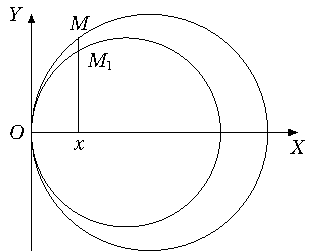
\includegraphics[scale=1]{figure/fig1-1-1.pdf}
			\caption{}\label{fig:1.1.1}
		\end{figure}
	\end{ti}
	\subsection{数列极限}

	\begin{ti}
		求 $\lim_{n \to \infty} n^{3} \left( \sin\frac{1}{n} - \frac{1}{2} \sin\frac{2}{n} \right)$.
	\end{ti}

	\begin{ti}
		求 $\lim_{n \to \infty} \left( \sqrt{n + 3\sqrt{n}} - \sqrt{n - \sqrt{n}} \right)$.
	\end{ti}

	\begin{ti}
		求 $\lim_{n \to \infty} \left[ \sqrt{n}\left( \sqrt{n+1} - \sqrt{n} \right) + \frac{1}{2} \right]^{\frac{\sqrt{n+1} + \sqrt{n}}{\sqrt{n+1} - \sqrt{n}}}$.
	\end{ti}

	\begin{ti}
		求 $\lim_{n \to \infty} n^{2} \left( a^{\frac{1}{n}} - a^{\frac{1}{n+1}} \right)$,其中 $a > 0$.
	\end{ti}

	\begin{ti}
		求 $\lim_{n \to \infty} \left( 1 + 2^{n} + 3^{n} \right)^{\frac{1}{n}}$.
	\end{ti}

	\begin{ti}
		求 $\lim_{n \to \infty} \cos\frac{x}{2}\cos\frac{x}{4}\cdots \cos\frac{x}{2^{n}}$.
	\end{ti}

	\begin{ti}
		求 $\lim_{n \to \infty} n^{2}\left( \arctan\frac{a}{n} - \arctan \frac{a}{n+1} \right)$,$a > 0$.
	\end{ti}

	\begin{ti}
		设 $\lim_{n \to \infty} \frac{n^{99}}{n^{k} - (n-1)^{k}}$ 存在且不为零,则常数 $k =$
		
		\noindent\hone{2}.
	\end{ti}

	\begin{ti}
		设数列 $\{ a_{n} \}$ 满足 $\lim_{n \to \infty}\frac{a_{n+1}}{a_{n}} = 1$,则\kuo.

		\twoch{$\{ a_{n} \}$ 有界}{$\{ a_{n} \}$ 不存在极限}{$\{ a_{n} \}$ 自某项起同号}{$\{ a_{n} \}$ 自某项起单调}
	\end{ti}

	\begin{ti}
		设数列 $\{ x_{n} \}$ 满足 $x_{n} > 0$,且 $\lim_{n \to \infty}\frac{x_{n+1}}{x_{n}} = \frac{1}{2}$,则\kuo.

		\onech{$\lim_{n\to\infty}x_{n} = 0$}{$\lim_{n\to\infty}x_{n}$ 存在,但不为零}{$\lim_{n\to\infty}x_{n}$ 不存在}{$\lim_{n\to\infty}x_{n}$ 可能存在,也可能不存在}
	\end{ti}

	\begin{ti}
		已知数列 $\{ a_{n} \}$ 单调,下列结论正确的是\kuo.
		
		\twoch{$\lim_{n \to \infty}\left( \ee^{a_{n}} - 1 \right)$ 存在}{$\lim_{n \to \infty} \frac{1}{1 + a_{n}^{2}}$ 存在}{$\lim_{n \to \infty} \sin a_{n}$ 存在}{$\lim_{n \to \infty} \frac{1}{1 - a_{n}^{2}}$ 存在}
	\end{ti}

	\begin{ti}
		设 $a_{1} = 1$,$a_{2} = 2$,$a_{n+2} = \frac{2a_{n}a_{n+1}}{a_{n} + a_{n+1}} (n=1,2,\cdots)$.
		\begin{enumerate}
			\item 求 $b_{n} = \frac{1}{a_{n+1}} - \frac{1}{a_{n}}$ 的表达式;
			\item 求 $\sum_{k=1}^{n} b_{k}$ 和 $\lim_{n \to \infty} a_{n}$.
		\end{enumerate}
	\end{ti}

	\begin{ti}
		设 $a_{1} = 3$,$a_{n+1} = a_{n}^{2} + a_{n}(n = 1,2,\cdots)$,求极限
		\[
			\lim_{n \to \infty} \left( \frac{1}{1 + a_{1}} + \frac{1}{1 + a_{2}} + \cdots + \frac{1}{1 + a_{n}} \right).
		\]
	\end{ti}
	
	\begin{ti}
		已知 $x_{1} = \frac{1}{2}$,$2 x_{n+1} + x_{n}^{2} = 1$,求 $\lim_{n \to \infty} x_{n}$.
	\end{ti}

	\begin{ti}
		设 $x_{1} = 1$,$x_{n} = 1 + \frac{1}{1 + x_{n-1}}(n = 2,3,\cdots)$. 证明 $\lim_{n \to \infty} x_{n}$ 存在,并求该极限.
	\end{ti}

	\begin{ti}
		设 $x_{1} = 1$,$x_{n+1} = \frac{x_{n} + 3}{x_{n} + 1}$,求 $\lim_{n \to \infty} x_{n}$.
	\end{ti}

	\begin{ti}
		设当 $a \leq x \leq b$ 时,$a \leq f(x) \leq b$,并设存在常数 $k$,$0 \leq k < 1$,对于 $[a,b]$ 上的任意两点 $x_{1}$ 与 $x_{2}$,都有 $|f(x_{1}) - f(x_{2})| \leq k |x_{1} - x_{2}|$. 证明:
		\begin{enumerate}
			\item 存在唯一的 $\xi \in [a,b]$ 使 $f(\xi) = \xi$;
			\item 对于任意给定的 $x_{1} \in [a,b]$,定义 $x_{n+1} = f(x_{n})$,$n = 1,2,\cdots$,则 $\lim_{n \to \infty} x_{n}$ 存在,且 $\lim_{n \to \infty} x_{n} = \xi$.
		\end{enumerate}
	\end{ti}

	\begin{ti}
		已知 $\left( 2 + \sqrt{2} \right)^{n} = A_{n} + B_{n}\sqrt{2}$,$A_{n},B_{n}$ 为整数,$n = 1,2,3,\cdots$,求 $\lim_{n\to \infty} \frac{A_{n}}{B_{n}}$.
	\end{ti}

	\begin{ti}
		设 $f(x)$ 在 $[0,+\infty)$ 上连续,满足 $0 \leq f(x) \leq x, x \in [0,+\infty)$,设 $a_{1} \geq 0$,$a_{n+1} = f(a_{n})(n = 1,2,\cdots)$,证明:
		\begin{enumerate}
			\item $\{ a_{n} \}$ 为收敛数列;
			\item 设 $\lim_{n \to \infty} a_{n} = t$,则有 $f(t) = t$;
			\item 若条件改为 $0 \leq f(x) < x,x \in (0,+\infty)$,则 $t = 0$.
		\end{enumerate}
	\end{ti}

	\begin{ti}
		\begin{enumerate}
			\item 设 $f(x) = x + \ln(2 - x)$,求 $f(x)$ 的最大值;
			\item 设 $x_{1} = \ln 2$,$x_{n} = \sum_{i=1}^{n-1} \ln(2 - x_{i}), n = 2,3,\cdots$,证明 $\lim_{n \to \infty} x_{n}$ 存在并求其极限值.
		\end{enumerate}
	\end{ti}

	\begin{ti}
		设 $x_{1} = 1$,$x_{n} = \int_{0}^{1} \min\{x,x_{n-1}\} \dd{x}, n = 2,3,\cdots$,证明 $\lim_{n \to \infty} x_{n}$ 存在并求其极限值.
	\end{ti}

	\begin{ti}
		设数列 $\{ x_{n} \}$ 满足 $0 < x_{1} < 1$,$\ln(1 + x_{n}) = \ee^{x_{n+1}} - 1(n = 1,2,\cdots)$,证明
		\begin{enumerate}
			\item 当 $0 < x < 1$ 时,$\ln(1 + x) < x < \ee^{x} - 1$;
			\item $\lim_{n \to \infty} x_{n}$ 存在,并求该极限.
		\end{enumerate}
	\end{ti}

	\begin{ti}
		\begin{enumerate}
			\item 证明方程 $x = 2\ln(1 + x)$ 在 $(0,+\infty)$ 内有唯一实根 $\xi$;
			\item 任取 $x_{1} > \xi$,定义 $x_{n+1} = 2\ln(1 + x_{n}), n = 1,2,\cdots$,证明 $\lim_{n \to \infty} x_{n} = \xi$.
		\end{enumerate}
	\end{ti}

	\begin{ti}
		\begin{enumerate}
			\item 证明方程 $\ee^{x} + x^{2n+1} = 0$ 在 $(-1,0)$ 内有唯一实根 $x_{n}, n = 0,1,2,\cdots$;
			\item 证明 $\lim_{n \to \infty} x_{n}$ 存在并求其值 $a$;
			\item 求 $\lim_{n \to \infty} n(x_{n} - a)$.
		\end{enumerate}
	\end{ti}

	\begin{ti}
		设 $F(x,y) = \frac{f(y - x)}{2x}$,$F(1,y) = \frac{y^{2}}{2} - y + 5$,$x_{0} > 0$,$x_{1} = F(x_{0},2x_{0})$,$\cdots$,$x_{n+1} = F(x_{n},2x_{n}), n = 1,2,\cdots$. 证明 $\lim_{n \to \infty} x_{n}$ 存在,并求该极限.
	\end{ti}

	\begin{ti}
		已知
		\[
			f_{n}(x) = \CC_{n}^{1} \cos x - \CC_{n}^{2} \cos^{2}x + \cdots + (-1)^{n-1} \CC_{n}^{n} \cos^{n}x.
		\]
		\begin{enumerate}
			\item 证明方程 $f_{n}(x) = \frac{1}{2}$ 在区间 $\left( 0,\frac{\uppi}{2} \right)$ 中仅有一根 $x_{n}, n = 1,2,3,\cdots$;
			\item 求 $\lim_{n \to \infty} f_{n}\left( \arccos\frac{1}{n} \right)$;
			\item 设 $x_{n} \in \left( 0,\frac{\uppi}{2} \right)$ 满足 $f_{n}(x_{n}) = \frac{1}{2}$,证明 $\lim_{n \to \infty} x_{n} = \frac{\uppi}{2}$.
		\end{enumerate}
	\end{ti}

	\begin{ti}
		\begin{enumerate}
			\item 证明:当 $x \to 0^{+}$ 时,不等式 $0 < \tan^{2}x - x^{2} < x^{4}$ 成立;
			\item 设 $x_{n} = \sum_{k=1}^{n} \tan^{2}\frac{1}{\sqrt{n+k}}$,求 $\lim_{n \to \infty}x_{n}$.
		\end{enumerate}
	\end{ti}

	\begin{ti}
		\begin{enumerate}
			\item 设 $f(x)$ 在 $(0,+\infty)$ 内可导,$f'(x) > 0, x \in (0,+\infty)$,证明 $f(x)$ 在 $(0,+\infty)$ 内单调增加;
			\item 证明 $f(x) = \left( n^{x} + 1 \right)^{-\frac{1}{x}}$ 在 $(0,+\infty)$ 内单调增加,其中 $n$ 为正整数;
			\item 设数列 $x_{n} = \sum_{k=1}^{n} \left( n^{k} + 1 \right)^{-\frac{1}{k}}$,求 $\lim_{n \to \infty} x_{n}$.
		\end{enumerate}
	\end{ti}
	\subsection{连续与间断}

	\begin{ti}
		当 $x \in \left( -\frac{1}{2},1 \right]$ 时,确定函数 $f(x) = \frac{\tan \uppi x}{|x|\left( x^{2} - 1 \right)}$ 的间断点,并判定其类型.
	\end{ti}

	\begin{ti}
		确定函数 $f(x) = \frac{x(x - 1)}{|x| x^{2} - |x|}$ 的间断点,并判定其类型.
	\end{ti}

	\begin{ti}
		设 $a > 0$,$b > 0$,$c > 0$,
		\[
			A(x) = \begin{cases}
				\left( \frac{a^{x} + b^{x}}{2} \right)^{\frac{1}{x}}, & x \ne 0,\\
				c, & x = 0.
			\end{cases}
		\]
		\begin{enumerate}
			\item 讨论 $A(x)$ 在 $x = 0$ 处的连续性;
			\item 讨论 $\lim_{x \to +\infty} A(x)$,$\lim_{x \to -\infty} A(x)$,$\lim_{x \to 0} A(x)$,$A(-1)$,$A(1)$ 五者之间的大小关系.
		\end{enumerate}
	\end{ti}

	\begin{ti}
		求 $f(x) = \frac{1}{1 - \ee^{\frac{x}{1 - x}}}$ 的连续区间、间断点,并判别间断点的类型.
	\end{ti}

	\begin{ti}
		求函数 $f(x) = \lim_{n \to \infty} \frac{x^{n+2} - x^{-n}}{x^{n} + x^{-n}}$ 的间断点并指出其类型.
	\end{ti}

	\begin{ti}
		若
		\[
			f(x) = \frac{\sqrt[3]{x}}{\lambda - \ee^{-kx}}
		\]
		在 $(-\infty,+\infty)$ 内连续,且 $\lim_{x \to -\infty} f(x) = 0$,则\kuo.
		
		\twoch{$\lambda < 0, k < 0$}{$\lambda < 0, k > 0$}{$\lambda \geq 0, k < 0$}{$\lambda \leq 0, k > 0$}
	\end{ti}

	\begin{ti}
		若
		\[
			f(x) = \begin{cases}
				\ee^{x} (\sin x + \cos x), & x > 0,\\
				2x + a, & x \leq 0
			\end{cases}
		\]
		 是 $(-\infty,+\infty)$ 内的连续函数,则 $a =$\hone{2}.
	\end{ti}

	\begin{ti}
		试讨论函数 $g(x) = \begin{cases}
			x^{\alpha} \sin\frac{1}{x}, & x > 0,\\
			\ee^{x} + \beta, & x \leq 0
		\end{cases}$ 在点 $x = 0$ 处的连续性.
	\end{ti}

	\begin{ti}
		求函数 $F(x) = \begin{cases}
			\frac{x(\uppi + 2x)}{2 \cos x}, & x \leq 0,\\
			\sin\frac{1}{x^{2} - 1}, & x > 0
		\end{cases}$ 的间断点,并判断它们的类型.
	\end{ti}

	\begin{ti}
		设 $f(x) = \lim_{n \to \infty}\frac{\ee^{\frac{1}{x}} \arctan\frac{1}{1 + x}}{x^{2} + \ee^{nx}}$,求 $f(x)$ 的间断点并判定其类型.
	\end{ti}

	\begin{ti}
		设 $f(x) = \begin{cases}
			\ee^{\frac{1}{x - 1}}, & x > 0,\\
			\ln(1 + x), & -1 < x < 0,
		\end{cases}$ 求 $f(x)$ 的间断点,并说明间断点的类型.
	\end{ti}

	\begin{ti}
		设 $f(x;t) = \left( \frac{x - 1}{t - 1} \right)^{\frac{t}{x - t}}((x - 1)(t - 1)>0, x \ne t)$,函数 $f(x)$ 由表达式
		\[
			f(x) = \lim_{t \to x}f(x;t)
		\]
		确定,求 $f(x)$ 的连续区间和间断点,并判定间断点的类型.
	\end{ti}

	\begin{ti}
		设函数 $f(x)$ 在 $[a,b]$ 上连续,$x_{1},x_{2},\cdots,x_{n},\cdots$ 是 $[a,b]$ 上的一个点列,求 $\lim_{n \to \infty} \sqrt[n]{\frac{1}{n}\sum_{k=1}^{n}\ee^{f(x_{k})}}$.
	\end{ti}

	\begin{ti}
		\begin{enumerate}
			\item 求函数 $f(x) = \lim_{n \to \infty} \sqrt[n]{1 + (2x)^{n} + x^{2n}}(x \geq 0)$ 的表达式;
			\item 讨论函数 $f(x)$ 的连续性.
		\end{enumerate}
	\end{ti}

	\begin{ti}
		已知 $f(x) = \lim_{n \to \infty} \frac{x^{2n-1} + ax^{2} + bx}{x^{2n} + 1}$ 是连续函数,求 $a,b$ 的值.
	\end{ti}

	\begin{ti}
		求函数 $f(x) = \frac{x^{3} + 1}{|x + 1|\left( x^{2} - x \right)} \sin\left( \frac{|x - 1|}{x + 2}\uppi \right)$ 的所有间断点,并判断它们的类型.
	\end{ti}
	\section{一元函数微分学}
	\subsection{一点的导数问题}

	\begin{ti}
		设 $f(x)$ 在 $x = 1$ 处可导,$f'(1) = 1$,求 $\lim_{x \to 1} \frac{f(x) - f(1)}{x^{10} - 1}$.
	\end{ti}

	\begin{ti}
		设 $f(x)$ 在 $x = 0$ 处连续,且 $\lim_{x \to 0} \left[ \frac{\ee^{f(x)} - \cos x + \sin x}{x} \right] = 0$,求 $f(0)$,并讨论 $f(x)$ 在 $x = 0$ 处是否可导?若可导,请求出 $f'(0)$.
	\end{ti}

	\begin{ti}
		函数 $f(x)$ 在 $(-\infty,+\infty)$ 内有定义,在区间 $[0,2]$ 上,$f(x) = x\left( x^{2} - 4 \right)$. 假若对任意的 $x$ 都满足 $f(x) = k f(x + 2)$,其中 $k$ 为常数.
		\begin{enumerate}
			\item 写出 $f(x)$ 在 $[-2,0)$ 上的表达式;
			\item 问 $k$ 为何值时,$f(x)$ 在 $x = 0$ 处可导?
		\end{enumerate}
	\end{ti}

	\begin{ti}
		设 $f(x)$ 在 $(-\infty,+\infty)$ 内有定义,且 $f'(0) = a(a \ne 0)$,又对任意的 $x,y \in (-\infty,+\infty)$,有
		\[
			f(x + y) = \frac{f(x) + f(y)}{1 - f(x)f(y)},
		\]
		求 $f(x)$.
	\end{ti}
	
	\begin{ti}
		设 $f(x)$ 在 $(-\infty,+\infty)$ 内有定义,且对任意的 $x,x_{1},x_{2} \in (-\infty,+\infty)$,有
		\[
			f(x_{1} + x_{2}) = f(x_{1}) \cdot f(x_{2}),f(x) = 1 + xg(x),
		\]
		其中 $\lim_{x \to 0} g(x) = 1$. 证明:$f(x)$ 在 $(-\infty,+\infty)$ 内处处可导.
	\end{ti}

	\begin{ti}
		设 $f(x)$ 定义在 $\mathbb{R}$ 上,对于任意的 $x_{1},x_{2}$,有 $|f(x_{1}) - f(x_{2})| \leq (x_{1} - x_{2})^{2}$,求证:$f(x)$ 是常值函数.
	\end{ti}

	\begin{ti}
		设 $f''(1)$ 存在,且 $\lim_{x \to 1}\frac{f(x)}{x - 1} = 0$. 记
		\[
			\varphi(x) = \int_{0}^{1} f'[1 + (x - 1)t]\dd{t}.
		\]
		求 $\varphi(x)$ 在 $x = 1$ 的某个邻域内的导数,并讨论 $\varphi'(x)$ 在 $x = 1$ 处的连续性.
	\end{ti}

	\begin{ti}
		设函数
		\[
			f(x) = \begin{cases}
				x^{3} \sin\frac{1}{x}, & x \ne 0,\\
				0, & x = 0.
			\end{cases}
		\]
		讨论 $f(x)$ 在 $x = 0$ 的可导性以及 $f'(x)$ 在 $x = 0$ 的连续性.
	\end{ti}

	\begin{ti}
		已知函数 $f(x) = \begin{cases}
			\frac{\int_{x}^{2x} \ee^{t^{2}} \dd{t}}{x}, & x \ne 0,\\
			a, & x = 0
		\end{cases}$ 在 $x = 0$ 处可导. 求
		\begin{enumerate}
			\item $a$ 的值;
			\item $f'(0)$.
		\end{enumerate}
	\end{ti}

	\begin{ti}
		若 $f(x) = \begin{cases}
			\ln\left( 1 + x^{2} \right), & x \leq 0,\\
			a \sin x + 2x, & x > 0
		\end{cases}$ 是可导函数,则 $a = $\htwo.
	\end{ti}

	\begin{ti}
		设 $f(x) = \begin{cases}
			\frac{1 - \cos x}{\sqrt{x}}, & x > 0,\\
			x^{2} g(x), & x \leq 0,
		\end{cases}$ 其中 $g(x)$ 是有界函数,则 $f(x)$ 在 $x = 0$ 处\kuo.

		\twoch{极限不存在}{极限存在,但不连续}{连续,但不可导}{可导}
	\end{ti}

	\begin{ti}
		设函数 $f(x)$ 是定义在 $(-1,1)$ 内的奇函数,且 $\lim_{x \to 0^{+}} \frac{f(x)}{x} = a \ne 0$,则 $f(x)$ 在 $x = 0$ 处的导数为\kuo.

		\fourch{$a$}{$-a$}{$0$}{不存在}
	\end{ti}

	\begin{ti}
		设函数 $f(x)$ 在 $x = 0$ 处连续,且 $\lim_{x \to 0} \frac{f\left( x^{2} \right)}{x^{2}} = 1$,则\kuo.

		\twoch{$f(0) = 0$ 且 $f_{-}'(0)$ 存在}{$f(0) = 1$ 且 $f_{-}'(0)$ 存在}{$f(0) = 0$ 且 $f_{+}'(0)$ 存在}{$f(0) = 1$ 且 $f_{+}'(0)$ 存在}
	\end{ti}

	\begin{ti}
		设 $g(x)$ 在 $x = 0$ 处二阶可导,且 $g(0) = g'(0) = 0$,设
		\[
			f(x) = \begin{cases}
				\frac{g(x)}{x}, & x \ne 0,\\
				0, & x = 0,
			\end{cases}
		\]
		则 $f(x)$ 在 $x = 0$ 处\kuo.

		\onech{不连续}{连续,但不可导}{可导,但导函数不连续}{可导且导函数连续}
	\end{ti}

	\begin{ti}
		若
		\[
			f(x) = \ee^{10x} x (x + 1) (x + 2) \cdots (x + 10),
		\]
		则 $f'(0) = $\htwo.
	\end{ti}

	\begin{ti}
		已知 $f(x) = \frac{(x - 1) (x - 2) (x - 3) \cdots (x - 100)}{(x + 1) (x + 2) (x + 3) \cdots (x + 100)}$,求 $f'(1)$.
	\end{ti}

	\begin{ti}
		设函数 $f(x) = \left( \ee^{x} - 1 \right) \left( \ee^{2x} - 2 \right) \cdots \left( \ee^{nx} - n \right)$,其中 $n$ 为正整数,则 $f'(0) = $\kuo.

		\twoch{$(-1)^{n-1}(n - 1)!$}{$(-1)^{n}(n - 1)!$}{$(-1)^{n-1}n!$}{$(-1)^{n}n!$}
	\end{ti}

	\begin{ti}
		已知 $f(x) = \sqrt{1 + x} + \arcsin\frac{1 - x}{1 + x^{2}}$,求 $f'(1)$.
	\end{ti}

	\begin{ti}
		设 $f(x) = \sqrt{\frac{(1 + x)\sqrt{x}}{\ee^{x - 1}}} + \arcsin\frac{1 - x}{\sqrt{1 + x^{2}}}$,求 $f'(1)$.
	\end{ti}

	\begin{ti}
		设 $f(x)$ 可导,$F(x) = f(x) (1 + |\sin x|)$,若使 $F(x)$ 在 $x = 0$ 处可导,则必有\kuo.

		\twoch{$f(0) = 0$}{$f'(0) = 0$}{$f(0) + f'(0) = 0$}{$f(0) - f'(0) = 0$}
	\end{ti}

	\begin{ti}
		设 $f(x)$ 在 $x = a$ 处连续,$F(x) = f(x) |x - a|$,则 $f(a) = 0$ 是 $F(x)$ 在 $x = a$ 处可导的\kuo.

		\onech{充要条件}{充分非必要条件}{必要非充分条件}{既非充分又非必要条件}
	\end{ti}

	\begin{ti}
		函数 $F(x) = \left( x^{2} - x - 2 \right)\left| x^{3} - x \right|$ 不可导的点的个数为\kuo.
		
		\fourch{$1$}{$2$}{$3$}{$4$}
	\end{ti}

	\begin{ti}
		设 $f(x) = \left| \begin{smallmatrix}
			1 & x - 1 & 2 x - 1\\
			1 & x - 2 & 3 x - 2\\
			1 & x - 3 & 4 x - 3
		\end{smallmatrix} \right|$,证明:存在 $\xi \in (0,1)$,使得 $f'(\xi) = 0$.
	\end{ti}
	\subsection{导数计算}
	
	\begin{ti}
		设 $y = \ee^{x^{2}}$,求 $\frac{\dd{y}}{\dd{x}}, \frac{\dd{y}}{\dd{\left( x^{2} \right)}}, \frac{\dd^{2}{y}}{\dd{x^{2}}}$
	\end{ti}

	\begin{ti}
		设 $f(x) = (\cos x - 4)\sin x + 3x$.
		\begin{enumerate}
			\item 求 $\frac{\dd{f(x)}}{\dd{\left( x^{2} \right)}}$;
			\item 当 $x \to 0$ 时,$f(x)$ 为 $x$ 的几阶无穷小?
		\end{enumerate}
	\end{ti}

	\begin{ti}
		设 $f'(0) = 1$,$f''(0) = 1$,求证:在 $x = 0$ 处,有
		\[
			\frac{\dd^{2}}{\dd{x^{2}}} f\left( x^{2} \right) = \frac{\dd^{2}}{\dd{x^{2}}} f^{2}(x).
		\]
	\end{ti}

	\begin{ti}
		设 $f(x)$ 为可微函数,证明:若 $x = 1$ 时,有 $\frac{\dd{f\left( x^{2} \right)}}{\dd{x}} = \frac{\dd{f^{2}(x)}}{\dd{x}}$,则必有 $f'(1) = 0$ 或 $f(1) = 1$.
	\end{ti}
	
	\begin{ti}
		设函数 $f(x) = x^{3} + 2x - 4$,$g(x) = f[f(x)]$,则 $g'(0) =$\hone{2}.
	\end{ti}

	\begin{ti}
		设 $y = f\left( \frac{3x - 2}{3x + 2} \right)$ 且 $f'(x) = \arctan x^{2}$,求 $\left. \frac{\dd{y}}{\dd{x}} \right|_{x = 0}$.
	\end{ti}

	\begin{ti}
		设 $f(x) = \begin{cases}
			x^{3x}, & x > 0,\\
			x + 1, & x \leq 0,
		\end{cases}$ 求 $f''(x)$.
	\end{ti}

	\begin{ti}
		设 $f(x)$ 在 $(-\infty,+\infty)$ 内连续且大于 $0$,
		\[
			g(x) = \begin{cases}
				\frac{\int_{0}^{x} tf(t) \dd{t}}{\int_{0}^{x} f(t) \dd{t}}, & x \ne 0,\\
				0, & x = 0.
			\end{cases}
		\]
		\begin{enumerate}
			\item 求 $g'(x)$;
			\item 证明:$g'(x)$ 在 $(-\infty,+\infty)$ 内连续.
		\end{enumerate}
	\end{ti}

	\begin{ti}
		已知可微函数 $y = y(x)$ 由方程 $y = - y\ee^{x} + 2\ee^{y} \sin x - 7x$ 所确定,求 $y''(0)$.
	\end{ti}

	\begin{ti}
		设函数 $y = y(x)$ 由参数方程 $\begin{cases}
			x = 1 + t^{2},\\
			y = \cos t
		\end{cases}$ 所确定,求:
		\begin{enumerate}
			\item $\frac{\dd{y}}{\dd{x}}$ 和 $\frac{\dd^{2}y}{\dd{x^{2}}}$;
			\item $\lim_{x \to 1^{+}} \frac{\dd{y}}{\dd{x}}$ 和 $\lim_{x \to 1^{+}} \frac{\dd^{2}y}{\dd{x^{2}}}$.
		\end{enumerate}
	\end{ti}

	\begin{ti}
		设函数 $f(x)$ 二阶可导,$f'(0) = 1$,$f''(0) = 2$,且 $\begin{cases}
			x = f(t) - \uppi,\\
			y = f\left( \ee^{3t} - 1 \right),
		\end{cases}$ 求 $\left. \frac{\dd{y}}{\dd{x}} \right|_{t = 0}$,$\left. \frac{\dd^{2}y}{\dd{x^{2}}} \right|_{t = 0}$.
	\end{ti}

	\begin{ti}
		设函数 $y = f(x)$ 是由
		\[
			\begin{cases}
				x^{x} + tx - t^{2} = 0,\\
				\arctan(ty) = \ln\left( 1 + t^{2}y^{2} \right)
			\end{cases}
		\]
		确定,求 $\frac{\dd{y}}{\dd{x}}$.
	\end{ti}

	\begin{ti}
		设 $u = f\left[ \varphi(x) + y^{2} \right]$,其中 $y = y(x)$ 由方程 $y + \ee^{y} = x$ 确定,且 $f(x), \varphi(x)$ 均有二阶导数,求 $\frac{\dd{u}}{\dd{x}}$ 和 $\frac{\dd^{2}u}{\dd{x^{2}}}$.
	\end{ti}

	\begin{ti}
		设 $y = x^{3} + 3x + 1$,则 $\left. \frac{\dd{x}}{\dd{y}} \right|_{y = 1}=$\hone{2}.
	\end{ti}

	\begin{ti}
		设 $x = f(y)$ 是函数 $y = x + \ln x$ 的反函数,求 $\frac{\dd^{2}f}{\dd{y^{2}}}$.
	\end{ti}

	\begin{ti}
		设 $y = f(x)$ 与 $x = g(y)$ 互为反函数,$y = f(x)$ 可导,且 $f'(x) \ne 0$,$f(3) = 5$,
		\[
			h(x) = f\left[ \frac{1}{3} g^{2}\left( x^{2} + 3x + 1 \right) \right],
		\]
		求 $h'(1)$.
	\end{ti}

	\begin{ti}
		设 $y = \left[ (1 + x)(3 + x)^{9} \right]^{\frac{1}{2}} (2 + x)^{4}$,求 $y'(0)$.
	\end{ti}

	\begin{ti}
		已知 $u = g(\sin y)$,其中 $g'(v)$ 存在,$y = f(x)$ 由参数方程
		\[
			\begin{cases}
				x = a \cos t,\\
				y = b \sin t
			\end{cases}
			\left( 0 < t < \frac{\uppi}{2}, a \ne 0 \right)
		\]
		所确定,求 $\dd{u}$.
	\end{ti}

	\begin{ti}
		设 $x = f(t) \cos t - f'(t) \sin t$,$y = f(t) \sin t + f'(t) \cos t$,$f''(t)$ 存在,试证:
		\[
			(\dd{x})^{2} + (\dd{y})^{2} = \left[ f(t) + f''(t) \right]^{2} (\dd{t})^{2}.
		\]
	\end{ti}

	\begin{ti}
		设 $f(x) = x \ee^{-x}$,则 $f^{(n)}(x) = $\kuo.
		
		\twoch{$(-1)^{n} (1 + n) x \ee^{-x}$}{$(-1)^{n} (1 - n) x \ee^{-x}$}{$(-1)^{n} (x + n) \ee^{-x}$}{$(-1)^{n} (x - n) \ee^{-x}$}
	\end{ti}

	\begin{ti}
		若 $f(x) = x^{5} \ee^{6x}$,则 $f^{(2019)}(0) = $\hone{4}.
	\end{ti}

	\begin{ti}
		设 $f(x) = \frac{x}{1 - 2x^{4}}$,则 $f^{(101)}(0) = $\hone{4}.
	\end{ti}

	\begin{ti}
		设 $f(x) = \ee^{x} \sin x$,则 $f^{(7)}(x) = $\hone{4}.
	\end{ti}

	\begin{ti}
		设 $f(x) = \lim_{n \to \infty} x \cos 2x \cos \frac{x}{2} \cos \frac{x}{4} \cdots \cos \frac{x}{2^{n}}(x > 0)$.
		\begin{enumerate}
			\item 求证 $f(x) = \cos 2x \sin x$;
			\item 求 $f^{(20)}(x)$.
		\end{enumerate}
	\end{ti}

	\begin{ti}
		设 $f(x) = \left( x^{2} - 3x + 2 \right)^{n} \cos \frac{\uppi x^{2}}{16}$,求 $f^{(n)}(2)$.
	\end{ti}

	\begin{ti}
		设 $y = \arcsin x$.
		\begin{enumerate}
			\item 证明其满足方程 $\left( 1 - x^{2} \right) y^{(n+2)} - (2n + 1) x y^{(n+1)} - n^{2} y^{(n)} = 0 (n \geq 0)$;
			\item 求 $\left. y^{(n)} \right|_{x = 0}$.
		\end{enumerate}
	\end{ti}

	\begin{ti}
		设 $f(x) = g'(x)$,
		\[
			g(x) = \begin{cases}
				\frac{\ee^{x} - 1}{x}, & x \ne 0,\\
				1, & x = 0,
			\end{cases}
		\]
		求 $f^{(n)}(0)$.
	\end{ti}
	\subsection{导数应用}

	\begin{ti}
		曲线 $\begin{cases}
			x = \ee^{t} \sin 2t,\\
			y = \ee^{t} \cos t
		\end{cases}$ 在点 $t = 0$ 处的切线方程为\htwo.
	\end{ti}

	\begin{ti}
		若曲线 $C: y = f(x)$ 由方程
		\[
			2x - y = 2\arctan(y - x)
		\]
		确定,则曲线 $C$ 在点 $\left( 1 + \frac{\uppi}{2}, 2 + \frac{\uppi}{2} \right)$ 处的切线方程是 $y = $\htwo.
	\end{ti}

	\begin{ti}
		曲线 $r = \cos 2 \theta$ 在 $\theta = \frac{\uppi}{4}$ 处的切线方程为\htwo.
	\end{ti}

	\begin{ti}
		已知曲线的极坐标方程 $r = 1 - \cos \theta$,求曲线上对应于 $\theta = \frac{\uppi}{6}$ 处的切线与法线的直角坐标方程.
	\end{ti}

	\begin{ti}
		已知两曲线由 $y = f(x)$ 与 $xy + \ee^{x + y} = 1$ 所确定,且在点 $(0,0)$ 处的切线相同,写出此切线方程,并求极限 $\lim_{n \to \infty} n f\left( \frac{2}{n} \right)$.
	\end{ti}

	\begin{ti}
		设 $y = f(x)$ 由参数方程 $\begin{cases}
			x = 1 + t^{2},\\
			y = \cos t
		\end{cases}$ 所确定,求曲线 $y = y(x)$ 在 $t = \frac{\uppi}{2}$ 对应点处的切线方程.
	\end{ti}

	\begin{ti}
		设周期函数 $f(x)$ 在 $(-\infty,+\infty)$ 内可导,周期为 $4$,又 $\lim_{x \to 0} \frac{f(1) - f(1 - x)}{2x} = -1$,则曲线 $y = f(x)$ 在点 $(5,f(5))$ 处的切线斜率为\kuo.
		
		\fourch{$\frac{1}{2}$}{$0$}{$-1$}{$-2$}
	\end{ti}

	\begin{ti}
		设曲线 $f(x) = x^{n}$ 在点 $(1,1)$ 处的切线与 $x$ 轴的交点为 $(x_{n},0),n = 1,2,\cdots$,求 $\lim_{n \to \infty} f(x_{n})$.
	\end{ti}

	\begin{ti}
		曲线 $\left( 2 - x^{n^{2}} \right) y = 1$ 在点 $(1,1)$ 处的切线与 $x$ 轴的交点为 $(x_{n},0),n = 1,2,\cdots$,则 $\lim_{n \to \infty} x_{n}^{\frac{n^{2}}{2}} = $\htwo.
	\end{ti}

	\begin{ti}
		设 $y = \tan^{n}x$ 在 $x = \frac{\uppi}{4}$ 处的切线在 $x$ 轴上的截距为 $x_{n}$,试求 $\lim_{n \to \infty} y(x_{n})$.
	\end{ti}

	\begin{ti}
		已知 $f(x)$ 是周期为 $5$ 的连续函数,它在 $x = 0$ 的某邻域内满足关系式
		\[
			f(1 + \sin x) - 3 f(1 - \sin x) = 8x + \alpha(x),
		\]
		其中 $\alpha(x)$ 是当 $x \to 0$ 时比 $x$ 高阶的无穷小,且 $f(x)$ 在 $x = 1$ 处可导,求 $y = f(x)$ 在点 $(6,f(6))$ 处的切线方程.
	\end{ti}

	\begin{ti}
		在左半平面 $(x < 0)$ 上,求曲线 $y = \frac{1}{x}$ 和 $y = x^{2}$ 的公切线.
	\end{ti}

	\begin{ti}
		求双曲线 $y_{1} = \frac{1}{x}$ 与抛物线 $y_{2} = \sqrt{x}$ 的交角.
	\end{ti}

	\begin{ti}
		设函数 $f(x)$ 在 $x = 2$ 处可微,且满足
		\[
			2f(2 + x) + f(2 - x) = 3 + 2x + o(x),
		\]
		这里 $o(x)$ 表示比 $x$ 高阶的无穷小(当 $x \to 0$ 时),试求微分 $\left. \dd{f(x)} \right|_{x = 2}$,并求曲线 $y = f(x)$ 在点 $(2,f(2))$ 处的切线方程.
	\end{ti}

	\begin{ti}
		若函数 $f(x) = a \sin x + \frac{1}{3} \sin 3x$ 在 $x = \frac{\uppi}{3}$ 处取得极值,则 $a = $\htwo.
	\end{ti}

	\begin{ti}
		若 $f(x)$ 在 $x_{0}$ 点至少二阶可导,且
		\[
			\lim_{x \to x_{0}} \frac{f(x) - f(x_{0})}{(x - x_{0})^{2}} = -1,
		\]
		则函数 $f(x)$ 在 $x = x_{0}$ 处\kuo.
		
		\twoch{取得极大值}{取得极小值}{无极值}{不一定有极值}
	\end{ti}

	\begin{ti}
		设 $f(x)$ 在 $x = 0$ 的某邻域内连续且在 $x = 0$ 处存在二阶导数 $f''(0)$. 又设
		\[
			\lim_{x \to 0} \frac{\int_{0}^{x} t f(x - t) \dd{t}}{x^{4}} = a(\text{常数}\  a > 0),
		\]
		则\kuo.
		
		\onech{$x = 0$ 不是 $f(x)$ 的驻点}{$x = 0$ 是 $f(x)$ 的驻点,但不是 $f(x)$ 的极值点}{$x = 0$ 是 $f(x)$ 的极小值点}{$x = 0$ 是 $f(x)$ 的极大值点}
	\end{ti}

	\begin{ti}
		设函数 $y = y(x)$ 是由方程 $\begin{cases}
			x = 2t + |t|,\\
			y = 5t^{2} + 4t|t|
		\end{cases}$ 所确定. 在 $t = 0$ 处,函数 $y = y(x)$ \kuo.
		
		\onech{导数存在,但 $y'(0) \ne 0$}{导数 $y'(0) = 0$,但不是极值点}{是极小值点}{是极大值点}
	\end{ti}

	\begin{ti}
		已知 $f'(-x) = x\left[ f'(x) + 1 \right]$,求 $f(x)$ 的极值点,并说明是极大值点还是极小值点.
	\end{ti}

	\begin{ti}
		设函数 $f(x)$ 可导,且满足 $xf'(x) = f'(-x) + 1$,$f(0) = 0$,求:
		\begin{enumerate}
			\item $f'(x)$;
			\item 函数 $f(x)$ 的极值.
		\end{enumerate}
	\end{ti}

	\begin{ti}
		求函数 $f(x) = |x| \ee^{-|x - 1|}$ 的极值.
	\end{ti}

	\begin{ti}
		求函数 $f(x) = \begin{cases}
			x^{2x}, & x > 0,\\
			x + 2, & x \leq 0
		\end{cases}$ 的单调区间和极值.
	\end{ti}

	\begin{ti}
		设 $f(x) = f(-x)$,且在 $(0,+\infty)$ 内二阶可导,又 $f'(x) > 0$,$f''(x) < 0$,则 $f(x)$ 在 $(-\infty,0)$ 内的单调性和图形的凹凸性是\kuo.
		
		\twoch{单调增加,凸}{单调减少,凸}{单调增加,凹}{单调减少,凹}
	\end{ti}

	\begin{ti}
		设函数 $y = y(x)$ 由参数方程
		\[
			\begin{cases}
				x = t^{3} + 9t,\\
				y = t^{2} - 2t
			\end{cases}
		\]
		确定,求曲线 $y = y(x)$ 的凹区间.
	\end{ti}

	\begin{ti}
		设函数 $f(x)$ 在 $(-\infty,+\infty)$ 内连续,其一阶导函数 $f'(x)$ 的图形如图~\ref{fig:1.2.1} 所示,并设在 $f'(x)$ 存在处 $f''(x)$ 亦存在,则函数 $f(x)$ 及曲线 $y = f(x)$\kuo.
		
		\onech{只有 $1$ 个极大值点与 $1$ 个拐点}{有 $1$ 个极小值点,$1$ 个极大值点与 $1$ 个拐点}{有 $1$ 个极小值点,$1$ 个极大值点与 $2$ 个拐点}{有 $1$ 个极小值点,$1$ 个极大值点与 $3$ 个拐点}
		\begin{figure}[htbp]
			\centering
			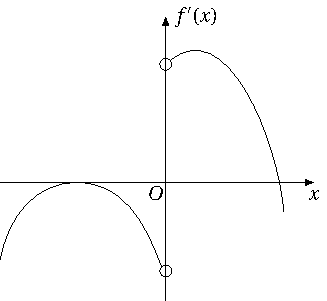
\includegraphics[scale=1]{figure/fig1-2-1.pdf}
			\caption{}\label{fig:1.2.1}
		\end{figure}
	\end{ti}

	\begin{ti}
		当 $x > 0$ 时,曲线 $y = x \sin\frac{1}{x}$ \kuo.
		
		\onech{有且仅有水平渐近线}{有且仅有铅直渐近线}{既有水平渐近线,也有铅直渐近线}{既无水平渐近线,也无铅直渐近线}
	\end{ti}

	\begin{ti}
		曲线 $y = \ln\left( \ee - \frac{1}{x} \right)$ 的全部渐近线为\htwo
		
		\noindent\htwo.
	\end{ti}

	\begin{ti}
		曲线 $y = \ee^{\frac{1}{x^{2}}} \arctan \frac{x^{2} + x + 1}{(x - 1)(x + 2)}$ 的渐近线有\kuo.
		
		\fourch{$1$ 条}{$2$ 条}{$3$ 条}{$4$ 条}
	\end{ti}

	\begin{ti}
		求 $y = \sqrt{4x^{2} + x} \ln\left( 2 + \frac{1}{x} \right)$ 的全部渐近线.
	\end{ti}

	\begin{ti}
		函数 $y = (x - 1)^{2} (x - 2)^{2} (-3 \leq x \leq 4)$ 的值域是
		
		\noindent\htwo.
	\end{ti}

	\begin{ti}
		设正值函数 $f(x)$ 在 $(1,+\infty)$ 内连续,求函数
		\[
			F(x) = \int_{1}^{x} \left[ \left( \frac{2}{x} + \ln x \right) - \left( \frac{2}{t} + \ln t \right) \right] f(t) \dd{t}
		\]
		的最小值点.
	\end{ti}

	\begin{ti}
		函数 $y = x^{x}$ 在区间 $\left[ \frac{1}{\ee},+\infty \right)$ 上\kuo.
		
		\onech{不存在最大值和最小值}{最大值是 $\ee^{\frac{1}{\ee}}$}{最大值是 $\left( \frac{1}{\ee} \right)^{\frac{1}{\ee}}$}{最小值是 $\left( \frac{1}{\ee} \right)^{\frac{1}{\ee}}$}
	\end{ti}

	\begin{ti}
		求函数 $f_{n}(x) = x^{n} \ee^{- n^{2} x}(n = 2,3,\cdots)$ 在 $[0,+\infty)$ 内的最值,并求极限 $\lim_{n \to \infty} f_{n}(x), x \geq 0$.
	\end{ti}

	\begin{ti}
		设 $f(x) = \begin{cases}
			\lim_{n \to \infty} \frac{1}{n} \sum_{k=0}^{n-1} \cos \frac{k}{n}x, & x > 0,\\
			1, & x = 0,\\
			f(-x), & x < 0.
		\end{cases}$
		\begin{enumerate}
			\item 求 $f'(0)$;
			\item 求 $f(x)$ 在 $[-\uppi,\uppi]$ 上的最大值.
		\end{enumerate}
	\end{ti}

	\begin{ti}
		设某物体的温度 $T$ 与时间 $t$ 满足函数关系:
		\[
			T = a\left( 1 - \ee^{-kt} \right) + b,
		\]
		其中 $T$ 的单位是 \si{\degreeCelsius},$t$ 的单位是 \si{min}. 现将该物体放入 \SI{200}{\degreeCelsius} 的高温介质中.
		\begin{enumerate}
			\item 若物体的初始温度是 \SI{20}{\degreeCelsius},求 $a$ 和 $b$;
			\item 若物体温度以 \SI{2}{\degreeCelsius/min} 的速率开始上升,求 $k$.
		\end{enumerate}
	\end{ti}

	\begin{ti}
		曲线 $y = y(x)$ 可表示为 $x = t^{3} - t, y = t^{4} + t$,$t$ 为参数. 证明:
		\begin{enumerate}
			\item $y = y(x)$ 在 $t = 0$ 处为拐点;
			\item $g(x) = \sqrt{\left( \frac{\dd{x}}{\dd{t}} \right)^{2} + \left( \frac{\dd{y}}{\dd{t}} \right)^{2}}$ 在 $t = 0$ 处取得极大值.
		\end{enumerate}
	\end{ti}

	\begin{ti}
		设有曲线弧 $y = \sin x(0 < x < \uppi)$.
		\begin{enumerate}
			\item 求出曲线弧的最小曲率半径;
			\item 求与曲线弧在曲率半径最小的点处相切且具有相同曲率和凹向的抛物线的方程.
		\end{enumerate}
	\end{ti}

	\begin{ti}
		曲线 $2y^{3} - 2y^{2} + 2xy - x^{2} = 1$ 在 $(1,1)$ 处的曲率半径为\htwo.
	\end{ti}

	\begin{ti}
		$y^{2} = 4x$ 在原点处的曲率圆方程为\htwo.
	\end{ti}

	\begin{ti}
		求曲线 $y = \ln x$ 上曲率最大的点,并在该点附近用抛物线 $y = ax^{2} + bx + c$ 近似代替 $y = \ln x$,求 $a,b,c$.
	\end{ti}

	\begin{ti}
		质点 $P$ 沿抛物线 $x = y^{2}(y > 0)$ 移动,$P$ 的横坐标 $x$ 的变化速度 \SI{5}{cm/s}. 当 $x = 9$ 时,点 $P$ 到原点 $O$ 的距离变化速度为\htwo.
	\end{ti}

	\begin{ti}
		半径为 $\frac{1}{2}$ 的圆在抛物线 $x = \sqrt{y}$ 凹的一侧上滚动.
		\begin{enumerate}
			\item 求圆心 $(\xi,\eta)$ 的轨迹方程.
			\item 当圆心以速率 $V_{0}$ 匀速上升时,求圆心的横坐标 $\xi$ 的增长速度.
		\end{enumerate}
	\end{ti}

	\begin{ti}
		球的半径以 \SI{5}{cm/s} 的速度匀速增长,问球的半径为 \SI{50}{cm} 时,球的表面积和体积的增长速度各是多少?
	\end{ti}
	\subsection{中值定理、方程的根、不等式}

	\begin{ti}
		设函数 $f(x)$ 在 $[a,b]$ 上连续,在 $(a,b)$ 内可导,且 $f(a) = f(b) = 0$,求证:
		\begin{enumerate}
			\item 存在 $\xi \in (a,b)$,使 $f(\xi) + \xi f'(\xi) = 0$;
			\item 存在 $\eta \in (a,b)$,使 $\eta f(\eta) + f'(\eta) = 0$.
		\end{enumerate}
	\end{ti}

	\begin{ti}
		设函数 $f(x)$ 在 $[-2,2]$ 上二阶可导,且 $\left| f(x) \right| \leq 1$,又 $f^{2}(0) + \left[ f'(0) \right]^{2} = 4$. 试证:在 $(-2,2)$ 内至少存在一点 $\xi$,使得 $f(\xi) + f''(\xi) = 0$.
	\end{ti}

	\begin{ti}
		设函数 $f(x)$ 在 $[a,b]$ 上连续,在 $(a,b)$ 内可导且 $f(a) \ne f(b)$. 证明:存在 $\xi,\eta \in (a,b)$,使得 $\frac{f'(\xi)}{2\xi} = \frac{f'(\eta)}{b + a}$.
	\end{ti}

	\begin{ti}
		设函数 $f(x)$ 在闭区间 $[a,b]$ 上连续 $(a,b > 0)$,在 $(a,b)$ 内可导. 证明:在 $(a,b)$ 内至少存在一点 $\xi$,使等式 $\frac{1}{a - b} \left| \begin{smallmatrix}
			a & b\\
			f(a) & f(b)
		\end{smallmatrix} \right| = f(\xi) - \xi f'(\xi)$ 成立.
	\end{ti}

	\begin{ti}
		设 $f(x)$ 在闭区间 $[1,2]$ 上可导,证明:存在一点 $\xi \in (1,2)$,使
		\[
			f(2) - 2f(1) = \xi f'(\xi) - f(\xi).
		\]
	\end{ti}

	\begin{ti}
		设 $f(x), g(x)$ 在 $[a,b]$ 上二阶可导,且 $f(a) = f(b) = g(a) = 0$,证明:存在 $\xi \in (a,b)$,使 $f''(\xi) g(\xi) + 2 f'(\xi) g'(\xi) + f(\xi) g''(\xi) = 0$.
	\end{ti}

	\begin{ti}
		设 $f(x)$ 在闭区间 $[-1,1]$ 上具有三阶连续导数,且 $f(-1) = 0$,$f(1) = 1$,$f'(0) = 0$. 证明:在 $[-1,1]$ 内存在 $\xi$,使得 $f'''(\xi) = 3$.
	\end{ti}

	\begin{ti}
		设 $f(x), g(x)$ 在 $[a,b]$ 上二阶可导,$g''(x) \ne 0$,$f(a) = f(b) = g(a) = g(b) = 0$. 证明:
		\begin{enumerate}
			\item 在 $(a,b)$ 内,$g(x) \ne 0$;
			\item 在 $(a,b)$ 内至少存在一点 $\xi$,使 $\frac{f(\xi)}{g(\xi)} = \frac{f''(\xi)}{g''(\xi)}$.
		\end{enumerate}
	\end{ti}

	\begin{ti}
		$f(x)$ 在 $[a,b]$ 上连续,在 $(a,b)$ 内可导,且 $f'(x) \ne 0$. 证明:存在 $\xi, \eta \in (a,b)$,使得
		\[
			\frac{f'(\xi)}{f'(\eta)} = \frac{\ee^{b} - \ee^{a}}{b - a} \ee^{-\eta}.
		\]
	\end{ti}

	\begin{ti}
		设 $f(x)$ 在 $[0,1]$ 上可导,$f(0) = 0$,$\left| f'(x) \right| \leq \left| f(x) \right|$,则 $f(1) = $\htwo.
	\end{ti}

	\begin{ti}
		设 $f(x)$ 在 $[0,4]$ 上一阶可导且 $f'(x) \geq \frac{1}{4}$,$f(2) \geq 0$,则在下列区间上必有 $f(x) \geq \frac{1}{4}$ 成立的是\kuo.

		\fourch{$[0,1]$}{$[1,2]$}{$[2,3]$}{$[3,4]$}
	\end{ti}

	\begin{ti}
		设 $f(x)$ 二阶可导,$f''(x) < 0$,$f'(0) \leq \frac{1}{3}$,$f(0) = 0$,$f(1) = \frac{1}{2}$,并设 $0 < x_{n} < 1$,且 $x_{n+1} = f(x_{n}), n = 1,2,\cdots$.
		\begin{enumerate}
			\item 证明 $\frac{f(x)}{x}$ 在 $(0,+\infty)$ 内单调减少;
			\item 证明 $\lim_{n \to \infty} x_{n}$ 存在.
		\end{enumerate}
	\end{ti}

	\begin{ti}
		设 $\xi_{a}$ 为函数 $f(x) = \arctan x$ 在区间 $[0,a]$ 上使用拉格朗日中值定理时的中值,求 $\lim_{a \to 0^{+}} \frac{\xi_{a}}{a}$.
	\end{ti}

	\begin{ti}
		设函数 $f(x) = \arctan x$,若 $f(x) = f'(\xi) \sin x$,求极限 $\lim_{x \to 0} \frac{\xi^{2}}{x^{2}}$.
	\end{ti}

	\begin{ti}
		设函数 $f(x)$ 在闭区间 $[a,b]$ 上连续,在开区间 $(a,b)$ 内可导,$f'(x) \ne 0$,且 $f(a) = 0$,$f(b) = 2$. 证明在开区间 $(a,b)$ 内存在两个不同的点 $\xi,\eta$,使
		\[
			f'(\eta) \left[ f(\xi) + \xi f'(\xi) \right] = f'(\xi) \left[ b f'(\eta) - 1 \right].
		\]
	\end{ti}

	\begin{ti}
		讨论常数 $a$ 的值,确定曲线 $y = a \ee^{x}$ 与 $y = 1 + x$ 的公共点的个数.
	\end{ti}

	\begin{ti}
		讨论方程 $2x^{3} - 9x^{2} + 12x - a = 0$ 实根的情况.
	\end{ti}

	\begin{ti}
		讨论方程 $a x \ee^{x} + b = 0 (a > 0)$ 实根的情况.
	\end{ti}

	\begin{ti}
		证明:方程 $x^{\alpha} = \ln x (\alpha < 0)$ 在 $(0,+\infty)$ 内有且仅有一个实根.
	\end{ti}

	\begin{ti}
		设 $f(x)$ 可导,证明:$f(x)$ 的两个零点之间一定有 $f(x) + f'(x)$ 的零点.
	\end{ti}

	\begin{ti}
		设 $F(x) = \int_{-1}^{1} |x - t| \ee^{-t^{2}} \dd{t} - \frac{1}{2} \left( \ee^{-1} + 1 \right)$,讨论 $F(x)$ 在区间 $[-1,1]$ 上的零点个数.
	\end{ti}

	\begin{ti}
		证明:当 $x \geq 1$ 时,$\arctan x - \frac{1}{2} \arccos \frac{2x}{1 + x^{2}} \equiv \frac{\uppi}{4}$.
	\end{ti}

	\begin{ti}
		设 $\lim_{x \to 0} \frac{f(x)}{x} = 1$,且 $f''(x) > 0$. 证明:$f(x) \geq x$.
	\end{ti}

	\begin{ti}
		证明:当 $0 < a < b < \uppi$ 时,
		\[
			b \sin b + 2 \cos b + \uppi b > a \sin a + 2 \cos a + \uppi a.
		\]
	\end{ti}

	\begin{ti}
		设 $b > a > \ee$,证明:$a^{b} > b^{a}$.
	\end{ti}

	\begin{ti}
		设一质点在单位时间内由点 $A$ 从静止开始做直线运动至点 $B$ 停止,$A,B$ 两点间距离为 $1$,证明:该质点在 $(0,1)$ 内总有一时刻的加速度的绝对值不小于 $4$.
	\end{ti}

	\begin{ti}
		在区间 $[0,a]$ 上 $\left| f''(x) \right| \leq M$,且 $f(x)$ 在 $(0,a)$ 内取得最大值. 求证:$\left| f'(0) \right| + \left| f'(a) \right| \leq Ma$.
	\end{ti}

	\begin{ti}
		设 $x \in (0,1)$,证明下面不等式
		\begin{enumerate}
			\item $(1 + x) \ln^{2}(1 + x) < x^{2}$;
			\item $\frac{1}{\ln 2} - 1 < \frac{1}{\ln(1 + x)} - \frac{1}{x} < \frac{1}{2}$.
		\end{enumerate}
	\end{ti}

	\begin{ti}
		证明:$\cos \sqrt{2} x \leq - x^{2} + \sqrt{1 + x^{4}}$,其中 $x \in \bigl( 0, \frac{\sqrt{2}\uppi}{4} \bigr)$.
	\end{ti}

	\begin{ti}
		设 $f(x)$ 在 $[a,b]$ 上二阶可导,且 $f'(a) = f'(b) = 0$,证明存在 $\xi \in (a,b)$,使
		\[
			\left| f''(\xi) \right| \geq \frac{4}{(b - a)^{2}} \left| f(b) - f(a) \right|.
		\]
	\end{ti}

	\begin{ti}
		已知 $f(x)$ 二阶可导,且 $f(x) > 0$,$f(x) f''(x) - \bigl[ f'(x) \bigr]^{2} \geq 0 (x \in \mathbb{R})$.
		\begin{enumerate}
			\item 证明 $f(x_{1}) f(x_{2}) \geq f^{2}\left( \frac{x_{1} + x_{2}}{2} \right)(x_{1}, x_{2} \in \mathbb{R})$;
			\item 若 $f(0) = 1$,证明 $f(x) \geq \ee^{f'(0) x} (x \in \mathbb{R})$.
		\end{enumerate}
	\end{ti}

	\begin{ti}
		设 $f(x)$ 在 $[a,b]$ 上具有二阶导数,且 $f''(x) > 0$,证明:
		\[
			f\left( \frac{a + b}{2} \right) < \frac{1}{b - a} \int_{a}^{b} f(t) \dd{t} < \frac{1}{2} \left[ f(a) + f(b) \right].
		\]
	\end{ti}

	\begin{ti}
		证明:$\ee^{x} + \ee^{-x} \geq 2x^{2} + 2 \cos x, -\infty < x < +\infty$.
	\end{ti}

	\begin{ti}
		设 $f(x)$ 在区间 $[0,+\infty)$ 内具有二阶导数,且 $\bigl|f(x)\bigr| \leq 1, 0 < \bigl| f''(x) \bigr| \leq 2 (0 \leq x < +\infty)$. 证明:$\bigl| f'(x) \bigr| \leq 2\sqrt{2}$.
	\end{ti}

	\begin{ti}
		若用 $\frac{2(x - 1)}{x + 1}$ 来近似 $\ln x$,证明当 $x \in [1,2]$ 时,其误差不超过 $\frac{1}{12} (x - 1)^{3}$.
	\end{ti}
	\section{一元函数积分学}
	\subsection{概念与性质}

	\begin{ti}
		设 $f(x)$ 为连续函数,$F(x) = \int_{0}^{x} f(t) \dd{t}$. 试证明:
		\begin{enumerate}
			\item $F(x)$ 的奇偶性正好与 $f(x)$ 的奇偶性相反;
			\item 若 $f(x)$ 为奇函数,则 $f(x)$ 的一切原函数均为偶函数; 若 $f(x)$ 为偶函数,则有且仅有一个原函数为奇函数.
		\end{enumerate}
	\end{ti}

	\begin{ti}
		设 $f(x)$ 在 $(-\infty,+\infty)$ 内连续,以 $T$ 为周期,证明:
		\begin{enumerate}
			\item $\int_{a}^{a + T} f(x) \dd{x} = \int_{0}^{T} f(x) \dd{x}$ ($a$ 为任意实数);
			\item $\int_{0}^{x} f(t) \dd{t}$ 以 $T$ 为周期 $\Longleftrightarrow$ $\int_{0}^{T} f(x) \dd{x} = 0$;
			\item $\int f(x) \dd{x}$ ($f(x)$ 的全体原函数) 周期为 $T$ $\Longleftrightarrow$ $\int_{0}^{T} f(x) \dd{x} = 0$.
		\end{enumerate}
	\end{ti}

	\begin{ti}
		设 $f(x)$ 连续,则在下列变上限积分中,必为偶函数的是\kuo.

		\twoch{$\int_{0}^{x} t \bigl[ f(t) + f(-t) \bigr] \dd{t}$}{$\int_{0}^{x} t \bigl[ f(t) - f(-t) \bigr] \dd{t}$}{$\int_{0}^{x} f\left( t^{2} \right) \dd{t}$}{$\int_{0}^{x} f^{2}(t) \dd{t}$}
	\end{ti}

	\begin{ti}
		设 $F(x) = \int_{x}^{x + 2\uppi} \ee^{\sin t} \dd{t}$,则 $F(x)$ \kuo.

		\twoch{为正常数}{为负常数}{恒为零}{不为常数}
	\end{ti}

	\begin{ti}
		设 $f(x)$ 是以 $l$ 为周期的周期函数,则
		\[
			\int_{a + kl}^{a + (k + 1)l} f(x) \dd{x}
		\]
		的值\kuo.

		\twoch{仅与 $a$ 有关}{仅与 $a$ 无关}{与 $a$ 及 $k$ 都无关}{与 $a$ 及 $k$ 都有关}
	\end{ti}

	\begin{ti}
		设 $f(x)$ 是以 $T$ 为周期的可微函数,则下列函数中以 $T$ 为周期的函数是\kuo.

		\twoch{$\int_{a}^{x} f(t) \dd{t}$}{$\int_{a}^{x} f\bigl( t^{2} \bigr) \dd{t}$}{$\int_{a}^{x} f'\bigl( t^{2} \bigr) \dd{t}$}{$\int_{a}^{x} f(t) f'(t) \dd{t}$}
	\end{ti}

	\begin{ti}
		设 $f(x)$ 是以 $2$ 为周期的连续函数,$G(x) = 2 \int_{0}^{x} f(t) \dd{t} - x \int_{0}^{2} f(t) \dd{t}$,则\kuo.

		\onech{$G(x)$ 是以 $2$ 为周期的周期函数,$G'(x)$ 也是以 $2$ 为周期的周期函数}{$G(x)$ 是以 $2$ 为周期的周期函数,$G'(x)$ 不是以 $2$ 为周期的周期函数}{$G(x)$ 不是以 $2$ 为周期的周期函数,$G'(x)$ 是以 $2$ 为周期的周期函数}{$G(x)$ 不是以 $2$ 为周期的周期函数,$G'(x)$ 也不是以 $2$ 为周期的周期函数}
	\end{ti}

	\begin{ti}
		设 $f(x)$ 可导,且
		\[
			f(x) = x + x \int_{0}^{1} f(x) \dd{x} + x^{2} \lim_{x \to 0} \frac{f(x)}{x},
		\]
		求 $f(x)$.
	\end{ti}

	\begin{ti}
		已知 $f(x)$ 在 $[-1,1]$ 上连续,
		\[
			f(x) = 3x - \sqrt{1 - x^{2}} \int_{0}^{1} f^{2}(x) \dd{x},
		\]
		求 $f(x)$.
	\end{ti}
	\subsection{一元积分比大小}
	
	\begin{ti}
		设 $I_{k} = \int_{0}^{k \uppi} \ee^{x^{2}} \sin x \dd{x} (k = 1,2,3)$,则有\kuo.

		\twoch{$I_{1} < I_{2} < I_{3}$}{$I_{3} < I_{2} < I_{1}$}{$I_{2} < I_{3} < I_{1}$}{$I_{2} < I_{1} < I_{3}$}
	\end{ti}

	\begin{ti}
		设 $N = \int_{-a}^{a} x^{2} \sin^{3}x \dd{x}$,$P = \int_{-a}^{a} \bigl( x^{3} \ee^{x^{2}} - 1 \bigr) \dd{x}$,$Q = \int_{-a}^{a} \cos^{2} x^{3} \dd{x}$,$a \geq 0$,则\kuo.

		\twoch{$N \leq P \leq Q$}{$N \leq Q \leq P$}{$Q \leq P \leq N$}{$P \leq N \leq Q$}
	\end{ti}

	\begin{ti}
		设
		\begin{align*}
			M &= \int_{-\frac{\uppi}{2}}^{\frac{\uppi}{2}} \frac{\sin x}{1 + x^{2}} \cos^{6}x \dd{x},\\
			N &= \int_{-\frac{\uppi}{2}}^{\frac{\uppi}{2}} \bigl( \sin^{3}x + \cos^{6}x \bigr) \dd{x},\\
			P &= \int_{-\frac{\uppi}{2}}^{\frac{\uppi}{2}} \bigl( x^{2} \sin^{3}x - \cos^{6}x \bigr) \dd{x},
		\end{align*}
		则\kuo.

		\twoch{$N < P < M$}{$M < P < N$}{$N < M < P$}{$P < M < N$}
	\end{ti}

	\begin{ti}
		设常数 $\alpha > 0$,积分
		\begin{align*}
			I_{1} &= \int_{0}^{\frac{\uppi}{2}} \frac{\cos x}{1 + x^{\alpha}} \dd{x},\\
			I_{2} &= \int_{0}^{\frac{\uppi}{2}} \frac{\sin x}{1 + x^{\alpha}} \dd{x},
		\end{align*}
		则\kuo.

		\onech{$I_{1} > I_{2}$}{$I_{1} < I_{2}$}{$I_{1} = I_{2}$}{$I_{1}$ 与 $I_{2}$ 的大小与 $\alpha$ 有关}
	\end{ti}

	\begin{ti}
		证明:$\int_{0}^{1} \frac{x \sin \frac{\uppi}{2} x}{1 + x} \dd{x} > \int_{0}^{1} \frac{x \cos \frac{\uppi}{2} x}{1 + x} \dd{x}$
	\end{ti}
	\subsection{定积分定义}

	\begin{ti}
		$\lim_{n \to \infty} \sum_{k=1}^{n} \frac{1}{\sqrt{n^{2} + kn}} = $\hone{4}.
	\end{ti}

	\begin{ti}
		已知 $f(x) = a^{x^{3}}, a > 0$ 且 $a \ne 1$. 求
		\[
			\lim_{n \to \infty} \frac{1}{n^{4}}  \ln \left[ f(1) f(2) \cdots f(n) \right].
		\]
	\end{ti}

	\begin{ti}
		$\lim_{n \to \infty} \frac{\sqrt[n]{(n + 1) (n + 2) \cdots (n + n)}}{n} = $\hone{4}.
	\end{ti}

	\begin{ti}
		$f(x) = \begin{cases}
			\ee^{-x}, & x \ne 0,\\
			\lim_{n \to \infty} 2 \sum_{k=1}^{n} \frac{n}{(n + k)^{2}}, & x = 0,
		\end{cases}$ 求 $f'(0)$.
	\end{ti}

	\begin{ti}
		$\lim_{n \to \infty} \sin \frac{\uppi}{n} \sum_{k=1}^{n} \frac{1}{2 + \cos \frac{k \uppi}{n}} = $\hone{4}.
	\end{ti}

	\begin{ti}
		$\lim_{n \to \infty} \sum_{k=1}^{n} \frac{1}{n + \frac{(k - 1)^{2} + 1}{n}} = $\hone{4}.
	\end{ti}

	\begin{ti}
		$\lim_{n \to \infty} \sum_{k=1}^{n} \frac{3^{\frac{k}{n}}}{n + \frac{1}{k}} = $\hone{4}.
	\end{ti}

	\begin{ti}
		设 $f(x) = \begin{cases}
			\lim_{n \to \infty} \sum_{k=1}^{n} \frac{|x|^{k/n}}{n + \frac{k}{n}}, & x \ne 0,\\
			0, & x = 0,
		\end{cases}$ 求 $f'(x)$.
	\end{ti}
	\subsection{分部积分法}

	\begin{ti}
		求 $\int_{0}^{1} \ln \bigl( x + \sqrt{x^{2} + 3} \bigr) \dd{x}$.
	\end{ti}

	\begin{ti}
		$\int \frac{x \ln ( x + \sqrt{1 + x^{2}} )}{\left( 1 + x^{2} \right)^{2}} \dd{x} = $\htwo.
	\end{ti}

	\begin{ti}
		$\int \frac{x \ln x}{\left( x^{2} - 1 \right)^{\frac{3}{2}}} \dd{x}$.
	\end{ti}

	\begin{ti}
		求 $\int_{-\frac{\uppi}{4}}^{\frac{\uppi}{4}} 5 \cos x \cdot \arctan \ee^{x} \dd{x}$.
	\end{ti}

	\begin{ti}
		求 $\int x \arctan x \dd{x}$.
	\end{ti}

	\begin{ti}
		求 $\int_{0}^{+\infty} \frac{x \ee^{-3x}}{\left( 1 + \ee^{-3x} \right)^{2}} \dd{x}$.
	\end{ti}

	\begin{ti}
		求 $\int_{0}^{1} x \ln (1 - x) \dd{x}$.
	\end{ti}

	\begin{ti}
		设 $f\bigl( \sin^{2}x \bigr) = \frac{x}{\sin x}$,求 $\int \frac{\sqrt{x}}{\sqrt{1 - x}} f(x) \dd{x}$.
	\end{ti}

	\begin{ti}
		已知 $f(x) = \frac{\ee^{x} + \ee^{-x}}{2}$,求 $\int \Bigl[ \frac{f'(x)}{f(x)} + \frac{f(x)}{f'(x)} \Bigr] \dd{x}$.
	\end{ti}

	\begin{ti}
		已知 $\int_{0}^{1} f(x) \dd{x} = 1$,$f(1) = 0$,则 $\int_{0}^{1} x f'(x) \dd{x} = $
		
		\noindent\htwo.
	\end{ti}

	\begin{ti}
		已知 $f(x)$ 的一个原函数为 $(1 + \sin x) \ln x$,求 $\int x f'(x) \dd{x}$.
	\end{ti}

	\begin{ti}
		设 $\frac{\ln x}{x}$ 是 $f(x)$ 的一个原函数,则 $\int_{1}^{\ee} x f'(x) \dd{x} = $
		
		\noindent\htwo.
	\end{ti}

	\begin{ti}
		设 $f(x)$ 有一个原函数 $\frac{\sin x}{x}$,则 $\int_{\frac{\uppi}{2}}^{\uppi} x^{3} f'(x) \dd{x} = $
		
		\noindent\htwo.
	\end{ti}

	\begin{ti}
		设 $f(x) = \lim_{t \to \infty} t^{2} \sin \frac{x}{t} \cdot \bigl[ g\bigl( 2x + \frac{1}{t} \bigr) - g(2x) \bigr]$,$g(x)$ 的一个原函数为 $\ln(x + 1)$,求 $\int_{0}^{1} f(x) \dd{x}$.
	\end{ti}

	\begin{ti}
		设 $f(x)$ 的一个原函数 $F(x) = \ln^{2}\bigl( x + \sqrt{1 + x^{2}} \bigr)$,求 $\int x f'(x) \dd{x}$.
	\end{ti}

	\begin{ti}
		求 $I = \int_{0}^{1} \frac{f(x)}{\sqrt{x}} \dd{x}$,其中 $f(x) = \int_{1}^{\sqrt{x}} \ee^{-t^{2}} \dd{t}$.
	\end{ti}

	\begin{ti}
		设 $f(x) = \int_{0}^{x} \ee^{-t^{2} + 2t} \dd{t}$,求 $\int_{0}^{1} (x - 1)^{2} f(x) \dd{x}$.
	\end{ti}

	\begin{ti}
		设 $y'(x) = \arctan (x - 1)^{2}$,且 $y(0) = 0$,求
		\[
			\int_{0}^{1} y(x) \dd{x}.
		\]
	\end{ti}
	\subsection{换元法}

	\begin{ti}
		求 $\int_{0}^{1} \arcsin \sqrt[3]{x} \dd{x}$.
	\end{ti}

	\begin{ti}
		求 $\int_{0}^{- \ln 2} \sqrt{1 - \ee^{2x}} \dd{x}$.
	\end{ti}

	\begin{ti}
		求 $\int_{0}^{\uppi} \frac{x \sin x}{1 + \sin^{2}x} \dd{x}$.
	\end{ti}

	\begin{ti}
		求 $\int_{0}^{1} \arctan \sqrt{x} \dd{x}$.
	\end{ti}

	\begin{ti}
		求 $\int \frac{\dd{x}}{2 + \cos x}$.
	\end{ti}

	\begin{ti}
		求 $\int_{2}^{+\infty} \frac{\dd{x}}{x \sqrt{x^{2} + 4x}}$.
	\end{ti}

	\begin{ti}
		求 $\int_{0}^{1} \frac{x}{\sqrt{1 - x^{2}}} \arcsin x \dd{x}$.
	\end{ti}

	\begin{ti}
		求 $\int \frac{\dd{x}}{x + \sqrt{x + 2}}$.
	\end{ti}

	\begin{ti}
		求 $\int_{-\frac{\uppi}{4}}^{\frac{\uppi}{4}} \frac{2^{x - 1}}{2^{x} + 1} \cos^{4}2x \dd{x}$.
	\end{ti}

	\begin{ti}
		求 $\int \frac{x + 1}{\left( 1 + x^{2} \right)^{2}} \dd{x}$.
	\end{ti}

	\begin{ti}
		求 $\int \frac{x^{2}}{\sqrt{4 - x^{2}}} \dd{x}$.
	\end{ti}

	\begin{ti}
		求 $\int_{0}^{2} \bigl[ (x - 1)^{3} + 2x \bigr] \sqrt{1 - \cos 2 \uppi x} \dd{x}$.
	\end{ti}

	\begin{ti}
		求 $\int_{0}^{2} (2x + 1) \sqrt{2x - x^{2}} \dd{x}$.
	\end{ti}

	\begin{ti}
		求 $\int_{0}^{4} \frac{3}{4} x^{2} \sqrt{4x - x^{2}} \dd{x}$.
	\end{ti}

	\begin{ti}
		$\int_{-\frac{\uppi}{2}}^{\frac{\uppi}{2}} \frac{3 \ee^{x} \sin^{2}x}{1 + \ee^{x}} \dd{x} = $\hone{4}.
	\end{ti}

	\begin{ti}
		求 $I = \int_{0}^{+\infty} \frac{1}{\left( x^{2} + 1 \right) \left( 1 + x^{5} \right)} \dd{x}$.
	\end{ti}
	\subsection{有理函数积分}

	\begin{ti}
		求 $\int \frac{4x}{(2x + 1)^{3}} \dd{x}$.
	\end{ti}

	\begin{ti}
		求 $\int \frac{x^{3}}{(x - 1)^{100}} \dd{x}$.
	\end{ti}

	\begin{ti}
		求 $\int_{1}^{+\infty} \frac{\dd{x}}{x^{2} (x + 1)}$.
	\end{ti}

	\begin{ti}
		求 $\int \frac{\cos\theta}{\sin\theta - 2 \cos\theta} \dd{\theta}$.
	\end{ti}

	\begin{ti}
		求 $\int \frac{x^{4} + 1}{x \left( x^{2} + 1 \right)^{2}} \dd{x}$.
	\end{ti}

	\begin{ti}
		求 $\int \frac{1}{\ee^{2x} + 3\ee^{x} + 2} \dd{x}$.
	\end{ti}
	\subsection{不可求积可抵消}

	\begin{ti}
		求 $\int \frac{2x + 1}{x^{2}} \ee^{-2x} \dd{x}$.
	\end{ti}

	\begin{ti}
		求 $\int \frac{x + \sin x}{1 + \cos x} \dd{x}$.
	\end{ti}

	\begin{ti}
		求 $\int_{0}^{2} \frac{x \ee^{x}}{(1 + x)^{2}} \dd{x}$.
	\end{ti}

	\begin{ti}
		$\int \ee^{x} \bigl( \frac{1 - x}{1 + x^{2}} \bigr)^{2} \dd{x} = $\htwo.
	\end{ti}
	\subsection{分段函数定积分}

	\begin{ti}
		$\int_{-2}^{2} \max\Bigl\{ x^{2}, \frac{1}{\sqrt[3]{x^{2}}} \Bigr\} \dd{x} = $\hone{4}.
	\end{ti}

	\begin{ti}
		设 $f(x) = \min\bigl\{ (x - k)^{2}, (x - k - 2)^{2} \bigr\}$,$k$ 为任意实数,$g(k) = \int_{0}^{1} f(x) \dd{x}$. 求 $g(k)$ 在 $-2 \leq k \leq 2$ 上的最值.
	\end{ti}
	\subsection{变限积分}
	\paragraph{1. 直接求导}

	\begin{ti}
		设 $f(x)$ 连续,$f(0) = 1$,则曲线 $y = \int_{0}^{x} f(t) \dd{t}$ 在 $(0,0)$ 处的切线方程是\hone{6}.
	\end{ti}

	\begin{ti}
		函数 $F(x) = \int_{1}^{x} \bigl( 1 - \ln \sqrt{t} \bigr) \dd{t} (x > 0)$ 的递减区间为\hone{6}.
	\end{ti}

	\begin{ti}
		设 $f(x)$ 是连续函数,且 $\int_{0}^{x^{3} - 1} f(t) \dd{t} = x$,则 $f(7) = $\hone{4}.
	\end{ti}

	\begin{ti}
		设 $f(x)$ 为连续函数,且 $F(x) = \int_{\frac{1}{x}}^{\ln x} f(t) \dd{t}$,则 $F'(x) = $\hone{6}.
	\end{ti}

	\begin{ti}
		$\frac{\dd}{\dd{x}} \bigl[ \int_{0}^{x} \sin (x - t)^{2} \dd{t} \bigr] = $\hone{6}.
	\end{ti}

	\begin{ti}
		$\lim_{x \to 0} \frac{\int_{0}^{x} \sin^{2}t \dd{t}}{x^{3}} = $\hone{4}.
	\end{ti}

	\begin{ti}
		设 $f(x) = \int_{0}^{\sin x} \sin 2t \dd{t}$,$g(x) = \int_{0}^{2x} \ln(1 + t) \dd{t}$,则当 $x \to 0$ 时,$f(x)$ 与 $g(x)$ 相比是\kuo.

		\twoch{等价无穷小}{同阶但非等价无穷小}{高阶无穷小}{低阶无穷小}
	\end{ti}

	\begin{ti}
		函数 $f(x) = \int_{0}^{x} \frac{1}{x} \bigl( t^{2} - t \bigr) \dd{t} (x > 0)$ 的最小值为
		
		\noindent\kuo.

		\fourch{$-\frac{3}{16}$}{$-1$}{$0$}{$-\frac{1}{2}$}
	\end{ti}

	\begin{ti}
		设函数 $f(x)$ 在 $[a,b]$ 上连续,且 $f(x) > 0$. 则方程 $\int_{a}^{x} f(t) \dd{t} + \int_{b}^{x} \frac{1}{f(t)} \dd{t} = 0$ 在 $(a,b)$ 内的根有\kuo.
		
		\twoch{$0$ 个}{$1$ 个}{$2$ 个}{无穷多个}
	\end{ti}

	\begin{ti}
		设 $f(x)$ 连续,$f(0) = 1$,$f'(0) = 2$,则下列曲线中与曲线 $y = f(x)$ 必有公共切线的是\kuo.

		\twoch{$y = \int_{0}^{x} f(t) \dd{t}$}{$y = 1 + \int_{0}^{x} f(t) \dd{t}$}{$y = \int_{0}^{2x} f(t) \dd{t}$}{$y = 1 + \int_{0}^{2x} f(t) \dd{t}$}
	\end{ti}

	\begin{ti}
		设正值函数 $f(x)$ 在 $[1,+\infty)$ 上连续,求函数
		\[
			F(x) = \int_{1}^{x} \Biggl[ \Biggl( \frac{2}{x} + \ln x \Biggr) - \Biggl( \frac{2}{t} + \ln t \Biggr) \Biggr] f(t) \dd{t}
		\]
		的最小值点.
	\end{ti}

	\begin{ti}
		设 $f(x)$ 在 $x = 0$ 处可导,又
		\[
			g(x) = \begin{cases}
				x + \frac{1}{2}, & x < 0,\\
				\frac{\sin\frac{x}{2}}{x}, & x > 0,
			\end{cases}
		\]
		求
		\[
			I = \lim_{x \to 0} \frac{ x f(x) (1 + x)^{- \frac{x+1}{x}} + g(x) \int_{0}^{2x} \cos t^{2} \dd{t} }{xg(x)}.
		\]
	\end{ti}

	\paragraph{2. 拆分后再求导}

	\begin{ti}
		设 $\varphi(x)$ 在 $[a,b]$ 上连续,且 $\varphi(x) > 0$,则函数 $y = \varPhi(x) = \int_{a}^{b} |x - t| \varphi(t) \dd{t}$\kuo.

		\onech{在 $(a,b)$ 内的图形为凸}{在 $(a,b)$ 内的图形为凹}{在 $(a,b)$ 内有拐点}{在 $(a,b)$ 内有间断点}
	\end{ti}

	\begin{ti}
		设 $|t| \leq 1$,求积分 $I(t) = \int_{-1}^{1} |x - t| \ee^{2x} \dd{x}$ 的最大值.
	\end{ti}

	\paragraph{3. 换元后再求导}

	\begin{ti}
		设 $f(x)$ 连续,则 $\frac{\dd}{\dd{x}} \bigl[ \int_{0}^{x} t f\bigl( x^{2} - t^{2} \bigr) \dd{t} \bigr] = $\hone{2}
		
		\noindent\hone{4}.
	\end{ti}

	\begin{ti}
		设 $f(x)$ 在 $[0,+\infty)$ 上可导,$f(0) = 0$,其反函数为 $g(x)$,若 $\int_{x}^{x + f(x)} g(t - x) \dd{t} = x^{2} \ln(1 + x)$. 求 $f(x)$.
	\end{ti}

	\begin{ti}
		求 $\int_{0}^{x} f(t) g(x - t) \dd{t} (x \geq 0)$,其中,当 $x \geq 0$ 时,$f(x) = x$,且
		\[
			g(x) = \begin{cases}
				\sin x, & 0 \leq x < \frac{\uppi}{2},\\
				0, & x \geq \frac{\uppi}{2}.
			\end{cases}
		\]
	\end{ti}

	\begin{ti}
		设函数 $f(x)$ 连续,且
		\[
			\int_{0}^{x} t f(2x - t) \dd{t} = \frac{1}{2} \arctan x^{2},
		\]
		已知 $f(1) = 1$,求 $\int_{1}^{2} f(x) \dd{x}$.
	\end{ti}
	\subsection{一元积分的复杂与特色计算}

	\begin{ti}
		设 $I_{n} = \int_{0}^{\frac{\uppi}{4}} \tan^{n}x \dd{x}$($n$ 为非负整数),证明:
		\begin{enumerate}
			\item $I_{n} + I_{n-2} = \frac{1}{n - 1} (n \geq 2)$,并由此求 $I_{n}$;
			\item $\frac{1}{2(n + 1)} < I_{n} < \frac{1}{2(n - 1)}$.
		\end{enumerate}
	\end{ti}

	\begin{ti}
		求 $I_{n} = \int_{-1}^{1} \bigl( x^{2} - 1 \bigr)^{n} \dd{x}$.
	\end{ti}

	\begin{ti}
		设 $a_{n} = \int_{0}^{1} x^{n} \sqrt{1 - x^{2}} \dd{x}$,$b_{n} = \int_{0}^{\frac{\uppi}{2}} \sin^{n}t \dd{t}$,则极限 $\lim_{n \to \infty} \frac{n a_{n}}{b_{n}} = $\kuo.

		\fourch{$1$}{$0$}{$-1$}{$\infty$}
	\end{ti}

	\begin{ti}
		求 $\int_{\ee^{-2 n \uppi}}^{1} \Bigl| \bigl[ \cos \bigl( \ln \frac{1}{x} \bigr) \bigr]' \Bigr| \ln \frac{1}{x} \dd{x}$($n$ 为正整数).
	\end{ti}

	\begin{ti}
		设 $a_{n} = \frac{3}{2} \int_{0}^{\frac{n}{n + 1}} x^{n-1} \sqrt{1 + x^{n}} \dd{x}$,则 $\lim_{n \to \infty} n a_{n} = $\hone{1.2}
		
		\noindent\hone{2.8}.
	\end{ti}

	\begin{ti}
		设 $n$ 为正整数,$I_{n} = \int_{0}^{\frac{\uppi}{2}} \frac{\sin 2nx}{\sin x} \dd{x}$.
		\begin{enumerate}
			\item 证明 $I_{n} - I_{n-1} = (-1)^{n-1} \cdot \frac{2}{2n-1} (n \geq 2)$;
			\item 求 $\int_{0}^{\frac{\uppi}{2}} \frac{\sin 6x}{\sin x} \dd{x}$.
		\end{enumerate}
	\end{ti}

	\begin{ti}
		设 $I_{n} = \int_{0}^{\frac{\uppi}{2}} \frac{\sin^{2}nt}{\sin t} \dd{t}$,其中 $n$ 为正整数.
		\begin{enumerate}
			\item 证明 $I_{n} - I_{n-1} = \frac{1}{2n-1}$,并求 $I_{n}$;
			\item 记 $x_{n} = 2I_{n} - \ln n$,证明 $\lim_{n \to \infty} x_{n}$ 存在.
		\end{enumerate}
	\end{ti}

	\begin{ti}
		设函数 $f(x) = x - [x]$,其中 $[x]$ 表示不超过 $x$ 的最大整数,求极限 $\lim_{x \to +\infty} \frac{1}{x} \int_{0}^{x} f(t) \dd{t}$.
	\end{ti}

	\begin{ti}
		设 $x \geq 0$,记 $x$ 到 $2k$ 的最小距离为 $f(x), k = 0,1,2,\cdots$.
		\begin{enumerate}
			\item 证明 $f(x)$ 以 $2$ 为周期;
			\item 求 $\int_{0}^{1} f(nx) \dd{x}$ 的值($n = 1,2,\cdots$).
		\end{enumerate}
	\end{ti}
	\subsection{反常积分判敛与计算}

	\begin{ti}
		设 $a,b > 0$,反常积分 $\int_{0}^{+\infty} \frac{1}{x^{a} (2020 + x)^{b}} \dd{x}$ 收敛,则\kuo.

		\twoch{$a < 1$ 且 $b > 1$}{$a > 1$ 且 $b > 1$}{$a < 1$ 且 $a + b > 1$}{$a > 1$ 且 $a + b > 1$}
	\end{ti}

	\begin{ti}
		设 $a > b > 0$,反常积分 $\int_{0}^{+\infty} \frac{1}{x^{a} + x^{b}} \dd{x}$ 收敛,则
		
		\noindent\kuo.

		\twoch{$a > 1$ 且 $b > 1$}{$a > 1$ 且 $b < 1$}{$a < 1$ 且 $a + b > 1$}{$a < 1$ 且 $b < 1$}
	\end{ti}

	\begin{ti}
		设 $a, b > 0$,反常积分 $\int_{0}^{\frac{\uppi}{2}} \frac{\dd{x}}{\cos^{a}x \sin^{b}x}$ 收敛,则
		
		\noindent\kuo.

		\twoch{$a > 1$ 且 $b > 1$}{$a > 1$ 且 $b < 1$}{$a < 1$ 且 $b > 1$}{$a < 1$ 且 $b < 1$}
	\end{ti}

	\begin{ti}
		设 $a > 0$,$f(x) = \begin{cases}
			\frac{\arctan x}{x^{\frac{a + 1}{2}}}, & 0 < x < 1,\\
			\frac{\ln ( 1 + \sin \frac{1}{x^{a}} )}{x^{b} \ln \cos \frac{1}{x}}, & 1 \leq x < +\infty.
		\end{cases}$ 若 $\int_{0}^{+\infty} f(x) \dd{x}$ 收敛,则\kuo.

		\twoch{$a > 3$ 且 $a + b > 3$}{$a > 3$ 且 $a + b < 3$}{$a < 3$ 且 $a + b > 3$}{$a < 3$ 且 $a + b < 3$}
	\end{ti}

	\begin{ti}
		判别 $\int_{0}^{1} \bigl( 1 - \frac{\sin x}{x} \bigr)^{- \frac{1}{3}} \dd{x}$ 的敛散性.
	\end{ti}

	\begin{ti}
		\begin{enumerate}
			\item 证明
			\[
				I = \int_{2}^{+\infty} \frac{1}{x \ln^{p}x} \dd{x}\begin{cases}
					p > 1 \text{ 时,收敛},\\
					p \leq 1 \text{ 时,发散};
				\end{cases}
			\]
			\item 当 $p > 1$ 时,求出 $I$ 的最小值.
		\end{enumerate}
	\end{ti}

	\begin{ti}
		设 $a, b > 0$,反常积分 $\int_{1}^{+\infty} \frac{1}{x^{a} \ln^{b}x} \dd{x}$ 收敛,则
		
		\noindent\kuo.

		\twoch{$a > 1$ 且 $b > 1$}{$a > 1$ 且 $b < 1$}{$a < 1$ 且 $b > 1$}{$a < 1$ 且 $b < 1$}
	\end{ti}

	\begin{ti}
		判别 $\int_{1}^{+\infty} \bigl[ \ln \bigl( 1 + \frac{1}{x} \bigr) - \frac{1}{1 + x} \bigr] \dd{x}$ 的敛散性.
	\end{ti}

	\begin{ti}
		求反常积分 $\int_{0}^{1} \frac{x^{b} - x^{a}}{\ln x} \dd{x} (a,b > 0)$.
	\end{ti}

	\begin{ti}
		求反常积分
		\[
			\int_{0}^{+\infty} \frac{1}{ \bigl(1 + x^{2}\bigr) \bigl(1 + x^{\alpha}\bigr) } \dd{x} (\alpha \ne 0).
		\]
	\end{ti}

	\begin{ti}
		设 $\lambda \in \mathbb{R}$,求证:
		\[
			\int_{0}^{\frac{\uppi}{2}} \frac{1}{1 + (\tan x)^{\lambda}} \dd{x} = \int_{0}^{\frac{\uppi}{2}} \frac{1}{1 + (\cot x)^{\lambda}} \dd{x} = \frac{\uppi}{4}.
		\]
	\end{ti}

	\begin{ti}
		设
		\[
			f(x) = \begin{cases}
				\frac{ 2 + x (\arcsin x)^{2} }{\sqrt{4 - x^{2}}}, & -1 \leq x \leq 1,\\
				\frac{\arctan x}{x^{2}}, & x > 1,
			\end{cases}
		\]
		求 $\int_{-1}^{+\infty} f(x) \dd{x}$.
	\end{ti}
	\subsection{一元积分的几何应用}

	\begin{ti}
		求曲线 $y = x \sqrt{4x - x^{2}}$ 在 $[0,4]$ 上与 $x$ 轴所围图形绕 $y$ 轴旋转一周所得的旋转体的体积.
	\end{ti}

	\begin{ti}
		求曲线 $y = \sqrt{ x (1 - x)^{9} }$ 在 $[0,1]$ 上与 $x$ 轴所围图形绕 $x$ 轴旋转一周所得的旋转体的体积.
	\end{ti}

	\begin{ti}
		求曲线 $y = \sin^{4}x$ 在 $[0,\uppi]$ 上与 $x$ 轴所围图形绕 $y$ 轴旋转一周所得的旋转体的体积.
	\end{ti}

	\begin{ti}
		设 $a > 0$,$0 < b < 1$,由曲线 $y = \ee^{x}$,直线 $y = 1$ 与直线 $x = ab$ 所围平面区域的面积记为 $S_{1}$,由曲线 $y = \ee^{x}$,直线 $x = ab$ 与直线 $y = \ee^{a}$ 所围平面区域的面积记为 $S_{2}$,若 $S_{1} = S_{2}$,求 $\lim_{a \to 0^{+}} b$.
	\end{ti}

	\begin{ti}
		设 $O$ 为坐标原点,$A(1,0)$,$B(1,1)$,$C(0,1)$,记边长为 $1$ 的正方形 $OABC$ 内位于曲线 $y = x^{2} + t$($t$ 为实数)下方图形的面积为 $S(t)$.
		\begin{enumerate}
			\item 求 $S(t)$ 的表达式;
			\item $S(t)$ 在 $[-1,1]$ 上是否满足拉格朗日中值定理的条件,说明理由.
		\end{enumerate}
	\end{ti}

	\begin{ti}
		设曲线方程为 $y = \ee^{-x}(x \geq 0)$.
		\begin{enumerate}
			\item 曲线 $y = \ee^{-x}$,$x$ 轴,$y$ 轴和直线 $x = \xi(\xi > 0)$ 所围平面图形绕 $x$ 轴旋转一周,得旋转体,求此旋转体体积 $V(\xi)$,以及满足 $V(a) = \frac{1}{2} \lim_{\xi \to +\infty} V(\xi)$ 的 $a$ 值;
			\item 在此曲线上找一点,使过该点的切线与两个坐标轴所夹平面图形的面积最大,并求出该面积.
		\end{enumerate}
	\end{ti}

	\begin{ti}
		设 $n$ 为正整数,$A_{n}$ 是在第一象限内曲线 $y = n \cos nx$ 与该曲线在点 $\bigl( \frac{\uppi}{2n},0 \bigr)$ 处的切线所围成的平面图形的面积. 则\kuo.

		\twoch{$A_{n}$ 与 $n$ 有关}{$A_{n}$ 与 $n$ 无关}{无法判断}{以上结论都不正确}
	\end{ti}

	\begin{ti}
		\begin{enumerate}
			\item 如图~\ref{fig:1.3.1} 所示,设曲线 $L$ 具有如下性质:中间曲线 $y = 2x^{2}$ 上每一点 $P$ 都使得图中 $A$ 的面积等于 $B$ 的面积,求曲线 $L$ 的方程;
			\item 如图~\ref{fig:1.3.1} 所示,若让 $A,B$ 绕 $y$ 轴旋转一周所得的旋转体体积相等,求曲线 $L$ 的方程.
		\end{enumerate}
		\begin{figure}[htbp]
			\centering
			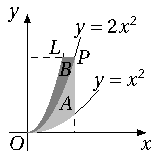
\includegraphics[scale=1]{figure/fig1-3-1.pdf}
			\caption{}\label{fig:1.3.1}
		\end{figure}
	\end{ti}

	\begin{ti}
		如图~\ref{fig:1.3.2} 所示,阴影部分由曲线 $y = \sin x(0 \leq x \leq \uppi)$,直线 $y = a(0 < a < 1)$,$x = \uppi$ 以及 $y$ 轴围成. 此图形绕直线 $y = a$ 旋转一周形成旋转体 $S$. 问 $a$ 为何值时,$S$ 有最小体积,$S$ 有最大体积.
		\begin{figure}[htbp]
			\centering
			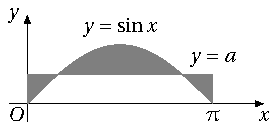
\includegraphics[scale=1]{figure/fig1-3-2.pdf}
			\caption{}\label{fig:1.3.2}
		\end{figure}
	\end{ti}

	\begin{ti}
		求曲线 $y^{2} = \bigl( 1 - x^{2} \bigr)^{3}$ 所围图形的面积.
	\end{ti}

	\begin{ti}
		求曲线 $\sqrt{x} + \sqrt{y} = 1$ 与坐标轴所围图形的面积.
	\end{ti}

	\begin{ti}
		求摆线 $x = t - \sin t$,$y = 1 - \cos t$ 的一拱与 $x$ 轴围成的图形的面积.
	\end{ti}

	\begin{ti}
		求星形线 $x = \cos^{3}t$,$y = \sin^{3}t$ 所围图形的面积.
	\end{ti}

	\begin{ti}
		求阿基米德螺线 $r = a \theta$ 的第一圈与极轴所围图形的面积.
	\end{ti}

	\begin{ti}
		求 $r = \sqrt{2} \sin \theta$ 及 $r^{2} = \cos 2 \theta$ 围成图形公共部分的面积.
	\end{ti}

	\begin{ti}
		求曲线 $y = \frac{1}{x^{2} + 1}$ 和 $x$ 轴之间区域的面积.
	\end{ti}

	\begin{ti}
		求曲线 $y = x \ee^{-\frac{x^{2}}{2}}$ 与其渐近线之间的面积.
	\end{ti}

	\begin{ti}
		记 $l_{1}$ 为椭圆 $x^{2} + 2y^{2} = 2$ 的周长,$l_{2}$ 为曲线 $y_{1} = \sin x$ 在 $0 \leq x \leq 2\uppi$ 上的弧长,$l_{3}$ 为曲线 $y_{2} = \frac{1}{2} \sin 2x$ 在 $0 \leq x \leq 2\uppi$ 上的弧长,则\kuo.

		\twoch{$l_{1} > l_{2} = l_{3}$}{$l_{1} = l_{2} < l_{3}$}{$l_{2} > l_{3} = l_{1}$}{$l_{1} = l_{2} = l_{3}$}
	\end{ti}

	\begin{ti}
		曲线 $\begin{cases}
			x = 3 (t - \sin t)\\
			y = 3 (1 - \cos t)
		\end{cases} (0 \leq t \leq 2\uppi)$ 的弧长为\htwo.
	\end{ti}

	\begin{ti}
		求抛物线 $6y = x^{2}$ 从点 $(0,0)$ 到点 $\bigl( 4,\frac{8}{3} \bigr)$ 之间的弧长.
	\end{ti}

	\begin{ti}
		求星形线 $x = \cos^{3}t$,$y = \sin^{3}t$ 的全长.
	\end{ti}

	\begin{ti}
		在摆线 $x = t - \sin t$,$y = 1 - \cos t$ 上求一点,将摆线第一拱的弧长分为 \ratio{$1$}{$3$}.
	\end{ti}

	\begin{ti}
		求心形线 $r = a (1 + \cos \theta)$ 的全长.
	\end{ti}

	\begin{ti}
		求曲线 $r \theta = 1$ 自 $\theta = \frac{3}{4}$ 至 $\theta = \frac{4}{3}$ 一段的弧长.
	\end{ti}

	\begin{ti}
		求曲线 $y = \int_{0}^{x} \sqrt{\cos t} \dd{t}$ 的全长.
	\end{ti}

	\begin{ti}
		当 $x \geq 0$ 时,曲线 $y = \frac{1}{4} \int_{0}^{2} x \sqrt{12 - x^{2} t^{2}} \dd{t}$ 的全长为\htwo.
	\end{ti}

	\begin{ti}
		设函数 $y = f(x)$ 在区间 $[0,1]$ 上非负、存在二阶导数,且 $f(0) = 0$,有一块质量均匀的平板 $D$,其占据的区域是曲线 $y = f(x)$ 与直线 $x = 1$ 以及 $x$ 轴围成的平面图形(图~\ref{fig:1.3.3}). 用 $\overline{x}$ 表示平板 $D$ 的质心的横坐标. 求证:
		\begin{enumerate}
			\item 若 $f'(x) > 0(0 \leq x \leq 1)$,则 $\overline{x} > \frac{1}{2}$(如图~\ref{fig:1.3.3:a});
			\item 若 $f''(x) > 0(0 \leq x \leq 1)$,则 $\overline{x} > \frac{2}{3}$(如图~\ref{fig:1.3.3:b}).
		\end{enumerate}
		\begin{figure}[htbp]
			\begin{floatrow}
			  \ffigbox[\textwidth]{
				\begin{subfloatrow}[2]
				  \ffigbox[\FBwidth]{
					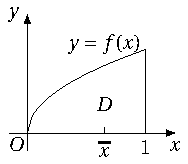
\includegraphics[scale=1]{figure/fig1-3-3-a.pdf}
				  }{\caption{}\label{fig:1.3.3:a}}
				  \ffigbox[\FBwidth]{
					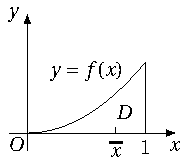
\includegraphics[scale=1]{figure/fig1-3-3-b.pdf}
				  }{\caption{}\label{fig:1.3.3:b}}
				\end{subfloatrow}
			  }{\caption{}\label{fig:1.3.3}}
			\end{floatrow}
		  \end{figure}
	\end{ti}

	\begin{ti}
		求由曲线 $y^{2} = x^{3} - x^{4}$ 所围成的平面图形的形心.
	\end{ti}

	\begin{ti}
		求由曲线 $y = x^{2}$ 与直线 $y = x$ 在第一象限内所围成的图形绕该直线旋转所成立体的体积.
	\end{ti}
	\subsection{一元积分的物理应用}

	\begin{ti}
		水从一根底面半径为 \SI{1}{cm} 的圆柱形管道中流出.因为水有黏性,在流动过程中受到管道壁的阻滞,所以流动的速度是随着到管道中心的距离而变化的. 距管道中心越远,水流速度越小. 在距离管道中心 $r$ \si{cm} 处的水的流动速度为 $10 \bigl(1 - r^{2}\bigr)$ \si{cm/s}. 问水是以多大流量(以 \si{cm^{3}/s} 为单位)流过管道的?
	\end{ti}

	\begin{ti}
		某城市的人口密度近似为 $p(r) = \frac{4}{r^{2} + 20}$,$p(r)$ 表示距市中心 $r$ \si{km} 区域的人口数,单位为每平方千米 $10$ 万人.
		\begin{enumerate}
			\item 试求距市中心 \SI{2}{km} 区域内的人口数;
			\item 若人口密度近似为 $p(r) = 1.2 \ee^{-0.2r}$ 单位不变,试求距市中心 \SI{2}{km} 区域内的人口数.
		\end{enumerate}
	\end{ti}

	\begin{ti}
		半径为 $1$ 的球沉入水中,球的上顶与水平面齐平. 球与水的密度相同记为 $\rho$,重力加速度记为 $g$,现将球打捞出水,至少需做多少功?
	\end{ti}

	\begin{ti}
		一个均质的物体,高 \SI{4}{m},水平截面面积是高度 $h$ (从底部算起)的函数 $S = 20 + 3h^{2}$. 已知物体的密度与水的密度同为 \SI{e3}{kg/m^3},此物体沉在水中,上表面与水面平齐,问将此物体打捞出水,至少需做功多少(设重力加速度 $g = $ \SI{10}{m/s^2})?
	\end{ti}

	\begin{ti}
		一块 \SI{1000}{kg} 的冰块要被吊起 \SI{30}{m} 高,而这块冰以 \SI{0.02}{kg/s} 的速度溶化,假设冰块以 \SI{0.1}{m/s} 的速度被吊起,吊索的线密度为 \SI{4}{kg/m}. 求把这块冰吊到指定高度需作的功(设重力加速度 $g = $ \SI{10}{m/s^2}).
	\end{ti}

	\begin{ti}
		\begin{enumerate}
			\item 宽度为 \SI{6}{m} 的金属板,三分之一作为侧边,做成排水沟(如图~\ref{fig:1.3.4}). 问折起角度多大时,排水沟的截面积 $S$ 最大;\label{3.142:1}
			\begin{figure}[htbp]
				\centering
				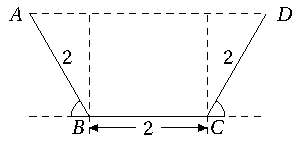
\includegraphics[scale=1]{figure/fig1-3-4.pdf}
				\caption{}\label{fig:1.3.4}
			\end{figure}
			\item 设一抛物线过(\ref{3.142:1})中所求得截面的 $A,D$ 及 $BC$ 中点,记该抛物线与直线段 $AD$ 所围成封闭平面的面积 $\widetilde{S}$,求 $\frac{S}{\widetilde{S}}$;\label{3.142:2}
			\item 若排水沟长为 \SI{1}{m},其横截面原为(\ref{3.142:1})中等腰梯形的形状,因淤泥沉积形成了(\ref{3.142:2})中抛物线的形状. 现清除淤泥,恢复(\ref{3.142:1})中的形状,将淤泥搬运出排水沟,则至少作多少功?(设单位体积的淤泥重为 $\rho$ \si{N/m^3})
		\end{enumerate}
	\end{ti}
	\subsection{平均值}

	\begin{ti}
		$f(x) = \int_{x}^{1} \cos t^{2} \dd{t}$ 在区间 $[0,1]$ 上的平均值为\htwo.
	\end{ti}

	\begin{ti}
		某质点以速度 $v = 3t^{2} + 2t$(\si{m/s})做直线运动,则它在 $t = 0$ 到 $t = $\SI{3}{s} 这段时间上的平均速度为\htwo.
	\end{ti}
	\subsection{一元积分不等式}

	\begin{ti}
		已知函数 $f(x)$ 在区间 $[a,b]$ 上连续并单调增加,求证:
		\[
			\int_{a}^{b} \Biggl( \frac{b - x}{b - a} \Biggr)^{n} f(x) \dd{x} \leq \frac{1}{n + 1} \int_{a}^{b} f(x) \dd{x} (n \in \mathbb N).
		\]
	\end{ti}

	\begin{ti}
		设 $f(x)$ 在 $[a,b]$ 上连续,且 $f(x) > 0$,证明:
		\[
			\ln \left[ \frac{1}{b - a} \int_{a}^{b} f(x) \dd{x} \right] \geq \frac{1}{b - a} \int_{a}^{b} \ln f(x) \dd{x}.
		\]
	\end{ti}

	\begin{ti}
		设 $f(x)$ 二阶可导,$f''(x) \geq 0$,$g(x)$ 为连续函数,若 $a > 0$,求证:
		\[
			\frac{1}{a} \int_{0}^{a} f\bigl[g(x)\bigr] \dd{x} \geq f\left[ \frac{1}{a} \int_{0}^{a} g(x) \dd{x} \right].
		\]
	\end{ti}

	\begin{ti}
		设 $f(x)$ 在闭区间 $[0,1]$ 上有二阶导数,且 $f\bigl( \frac{1}{2} \bigr) = 1$,$f''(x) > 0$,证明 $\int_{0}^{1} f(x) \dd{x} \geq 1$.
	\end{ti}

	\begin{ti}
		\begin{enumerate}
			\item 证明不等式
			\[
				\ln(n+1) < 1 + \frac{1}{2} + \frac{1}{3} + \cdots + \frac{1}{n} < 1 + \ln n;
			\]
			\item 证明数列 $a_{n} = 1 + \frac{1}{2} + \frac{1}{3} + \cdots + \frac{1}{n} - \ln(n+1)$ 单调增加,且 $0 < a_{n} < 1$.
		\end{enumerate}
	\end{ti}

	\begin{ti}
		当 $x \geq 0$ 时,在曲线 $y = \ee^{-2x}$ 上面作一个台阶曲线,台阶的宽度皆为 $1$(如图~\ref{fig:1.3.5}). 求图中无穷多个阴影部分的面积之和 $S$.
		\begin{figure}[htbp]
			\centering
			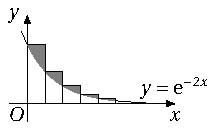
\includegraphics[scale=1]{figure/fig1-3-5.pdf}
			\caption{}\label{fig:1.3.5}
		\end{figure}
	\end{ti}

	\begin{ti}
		求极限 $\lim_{n \to \infty} \frac{\sum_{k=1}^{n} \frac{1}{k}}{\ln n}$.
	\end{ti}
	\section{多元函数微分学}
	\subsection{概念}

	\begin{ti}
		设 $f(x,y) = \ee^{x + y} \Bigl[ x^{\frac{1}{3}} (y - 1)^{\frac{1}{3}} + y^{\frac{1}{3}} (x - 1)^{\frac{2}{3}} \Bigr]$,则在点 $(0,1)$ 处的两个偏导数 $f_{x}'(0,1)$ 和 $f_{y}'(0,1)$ 的情况为\kuo.

		\onech{两个偏导数均不存在}{$f_{x}'(0,1)$ 不存在,$f_{y}'(0,1) = \frac{4}{3}\ee$}{$f_{x}'(0,1) = \frac{\ee}{3}$,$f_{y}'(0,1) = \frac{4}{3}\ee$}{$f_{x}'(0,1) = \frac{\ee}{3}$,$f_{y}'(0,1)$ 不存在}
	\end{ti}

	\begin{ti}
		函数 $z = f(x,y) = \sqrt{|xy|}$ 在点 $(0,0)$ \kuo.

		\onech{连续,但偏导数不存在}{偏导数存在,但不可微}{可微}{偏导数存在且连续}
	\end{ti}

	\begin{ti}
		函数 $f(x,y) = \sqrt[3]{x^{2} y}$ 在点 $(0,0)$ 处:
		\begin{enumerate}
			\item 是否连续,说明理由;
			\item 偏导数是否存在,说明理由;
			\item 是否可微,说明理由.
		\end{enumerate}
	\end{ti}

	\begin{ti}
		设
		\begin{enumerate}
			\item $f(x,y) = \begin{cases}
				\frac{x^{2} y^{2}}{\left( x^{2} + y^{2} \right)^{3/2}}, & (x,y) \ne (0,0),\\
				0, & (x,y) = (0,0);
			\end{cases}$
			\item $g(x,y) = \begin{cases}
				\bigl( x^{2} + y^{2} \bigr) \sin \frac{1}{x^{2} + y^{2}}, & (x,y) \ne (0,0),\\
				0, & (x,y) = (0,0).
			\end{cases}$
		\end{enumerate}
		讨论它们在点 $(0,0)$ 处的
		\begin{enumerate}
			\item[\libcirc{1}] 偏导数的存在性;
			\item[\libcirc{2}] 函数的连续性;
			\item[\libcirc{3}] 方向导数的存在性;
			\item[\libcirc{4}] 函数的可微性.
		\end{enumerate}
	\end{ti}

	\begin{ti}
		已知 $f(x,y) = \bigl( xy + xy^{2} \bigr) \ee^{x + y}$,则 $\frac{\partial^{10}f}{\partial x^{5} \partial y^{5}} = $\htwo.
	\end{ti}

	\begin{ti}
		\begin{enumerate}
			\item 设 $y = \frac{1}{x(1 - x)}$,求 $\frac{\dd^{n}y}{\dd{x^{n}}}$;
			\item 设 $z = \frac{y^{2}}{x(1 - x)}$,求 $\frac{\partial^{n}z}{\partial x^{n}}$.
		\end{enumerate}
	\end{ti}

	\begin{ti}
		设 $z = y^{2} \ln \bigl( 1 - x^{2} \bigr)$,求 $\frac{\partial^{n}z}{\partial x^{n}}$.
	\end{ti}

	\begin{ti}
		设 $z = x \ln \bigl[ \bigl( 1 + y^{2} \bigr) \ee^{x^{2} \sin y} \bigr]$,则 $\frac{\partial^{4}z}{\partial y^{2} \partial x^{2}} = $\htwo.
	\end{ti}

	\begin{ti}
		设函数 $f(x,y)$ 的一阶偏导数连续,在点 $(1,0)$ 的某邻域内有
		\[
			f(x,y) = 1 - x - 2y + o\left( \sqrt{(x - 1)^{2} + y^{2}} \right)
		\]
		成立. 记 $z(x,y) = f\bigl( \ee^{y}, x + y \bigr)$,则 $\dd{[z(x,y)]}|_{(0,0)} = $\htwo.
	\end{ti}

	\begin{ti}
		设函数 $f(x,y)$ 及它的二阶偏导数在全平面连续,且 $f(0,0) = 0$,$\Bigl| \frac{\partial f}{\partial x} \Bigr| \leq 2 \bigl|x - y\bigr|$,$\Bigl| \frac{\partial f}{\partial y} \Bigr| \leq 2 \bigl|x - y\bigr|$. 求证:$\bigl|f(5,4)\bigr| \leq 1$.
	\end{ti}

	\begin{ti}
		二元函数 $f(x,y) = x^{y}$ 在点 $(\ee,0)$ 处的二阶(即 $n = 2$) 泰勒展开式(不要求写出余项)为\htwo.
	\end{ti}
	\subsection{多元微分法}

	\begin{ti}
		设 $F(u,v)$ 对其变元 $u,v$ 具有二阶连续偏导数,并设 $z = F\bigl( \frac{y}{x},x^{2} + y^{2} \bigr)$,则 $\frac{\partial^{2}z}{\partial x \partial y} = $\htwo.
	\end{ti}

	\begin{ti}
		设 $u = y f \bigl( \frac{x}{y} \bigr) + x g \bigl( \frac{y}{x} \bigr)$,其中函数 $f,g$ 具有二阶连续偏导数,求 $x \frac{\partial^{2}u}{\partial x^{2}} + y \frac{\partial^{2}u}{\partial x \partial y}$.
	\end{ti}

	\begin{ti}
		设函数 $z = f(u)$,方程 $u = \varphi(u) + \int_{y}^{x} P(t) \dd{t}$ 确定 $u$ 是 $x,y$ 的函数,其中 $f(u),\varphi(u)$ 可微,$P(t),\varphi'(u)$ 连续,且 $\varphi'(u) \ne 1$. 求 $P(y) \frac{\partial z}{\partial x} + P(x) \frac{\partial z}{\partial y}$.
	\end{ti}

	\begin{ti}
		设 $f(x,y) = \int_{0}^{xy} \ee^{-t^{2}} \dd{t}$,求 $\frac{x}{y} \cdot \frac{\partial^{2}f}{\partial x^{2}} - 2 \frac{\partial^{2}f}{\partial x \partial y} + \frac{y}{x} \cdot \frac{\partial^{2}f}{\partial y^{2}}$.
	\end{ti}

	\begin{ti}
		设函数 $f(x,y)$ 可微,又 $f(0,0) = 0$,$f_{x}'(0,0) = a$,$f_{y}'(0,0) = b$,且 $\varphi(t) = f \bigl[ t, f \bigl( t, t^{2} \bigr) \bigr]$,求 $\varphi'(0)$.
	\end{ti}

	\begin{ti}
		设函数 $u = u(x,y)$ 满足 $\frac{\partial^{2}u}{\partial x^{2}} = \frac{\partial^{2}u}{\partial y^{2}}$ 及
		\[
			u(x,2x) = x,u_{1}'(x,2x) = x^{2},
		\]
		$u$ 有二阶连续偏导数,则 $u_{11}''(x,2x) = $\kuo.

		\fourch{$\frac{4}{3}x$}{$-\frac{4}{3}x$}{$\frac{3}{4}x$}{$-\frac{3}{4}x$}
	\end{ti}

	\begin{ti}
		若函数 $u = x y f \bigl( \frac{x + y}{xy} \bigr)$,其中 $f$ 是可微函数,且 $x^{2} \frac{\partial u}{\partial x} - y^{2} \frac{\partial u}{\partial y} = G(x,y) u$,则函数 $G(x,y) = $\kuo.

		\fourch{$x + y$}{$x - y$}{$x^{2} - y^{2}$}{$(x + y)^{2}$}
	\end{ti}

	\begin{ti}
		设函数 $u = f \bigl( \ln \sqrt{x^{2} + y^{2}} \bigr)$,满足 $\frac{\partial^{2}u}{\partial x^{2}} + \frac{\partial^{2}u}{\partial y^{2}} = \bigl( x^{2} + y^{2} \bigr)^{\frac{3}{2}}$,且极限
		\[
			\lim_{x \to 0} \frac{\int_{0}^{1} f(xt) \dd{t}}{x} = -1,
		\]
		试求函数 $f(x)$ 的表达式.
	\end{ti}

	\begin{ti}
		设 $u(x,y)$ 连续,证明无零值的函数 $u(x,y)$ 可分离变量(即 $u(x,y) = f(x) \cdot g(y)$)的充分必要条件是
		\[
			u \frac{\partial^{2}u}{\partial x \partial y} = \frac{\partial u}{\partial x} \frac{\partial u}{\partial y}.
		\]
	\end{ti}

	\begin{ti}
		设 $u = f(x,y,z)$ 有连续偏导数,$y = y(x)$ 和 $z = z(x)$ 分别由方程 $\ee^{xy} - y = 0$ 和 $\ee^{z} - xz = 0$ 所确定,求 $\frac{\dd{u}}{\dd{x}}$.
	\end{ti}

	\begin{ti}
		已知函数 $F(u,v,w)$ 可微,
		\[
			F_{u}'(0,0,0) = 1,
			F_{v}'(0,0,0) = 2,
			F_{w}'(0,0,0) = 3,
		\]
		函数 $z = f(x,y)$ 由 $F \bigl( 2x - y + 3z, 4x^{2} - y^{2} + z^{2}, xyz \bigr) = 0$ 确定,且满足 $f(1,2) = 0$,则 $f_{x}'(1,2) = $\htwo.
	\end{ti}

	\begin{ti}
		设 $u = f(x,y,z)$,$\varphi\bigl( x^{2},\ee^{y},z \bigr) = 0$,$y = \sin x$,其中 $f,\varphi$ 具有一阶连续的偏导数,且 $\frac{\partial \varphi}{\partial z} \ne 0$,求 $\frac{\dd{u}}{\dd{x}}$.
	\end{ti}

	\begin{ti}
		已知 $\begin{cases}
			z = x^{2} + y^{2},\\
			x^{2} + 2y^{2} + 3z^{2} = 20,
		\end{cases}$ 求 $\frac{\dd{y}}{\dd{x}},\frac{\dd{z}}{\dd{x}}$.
	\end{ti}

	\begin{ti}
		利用变量代换 $u = x$,$v = \frac{y}{x}$,可将方程
		\[
			x \frac{\partial z}{\partial x} + y \frac{\partial z}{\partial y} = z
		\]
		化成新方程\kuo.

		\twoch{$u \frac{\partial z}{\partial u} = z$}{$v \frac{\partial z}{\partial v} = z$}{$u \frac{\partial z}{\partial v} = z$}{$v \frac{\partial z}{\partial u} = z$}
	\end{ti}

	\begin{ti}
		已知函数 $u = u(x,y)$ 满足方程 $\frac{\partial^{2}u}{\partial x^{2}} - \frac{\partial^{2}u}{\partial y^{2}} + k \bigl( \frac{\partial u}{\partial x} + \frac{\partial u}{\partial y} \bigr) = 0$. 试确定参数 $a,b$,利用变换 $u(x,y) = v(x,y) \ee^{ax + by}$ 将原方程变形,使新方程中不含有一阶偏导数项.
	\end{ti}

	\begin{ti}
		设 $A,B,C$ 为常数,$B^{2} - AC > 0$,$A \ne 0$,$u(x,y)$ 具有二阶连续偏导数. 证明:必存在非奇异线性变换
		\[
			\xi = \lambda_{1}x + y, \eta = \lambda_{2}x + y(\lambda_{1},\lambda_{2} \text{ 为常数}),
		\]
		将方程 $A \frac{\partial^{2}u}{\partial x^{2}} + 2B \frac{\partial^{2}u}{\partial x \partial y} + C \frac{\partial^{2}u}{\partial y^{2}} = 0$ 化成 $\frac{\partial^{2}u}{\partial \xi \partial \eta} = 0$.
	\end{ti}

	\begin{ti}
		设 $h(t)$ 为三阶可导函数,$u = h(xyz)$,$h(1) = f_{xy}''(0,0)$,$h'(1) = f_{yx}''(0,0)$,且满足
		\[
			\frac{\partial^{3}u}{\partial x \partial y \partial z} = x^{2} y^{2} z^{2} h'''(xyz),
		\]
		求 $u$ 的表达式,其中
		\[
			f(x,y) = \begin{cases}
				x y \frac{x^{2} - y^{2}}{x^{2} + y^{2}}, & (x,y) \ne (0,0)\\
				0, & (x,y) = (0,0).
			\end{cases}
		\]
	\end{ti}

	\begin{ti}
		设 $z = z(u,v)$ 具有二阶连续偏导数,且 $z = z(x + y, x - y)$ 满足微分方程
		\[
			\frac{\partial^{2}z}{\partial x^{2}} + 2 \frac{\partial^{2}z}{\partial x \partial y} + \frac{\partial^{2}z}{\partial y^{2}} = 1.
		\]
		\begin{enumerate}
			\item 求 $z = z(u,v)$ 所满足关于 $u,v$ 的微分方程;\label{4.29:1}
			\item 由(\ref{4.29:1})求出 $z = z(x + y, x - y)$ 的一般表达式.
		\end{enumerate}
	\end{ti}

	\begin{ti}
		设 $f(u,v)$ 可微,证明曲面 $f(ax - bz, ay - cz) = 0$ 上任一点的切平面都与某一定直线平行,其中 $a,b,c$ 是不同时为零的常数.
	\end{ti}

	\begin{ti}
		证明曲面 $\ee^{2x - z} = f \bigl( \uppi y - \sqrt{2}z \bigr)$ 是柱面,其中 $f$ 可微.
	\end{ti}
	\subsection{多元函数的极值、最值问题}

	\begin{ti}
		函数
		\[
			f(x,y) = \begin{cases}
				\frac{\sin ( x^{2} + y^{2} )}{x^{2} + y^{2}}, & (x,y) \ne (0,0),\\
				1, & (x,y) = (0,0)
			\end{cases}
		\]
		在 $D = \bigl\{ (x,y) \bigl| x^{2} + y^{2} \leq 1 \bigr\}$ 上\kuo.

		\onech{有最大值,无最小值}{有最小值,无最大值}{既无最大值,又无最小值}{既有最大值,又有最小值}
	\end{ti}

	\begin{ti}
		设 $f(x,y)$ 在点 $(0,0)$ 的邻域内连续,且
		\[
			\lim_{(x,y) \to (0,0)} \frac{f(x,y) - 4xy}{x^{2} + y^{2}} = 1,
		\]
		则\kuo.

		\onech{点 $(0,0)$ 是 $f(x,y)$ 的极小值点}{点 $(0,0)$ 是 $f(x,y)$ 的极大值点}{点 $(0,0)$ 不是 $f(x,y)$ 的极值点}{所给条件不足以判断点 $(0,0)$ 是否为 $f(x,y)$ 的极值点}
	\end{ti}

	\begin{ti}
		设 $f(x,y)$ 是连续函数,且 $\lim_{\substack{x \to 0\\ y \to 0}} \frac{f(x,y) - f(0,0)}{x^{3} + y^{3} - 3x^{2} - 3y^{2}} = 1$,则\kuo.

		\onech{$f(0,0)$ 为 $f(x,y)$ 的极大值}{$f(0,0)$ 为 $f(x,y)$ 的极小值}{$f(0,0)$ 不是 $f(x,y)$ 的极值}{不能确定}
	\end{ti}

	\begin{ti}
		已知函数 $f(x,y)$ 在点 $(0,0)$ 的某邻域内连续,且
		\[
			\lim_{\substack{x \to 0\\ y \to 0}} \frac{f(x,y) - axy}{\bigl( x^{2} + y^{2} \bigr)^{2}} = 1,
		\]
		其中 $a$ 为非零常数,则 $f(0,0)$\kuo.

		\twoch{是极大值}{是极小值}{不是极值}{是否取极值与 $a$ 有关}
	\end{ti}

	\begin{ti}
		设 $f(x,y)$ 在点 $O(0,0)$ 的某邻域 $U$ 内连续,且 $\lim_{(x,y) \to (0,0)} \frac{f(x,y) - xy}{x^{2} + y^{2}} = a$,常数 $a > \frac{1}{2}$. 试讨论 $f(0,0)$ 是否为 $f(x,y)$ 的极值?若是极值,判断是极大值还是极小值?
	\end{ti}

	\begin{ti}
		设 $u(x,y)$ 在平面有界闭区域 $D$ 上具有二阶连续偏导数,且
		\[
			\frac{\partial^{2}u}{\partial x \partial y} \ne 0,\frac{\partial^{2}u}{\partial x^{2}} \cdot \frac{\partial^{2}u}{\partial y^{2}} = 0,
		\]
		则 $u(x,y)$ 的\kuo.

		\onech{最大值点和最小值点必定都在 $D$ 的内部}{最大值点和最小值点必定都在 $D$ 的边界上}{最大值点在 $D$ 的内部,最小值点在 $D$ 的边界上}{最小值点在 $D$ 的内部,最大值点在 $D$ 的边界上}
	\end{ti}

	\begin{ti}
		已知函数 $z = z(x,y)$ 在区域 $D$ 内满足方程 $\frac{\partial^{2}z}{\partial x^{2}} \cdot \frac{\partial^{2}z}{\partial y^{2}} + a \frac{\partial z}{\partial x} + b \frac{\partial z}{\partial y} + c = 0$(常数 $c > 0$),则在 $D$ 内函数 $z = z(x,y)$\kuo.

		\twoch{存在极大值}{存在极小值}{无极值}{无法判断}
	\end{ti}

	\begin{ti}
		函数 $z = x^{3} + y^{3} - 3x^{2} - 3y^{2}$ 的极小值点是\kuo.

		\fourch{$(0,0)$}{$(2,2)$}{$(0,2)$}{$(2,0)$}
	\end{ti}

	\begin{ti}
		若函数 $z = 2x^{2} + 2y^{2} + 3xy + ax + by + c$ 在点 $(-2,3)$ 处取得极小值 $-3$,则 $abc = $\htwo.
	\end{ti}

	\begin{ti}
		设函数 $z = z(x,y)$ 是由方程
		\[
			x^{2} - 6xy + 10y^{2} - 2yz - z^{2} + 32 = 0
		\]
		确定,讨论函数 $z(x,y)$ 的极大值与极小值.
	\end{ti}

	\begin{ti}
		函数 $f(x,y) = \ee^{-x} \bigl( ax + b - y^{2} \bigr)$,若 $f(-1,0)$ 为其极大值,则 $a,b$ 满足\htwo.
	\end{ti}

	\begin{ti}
		已知矩形的周长为 $2p$,将它绕其中一边旋转一周而构成一旋转体(圆柱体),求该圆柱体的半径与高各为多少时,该圆柱体体积最大?
	\end{ti}

	\begin{ti}
		\begin{enumerate}
			\item 设 $x > 0$,$y > 0$,$z > 0$,求函数 $f(x,y,z) = x y z^{3}$ 在约束条件 $x^{2} + y^{2} + z^{2} = 5 R^{2}$($R > 0$ 为常数)下的最大值;\label{4.44:1}
			\item 由(\ref{4.44:1})的结论证明:当 $a > 0$,$b > 0$,$c > 0$ 时,
			\[
				a b c^{3} \leq 27 \Biggl( \frac{a + b + c}{5} \Biggr)^{5}.
			\]
		\end{enumerate}
	\end{ti}

	\begin{ti}
		求二元函数 $z = f(x,y) = x^{2}y(4 - x - y)$ 在由直线 $x + y = 6$,$x$ 轴和 $y$ 轴所围成的闭区域 $D$ 上的极值、最大值与最小值.
	\end{ti}

	\begin{ti}
		求
		\[
			f(x,y) = x + xy - x^{2} - y^{2}
		\]
		在闭区域 $D = \{ (x,y) | 0 \leq x \leq 1, 0 \leq y \leq 2 \}$ 上的最大值和最小值.
	\end{ti}

	\begin{ti}
		求函数
		\[
			z = x^{2} + y^{2} + 2x + y
		\]
		在区域 $D = \bigl\{ (x,y) \bigl| x^{2} + y^{2} \leq 1 \bigr\}$ 上的最大值与最小值.
	\end{ti}

	\begin{ti}
		求内接于椭球面 $\frac{x^{2}}{a^{2}} + \frac{y^{2}}{b^{2}} + \frac{z^{2}}{c^{2}} = 1$ 的长方体的最大体积.
	\end{ti}

	\begin{ti}
		在第一象限的椭圆 $\frac{x^{2}}{4} + y^{2} = 1$ 上求一点,使过该点的法线与原点的距离最大.
	\end{ti}

	\begin{ti}
		设正数 $a,b$ 的值,使得椭圆 $\frac{x^{2}}{a^{2}} + \frac{y^{2}}{b^{2}} = 1$ 包含圆 $x^{2} + y^{2} = 2y$,且面积最小.
	\end{ti}

	\begin{ti}
		求证:$f(x,y) = Ax^{2} + 2Bxy + Cy^{2}$ 在约束条件 $1 - \frac{x^{2}}{a^{2}} - \frac{y^{2}}{b^{2}} = 0$ 下存在最大值和最小值,且它们是方程 $k^{2} - \bigl( Aa^{2} + Cb^{2} \bigr)k + \bigl( AC - B^{2} \bigr)a^{2}b^{2} = 0$ 的根.
	\end{ti}

	\begin{ti}
		曲面 $x^{2} + 2y^{2} + 3z^{2} = 1$ 的切平面与三个坐标平面围成的有限区域的体积的最小值为\htwo.
	\end{ti}

	\begin{ti}
		在 $xOz$ 面上有抛物线 $z = 2 - x^{2}$.
		\begin{enumerate}
			\item 求抛物线 $z = 2 - x^{2}$ 绕 $Oz$ 轴旋转所得的旋转抛物面方程;
			\item 在旋转抛物面位于第一卦限部分上求一点,使该点处的切平面与三坐标面围成的四面体的体积最小;
			\item 设 $V = \ln (4 - z)^{3} - 24 (\ln x + \ln y)$,其中 $x = x(y,z)$ 由方程 $z + x^{2} + y^{2} = 2$ 所确定,求 $\frac{\partial V}{\partial z}\bigl|_{(1,1,0)}$.
		\end{enumerate}
	\end{ti}

	\begin{ti}
		已知 $x,y,z$ 为实数,且 $\ee^{x} + y^{2} + |z| = 3$,求证 $\ee^{x} y^{2} |z| \leq 1$.
	\end{ti}
	\section{二重积分}
	\subsection{概念与性质}

	\begin{ti}
		计算 $\iint_{D} \bigl( x^{2} + y^{2} \bigr)^{\frac{3}{2}} \dd{\sigma}$,其中 $D = \bigl\{ (x,y) \bigl| x^{2} + y^{2} \leq 1, x^{2} + y^{2} \leq 2x \bigr\}$.
	\end{ti}

	\begin{ti}
		计算 $\iint_{D} \sqrt{x^{2} + y^{2}} \dd{x} \dd{y}$,其中 $D = \bigl\{ (x,y) \bigl| 0 \leq x \leq 1, 0 \leq y \leq 1 \bigr\}$.
	\end{ti}

	\begin{ti}
		计算
		\[
			I = \iint_{D} \frac{1 + y + y \ln \bigl( x + \sqrt{1 + x^{2}} \bigr)}{1 + x^{2} + y^{2}} \dd{\sigma},
		\]
		其中 $D = \bigl\{ (x,y) \bigl| x^{2} + y^{2} \leq 1, x \geq 0 \bigr\}$.
	\end{ti}

	\begin{ti}
		设 $f(x)$ 为连续的奇函数,平面区域 $D$ 由 $y = -x^{3}$,$x = 1$ 与 $y = 1$ 围成,计算 $I = \iint_{D} \bigl[ x^{2} + f(xy) \bigr] \dd{\sigma}$.
	\end{ti}

	\begin{ti}
		若 $D$ 是由直线 $x = -2$,$y = 0$,$y = 2$ 以及曲线 $x = -\sqrt{2y - y^{2}}$ 所围成的平面区域,计算 $I = \iint_{D} y \dd{x} \dd{y}$.
	\end{ti}

	\begin{ti}
		若 $D$ 是由圆 $x^{2} + y^{2} = 4$ 与 $(x + 1)^{2} + y^{2} = 1$ 所围成的平面区域(如图~\ref{fig:1.5.1}),计算 $I = \iint_{D} \bigl( \sqrt{x^{2} + y^{2}} + y \bigr) \dd{\sigma}$.
		\begin{figure}[htbp]
			\centering
			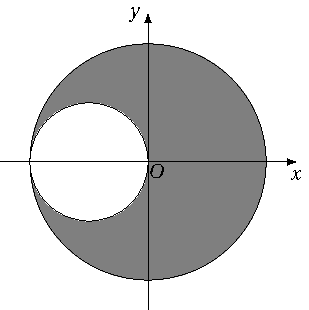
\includegraphics[scale=1]{figure/fig1-5-1.pdf}
			\caption{}\label{fig:1.5.1}
		\end{figure}
	\end{ti}

	\begin{ti}
		设 $D = \bigl\{ (x,y) \bigl| x^{2} + y^{2} \leq 1 \text{\ 且\ } x + y \geq 0 \bigr\}$,$f$ 为连续函数,计算
		\[
			I = \iint_{D} xy \bigl[ x + f\bigl( x^{2} - y^{2} \bigr) \bigr] \dd{x} \dd{y}.
		\]
	\end{ti}

	\begin{ti}
		设 $I(a) = \iint_{D} (x + y) \dd{x} \dd{y}$,其中 $D$ 由直线 $x = a$,$x = 0$,$y = a$,$y = -a$ 及曲线 $x^{2} + y^{2} = ax(a > 0)$ 所围成,计算 $I(a)$.
	\end{ti}

	\begin{ti}
		$\int_{-1}^{1} \dd{x} \int_{|x|}^{\sqrt{2 - x^{2}}} \sin \bigl( x^{2} + y^{2} \bigr) \dd{y} = $\kuo.

		\twoch{$\frac{\uppi}{4}(\cos 2 - 1)$}{$\frac{\uppi}{4}(- \cos 2 + 1)$}{$\frac{\uppi}{4}(\cos 2 + 1)$}{$\frac{\uppi}{4}(- \cos 2 - 1)$}
	\end{ti}

	\begin{ti}
		设平面区域 $D$ 由曲线 $y = \sin x \bigl( - \frac{\uppi}{2} \leq x \leq \frac{\uppi}{2} \bigr)$,$x = -\frac{\uppi}{2}$,$y = 1$ 围成,则 $\iint_{D} \bigl( xy^{3} - 1 \bigr) \dd{\sigma}$ 等于\kuo.

		\fourch{$2$}{$-2$}{$\uppi$}{$-\uppi$}
	\end{ti}

	\begin{ti}
		记平面区域 $D = \bigl\{ (x,y) \bigl| |x| + |y| \leq 1 \bigr\}$,计算如下二重积分:
		\begin{enumerate}
			\item $I_{1} = \iint_{D} \frac{af(x) + bf(y)}{f(x) + f(y)} \dd{\sigma}$,其中 $f(t)$ 为定义在 $(-\infty,$ $+\infty)$ 内的连续正值函数,常数 $a > 0, b > 0$;
			\item $I_{2} = \iint_{D} \bigl( \ee^{\lambda x} - \ee^{-\lambda y} \bigr) \dd{\sigma}$,常数 $\lambda > 0$.
		\end{enumerate}
	\end{ti}

	\begin{ti}
		设 $p(x)$ 在 $[a,b]$ 上非负且连续,$f(x)$ 与 $g(x)$ 在 $[a,b]$ 上连续且有相同的单调性,其中
		\[
			D = \bigl\{ (x,y) \bigl| a \leq x \leq b, a \leq y \leq b \bigr\},
		\]
		比较
		\begin{align*}
			I_{1} &= \iint_{D} p(x) f(x) p(y) g(y) \dd{x} \dd{y},\\
			I_{2} &= \iint_{D} p(x) f(y) p(y) g(y) \dd{x} \dd{y}
		\end{align*}
		的大小,并说明理由.
	\end{ti}
	\subsection{积分比大小}

	\begin{ti}
		设
		\begin{align*}
			a &= \iint_{D} \cos \sqrt{x^{2} + y^{2}} \dd{\sigma},\\
			b &= \iint_{D} \cos \bigl( x^{2} + y^{2} \bigr) \dd{\sigma},\\
			c &= \iint_{D} \cos \bigl( x^{2} + y^{2} \bigr)^{2} \dd{\sigma},
		\end{align*}
		其中 $D = \bigl\{ (x,y) \bigl| x^{2} + y^{2} \leq 1 \bigr\}$,则\kuo.

		\twoch{$c > b > a$}{$a > b > c$}{$b > a > c$}{$c > a > b$}
	\end{ti}

	\begin{ti}
		设平面区域 $D$ 由 $x = 0$,$y = 0$,$x + y = \frac{1}{4}$,$x + y = 1$ 围成,若 $I_{1} = \iint_{D} \bigl[ \ln (x+y) \bigr]^{3} \dd{x} \dd{y}$,$I = \iint_{D} (x + y)^{3} \dd{x} \dd{y}$,$I_{3} = \iint_{D} \bigl[ \sin(x + y) \bigr]^{3} \dd{x} \dd{y}$,则 $I_{1},I_{2},I_{3}$ 的大小顺序为\kuo.

		\twoch{$I_{1} < I_{2} < I_{3}$}{$I_{3} < I_{2} < I_{1}$}{$I_{1} < I_{3} < I_{2}$}{$I_{3} < I_{1} < I_{2}$}
	\end{ti}

	\begin{ti}
		设平面区域 $D = \bigl\{ (x,y) \bigl| (x - 2)^{2} + (y - 1)^{2} \leq 1 \bigr\}$,若比较 $I_{1} = \iint_{D} (x + y)^{2} \dd{\sigma}$ 与 $I_{2} = \iint_{D} (x + y)^{3} \dd{\sigma}$ 的大小,则有\kuo.

		\twoch{$I_{1} = I_{2}$}{$I_{1} > I_{2}$}{$I_{1} < I_{2}$}{不能比较}
	\end{ti}
	\subsection{计算}
	
	\begin{ti}
		计算 $I = \int_{1}^{2} \dd{x} \int_{\frac{1}{x}}^{1} y \ee^{xy} \dd{y}$.
	\end{ti}

	\begin{ti}
		\[
			\int_{0}^{1} \dd{y} \int_{0}^{1} \sqrt{\ee^{2x} - y^{2}} \dd{x} + \int_{1}^{\ee} \dd{y} \int_{\ln y}^{1} \sqrt{\ee^{2x} - y^{2}} \dd{x} = 
		\]
		\kuo.

		\twoch{$\frac{\uppi}{8}\bigl( \ee^{2} - 1 \bigr)$}{$\frac{\uppi}{8}\bigl( \ee^{2} + 1 \bigr)$}{$\frac{\uppi}{4}\bigl( \ee^{2} - 1 \bigr)$}{$\frac{\uppi}{4}\bigl( \ee^{2} + 1 \bigr)$}
	\end{ti}

	\begin{ti}
		已知
		\[
			I = \int_{0}^{2} \dd{x} \int_{0}^{\frac{x^{2}}{2}} f(x,y) \dd{y} + \int_{2}^{2\sqrt{2}} \dd{x} \int_{0}^{\sqrt{8 - x^{2}}} f(x,y) \dd{y},
		\]
		则 $I = $\kuo.

		\onech{$\int_{0}^{2} \dd{y} \int_{\sqrt{2y}}^{\sqrt{8 - y^{2}}} f(x,y) \dd{x}$}{$\int_{0}^{2} \dd{y} \int_{1}^{\sqrt{8 - y^{2}}} f(x,y) \dd{x}$}{$\int_{0}^{1} \dd{y} \int_{\sqrt{2y}}^{\sqrt{8 - y^{2}}} f(x,y) \dd{x}$}{$\int_{0}^{2} \dd{y} \int_{\sqrt{2y}}^{1} f(x,y) \dd{x}$}
	\end{ti}

	\begin{ti}
		累次积分 $\int_{0}^{2R} \dd{y} \int_{0}^{\sqrt{2Ry - y^{2}}} f \bigl( x^{2} + y^{2} \bigr) \dd{x} (R > 0)$ 化为极坐标形式的累次积分为\kuo.

		\onech{$\int_{0}^{\uppi} \dd{\theta} \int_{0}^{2R\sin\theta} f \bigl( r^{2} \bigr) r \dd{r}$}{$\int_{0}^{\frac{\uppi}{2}} \dd{\theta} \int_{0}^{2R\cos\theta} f \bigl( r^{2} \bigr) r \dd{r}$}{$\int_{0}^{\frac{\uppi}{2}} \dd{\theta} \int_{0}^{2R\sin\theta} f \bigl( r^{2} \bigr) r \dd{r}$}{$\int_{0}^{\uppi} \dd{\theta} \int_{0}^{2R\cos\theta} f \bigl( r^{2} \bigr) r \dd{r}$}
	\end{ti}

	\begin{ti}
		计算 $\int_{0}^{1} \dd{y} \int_{\arcsin y}^{\frac{\uppi}{2}} \cos x \cdot \sqrt{1 + \cos^{2}x} \dd{x}$.
	\end{ti}

	\begin{ti}
		计算 $\int_{0}^{1} \dd{y} \int_{3y}^{3} \ee^{x^{2}} \dd{x}$.
	\end{ti}

	\begin{ti}
		计算 $\int_{0}^{1} \dd{y} \int_{\sqrt{y}}^{1} \sqrt{x^{3} + 1} \dd{x}$.
	\end{ti}

	\begin{ti}
		计算 $\int_{0}^{1} \dd{x} \int_{x^{2}}^{1} x^{3} \sin y^{3} \dd{y}$.
	\end{ti}

	\begin{ti}
		计算 $\int_{0}^{1} \dd{x} \int_{x^{2}}^{x} \bigl( x^{2} + y^{2} \bigr)^{-\frac{1}{2}} \dd{y}$.
	\end{ti}

	\begin{ti}
		计算 $\int_{1}^{2} \dd{x} \int_{0}^{x} \frac{y \sqrt{x^{2} + y^{2}}}{x} \dd{y}$.
	\end{ti}

	\begin{ti}
		计算 $\int_{1}^{2} \dd{x} \int_{\sqrt{x}}^{x} \sin \frac{\uppi x}{2y} \dd{y} + \int_{2}^{4} \dd{x} \int_{\sqrt{x}}^{2} \sin \frac{\uppi x}{2y} \dd{y}$.
	\end{ti}

	\begin{ti}
		$\int_{0}^{1} \dd{y} \int_{y}^{1} \Bigl( \frac{\ee^{x^{2}}}{x} - \ee^{y^{2}} \Bigr) \dd{x} = $\htwo.
	\end{ti}

	\begin{ti}
		计算 $\iint_{D} \ee^{\frac{y}{x + y}} \dd{\sigma}$,其中 $D = \bigl\{ (x,y) \bigl| 0 \leq y \leq 1 - x, y \leq x \bigr\}$.
	\end{ti}

	\begin{ti}
		设平面区域 $D = \Bigl\{ (x,y) \Bigl| x^{2} + y^{2} \leq 8, y \geq \frac{x^{2}}{2} \Bigr\}$,计算
		\[
			I = \iint_{D} \bigl[ (x - 1)^{2} + y^{2} \bigr] \dd{\sigma}.
		\]
	\end{ti}

	\begin{ti}
		计算
		\[
			I = \iint_{D} \bigl( x^{2} + xy \bigr)^{2} \dd{x} \dd{y},
		\]
		其中 $D = \bigl\{ (x,y) \bigl| x^{2} + y^{2} \leq 2x \bigr\}$.
	\end{ti}

	\begin{ti}
		计算 $I = \iint_{\sqrt{x} + \sqrt{y} \leq 1} \sqrt[3]{\sqrt{x} + \sqrt{y}} \dd{x} \dd{y}$.
	\end{ti}

	\begin{ti}
		设函数 $f(x,y)$ 连续,且
		\[
			f(x,y) = x + \iint_{D} y f(u,v) \dd{u} \dd{v},
		\]
		其中 $D$ 由 $y = \frac{1}{x}$,$x = 1$,$y = 2$ 围成,求 $f(x,y)$.
	\end{ti}

	\begin{ti}
		设 $D = \bigl\{ (x,y) \bigl| |x| \leq 2, |y| \leq 2 \bigr\}$,计算
		\[
			I = \iint_{D} \bigl| x^{2} + y^{2} - 1 \bigr| \dd{\sigma}.
		\]
	\end{ti}

	\begin{ti}
		设 $D = \bigl\{ (x,y) \bigl| 0 \leq x \leq 1, 0 \leq y \leq 2\ee \bigr\}$,计算
		\[
			\iint_{D} x \bigl| y - \ee^{x} \bigr| \dd{\sigma}.
		\]
	\end{ti}

	\begin{ti}
		计算 $I = \iint_{D} \bigl( |x| + |y| \bigr) \dd{x} \dd{y}$,其中 $D$ 是由曲线 $xy = 2$,直线 $y = x - 1$ 及 $y = x + 1$ 所围成的区域.
	\end{ti}

	\begin{ti}
		设 $D = \bigl\{ (x,y) \bigl| 0 \leq x \leq \uppi, 0 \leq y \leq 2 \bigr\}$,计算 $\iint_{D} \bigl| y - \sin x \bigr| \dd{\sigma}$.
	\end{ti}

	\begin{ti}
		计算
		\[
			I = \int_{-1}^{1} \dd{x} \int_{x}^{2 - |x|} \bigl[ \ee^{|y|} + \sin \bigl( x^{3}y^{3} \bigr) \bigr] \dd{y}.
		\]
	\end{ti}

	\begin{ti}
		设 $f(x,y) = \begin{cases}
			1 - x - y, & x + y \leq 1,\\
			2, & x + y > 1,
		\end{cases}$ 计算
		\[
			\iint_{D} f(x,y) \dd{x} \dd{y},
		\]
		其中 $D$ 为正方形区域 $\bigl\{ (x,y) \bigl| 0 \leq x \leq 1, 0 \leq y \leq 1 \bigr\}$.
	\end{ti}

	\begin{ti}
		设函数 $f(x) = \begin{cases}
			x, & 0 \leq x \leq 2,\\
			0, & x < 0 \text{\ 或\ } x > 2,
		\end{cases}$ 计算 $I = \iint_{D} \frac{f(x + y)}{f\left( \sqrt{x^{2} + y^{2}} \right)} \dd{x} \dd{y}$,其中 $D = \bigl\{ (x,y) \bigl| x^{2} + y^{2} \leq 4 \bigr\}$.
	\end{ti}

	\begin{ti}
		计算 $\iint_{D} \min\bigl\{ x,y \bigr\} \dd{x} \dd{y}$,其中 $D = \bigl\{ (x,y) \bigl| 0 \leq x \leq 3, 0 \leq y \leq 1 \bigr\}$.
	\end{ti}

	\begin{ti}
		计算 $\int_{0}^{a} \dd{x} \int_{0}^{b} \ee^{ \max\left\{ b^{2}x^{2}, a^{2}y^{2} \right\} } \dd{y}$,其中 $a,b > 0$.
	\end{ti}

	\begin{ti}
		设 $F(x,y) = \frac{\partial^{2}f(x,y)}{\partial x \partial y}$ 在 $D = [a,b] \times [c,d]$ 上连续,求
		\[
			I = \iint_{D} F(x,y) \dd{x} \dd{y},
		\]
		并证明:$I \leq 2(M - m)$,其中 $M$ 和 $m$ 分别是 $f(x,y)$ 在 $D$ 上的最大值和最小值.
	\end{ti}

	\begin{ti}
		设函数 $f(x)$ 在 $[0,1]$ 上连续,证明:
		\[
			\int_{0}^{1} \ee^{f(x)} \dd{x} \int_{0}^{1} \ee^{-f(y)} \dd{y} \geq 1.
		\]
	\end{ti}

	\begin{ti}
		设 $f(x,y)$ 为连续函数,则
		\[
			I = \lim_{t \to 0^{+}} \frac{1}{\uppi t^{2}} \iint_{D} f(x,y) \dd{\sigma}
		\] = \htwo,其中 $D = \bigl\{ (x,y) \bigl| x^{2} + y^{2} \leq t^{2} \bigr\}$.
	\end{ti}

	\begin{ti}
		已知 $f(t) = \iint_{D(t): x^{2} + y^{2} \leq t^{2}} \bigl( \ee^{x^{2} + y^{2}} - ky^{2} \bigr) \dd{\sigma}$ 在 $t \in (0,+\infty)$ 内是单调增加函数,$k$为常数,求 $k$ 的最大取值范围.
	\end{ti}

	\begin{ti}
		由曲线 $y = x^{2}$,$y = x + 2$ 所围成的平面薄片,其上各点处的面密度 $\mu = 1 + x^{2}$,则此薄片的质量 $M = $\htwo.
	\end{ti}

	\begin{ti}
		求柱体 $x^{2} + y^{2} \leq 2x$ 被 $x^{2} + y^{2} + z^{2} = 4$ 所截得部分的体积.
	\end{ti}

	\begin{ti}
		设平面薄片所占的区域 $D$ 由抛物线 $y = x^{2}$ 及直线 $y = x$ 所围成,它在 $(x,y)$ 处的面密度 $\rho(x,y) = x^{2}y$,求此薄片的重心.
	\end{ti}
	\section{代数与几何}

	\begin{ti}
		已知曲面 $z = x^{2} + y^{2}$ 上点 $P$ 处的切平面平行于平面 $2x + 2y + z - 1 = 0$,则点 $P$ 的坐标是\kuo.

		\twoch{$(1,-1,2)$}{$(-1,1,2)$}{$(1,1,2)$}{$(-1,-1,2)$}
	\end{ti}

	\begin{ti}
		过点 $P(2,0,3)$ 且与直线 $\begin{cases}
			x - 2y + 4z - 7 = 0,\\
			3x + 5y - 2z + 1 = 0
		\end{cases}$ 垂直的平面的方程是\kuo.

		\onech{$(x-2) - 2(y-0) + 4(z-3) = 0$}{$3(x-2) + 5(y-0) - 2(z-3) = 0$}{$-16(x-2) + 14(y-0) + 11(z-3) = 0$}{$-16(x+2) + 14(y-0) + 11(z-3) = 0$}
	\end{ti}

	\begin{ti}
		已知 $|\bm a| = 1$,$|\bm b| = \sqrt{2}$,且 $( \widehat{ \bm a, \bm b } ) = \frac{\uppi}{4}$,则 $|\bm a + \bm b| = $\kuo.

		\fourch{$1$}{$1 + \sqrt{2}$}{$2$}{$\sqrt{5}$}
	\end{ti}

	\begin{ti}
		曲线 $x^{2} + y^{2} + z^{2} = a^{2}$ 与 $x^{2} + y^{2} = 2az(a > 0)$ 的交线是\kuo.

		\fourch{抛物线}{双曲线}{圆}{椭圆}
	\end{ti}

	\begin{ti}
		若非零向量 $\bm a, \bm b$ 满足关系式 $|\bm a - \bm b| = |\bm a + \bm b|$,则必有\kuo.

		\twoch{$\bm a - \bm b = \bm a + \bm b$}{$\bm a = \bm b$}{$\bm a \cdot \bm b = 0$}{$\bm a \times \bm b = \bm 0$}
	\end{ti}

	\begin{ti}
		若 $\bm a \perp \bm b$,$\bm a, \bm b$ 均为非零向量,$x$ 是非零实数,则有\kuo.

		\twoch{$|\bm a + x \bm b| > |\bm a| + |x| |\bm b|$}{$|\bm a - x \bm b| < |\bm a| - |x| |\bm b|$}{$|\bm a + x \bm b| > |\bm a|$}{$|\bm a - x \bm b| < |\bm a|$}
	\end{ti}

	\begin{ti}
		在曲线 $x = t, y = -t^{2}, z = t^{3}$ 的所有切线中,与平面 $x + 2y + z = 4$ 平行的切线\kuo.

		\twoch{只有 $1$ 条}{只有 $2$ 条}{至少有 $3$ 条}{不存在}
	\end{ti}

	\begin{ti}
		两条平行直线
		\begin{align*}
			L_{1}&: \begin{cases}
				x = 1 + t,\\
				y = -1 + 2t,\\
				z = t,
			\end{cases},\\
			L_{2}&: \begin{cases}
				x = 2 + t,\\
				y = -1 + 2t,\\
				z = 1 + t
			\end{cases},
		\end{align*}
		之间的距离为\kuo.

		\fourch{$\frac{2}{3}$}{$\frac{2}{3}\sqrt{3}$}{$1$}{$2$}
	\end{ti}

	\begin{ti}
		与直线 $L_{1}: \begin{cases}
			x = 1,\\
			y = -2 + t,\\
			z = 1 + t
		\end{cases}$ 及直线
		\[
			L_{2}: \frac{x + 1}{1} = \frac{y + 1}{2} = \frac{z - 1}{1}
		\]
		都平行,且过原点的平面 $\pi$ 的方程为\kuo.

		\twoch{$x + y + z = 0$}{$x - y + z = 0$}{$x + y - z = 0$}{$x - y + z + 2 = 0$}
	\end{ti}

	\begin{ti}
		直线 $L: \frac{x - 2}{2} = \frac{y - 1}{1} = \frac{z - 3}{1}$ 与平面 $\pi: x - y + 2z + 4 = 0$ 的夹角为\kuo.

		\fourch{$\pi$}{$\frac{\pi}{3}$}{$\frac{\pi}{6}$}{$\frac{\pi}{2}$}
	\end{ti}

	\begin{ti}
		已知等边三角形 $\triangle ABC$ 的边长为 $1$,且 $\overrightarrow{BC} = \bm a$,$\overrightarrow{CA} = \bm b$,$\overrightarrow{AB} = \bm c$,则 $\bm a \cdot \bm b + \bm b \cdot \bm c + \bm c \cdot \bm a = $\kuo.

		\fourch{$\frac{1}{2}$}{$\frac{2}{3}$}{$-\frac{1}{2}$}{$-\frac{3}{2}$}
	\end{ti}

	\begin{ti}
		设直线 $L$ 为 $\begin{cases}
			x + 3y + 2z + 1 = 0,\\
			2x - y - 10z + 3 = 0,
		\end{cases}$ 平面 $\pi$ 为 $4x - 2y + z - 2 = 0$,则\kuo.

		\twoch{$L$ 平行于 $\pi$}{$L$ 在 $\pi$ 上}{$L$ 垂直于 $\pi$}{$L$ 与 $\pi$ 相交但不垂直}
	\end{ti}

	\begin{ti}
		设 $\bm a$ 与 $\bm b$ 为非零向量,则 $\bm a \times \bm b = \bm 0$ 是\kuo.

		\onech{$\bm a = \bm b$ 的充要条件}{$\bm a \perp \bm b$ 的充要条件}{$\bm a \parallel \bm b$ 的充要条件}{$\bm a \parallel \bm b$ 的必要但不充分条件}
	\end{ti}

	\begin{ti}
		设 $\bm c = \alpha \bm a + \beta \bm b$,$\bm a, \bm b$ 为非零向量,且 $\bm a$ 与 $\bm b$ 不平行. 若这些向量起点相同,且 $\bm a, \bm b, \bm c$ 的终点在同一直线上,则必有\kuo.

		\twoch{$\alpha \beta \geq 0$}{$\alpha \beta \leq 0$}{$\alpha + \beta = 1$}{$\alpha^{2} + \beta^{2} = 1$}
	\end{ti}

	\begin{ti}
		设有直线
		\[
			L_{1}: \frac{x - 1}{1} = \frac{y - 5}{-2} = \frac{z + 8}{1}
		\]
		与 $L_{2}: \begin{cases}
			x - y = 6,\\
			2y + z = 3,
		\end{cases}$ 则 $L_{1}$ 与 $L_{2}$ 的夹角为\kuo.

		\fourch{$\frac{\pi}{3}$}{$\frac{\pi}{6}$}{$\frac{\pi}{4}$}{$\frac{\pi}{2}$}
	\end{ti}

	\begin{ti}
		曲线 $S: \begin{cases}
			x^{2} + y^{2} + z^{2} = 2,\\
			x + y + z = 0
		\end{cases}$ 在点 $(1,-1,0)$ 处的切线方程为\kuo.

		\twoch{$\frac{x - 1}{2} = \frac{y + 1}{1} = \frac{z}{1}$}{$\frac{x - 1}{2} = \frac{y + 1}{2} = \frac{z}{3}$}{$\frac{x - 1}{-1} = \frac{y + 1}{-1} = \frac{z}{1}$}{$\frac{x - 1}{1} = \frac{y + 1}{1} = \frac{z}{-2}$}
	\end{ti}

	\begin{ti}
		曲面 $x^{\frac{2}{3}} + y^{\frac{2}{3}} + z^{\frac{2}{3}} = 4$ 上任一点的切平面在三个坐标轴上的截距的平方和为\kuo.

		\fourch{$48$}{$64$}{$36$}{$16$}
	\end{ti}

	\begin{ti}
		以下 $4$ 个平面方程:\libcirc{1}$7x + 5y + 2z + 10 = 0$,\libcirc{2}$-7x - 5y + 2z - 10 = 0$,\libcirc{3}$7x - y + 14z + 26 = 0$,\libcirc{4}$x - 7y + 14z - 26 = 0$,是平面 $x + 2y - 2z + 6 = 0$ 和平面 $4x - y + 8z - 8 = 0$ 的交角的平分面方程的是\kuo.

		\fourch{\circled{1}\circled{2}}{\circled{2}\circled{3}}{\circled{2}\circled{4}}{\circled{1}\circled{4}}
	\end{ti}

	\begin{ti}
		已知 $|\bm a| = 2$,$|\bm b| = 2$,$(\widehat{\bm a, \bm b}) = \frac{\uppi}{3}$,则 $\bm u = 2 \bm a - 3 \bm b$ 的模 $|\bm u| = $\htwo.
	\end{ti}

	\begin{ti}
		设 $\bm A = 2 \bm a + \bm b$,$\bm B = k \bm a + \bm b$,其中 $|\bm a| = 1$,$|\bm b| = 2$,且 $\bm a \perp \bm b$. 若 $\bm A \perp \bm B$,则 $k = $\htwo.
	\end{ti}

	\begin{ti}
		点 $(-1,2,0)$ 在平面 $x + 2y - z + 1 = 0$ 上的投影为\htwo.
	\end{ti}

	\begin{ti}
		点 $(1,2,1)$ 到平面 $x + 2y + 2z - 13 = 0$ 的距离是
		
		\noindent\htwo.
	\end{ti}

	\begin{ti}
		过三点 $A(1,1,-1), B(-2,-2,2)$ 和 $C(1,-1,2)$ 的平面方程是\htwo.
	\end{ti}

	\begin{ti}
		$xOz$ 坐标面上的抛物线 $z^{2} = x - 2$ 绕 $x$ 轴旋转而成的旋转抛物面的方程是\htwo.
	\end{ti}

	\begin{ti}
		设 $\bm a, \bm b, \bm c$ 的模 $|\bm a| = |\bm b| = |\bm c| = 2$,且满足 $\bm a + \bm b + \bm c = \bm 0$,则 $\bm a \cdot \bm b + \bm b \cdot \bm c + \bm c \cdot \bm a = $\htwo.
	\end{ti}

	\begin{ti}
		经过点 $A(1,0,0)$ 与点 $B(0,1,1)$ 的直线绕 $z$ 轴旋转一周生成的曲面方程是\htwo.
	\end{ti}

	\begin{ti}
		已知直线
		\[
			L_{1}: \begin{cases}
				x + y = 0,\\
				2y + z + 1 = 0
			\end{cases}
		\]
		和
		\[
			L_{2}: \begin{cases}
				x = 1 - t,\\
				y = -1 + 2t,\\
				z = 1 + t,
			\end{cases}
		\]
		则过直线 $L_{1}$ 和 $L_{2}$ 的平面是\htwo.
	\end{ti}

	\begin{ti}
		过直线 $\begin{cases}
			x = 1 + t,\\
			y = 1 + 2t,\\
			z = 1 + 3t
		\end{cases}$ 且和点 $(2,2,2)$ 的距离为 $\frac{1}{\sqrt{3}}$ 的平面方程是\htwo.
	\end{ti}

	\begin{ti}
		曲面 $z - \ee^{z} + 2xy = 3$ 在点 $(1,2,0)$ 处的切平面方程为\htwo.
	\end{ti}

	\begin{ti}
		点 $(1,2,3)$ 到直线 $\frac{x}{1} = \frac{y - 4}{-3} = \frac{z - 3}{-2}$ 的距离为\htwo.
	\end{ti}

	\begin{ti}
		设 $\bm a = 3 \bm i + 4 \bm k$,$\bm b = - \bm i + 2 \bm j - 2 \bm k$,求与向量 $\bm a$ 和 $\bm b$ 均垂直的单位向量.
	\end{ti}

	\begin{ti}
		求到平面 $2x - 3y + 6z - 4 = 0$ 和平面 $12x - 15y + 16z - 1 = 0$ 距离相等的点的轨迹方程.
	\end{ti}

	\begin{ti}
		求过两点 $A(0,1,0), B(-1,2,1)$ 且与直线
		\[
			\begin{cases}
				x = -2 + t,\\
				y = 1 - 4t,\\
				z = 2 + 3t
			\end{cases}
		\]
		平行的平面方程.
	\end{ti}

	\begin{ti}
		求直线 $L: \frac{x - 3}{2} = \frac{y - 1}{3} = z + 1$ 绕直线
		\[
			L_{1}: \begin{cases}
				x = 2,\\
				y = 3
			\end{cases}
		\]
		旋转一周所成的曲面方程.
	\end{ti}

	\begin{ti}
		确定下列直线与平面的位置关系(垂直、平行、在平面上):
		\begin{enumerate}
			\item $L: \begin{cases}
				x - y + 2z - 3 = 0,\\
				x = y,
			\end{cases} \pi: x + y - 6 = 0$;
			\item $L: \begin{cases}
				x + 2y - 3z -4 = 0,\\
				-2x + 6y - 3 = 0,
			\end{cases} \pi: 2x - y - 3z + 7 = 0$;
			\item $L: \frac{x - 1}{-1} = \frac{y - 1}{0} = \frac{z + 2}{2}, \pi: 2x - y + z + 1 = 0$.
		\end{enumerate}
	\end{ti}

	\begin{ti}
		求经过直线 $L: \frac{x - 6}{2} = \frac{y - 3}{1} = \frac{2z - 1}{-2}$ 且与椭球面 $S: x^{2} + 2y^{2} + 3z^{2} = 21$ 相切的切平面方程.
	\end{ti}

	\begin{ti}
		设有空间直线 $l: \frac{x - 1}{1} = \frac{y}{1} = \frac{z - 1}{-1}$ 和平面 $\pi: x - y + 2z - 1 = 0$,求
		\begin{enumerate}
			\item 直线 $l$ 在平面 $\pi$ 上的投影直线 $l_{0}$ 的方程;
			\item 投影直线 $l_{0}$ 绕 $y$ 轴旋转一周所成的旋转曲面方程 $F(x,y,z) = 0$.
		\end{enumerate}
	\end{ti}

	\begin{ti}
		设有直线
		\[
			L: \begin{cases}
				2x + y = 0,\\
				4x + 2y + 3z = 6
			\end{cases}
		\]
		和曲线
		\[
			C: \begin{cases}
				x^{2} + y^{2} + z^{2} = 6,\\
				x + y + z = 0.
			\end{cases}
		\]
		\begin{enumerate}
			\item 求曲线 $C$ 在点 $(1,-2,1)$ 处的切线和法平面方程;
			\item 求通过直线 $L$ 且与平面 $x - z = 0$ 垂直的平面方程.
		\end{enumerate}
	\end{ti}

	\begin{ti}
		求过点 $(1,2,3)$ 且与曲面 $z = x + (y - z)^{3}$ 的所有切平面皆垂直的平面方程.
	\end{ti}
	\section{三重积分、曲线曲面积分}
	\subsection{三重积分}

	\begin{ti}
		设 $\varOmega_{1} = \bigl\{ (x,y,z) \bigl| 0 \leq x \leq 1, 0 \leq y \leq 1, 0 \leq z \leq 1 \bigr\}$,$\varOmega_{2} = \bigl\{ (x,y,z) \bigl| 0 \leq x \leq 1, 0 \leq y \leq 1, -1 \leq z \leq 0 \bigr\}$,且 $I_{1} = \iiint_{\varOmega_{1}} x y z^{2} \ee^{xyz} \dd{v}$,$I_{2} = \iiint_{\varOmega_{2}} x y z^{2} \ee^{xyz} \dd{v}$,则\kuo.

		\twoch{$I_{1} = I_{2}$}{$I_{1} < I_{2}$}{$I_{1} > I_{2}$}{以上结论都不对}
	\end{ti}

	\begin{ti}
		设 $\varOmega = \Bigl\{ (x,y,z) \Bigl| \frac{x^{2}}{a^{2}} + \frac{y^{2}}{b^{2}} + \frac{z^{2}}{c^{2}} \leq 1, z \geq 0 \Bigr\}$,其中常数 $a > b > c > 0$. 求三重积分 $\iiint_{\varOmega} z^{2} \dd{v}$.
	\end{ti}

	\begin{ti}
		计算 $I = \iiint_{\varOmega} \bigl( x^{2} + y^{2} \bigr) \dd{v}$,其中 $\varOmega$ 为平面曲线 $\begin{cases}
			y^{2} = 2z,\\
			x = 0
		\end{cases}$ 绕 $z$ 轴旋转一周形成的曲面与平面 $z = 8$ 所围成的区域.
	\end{ti}

	\begin{ti}
		计算三重积分 $\iiint_{\varOmega} \bigl| x^{2} + y^{2} + z^{2} - 1 \bigr| \dd{v}$,其中 $\varOmega = \bigl\{ (x,y,z) \bigl| x^{2} + y^{2} + z^{2} \leq 2 \bigr\}$.
	\end{ti}

	\begin{ti}
		设 $\varOmega = \bigl\{ (x,y,z) \bigl| z \leq \sqrt{x^{2} + y^{2}} \leq \sqrt{3}z, 0 \leq z \leq 4 \bigr\}$,计算三重积分 $\iiint_{\varOmega} z \dd{v}$.
	\end{ti}

	\begin{ti}
		设空间区域 $\varOmega = \Bigl\{ (x,y,z) \Bigl| z \geq x^{2} + y^{2}, \frac{\sqrt{\uppi}}{2} \leq z \leq \sqrt{\uppi} \Bigr\}$,则 $\iiint_{\varOmega} \sin z^{2} \dd{v} = $\htwo.
	\end{ti}

	\begin{ti}
		计算三重积分
		\[
			\iiint_{\varOmega} \Bigl( x \sqrt{1 - z^{2}} + y \sqrt{1 - x^{2}} + z \sqrt{1 - y^{2}} \Bigr) \dd{v},
		\]
		其中 $\varOmega$ 由平面 $y = 1$,圆柱面 $x^{2} + z^{2} = 1$ 和半球面 $y = -\sqrt{1 - x^{2} - z^{2}}$ 围成,如图~\ref{fig:1.7.1} 所示.
		\begin{figure}[htbp]
			\centering
			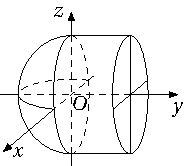
\includegraphics[scale=1]{figure/fig1-7-1.pdf}
			\caption{}\label{fig:1.7.1}
		\end{figure}
	\end{ti}

	\begin{ti}
		求曲面 $z = 2 \bigl( x^{2} + y^{2} \bigr), x^{2} + y^{2} = x, x^{2} + y^{2} = 2x$ 和 $z = 0$ 所围几何体的体积.
	\end{ti}

	\begin{ti}
		设 $f(x)$ 在 $[0,1]$ 上连续,试证:
		\[
			\int_{0}^{1} \dd{x} \int_{0}^{x} \dd{y} \int_{0}^{y} f(x) f(y) f(z) \dd{z} = \frac{1}{3!} \Biggl[ \int_{0}^{1} f(t) \dd{t} \Biggr]^{3}.
		\]
	\end{ti}

	\begin{ti}
		设球体 $x^{2} + y^{2} + z^{2} \leq 2az$(如图~\ref{fig:1.7.2})中任一点的密度与该点到坐标原点的距离成正比,求此球体的重心.
		\begin{figure}[htbp]
			\centering
			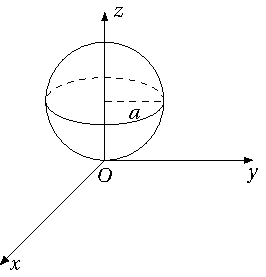
\includegraphics[scale=1]{figure/fig1-7-2.pdf}
			\caption{}\label{fig:1.7.2}
		\end{figure}
	\end{ti}

	\begin{ti}
		在密度为 $1$ 的半球体 $0 \leq z \leq \sqrt{R^{2} - x^{2} - y^{2}}$ 的底面接上一个相同材料的柱体:$-h \leq z < 0, x^{2} + y^{2} \leq R^{2} (h > 0)$,试确定 $h$ 值,使整个球柱体的重心恰好落在球心上.
	\end{ti}

	\begin{ti}
		设 $f(x)$ 为定义在 $[0,+\infty)$ 上的连续函数,且满足
		\[
			f(t) = \iiint_{\varOmega: x^{2} + y^{2} + z^{2} \leq t^{2}} f \Bigl( \sqrt{x^{2} + y^{2} + z^{2}} \Bigr) \dd{v} + t^{3},
		\]
		求 $f(1)$.
	\end{ti}
	\subsection{第一型曲线积分}

	\begin{ti}
		设 $L$ 为曲线 $\begin{cases}
			x^{2} + y^{2} + z^{2} = 9,\\
			x + y + z = 0,
		\end{cases}$ 则 $\int_{L} \bigl( 3x^{2} - y^{2} - z^{2} \bigr) \dd{s} = $\kuo.

		\fourch{$27\uppi$}{$18\uppi$}{$12\uppi$}{$6\uppi$}
	\end{ti}

	\begin{ti}
		计算 $I = \oint_{L} \ee^{\sqrt{x^{2} + y^{2}}} \dd{s}$,其中 $L$ 为由圆周 $x^{2} + y^{2} = a^{2}$ 及直线 $y = x$ 和 $y = 0$ 在第一象限内所围成的区域的边界.
	\end{ti}

	\begin{ti}
		求抛物柱面 $y = \sqrt{x}$ 被平面 $z = 0, z = y$ 和 $y = 1$ 所截部分的面积.
	\end{ti}

	\begin{ti}
		\begin{enumerate}
			\item 求函数
			\[
				f(x,y) = \begin{cases}
					\frac{x^{2}y}{x^{2} + y^{2}}, & x^{2} + y^{2} \ne 0,\\
					0, & x^{2} + y^{2} = 0
				\end{cases}
			\]
			的二阶偏导数 $f_{xy}''(0,0)$;
			\item 问微分方程 $\bigl( y^{2} + 6x \bigr)y' - 2y = 0$ 的哪一个解 $y = y(x)$ 满足条件 $x|_{y = 1} = f_{xy}''(0,0)$;
			\item 求曲线积分 $\int_{L} f(x,y) \dd{s}$,其中 $L$ 为 $x^{2} + y^{2} = 1$ 位于第一象限的部分.
		\end{enumerate}
	\end{ti}

	\begin{ti}
		设曲线 $\varGamma: x = a \cos t, y = a \sin t, z = bt(0 \leq t \leq 2\uppi)$,则 $\int_{\varGamma} \bigl( x^{2} + y^{2} \bigr) \dd{s} = $\htwo.
	\end{ti}

	\begin{ti}
		设某曲线 $L$ 的线密度 $\mu = x^{2} + y^{2} + z^{2}$,其方程为
		\[
			x = \ee^{t} \cos t, y = \ee^{t} \sin t, z = \sqrt{2} \ee^{t}, - \infty < t \leq 0.
		\]
		\begin{enumerate}
			\item 求曲线 $L$ 的弧长 $l$;
			\item 求曲线 $L$ 对 $z$ 轴的转动惯量 $J$;
			\item 求曲线 $L$ 对位于原点处质量为 $m$ 的质点的引力($k$ 为引力常数).
		\end{enumerate}
	\end{ti}
	\subsection{第一型曲面积分}

	\begin{ti}
		设 $\varSigma$ 是 $yOz$ 平面上的圆域 $y^{2} + z^{2} \leq 1$,则 $\iint_{\varSigma} \bigl( x^{2} + y^{2} + z^{2} \bigr) \dd{S} = $\kuo.

		\fourch{$0$}{$\uppi$}{$\frac{1}{4}\uppi$}{$\frac{1}{2}\uppi$}
	\end{ti}

	\begin{ti}
		设 $\varSigma$ 为球面 $(x - 1)^{2} + y^{2} + (z + 1)^{2} = 1$,则 $\iint_{\varSigma} (2x + 3y + z) \dd{S} = $\kuo.
		
		\fourch{$4\uppi$}{$2\uppi$}{$\uppi$}{$0$}
	\end{ti}

	\begin{ti}
		设 $S$ 为椭球面 $\frac{x^{2}}{9} + \frac{y^{2}}{4} + z^{2} = 1$,已知 $S$ 的面积为 $A$,则第一型曲面积分 $\iint_{S} \bigl[ (2x + 3y)^{2} + (6z - 1)^{2} \bigr] \dd{S} = $
		
		\noindent\htwo.
	\end{ti}

	\begin{ti}
		设 $S$ 为球面 $x^{2} + y^{2} + z^{2} = R^{2}$ 被锥面 $z = \sqrt{Ax^{2} + By^{2}}$ 截下的小的那部分,并设其中 $A, B, R$ 均为正常数且 $A \ne B$,则第一型曲面积分 $\iint_{S} z \dd{S} = $

		\noindent\htwo.
	\end{ti}

	\begin{ti}
		设 $\varSigma$ 是正圆锥面 $z = \sqrt{x^{2} + y^{2}} (0 \leq z \leq 1)$,则曲面积分 $\iint_{\varSigma} z \dd{S} = $\kuo.

		\fourch{$\frac{2\sqrt{2}}{3}\uppi$}{$\frac{\sqrt{2}}{3}\uppi$}{$\sqrt{2}\uppi$}{$\uppi$}
	\end{ti}

	\begin{ti}
		空间曲面 $z = xy$ 被圆柱体 $x^{2} + y^{2} \leq 1$ 所截部分的面积 $A = $\htwo.
	\end{ti}

	\begin{ti}
		设 $\varSigma$ 为球面:$x^{2} + y^{2} + z^{2} = 1$,则第一类曲面积分 $\iint_{\varSigma} x (4x - z) \dd{S} = $\htwo.
	\end{ti}

	\begin{ti}
		计算曲面积分 $I = \iint_{\varSigma} (ax + by + cz + d)^{2} \dd{S}$,其中 $\varSigma$ 是球面 $x^{2} + y^{2} + z^{2} = R^{2}$.
	\end{ti}

	\begin{ti}
		设 $\varSigma$ 为平面 $y + z = 5$ 被柱面 $x^{2} + y^{2} = 25$ 所截得的部分,计算曲面积分 $I = \iint_{\varSigma} (x + y + z) \dd{S}$.
	\end{ti}

	\begin{ti}
		计算 $\iint_{S} x^{2} \dd{S}$,其中 $S$ 为圆柱面 $x^{2} + y^{2} = a^{2}$ 介于 $z = 0$ 和 $z = h$ 之间的部分.
	\end{ti}

	\begin{ti}
		设半径为 $R$ 的球的球心位于以原点为中心、$a$ 为半径的定球面上($2a > R > 0$,$a$ 为常数). 试确定 $R$ 为何值时前者夹在定球面内部的表面积为最大,并求出此最大值.
	\end{ti}
	\subsection{第二型曲线积分}

	\begin{ti}
		设 $l$ 为自点 $O(0,0)$ 沿曲线 $y = \sin x$ 至点 $A(\uppi,0)$ 的有向弧段,求平面第二型曲线积分
		\[
			I = \int_{l} \bigl[ \ee^{x} \cos y + 2 (x + y) \bigr] \dd{x} + \Biggl( -\ee^{x} \sin y + \frac{3}{2}x \Biggr) \dd{y}.
		\]
	\end{ti}

	\begin{ti}
		设 $L$ 为圆周 $x^{2} + y^{2} = 4$ 正向一周,求
		\[
			I = \oint_{L} y^{3} \dd{x} + \bigl| 3y - x^{2} \bigr| \dd{y}.
		\]
	\end{ti}

	\begin{ti}
		计算曲线积分 $\oint_{L} \frac{y \dd{x} - x \dd{y}}{2\left(x^{2} + y^{2}\right)}$,其中 $L: (x - 1)^{2} + y^{2} = 2$,其方向为逆时针方向.
	\end{ti}

	\begin{ti}
		计算曲线积分 $\int_{C} \sqrt{x^{2} + y^{2}} \dd{x} + \bigl[ 2x + y\ln\bigl( x + \sqrt{x^{2} + y^{2}} \bigr) \bigr] \dd{y}$,其中有向曲线 $C: y = \sqrt{1 - \frac{(x - 3)^{2}}{4}}$,方向从点 $(5,0)$ 到点 $(1,0)$.
	\end{ti}

	\begin{ti}
		计算曲线积分
		\[
			\int_{L} \left( \frac{xy^{2}}{\sqrt{4 + x^{2}y^{2}}} + \frac{1}{\uppi}x \right)\dd{x} + \left( \frac{x^{2}y}{\sqrt{4 + x^{2}y^{2}}} - x + y \right)\dd{y},
		\]
		其中 $L$ 是摆线 $\begin{cases}
			x = a (t - \sin t),\\
			y = a (1 - \cos t)
		\end{cases} (a > 0)$ 上自 $O(0,0)$ 至 $A(2\uppi a,0)$ 的一段有向曲线弧.
	\end{ti}

	\begin{ti}
		计算曲线积分
		\[
			I = \int_{l} \bigl[ u_{x}'(x,y) + xy \bigr] \dd{x} + u_{y}'(x,y) \dd{y},
		\]
		其中 $l$ 是从点 $A(0,1)$ 沿曲线 $y = \frac{\sin x}{x}$ 到点 $B(\uppi,0)$ 的曲线段. $u(x,y)$ 在 $xOy$ 平面上具有二阶连续偏导数,且 $u(0,1) = 1$,$u(\uppi,0) = \uppi$.
	\end{ti}

	\begin{ti}
		设 $y' = f(x,y)$ 是一条简单封闭曲线 $L$(取正向),$f(x,y) \ne 0$,其所围区域记为 $D$,$D$ 的面积为 $1$,则 $I = \oint_{L} xf(x,y) \dd{x} - \frac{y}{f(x,y)} \dd{y} = $\htwo.
	\end{ti}

	\begin{ti}
		在过点 $O(0,0)$ 和 $A(\uppi,0)$ 的曲线族 $y = a \sin x$ $(a > 0)$ 中,求一条曲线 $L$,使沿该曲线从 $O$ 到 $A$ 的积分 $\int_{L} \bigl( 1 + y^{3} \bigr) \dd{x} + (2x + y) \dd{y}$ 的值最小.
	\end{ti}

	\begin{ti}
		证明
		\[
			\oint_{\varGamma} x f(y) \dd{y} - \frac{y}{f(x)} \dd{x} \geq 2\uppi,
		\]
		其中 $\varGamma$ 为圆周曲线 $(x - a)^{2} + (y - a)^{2} = 1 (a > 0)$ 正向,$f(x)$ 连续取正值.
	\end{ti}

	\begin{ti}
		设曲线积分 $\int_{L} \bigl[ f(x) - \ee^{x} \bigr] \sin y \dd{x} - f(x) \cos y \dd{y}$ 与路径无关,其中 $f(x)$ 具有一阶连续导数,且 $f(0) = 0$,则 $f(x)$ 等于\kuo.

		\twoch{$\frac{1}{2}\bigl( \ee^{-x} - \ee^{x} \bigr)$}{$\frac{1}{2}\bigl( \ee^{x} - \ee^{-x} \bigr)$}{$\frac{1}{2}\bigl( \ee^{x} + \ee^{-x} \bigr) - 1$}{$1 - \frac{1}{2}\bigl( \ee^{x} + \ee^{-x} \bigr)$}
	\end{ti}

	\begin{ti}
		已知曲线积分 $\int_{L} \bigl[ \ee^{x} \cos y + y f(x) \bigr] \dd{x} + \bigl( x^{3} - \ee^{x} \sin y \bigr) \dd{y}$ 与路径无关且 $f(x)$ 有连续的导数,则 $f(x) = $\htwo.
	\end{ti}

	\begin{ti}
		设 $f(x,y)$ 在全平面有连续偏导数,曲线积分 $\int_{L} f(x,y) \dd{x} + x \cos y \dd{y}$ 在全平面与路径无关,且 $\int_{(0,0)}^{\left(t,t^{2}\right)} f(x,y) \dd{x} + x \cos y \dd{y} = t^{2}$,求 $f(x,y)$.
	\end{ti}

	\begin{ti}
		设函数 $P(x,y) = \frac{x}{y}r^{\lambda}$,$Q(x,y) = - \frac{x^{2}}{y^{2}}r^{\lambda}$,其中 $r = \sqrt{x^{2} + y^{2}}$,若曲线积分 $\int_{L} P \dd{x} + Q \dd{y}$ 在区域 $D = \bigl\{ (x,y) \bigl| y > 0 \bigr\}$ 上与路径无关,求参数 $\lambda$.
	\end{ti}

	\begin{ti}
		设 $L$ 是摆线 $\begin{cases}
			x = t - \sin t - \uppi,\\
			y = 1 - \cos t
		\end{cases}$ 从 $t = 0$ 到 $t = 2\uppi$ 的一段,则 $\int_{L} \frac{(x - y)\dd{x} + (x + y) \dd{y}}{x^{2} + y^{2}} = $\kuo.
		
		\fourch{$-\uppi$}{$\uppi$}{$2\uppi$}{$-2\uppi$}
	\end{ti}

	\begin{ti}
		设函数 $g(x)$ 具有连续导数,曲线积分
		\[
			\int_{L} \bigl[ \ee^{2x} + g'(x) - 2g(x) \bigr]y \dd{x} - g'(x) \dd{y}
		\]
		与路径无关.
		\begin{enumerate}
			\item 求满足条件 $g(0) = -\frac{1}{4}, g'(0) = -\frac{1}{2}$ 的函数 $g(x)$;
			\item 计算 $\int_{(0,0)}^{(1,1)} \bigl[ \ee^{2x} + g'(x) - 2g(x) \bigr]y \dd{x} - g'(x) \dd{y}$ 的值.
		\end{enumerate}
	\end{ti}

	\begin{ti}
		微分方程 $\bigl( 2xy + \ee^{x}\sin y \bigr) \dd{x} + \bigl( x^{2} + \ee^{x} \cos y \bigr) \dd{y} = 0$ 的通解为\htwo.
	\end{ti}

	\begin{ti}
		\begin{enumerate}
			\item 设函数 $f(x)$ 具有一阶连续导数,且 $f(1) = 1$,$D$ 为不包含原点的单连通区域,在 $D$ 内曲线积分 $\int_{L} \frac{y\dd{x} - x\dd{y}}{2x^{2} + f(y)}$ 与路径无关,求 $f(y)$;\label{7.46:1}
			\item 在(\ref{7.46:1})的条件下,求 $\oint_{L'} \frac{y\dd{x} - x\dd{y}}{2x^{2} + f(y)}$,其中 $L'$ 为曲线 $x^{\frac{2}{3}} + y^{\frac{2}{3}} = a^{\frac{2}{3}}, a > 0$,且取逆时针方向.
		\end{enumerate}
	\end{ti}

	\begin{ti}
		设 $L$ 为曲线 $x^{2} + y^{2} = R^{2}$(常数 $R > 0$)一周,$\bm n$ 为 $L$ 的外法线方向向量,$u(x,y)$ 具有二阶连续偏导数且 $\frac{\partial^{2}u}{\partial x^{2}} + \frac{\partial^{2}u}{\partial y^{2}} = x^{2} + y^{2}$. 求 $\oint_{L} \frac{\partial u}{\partial \bm n} \dd{s}$.
	\end{ti}

	\begin{ti}
		计算 $\int_{\varGamma} y\dd{x} + z\dd{y} + x\dd{z}$,其中 $\varGamma$ 为螺旋线 $x = a \cos t, y = a \sin t, z = bt$ 从 $t = 0$ 到 $t = 2\uppi$ 的一段,如图~\ref{fig:1.7.3} 所示.
		\begin{figure}[htbp]
			\centering
			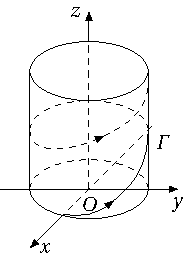
\includegraphics[scale=1]{figure/fig1-7-3.pdf}
			\caption{}\label{fig:1.7.3}
		\end{figure}
	\end{ti}
	\subsection{第二型曲面积分}

	\begin{ti}
		设 $\varSigma$ 是球面 $x^{2} + y^{2} + z^{2} = a^{2} (a > 0)$ 的外侧,则 $\oiint_{\varSigma} xy^{2} \dd{y}\dd{z} + yz^{2} \dd{z}\dd{x} + zx^{2} \dd{x}\dd{y} = $\htwo.
	\end{ti}

	\begin{ti}
		设 $\varSigma: x^{2} + y^{2} + z^{2} = 4 (z \geq 0)$,取上侧,试求曲面积分
		\[
			I = \iint_{\varSigma} \frac{x\dd{y}\dd{z} + y\dd{z}\dd{x} + z\dd{x}\dd{y}}{\sqrt{ x^{2} + (y - 1)^{2} + z^{2} }}.
		\]
	\end{ti}

	\begin{ti}
		设 $f(x,y,z)$ 为连续函数,$S$ 为曲面 $z = \frac{1}{2} \bigl( x^{2} + y^{2} \bigr)$ 介于 $z = 2$ 与 $z = 8$ 之间的上侧部分,求
		\begin{align*}
			\iint_{S} \bigl[ y f(x,y,z) + x \bigr] \dd{y} \dd{z} &+ \bigl[ x f(x,y,z) + y \bigr] \dd{z} \dd{x}\\
			&+ \bigl[ 2xy f(x,y,z) + z \bigr] \dd{x} \dd{y}.
		\end{align*}
	\end{ti}

	\begin{ti}
		设 $S$ 为平面 $x - y + z = 1$ 介于三坐标平面间的有限部分,法向量与 $z$ 轴交角为锐角,$f(x,y,z)$ 连续,计算
		\begin{align*}
			\iint_{S} \bigl[ f(x,y,z) + x \bigr] \dd{y} \dd{z} &+ \bigl[ 2f(x,y,z) + y \bigr] \dd{z} \dd{x}\\
			&+ \bigl[ f(x,y,z) + z \bigr] \dd{x} \dd{y}.
		\end{align*}
	\end{ti}

	\begin{ti}
		计算曲面积分
		\begin{align*}
			I = \iint_{\varSigma} \bigl( x^{3} + az^{2} \bigr) \dd{y} \dd{z} &+ \bigl( y^{3} + ax^{2} \bigr) \dd{z} \dd{x}\\
			&+ \bigl( z^{3} + ay^{2} \bigr) \dd{x} \dd{y},
		\end{align*}
		其中 $\varSigma$ 为上半球面 $z = \sqrt{a^{2} - x^{2} - y^{2}}$ 的上侧.
	\end{ti}

	\begin{ti}
		计算
		\[
			I = \oiint_{\varSigma} \frac{2 \dd{y} \dd{z}}{x \cos^{2}x} + \frac{\dd{z} \dd{x}}{\cos^{2}y} - \frac{\dd{x} \dd{y}}{z \cos^{2}z},
		\]
		其中 $\varSigma$ 为球面 $x^{2} + y^{2} + z^{2} = 1$ 的外侧.
	\end{ti}

	\begin{ti}
		设向量场
		\begin{align*}
			\bm F = \Biggl( x^{2} y z^{2}, \frac{1}{z} \arctan \frac{y}{z} - x y^{2} z^{2}, &\frac{1}{y} \arctan \frac{y}{z}\\
			&+ z(1 + xyz) \Biggr).
		\end{align*}
		\begin{enumerate}
			\item 计算 $\div \bm F |_{(1,1,1)}$ 的值;
			\item 设空间区域 $\varOmega$ 由锥面 $y^{2} + z^{2} = x^{2}$ 与球面 $x^{2} + y^{2} + z^{2} = a^{2}, x^{2} + y^{2} + z^{2} = 4 a^{2}$ 所围成 $(x > 0)$,其中 $a$ 为正常数,记 $\varOmega$ 表面的外侧为 $\varSigma$,计算积分
			\begin{align*}
				I =& \oiint_{\varSigma} x^{2} y z^{2} \dd{y} \dd{z} + \Biggl( \frac{1}{z} \arctan \frac{y}{z} - x y^{2} z^{2} \Biggr) \dd{z} \dd{x}\\
				&+ \Biggl[ \frac{1}{y} \arctan \frac{y}{z} + z(1 + xyz) \Biggr] \dd{x} \dd{y}.
			\end{align*}
		\end{enumerate}
	\end{ti}

	\begin{ti}
		设函数 $f(x,y,z)$ 在区域 $\varOmega = \bigl\{ (x,y,z) \bigl| x^{2} + y^{2} + z^{2} \leq 1 \bigr\}$ 上具有连续的二阶偏导数,且满足
		\[
			\frac{\partial^{2}f}{\partial x^{2}} + \frac{\partial^{2}f}{\partial y^{2}} + \frac{\partial^{2}f}{\partial z^{2}} = \sqrt{x^{2} + y^{2} + z^{2}},
		\]
		计算
		\[
			I = \iiint_{\varOmega} \Biggl( x \frac{\partial f}{\partial x} + y \frac{\partial f}{\partial y} + z \frac{\partial f}{\partial z} \Biggr) \dd{x} \dd{y} \dd{z}.
		\]
	\end{ti}

	\begin{ti}
		计算曲线积分 $I = \oint_{L} y^{2} \dd{x} + z^{2} \dd{y} + x^{2} \dd{z}$,其中曲线 $L$ 为 $\begin{cases}
			x^{2} + y^{2} + z^{2} = 4,\\
			x^{2} + y^{2} = 2x
		\end{cases} (z \geq 0)$,从 $x$ 轴的正向往负向看去,取逆时针方向.
	\end{ti}
	\subsection{场论}

	\begin{ti}
		已知 $\bm F = x^{3} \bm i + y^{3} \bm j + z^{3} \bm k$,则在点 $(1,0,-1)$ 处的 $\div \bm F$ 为\htwo.
	\end{ti}

	\begin{ti}
		设 $u = x^{2} + 3y + yz$,则 $\div \bigl(\grad u\bigr) = $\htwo.
	\end{ti}

	\begin{ti}
		向量场 $\bm A(z,3x,2y)$ 在点 $M(x,y,z)$ 处的旋度 $\rot \bm A = $\htwo.
	\end{ti}

	\begin{ti}
		函数
		\[
			u = 3x^{2}y - 2yz + z^{3}, v = 4xy - z^{3},
		\]
		点 $P(1,-1,1)$. $u$ 在点 $P$ 处沿 $\grad v \bigr|_{P}$ 方向的方向导数等于\htwo.
	\end{ti}

	\begin{ti}
		函数 $u = \ee^{z} - z + xy$ 在点 $(2,1,0)$ 处沿曲面 $\ee^{z} - z + xy = 3$ 的法线方向的方向导数为\htwo.
	\end{ti}

	\begin{ti}
		设 $\bm n$ 是曲面 $2x^{2} + 3y^{2} + z^{2} = 6$ 在点 $P(1,1,1)$ 处的指向外侧的法向量,求函数 $u = \frac{1}{z} \bigl( 6x^{2} + 8y^{2} \bigr)^{\frac{1}{2}}$ 在此处沿方向 $\bm n$ 的方向导数.
	\end{ti}

	\begin{ti}
		求函数 $f(x,y) = x^{2} - xy + y^{2}$ 在点 $M(1,1)$ 沿与 $x$ 轴的正向组成 $\alpha$ 角的方向 $\bm l$ 上的方向导数,在怎样的方向上此导数有:
		\begin{enumerate}
			\item 最大的值;
			\item 最小的值;
			\item 等于 $0$.
		\end{enumerate}
	\end{ti}

	\begin{ti}
		设在平面区域 $D$ 上数量场 $u(x,y) = 50 - x^{2} - 4y^{2}$,试问在点 $P_{0}(1,-2) \in D$ 处沿什么方向时 $u(x,y)$ 升高最快,并求一条路径,使从点 $P_{0}(1,-2)$ 处出发沿这条路径 $u(x,y)$ 升高最快.
	\end{ti}

	\begin{ti}
		求常数 $a,b,c$ 的值,使函数
		\[
			f(x,y,z) = axy^{2} + byz + cx^{3}z^{2}
		\]
		在点 $(1,2,-1)$ 处沿 $z$ 轴正向的方向导数有最大值 $64$.
	\end{ti}

	\begin{ti}
		设数量场 $u = x^{2} + 2y^{2} + 3z^{2} + xy + 3x - 2y - 6z$,求:
		\begin{enumerate}
			\item 梯度为零向量的点;
			\item 在点 $(2,0,1)$ 处,沿哪一个方向 $u$ 的变化率最大,并求此最大变化率;
			\item 使其梯度垂直于 $z$ 轴的点.
		\end{enumerate}
	\end{ti}
	\section{常微分方程}

	\begin{ti}
		微分方程 $3 \ee^{x} \tan y \dd{x} + \bigl( 1 - \ee^{x} \bigr) \sec^{2}y \dd{y} = 0$ 的通解是\htwo.
	\end{ti}

	\begin{ti}
		微分方程 $y' \tan x = y \ln y$ 的通解是\htwo.
	\end{ti}

	\begin{ti}
		已知曲线 $y = y(x)$ 经过点 $\bigl( 1,\ee^{-1} \bigr)$,且在点 $(x,y)$ 处的切线在 $y$ 轴上的截距为 $xy$,求该曲线方程的表达式.
	\end{ti}

	\begin{ti}
		求方程 $\frac{\dd{y}}{\dd{x}} = \bigl( 1 - y^{2} \bigr) \tan x$ 的通解以及满足 $y(0) = 2$ 的特解.
	\end{ti}

	\begin{ti}
		微分方程 $x \dd{y} = \bigl( y - \sqrt{x^{2} + y^{2}} \bigr) \dd{x}(x > 0)$ 满足 $y(1) = 0$ 的特解是\kuo.

		\twoch{$\sqrt{x^{2} + y^{2}} + y = x$}{$\sqrt{x^{2} + y^{2}} + y = 1$}{$\sqrt{x^{2} + y^{2}} - y = x$}{$\sqrt{x^{2} + y^{2}} - y = 1$}
	\end{ti}

	\begin{ti}
		求微分方程 $\bigl( 1 + \ee^{-\frac{x}{y}} \bigr) y \dd{x} + (y - x) \dd{y} = 0$ 的通解.
	\end{ti}

	\begin{ti}
		求微分方程 $xy' + y = x\ee^{x}$ 满足 $y(1) = 1$ 的特解.
	\end{ti}

	\begin{ti}
		求 $(4 - x + y) \dd{x} - (2 - x - y) \dd{y} = 0$ 的通解.
	\end{ti}

	\begin{ti}
		求微分方程 $\Bigl( x \frac{\dd{y}}{\dd{x}} - y \Bigr) \arctan \frac{y}{x} = x$ 的通解.
	\end{ti}

	\begin{ti}
		求微分方程 $\bigl( y + \sqrt{x^{2} + y^{2}} \bigr) \dd{x} = x \dd{y}$ 的通解,并求满足 $y(1) = 0$ 的特解.
	\end{ti}

	\begin{ti}
		微分方程 $\bigl( y^{2} + 1 \bigr) \dd{x} = y (y - 2x) \dd{y}$ 的通解是
		
		\noindent\htwo.
	\end{ti}

	\begin{ti}
		已知 $\int_{0}^{1} f(tx) \dd{t} = \frac{1}{2} f(x) + 1$,则 $f(x) = $\htwo.
	\end{ti}

	\begin{ti}
		设 $a > 0$,函数 $f(x)$ 在 $[0,+\infty)$ 内连续有界,证明:微分方程 $y' + ay = f(x)$ 的解在 $[0,+\infty)$ 内有界.
	\end{ti}

	\begin{ti}
		设 $\varphi(x)$ 是以 $2\uppi$ 为周期的连续函数,且 $\varPhi'(x) = \varphi(x), \varPhi(0) = 0$.
		\begin{enumerate}
			\item 求方程 $y' + y \sin x = \varphi(x) \ee^{\cos x}$ 的通解;\label{8.14:1}
			\item 在(\ref{8.14:1})中方程是否有以 $2\uppi$ 为周期的解?若有,请写出所需条件,若没有,请说明理由.
		\end{enumerate}
	\end{ti}

	\begin{ti}
		设方程 $y' + P(x)y = x^{2}$,其中 $P(x) = \begin{cases}
			1, & x \leq 1,\\
			\frac{1}{x}, & x > 1.
		\end{cases}$ 试求在 $(-\infty,+\infty)$ 内的连续函数 $y = y(x)$,使之在 $(-\infty,1)$ 和 $(1,+\infty)$ 内都满足方程,且满足初值条件 $y(0) = 2$.
	\end{ti}

	\begin{ti}
		微分方程 $\frac{\dd{y}}{\dd{x}} = \frac{2xy}{x^{2} + y}$ 的通解为\htwo.
	\end{ti}

	\begin{ti}
		求微分方程 $y' \cos y = (1 + \cos x \sin y)\sin y$ 的通解.
	\end{ti}

	\begin{ti}
		微分方程 $y'' - 6y' + 8y = \ee^{x} + \ee^{2x}$ 的一个特解应具有形式(其中 $a,b$ 为常数)\kuo.

		\twoch{$a \ee^{x} + b \ee^{2x}$}{$a \ee^{x} + b x \ee^{2x}$}{$a x \ee^{x} + b \ee^{2x}$}{$a x \ee^{x} + b x \ee^{2x}$}
	\end{ti}

	\begin{ti}
		微分方程 $y'' - 4y' + 4y = x^{2} + 8\ee^{2x}$ 的一个特解应具有形式(其中 $a,b,c,d$ 为常数)\kuo.

		\twoch{$ax^{2} + bx + c\ee^{2x}$}{$ax^{2} + bx + c + dx^{2}\ee^{2x}$}{$ax^{2} + bx + cx\ee^{2x}$}{$ax^{2} + \bigl(bx^{2} + cx\bigr)\ee^{2x}$}
	\end{ti}

	\begin{ti}
		微分方程 $y'' + y' + y = \ee^{-\frac{1}{2}x} \sin \frac{\sqrt{3}}{2} x$ 的一个特解应具有形式(其中 $a,b$ 为常数)\kuo.

		\onech{$\ee^{-\frac{1}{2}x} \Bigl( a \sin \frac{\sqrt{3}}{2}x + bx \cos \frac{\sqrt{3}}{2}x \Bigr)$}{$\ee^{-\frac{1}{2}x} \Bigl( a \cos \frac{\sqrt{3}}{2}x + b \sin \frac{\sqrt{3}}{2}x \Bigr)$}{$x\ee^{-\frac{1}{2}x} \Bigl( a \cos \frac{\sqrt{3}}{2}x + b \sin \frac{\sqrt{3}}{2}x \Bigr)$}{$\ee^{-\frac{1}{2}x} \Bigl( a \cos \frac{\sqrt{3}}{2}x + bx \sin \frac{\sqrt{3}}{2}x \Bigr)$}
	\end{ti}

	\begin{ti}
		设以下的 $A,B,C$ 为某些常数,微分方程 $y'' + 2y' - 3y = \ee^{x} \sin^{2}x$ 有特解形如\kuo.

		\onech{$\ee^{x} (A + B \cos 2x + C \sin 2x)$}{$\ee^{x} (Ax + B \cos 2x + C \sin 2x)$}{$\ee^{x} (A + B x \cos 2x + C x \sin 2x)$}{$x \ee^{x} (A + B \cos 2x + C \sin 2x)$}
	\end{ti}

	\begin{ti}
		求微分方程 $y'' - 2y' - \ee^{2x} = 0$ 满足条件 $y(0) = 1, y'(0) = 1$ 的特解.
	\end{ti}

	\begin{ti}
		求二阶常系数线性微分方程 $y'' + \lambda y' = 2x + 1$ 的通解,其中 $\lambda$ 为常数.
	\end{ti}

	\begin{ti}
		求微分方程 $y'' + 2y' + y = x\ee^{x}$ 的通解.
	\end{ti}

	\begin{ti}
		微分方程 $\frac{\dd^{2}y}{\dd{x^{2}}} + (x + \sin y) \Bigl( \frac{\dd{y}}{\dd{x}} \Bigr)^{3} = 0$ 满足初值条件 $y(0) = 0, y'(0) = \frac{2}{3}$ 的特解\htwo.
	\end{ti}

	\begin{ti}
		求一个以 $y_{1} = t \ee^{t}, y_{2} = \sin 2t$ 为两个特解的四阶常系数齐次线性微分方程,并求其通解.
	\end{ti}

	\begin{ti}
		设 $y(x)$ 是方程 $y^{(4)} - y'' = 0$ 的解,且当 $x \to 0$ 时,$y(x)$ 是 $x$ 的 $3$ 阶无穷小,求 $y(x)$.
	\end{ti}

	\begin{ti}
		设 $y_{1} = \ee^{x}, y_{2} = x^{2}$ 为某二阶齐次线性微分方程的两个特解,则该微分方程为\htwo.
	\end{ti}

	\begin{ti}
		设 $p(x), q(x)$ 与 $f(x)$ 均为连续函数,$f(x) \not\equiv 0$. 设 $y_{1}(x),y_{2}(x)$ 与 $y_{3}(x)$ 是二阶非齐次线性微分方程
		\begin{equation}\label{eq:8.29}
			y'' + p(x)y' + q(x)y = f(x)
		\end{equation}
		的 $3$ 个解,且
		\[
			\frac{y_{1} - y_{2}}{y_{2} - y_{3}} \ne \text{常数},
		\]
		则式~\eqref{eq:8.29} 的通解为\htwo.
	\end{ti}

	\begin{ti}
		求 $xy'' - y'\ln y' + y'\ln x = 0$ 满足 $y(1) = 2$ 和 $y'(1) = \ee^{2}$ 的特解.
	\end{ti}

	\begin{ti}
		求 $y'^{2} - yy'' = 1$ 的通解.
	\end{ti}

	\begin{ti}
		求 $(x + 2)y'' + xy'^{2} = y'$ 的通解.
	\end{ti}

	\begin{ti}
		求解 $y'' = \ee^{2y} + \ee^{y}$,且 $y(0) = 0,y'(0) = 2$.
	\end{ti}

	\begin{ti}
		微分方程 $y \dd{x} - x \dd{y} = x^{2} y \dd{y}$ 的通解为\htwo

		\noindent\htwo.
	\end{ti}

	\begin{ti}
		求 $\bigl( y^{3} - 3xy^{2} - 3x^{2}y \bigr) \dd{x} + \bigl( 3xy^{2} - 3x^{2}y - x^{3} + y^{2} \bigr) \dd{y} = 0$ 的通解.
	\end{ti}

	\begin{ti}
		求方程 $x^{2} \frac{\dd^{2}y}{\dd{x^{2}}} - 2y = x^{2}$ 的通解.
	\end{ti}

	\begin{ti}
		求解微分方程 $(1 + x)^{3} \frac{\dd^{3}y}{\dd{x^{3}}} - 3(1 + x)^{2} \frac{\dd^{2}y}{\dd{x^{2}}} + 6(1 + x) \frac{\dd{y}}{\dd{x}} - 6y = 0$.
	\end{ti}

	\begin{ti}
		\begin{enumerate}
			\item 用 $x = \ee^{t}$ 化简微分方程
			\[
				x^{2} \frac{\dd^{2}y}{\dd{x^{2}}} + 3x \frac{\dd{y}}{\dd{x}} + 5y = 16x \ln x
			\]
			为
			\[
				\frac{\dd^{2}y}{\dd{t^{2}}} + 2\frac{\dd{y}}{\dd{t}} + 5y = 16t \ee^{t};
			\]
			\item 求解 $\frac{\dd^{2}y}{\dd{t^{2}}} + 2\frac{\dd{y}}{\dd{t}} + 5y = 16t \ee^{t}$.
		\end{enumerate}
	\end{ti}

	\begin{ti}
		适当选取函数 $\varphi(x)$,作变量代换 $y = \varphi(x) u$,将 $y$ 关于 $x$ 的微分方程 $\frac{\dd^{2}y}{\dd{x^{2}}} + x \frac{\dd{y}}{\dd{x}} + \Bigl( \frac{1}{4}x^{2} + \frac{1}{2} \Bigr)y = 0$ 化为 $u$ 关于 $x$ 的二阶常系数线性齐次微分方程 $\frac{\dd^{2}u}{\dd{x^{2}}} + \lambda u = 0$,求 $\varphi(x)$ 及常数 $\lambda$,并求原方程满足 $y(0) = 1,y'(0) = 0$ 的特解.
	\end{ti}

	\begin{ti}
		已知 $y = f(x)$ 是微分方程 $xy' - y = \sqrt{2x - x^{2}}$ 满足初始条件 $f(1) = 0$ 的特解,则 $\int_{0}^{1} f(x) \dd{x} = $\htwo.
	\end{ti}

	\begin{ti}
		设 $f(x)$ 是以 $2\uppi$ 为周期的二阶可导函数,满足关系式 $f(x) + 2f'(x + \uppi) = \sin x$,求 $f(x)$.
	\end{ti}

	\begin{ti}
		设函数 $y(x) (x \geq 0)$ 二阶可导且 $y'(x) > 0, y(0) = 1$. 过曲线 $y = y(x)$ 上任意一点 $P(x,y)$ 作该曲线的切线及到 $x$ 轴的垂线,上述两直线与 $x$ 轴所围成的三角形的面积记为 $S_{1}$,区间 $[0,x]$ 上以 $y = y(x)$ 为曲边的曲边梯形面积记为 $S_{2}$,并设 $2S_{1} - S_{2}$ 恒为 $1$,求此曲线 $y = y(x)$ 的方程.
	\end{ti}

	\begin{ti}
		位于上半平面且图形凹的曲线 $y = y(x)$ 在点 $(0,1)$ 处的切线斜率为 $0$,在点 $(2,2)$ 处的切线斜率为 $1$. 已知曲线上任一点处的曲率半径与 $\sqrt{y}$ 及 $\bigl( 1 + y'^{2} \bigr)$ 的乘积成正比,求该曲线方程.
	\end{ti}

	\begin{ti}
		求一条凹曲线,已知其上任意一点处的曲率 $k = \frac{1}{2y^{2} \cos \alpha}$,其中 $\alpha$ 为该曲线在相应点处的切线的倾斜角($\cos\alpha > 0$),且该曲线在点 $(1,1)$ 处的切线为水平方向.
	\end{ti}

	\begin{ti}
		如图~\ref{fig:1.8.1} 所示,正圆柱形水桶中装满水,当打开水桶底部的水龙头时,随着水的流出,水面高度 $y$ 逐渐下降. 当水面高度 $y$ 较大时,水的流出速率较快; 当水面高度 $y$ 越来越小时,流出速率也越来越小. 假定水面高度 $y$ 的下降速率与 $y$ 的平方根成正比,即
		\begin{equation}\label{eq:8.45}
			\frac{\dd{y}}{\dd{t}} = - k \sqrt{y},
		\end{equation}
		其中 $k$ 为正的比例常数.
		\begin{figure}[htbp]
			\centering
			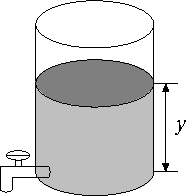
\includegraphics[scale=1]{figure/fig1-8-1.pdf}
			\caption{}\label{fig:1.8.1}
		\end{figure}
		\begin{enumerate}
			\item 求水面高度 $y$ 对于时间 $t$ 的函数 $y = y(t)$;
			\item 设 $k = \frac{1}{10}$. 当 $t = 0$ 时,$y = 9$. 需要多长时间水桶中的水才能流光?($t$ 的单位是 \si{min},$y$ 的单位是 \si{m})
		\end{enumerate}
	\end{ti}

	\begin{ti}
		正方体冰块放在空气中,其边长为 $m$,在温度恒定的情况下,冰块的融化速度(即体积减少速度)与冰块的表面积成正比,比例常数为 $k > 0$. 假设冰块在融化过程中始终保持正方体形状. 经过一个小时的融化,冰块的体积减小了四分之一. 求冰块完全融化需要的时间.
	\end{ti}
	\section{级数}
	\subsection{正项级数}

	\begin{ti}
		设 $f(x) = \int_{0}^{\sin x} \sin \bigl( t^{2} \bigr) \dd{t}, g(x) = \sum_{n=1}^{\infty} \frac{x^{2n+1}}{n^{n} + 2}$,则 $x \to 0$ 时,$f(x)$ 是 $g(x)$ 的\kuo 无穷小.

		\twoch{低阶}{同阶非等价}{等价}{高阶}
	\end{ti}

	\begin{ti}
		设正项级数 $\sum_{n=1}^{\infty} a_{n}$ 收敛,正项级数 $\sum_{n=1}^{\infty} b_{n}$ 发散,则
		
		\noindent\circled{1}~$\sum_{n=1}^{\infty} a_{n} b_{n}$ 必收敛;\\
		\circled{2}~$\sum_{n=1}^{\infty} a_{n} b_{n}$ 必发散;\\
		\circled{3}~$\sum_{n=1}^{\infty} a_{n}^{2}$ 必收敛;\\
		\circled{4}~$\sum_{n=1}^{\infty} b_{n}^{2}$ 必发散\\
		中结论正确的有\kuo.

		\fourch{$1$ 个}{$2$ 个}{$3$ 个}{$4$ 个}
	\end{ti}

	\begin{ti}
		当级数 $\sum_{n=1}^{\infty} a_{n}^{2},\sum_{n=1}^{\infty} b_{n}^{2}$ 都收敛时,级数 $\sum_{n=1}^{\infty} a_{n} b_{n}$\kuo.

		\onech{条件收敛}{绝对收敛}{发散}{可能收敛,也可能发散}
	\end{ti}

	\begin{ti}
		判别下列正项级数的敛散性:
		\begin{enumerate}
			\item $\sum_{n=1}^{\infty} \bigl( \frac{n}{3n + 2} \bigr)^{n}$;
			\item $\sum_{n=1}^{\infty} \int_{0}^{\frac{1}{n}} \frac{\sqrt{x}}{1 + x^{2}} \dd{x}$;
			\item $\sum_{n=1}^{\infty} \bigl( \sqrt[3]{n + 1} - \sqrt[3]{n} \bigr)$.
		\end{enumerate}
	\end{ti}

	\begin{ti}
		判别级数 $\sum_{n=1}^{\infty} \int_{0}^{\frac{\uppi}{n}} \frac{\sin x}{1 + x} \dd{x}$ 的敛散性.
	\end{ti}

	\begin{ti}
		设 $u_{n} = \int_{0}^{1} x (1 - x) \sin^{2n}x \dd{x}$,讨论级数 $\sum_{n=1}^{\infty} u_{n}$ 的敛散性.
	\end{ti}

	\begin{ti}
		设 $0 \leq u_{n} \leq \frac{1}{n}$,则下列级数中一定收敛的是\kuo.

		\twoch{$\sum_{n=1}^{\infty} u_{n}$}{$\sum_{n=1}^{\infty} (-1)^{n} u_{n}$}{$\sum_{n=1}^{\infty} \sqrt{u_{n}}$}{$\sum_{n=1}^{\infty} (-1)^{n} u_{n}^{2}$}
	\end{ti}

	\begin{ti}
		求 $\lim_{n \to \infty} \frac{1}{4^{n}} \bigl( 1 + \frac{1}{n} \bigr)^{n^{2}}$.
	\end{ti}

	\begin{ti}
		设 $\sum_{n=1}^{\infty} u_{n}$ 和 $\sum_{n=1}^{\infty} v_{n}$ 都是正项级数. 试证:
		\begin{enumerate}
			\item 若 $\sum_{n=1}^{\infty} u_{n}$ 收敛,则 $\sum_{n=1}^{\infty} \sqrt{u_{n} u_{n+1}}$ 收敛;
			\item 若 $\sum_{n=1}^{\infty} \sqrt{u_{n} u_{n+1}}$ 收敛,$u_{n}$ 单调减少,则 $\sum_{n=1}^{\infty} u_{n}$ 收敛;
			\item 若 $\sum_{n=1}^{\infty} v_{n}$ 和 $\sum_{n=1}^{\infty} u_{n}$ 都收敛,则 $\sum_{n=1}^{\infty} u_{n} v_{n}$ 收敛;
			\item 若 $\sum_{n=1}^{\infty} u_{n}$ 收敛,则 $\sum_{n=1}^{\infty} \frac{u_{n}}{n}$ 收敛. 
		\end{enumerate}
	\end{ti}

	\begin{ti}
		求 $\lim_{n \to \infty} \frac{n! a^{n}}{n^{n}}$($a$ 为常数,$0 < |a| < \ee$).
	\end{ti}

	\begin{ti}
		判别下列级数的敛散性($k > 1, a > 1$):
		\begin{enumerate}
			\item $\sum_{n=1}^{\infty} \frac{n^{k}}{a^{n}}$;
			\item $\sum_{n=1}^{\infty} \frac{a^{n}}{n!}$;
			\item $\sum_{n=1}^{\infty} \frac{n!}{n^{n}}$.
		\end{enumerate}
	\end{ti}

	\begin{ti}
		常数项级数 $\frac{1}{2} + \frac{1}{10} + \frac{1}{2^{2}} + \frac{1}{10 \times 2} + \cdots + \frac{1}{2^{n}} + \frac{1}{10n} + \cdots$ 的敛散性为\htwo.
	\end{ti}

	\begin{ti}
		\begin{enumerate}
			\item 设 $\sum_{n=1}^{\infty} u_{n}$ 为正项级数,证明:$\sum_{n=1}^{\infty} u_{n}$ 收敛的充要条件是其部分和数列 $\{ s_{n} \}$ 有界;
			\item 设 $\{ x_{n} \}$ 为单调递增的有界正数数列,证明:$\sum_{n=1}^{\infty} \Bigl( 1 - \frac{x_{n}}{x_{n+1}} \Bigr)$ 收敛.
		\end{enumerate}
	\end{ti}

	\begin{ti}
		设数列 $\{ a_{n} \}, \{ b_{n} \}$ 满足
		\[
			\ee^{b_{n}} = \ee^{a_{n}} - a_{n} (n = 1,2,3,\cdots),
		\]
		求证:
		\begin{enumerate}
			\item 若 $a_{n} > 0$,则 $b_{n} > 0$;
			\item 若 $a_{n} > 0(n = 1,2,3,\cdots), \sum_{n=1}^{\infty} a_{n}$ 收敛,则 $\sum_{n=1}^{\infty} \frac{b_{n}}{a_{n}}$ 收敛.
		\end{enumerate}
	\end{ti}
	\subsection{交错级数}

	\begin{ti}
		已知级数 $\sum_{n=1}^{\infty} (-1)^{n} n \sqrt{n} \tan \frac{1}{n^{\alpha}}$ 绝对收敛,级数 $\sum_{n=1}^{\infty} \frac{(-1)^{n}}{n^{3 - \alpha}}$ 条件收敛,则\kuo.
		
		\twoch{$0 < \alpha \leq \frac{1}{2}$}{$1 < \alpha < \frac{5}{2}$}{$1 < \alpha < 3$}{$\frac{5}{2} < \alpha < 3$}
	\end{ti}

	\begin{ti}
		设 $a_{n} = \cos n \uppi \cdot \ln \Big( 1 + \frac{1}{\sqrt{n}} \Bigr) (n = 1,2,3,\cdots)$,则级数\kuo.

		\onech{$\sum_{n=1}^{\infty} a_{n}$ 与 $\sum_{n=1}^{\infty} a_{n}^{2}$ 都收敛}{$\sum_{n=1}^{\infty} a_{n}$ 与 $\sum_{n=1}^{\infty} a_{n}^{2}$ 都发散}{$\sum_{n=1}^{\infty} a_{n}$ 收敛,$\sum_{n=1}^{\infty} a_{n}^{2}$ 发散}{$\sum_{n=1}^{\infty} a_{n}$ 发散,$\sum_{n=1}^{\infty} a_{n}^{2}$ 收敛}
	\end{ti}

	\begin{ti}
		设 $f(x)$ 在区间 $[0,1]$ 上连续,且 $0 \leq f(x) \leq 1$,又设 $a_{n} = \int_{0}^{\frac{1}{n}} \sqrt{1 + f^{n}(x)} \dd{x}$,则级数 $\sum_{n=1}^{\infty} (-1)^{n} a_{n}$\kuo.

		\onech{发散}{条件收敛}{绝对收敛}{敛散性与具体的 $f(x)$ 有关}
	\end{ti}

	\begin{ti}
		设 $a > 0$ 为常数,则 $\sum_{n=1}^{\infty} (-1)^{n} \Bigl( 1 - \cos \frac{a}{n} \Bigr)$\kuo.

		\twoch{绝对收敛}{条件收敛}{发散}{敛散性与 $a$ 有关}
	\end{ti}

	\begin{ti}
		级数 $\sum_{n=1}^{\infty} (-1)^{n-1} \ln \Bigl( 1 + \frac{1}{n} \Bigr)$\kuo.

		\twoch{收敛}{发散}{条件收敛}{绝对收敛}
	\end{ti}

	\begin{ti}
		判别级数 $\sum_{n=1}^{\infty} \sin \bigl( \uppi \sqrt{n^{2} + a^{2}} \bigr)$ 的敛散性.
	\end{ti}

	\begin{ti}
		判别级数 $\sum_{n=2}^{\infty} \ln \Bigl[ 1 + \frac{(-1)^{n}}{\sqrt{n}} \Bigr]$ 的敛散性.
	\end{ti}

	\begin{ti}
		判别级数 $\sum_{n=2}^{\infty} \frac{(-1)^{n}}{\sqrt{n} + (-1)^{n}}$ 的敛散性.
	\end{ti}

	\begin{ti}
		证明:级数 $\sum_{n=2}^{\infty} \frac{(-1)^{n}}{\sqrt{n + (-1)^{n}}}$ 条件收敛.
	\end{ti}
	\subsection{综合}

	\begin{ti}
		设级数 $\sum_{n=1}^{\infty} a_{n}$ 收敛,则\kuo.

		\onech{$\sum_{n=1}^{\infty} a_{n}^{2}$ 必收敛}{$\sum_{n=1}^{\infty} \frac{(-1)^{n}}{n} a_{n}$ 必收敛}{$\sum_{n=1}^{\infty} (a_{n} + a_{n+1})$ 必收敛}{$\sum_{n=1}^{\infty} a_{n} a_{n+1}$ 必收敛}
	\end{ti}

	\begin{ti}
		下列命题中正确的是\kuo.

		\onech{若 $u_{n} < v_{n} (n = 1,2,3,\cdots)$,则 $\sum_{n=1}^{\infty} u_{n} \leq \sum_{n=1}^{\infty} v_{n}$}{若 $u_{n} < v_{n} (n = 1,2,3,\cdots), \sum_{n=1}^{\infty} v_{n}$ 收敛,则 $\sum_{n=1}^{\infty} u_{n}$ 收敛}{若 $\lim_{n \to \infty} \frac{u_{n}}{v_{n}} = 1, \sum_{n=1}^{\infty} v_{n}$ 收敛,则 $\sum_{n=1}^{\infty} u_{n}$ 收敛}{若 $w_{n} < u_{n} < v_{n} (n = 1,2,3,\cdots), \sum_{n=1}^{\infty} w_{n}$ 与 $\sum_{n=1}^{\infty} v_{n}$ 收敛,则 $\sum_{n=1}^{\infty} u_{n}$ 收敛}
	\end{ti}

	\begin{ti}
		设 $f(x)$ 在区间 $(0,1)$ 内可导,且导函数 $f'(x)$ 有界,证明:
		\begin{enumerate}
			\item 级数 $\sum_{n=2}^{\infty} \bigl[ f \bigl( \frac{1}{n} \bigr) - f \bigl( \frac{1}{n + 1} \bigr) \bigr]$ 绝对收敛;
			\item $\lim_{n \to \infty} f \bigl( \frac{1}{n} \bigr)$ 存在.
		\end{enumerate}
	\end{ti}

	\begin{ti}
		设 $a$ 为正数,若级数 $\sum_{n=1}^{\infty} \frac{a^{n} n!}{n^{n}}$ 收敛,而
		\[
			\sum_{n=2}^{\infty} \frac{\sqrt{n + 2} - \sqrt{n - 2}}{n^{a}}
		\]
		发散,则\kuo.

		\twoch{$a \leq \frac{1}{2}$}{$\frac{1}{2} < a < \ee$}{$a > \ee$}{$a = \ee$}
	\end{ti}

	\begin{ti}
		设函数 $f(x)$ 在区间 $(-\infty,+\infty)$ 上的可导函数,$|f'(x)| < k f(x)$,其中 $0 < k < 1$. 任取实数 $a_{0}$,定义 $a_{n} = \ln f (a_{n-1}), n = 1,2,\cdots$,证明:$\sum_{n=1}^{\infty} (a_{n} - a_{n-1})$ 绝对收敛.
	\end{ti}
	\section{求收敛半径、收敛域,阿贝尔定理}

	\begin{ti}
		若 $\sum_{n=1}^{\infty} a_{n} (x - 1)^{n}$ 在 $x = -1$ 处收敛,则在 $x = 2$ 处是\kuo.

		\twoch{条件收敛}{绝对收敛}{发散}{敛散性不确定}
	\end{ti}

	\begin{ti}
		若 $\sum_{n=0}^{\infty} a_{n} x^{n}$ 在 $x = -3$ 处为条件收敛,则其收敛半径 $R = $\htwo.
	\end{ti}

	\begin{ti}
		幂级数 $\sum_{n=1}^{\infty} \frac{1}{\sqrt{n}} (x - 2)^{n}$ 的收敛域为\htwo.
	\end{ti}

	\begin{ti}
		幂级数 $\sum_{n=1}^{\infty} (-1)^{n} \frac{x^{2n+1}}{2n+1}$ 的收敛域为\htwo.
	\end{ti}

	\begin{ti}
		设 $a_{n} = \frac{2^{n}}{(5^{n} + 2^{n})n}$,求幂级数 $\sum_{n=1}^{\infty} a_{n} x^{n}$ 的收敛半径、收敛区间与收敛域.
	\end{ti}
	\subsection{级数展开与求和}

	\begin{ti}
		函数 $f(x) = \frac{1}{x}$ 展开成的 $x - 1$ 的幂级数为\htwo.
	\end{ti}

	\begin{ti}
		$\ee^{x}$ 展开成的 $x - 3$ 的幂级数为\htwo.
	\end{ti}

	\begin{ti}
		将函数 $f(x) = \frac{1}{x^{2} - 3x + 2}$ 展开成 $x$ 的幂级数,并指出其收敛区间.
	\end{ti}

	\begin{ti}
		将 $y = \sin x$ 展开为 $x - \frac{\uppi}{4}$ 的幂级数.
	\end{ti}

	\begin{ti}
		将 $f(x) = \frac{1}{x^{2}}$ 展开为 $x + 1$ 的幂级数.
	\end{ti}

	\begin{ti}
		设 $f(x) = \frac{1}{1 - 2x - x^{2}}$.
		\begin{enumerate}
			\item 将 $f(x)$ 展开为 $x$ 的幂级数;
			\item 分别判断级数 $\sum_{n=0}^{\infty} \frac{n!}{f^{(n)}(0)}, \sum_{n=0}^{\infty} \frac{f^{(n)}(0)}{n!}$ 的敛散性.
		\end{enumerate}
	\end{ti}

	\begin{ti}
		将函数 $f(x) = \ln \bigl| \frac{x}{x - 3} \bigr|$ 展开成 $x - 2$ 的幂级数,并求出其收敛范围.
	\end{ti}

	\begin{ti}
		\begin{enumerate}
			\item 证明 $\sum_{n=1}^{\infty} (-1)^{n-1} \frac{1}{3n - 2} = \int_{0}^{1} \frac{1}{1 + x^{3}} \dd{x}$;
			\item 求 $\sum_{n=1}^{\infty} (-1)^{n-1} \frac{1}{3n - 2}$.
		\end{enumerate}
	\end{ti}

	\begin{ti}
		\begin{enumerate}
			\item 设 $f(x)$ 为任意阶可导函数,且
			\[
				f(x) = \sum_{n=0}^{\infty} a_{n} x^{n},
			\]
			若 $f(x)$ 为奇函数,证明
			\[
				f(x) = \sum_{n=1}^{\infty} a_{2n-1} x^{2n-1};
			\]
			\item 将函数 $f(x) = \int_{0}^{x} \ee^{x^{2} - t^{2}} \dd{t}$ 展开为 $x$ 的幂级数.
		\end{enumerate}
	\end{ti}

	\begin{ti}
		设函数 $f(x) = \frac{7 + 2x}{2 - x - x^{2}}$,当 $-1 < x < 1$ 时,其幂级数展开式为 $f(x) = \sum_{n=0}^{\infty} a_{n} x^{n}$.
		\begin{enumerate}
			\item 求 $a_{n} (n = 0,1,2,\cdots)$;
			\item 求级数 $\sum_{n=0}^{\infty} \frac{a_{n+1} - a_{n}}{(a_{n} - 2) (a_{n+1} - 2)}$ 的和.
		\end{enumerate}
	\end{ti}

	\begin{ti}
		级数 $\sum_{n=0}^{\infty} \frac{(\ln 3)^{n}}{2^{n}}$ 的和为\htwo.
	\end{ti}

	\begin{ti}
		当 $|x| < 1$ 时,级数 $\sum_{n=1}^{\infty} \frac{1}{n} x^{n}$ 的和函数是\kuo.

		\twoch{$\ln(1 - x)$}{$\ln \frac{1}{1 - x}$}{$\ln(x - 1)$}{$- \ln (x - 1)$}
	\end{ti}

	\begin{ti}
		幂级数 $\frac{1}{a} + \frac{2x}{a^{2}} + \cdots + \frac{nx^{n-1}}{a^{n}} + \cdots$ 在收敛区间 $(-a,a)$ 内的和函数 $S(x)$ 为\htwo.
	\end{ti}

	\begin{ti}
		求幂级数 $\sum_{n=0}^{\infty} \frac{(-1)^{n}}{3n + 1} x^{3n}$ 的收敛域与和函数,并求 $\sum_{n=0}^{\infty} \frac{(-1)^{n}}{3n + 1}$ 的和.
	\end{ti}

	\begin{ti}
		已知 $f_{n}(x)$ 满足 $f_{n}'(x) = f_{n}(x) + x^{n-1} \ee^{x}$($n$ 为正整数),且 $f_{n}(1) = \frac{\ee}{n}$,求函数项级数 $\sum_{n=1}^{\infty} f_{n}(x)$ 的和函数.
	\end{ti}

	\begin{ti}
		\begin{enumerate}
			\item 求函数项级数 $\ee^{-x} + 2 \ee^{-2x} + \cdots + n \ee^{-nx} + \cdots$ 收敛时 $x$ 的取值范围;
			\item 当上述级数收敛时,求其和函数 $S(x)$,并求
			\[
				\int_{\ln 2}^{\ln 3} S(x) \dd{x}.
			\]
		\end{enumerate}
	\end{ti}

	\begin{ti}
		求级数 $\sum_{n=2}^{\infty} \frac{x^{n-2}}{n \cdot 3^{n}}$ 的收敛域及其和函数.
	\end{ti}

	\begin{ti}
		求数项级数 $\sum_{n=1}^{\infty} (-1)^{n} \frac{n(n + 1)}{2^{n}}$ 的和.
	\end{ti}

	\begin{ti}
		设 $x_{1} = r > 0, x_{n+1} = x_{n} + x_{n}^{3}, n = 1,2,3,\cdots$. 则数项级数 $\sum_{n=1}^{\infty} \frac{x_{n}}{1 + x_{n}^{2}} = $\htwo.
	\end{ti}

	\begin{ti}
		求级数 $\sum_{n=0}^{\infty} \frac{x^{2n}}{(2n)!}$ 的和函数.
	\end{ti}

	\begin{ti}
		求数列 $\{ a_{n} \}$ 满足 $a_{1} = a_{2} = 1$,且 $a_{n+1} = a_{n} + a_{n-1}, n = 2,3,\cdots$. 证明在 $|x| < \frac{1}{2}$ 时幂级数 $\sum_{n=1}^{\infty} a_{n} x^{n-1}$ 收敛,并求其和函数与系数 $a_{n}$.
	\end{ti}

	\begin{ti}
		$\sum_{n=1}^{\infty} (-1)^{n-1} \frac{2n^{2}}{(2n)!} \frac{1}{2^{n}}$ 的和为\htwo.
	\end{ti}

	\begin{ti}
		已知 $y(x) = 2 + \sum_{n=1}^{\infty} \frac{x^{2n}}{(2n)!}$ 在 $(-\infty,+\infty)$ 是微分方程 $y'' - y = a$ 的解.
		\begin{enumerate}
			\item 求常数 $a$;
			\item 求 $y(x)$.
		\end{enumerate}
	\end{ti}

	\begin{ti}
		设 $y = f(x)$ 由方程组 $\begin{cases}
			x = \sum_{n=1}^{\infty} \frac{(t - 1)^{n}}{n},\\
			y = \sum_{n=1}^{\infty} \frac{n t^{n-1}}{2^{n}}
		\end{cases}$ 所确定,求 $\frac{\dd{y}}{\dd{x}}\bigr|_{t = 1}$.
	\end{ti}

	\begin{ti}
		设 $A_{n}$ 是曲线 $y = x^{n}$ 与 $y = x^{n+1}(n = 1,2,\cdots)$ 所围区域的面积,记 $S_{1} = \sum_{n=1}^{\infty} A_{n}, S_{2} = \sum_{n=1}^{\infty} A_{2n-1}$,求 $S_{1}$ 与 $S_{2}$ 的值.
	\end{ti}

	\begin{ti}
		已知 $\sum_{n=1}^{\infty} \frac{1}{n^{2}} = \frac{\uppi^{2}}{6}$.
		\begin{enumerate}
			\item 设 $f(x) = \sum_{n=1}^{\infty} \frac{1}{n^{2}} x^{n}$,证明当 $0 < x < 1$ 时,$f(x) + f(1 - x) + \ln x \ln (1 - x) = \frac{\uppi^{2}}{6}$;
			\item 求 $I = \int_{0}^{1} \frac{1}{2 - x} \ln \frac{1}{x} \dd{x}$.
		\end{enumerate}
	\end{ti}
	\subsection{傅氏级数}

	\begin{ti}
		设 $f(x) = x + 1 (0 \leq x \leq 1)$,则它以 $2$ 为周期的余弦级数在 $x = 0$ 处收敛于\kuo.

		\fourch{$1$}{$-1$}{$0$}{$\frac{1}{2}$}
	\end{ti}

	\begin{ti}
		若将 $f(x) = \begin{cases}
			x^{2}, & 0 \leq x \leq 1,\\
			0, & 1 \leq x \leq 2
		\end{cases}$ 在 $[0,2]$ 上展开成正弦级数,则该级数的和函数 $S(x)$ 为\htwo.
	\end{ti}

	\begin{ti}
		设 $f(x) = \begin{cases}
			x^{2}, & - \uppi \leq x < 0,\\
			-5, & 0 \leq x < \uppi,
		\end{cases}$ 则其以 $2 \uppi$ 为周期的傅里叶级数在 $x = \pm \uppi$ 处收敛于\htwo.
	\end{ti}

	\begin{ti}
		设 $f(x) = x^{2} (0 < x < 1)$,而
		\[
			S(x) = \sum_{n=1}^{\infty} b_{n} \sin n \uppi x, x \in (-\infty,+\infty),
		\]
		其中
		\[
			b_{n} = 2 \int_{0}^{1} f(x) \cdot \sin n \uppi x \dd{x}, n = 1,2,3,\cdots.
		\]
		则 $S\big( - \frac{1}{2} \bigr) = $\kuo.

		\fourch{$-\frac{1}{4}$}{$\frac{1}{4}$}{$-\frac{1}{2}$}{$\frac{1}{2}$}
	\end{ti}

	\begin{ti}
		设 $f(x) = \begin{cases}
			-1, & -\uppi < x \leq 0,\\
			1 + x^{2}, & 0 < x \leq \uppi,
		\end{cases}$ 则其以 $2\uppi$ 为周期的傅里叶级数在 $x = \uppi$ 处收敛于\htwo.
	\end{ti}

	\begin{ti}
		设 $f(x) = \uppi x + x^{2}, -\uppi \leq x < \uppi$,且周期为 $T = 2\uppi$. 若 $f(x)$ 在 $[-\uppi,\uppi)$ 上的傅里叶级数为
		\[
			\frac{a_{0}}{2} + \sum_{n=1}^{\infty} (a_{n} \cos nx + b_{n} \sin nx),
		\]
		则 $b_{3} = $\htwo.
	\end{ti}

	\begin{ti}
		函数 $f(x) = \begin{cases}
			-1, & -\uppi \leq x < 0,\\
			1, & 0 \leq x \leq \uppi
		\end{cases}$ 在 $[-\uppi,\uppi]$ 上展开为傅里叶级数 $\frac{a_{0}}{2} + \sum_{n=1}^{\infty} (a_{n} \cos nx + b_{n} \sin nx)$,则 $a_{n} = $\htwo,$b_{n} = $\htwo,和函数 $S(x) = $\htwo.
	\end{ti}

	\begin{ti}
		设 $f(x)$ 在区间 $[-\uppi,\uppi]$ 上连续且满足 $f(x + \uppi) = - f(x)$,则 $f(x)$ 的傅里叶系数 $a_{2n} = $\htwo.
	\end{ti}

	\begin{ti}
		设函数 $f(x)$ 是以 $2 \uppi$ 为周期的周期函数,且 $f(x) = \ee^{\alpha x} (0 \leq x < 2\uppi)$,其中 $\alpha \ne 0$,试将 $f(x)$ 展开成傅里叶级数,并求级数 $\sum_{n=1}^{\infty} \frac{1}{1 + n^{2}}$ 的和.
	\end{ti}

	\begin{ti}
		设
		\[
			f(x) = \begin{cases}
				x + 1, & 0 \leq x \leq \uppi,\\
				0, & - \uppi \leq x < 0,
			\end{cases}
		\]
		$S(x) = \frac{a_{0}}{2} + \sum_{n=1}^{\infty} (a_{n} \cos nx + b_{n} \sin nx)$ 是 $f(x)$ 的以 $2 \uppi$ 为周期的傅里叶级数,则 $\sum_{n = 1}^{\infty} (-1)^{n} a_{n} = $\htwo.
	\end{ti}

	\begin{ti}
		将函数 $f(x) = x^{2} (0 \leq x \leq \uppi)$ 展开成余弦级数,并求 $\sum_{n = 1}^{\infty} \frac{1}{n^{2}}$ 的和.
	\end{ti}
	% \ctexset{
	section={
		format={\zihao{4}\bfseries\raggedright},
		name={,、},
		aftername={\hspace{0em}},
		number=\chinese{section},
	},
}
\chapter{线性代数}
	线性代数是硕士研究生招生考试考查内容之一,主要考查考生对线性代数的基本概念基本理论、基本运算的理解和掌握以及考生的抽象思维能力、逻辑推理能力、空间想象能力、综合运用能力和解决实际问题的能力。在考研数学一试卷中分值为 $34$ 分,约占 $22\%$。
% \section{线性代数}
	\section{行列式}

	\begin{titwo}
		设 $\begin{vsmallmatrix}
			a_{11} & a_{12} & a_{13} & a_{14}\\
			a_{21} & a_{22} & a_{23} & a_{24}\\
			a_{31} & a_{32} & a_{33} & a_{34}\\
			a_{41} & a_{42} & a_{43} & a_{44}
		\end{vsmallmatrix} = m, c \ne 0$,则 
		\[
			\begin{vsmallmatrix}
				a_{11} & a_{12}c & a_{13}c^{2} & a_{14}c^{3}\\
				a_{21}c^{-1} & a_{22} & a_{23}c & a_{24}c^{2}\\
				a_{31}c^{-2} & a_{32}c^{-1} & a_{33} & a_{34}c\\
				a_{41}c^{-3} & a_{42}c^{-2} & a_{43}c^{-1} & a_{44}
			\end{vsmallmatrix}
		\]
		等于\kuo.

		\fourch{$c^{-2}m$}{$m$}{$cm$}{$c^{3}m$}
	\end{titwo}

	\begin{titwo}
		$\begin{vsmallmatrix}
			a & b & c & d \\
			x & 0 & 0 & y \\
			y & 0 & 0 & x \\
			d & c & b & a
		\end{vsmallmatrix} = $\htwo.
	\end{titwo}

	\begin{titwo}
		设 $a, b, a + b$ 均非零,则行列式 $\begin{vsmallmatrix}
			a & b & a + b \\
			b & a + b & a \\
			a + b & a & b \\
		\end{vsmallmatrix} = $
		
		\noindent\htwo.
	\end{titwo}

	\begin{titwo}
		设 $n$ 阶矩阵 $\bm A = \begin{bsmallmatrix}
			0 & 1 & 1 & \cdots & 1 & 1 \\
			1 & 0 & 1 & \cdots & 1 & 1 \\
			1 & 1 & 0 & \cdots & 1 & 1 \\
			\vdots & \vdots & \vdots &  & \vdots & \vdots \\
			1 & 1 & 1 & \cdots & 0 & 1 \\
			1 & 1 & 1 & \cdots & 1 & 0 
		\end{bsmallmatrix}$,则 $|\bm A| = $\htwo.
	\end{titwo}

	\begin{titwo}
		计算 $n$ 阶行列式 $\begin{bsmallmatrix}
			a & b & 0 & \cdots & 0 & 0 \\
			0 & a & b & \cdots & 0 & 0 \\
			0 & 0 & a & \cdots & 0 & 0 \\
			\vdots & \vdots & \vdots &  & \vdots & \vdots \\
			0 & 0 & 0 & \cdots & a & b \\
			b & 0 & 0 & \cdots & 0 & a 
		\end{bsmallmatrix}$.
	\end{titwo}

	\begin{titwo}
		计算行列式 $\begin{vsmallmatrix}
			x + 1 & x & x & \cdots & x \\
			x & x + \frac{1}{2} & x & \cdots & x \\
			x & x & x + \frac{1}{3} & \cdots & x \\
			\vdots & \vdots & \vdots &  & \vdots \\
			x & x & x & \cdots & x + \frac{1}{n}
		\end{vsmallmatrix}$.
	\end{titwo}

	\begin{titwo}
		计算行列式 $\begin{vsmallmatrix}
			1 - x & x & 0 & 0 & 0 \\
			-1 & 1 - x & x & 0 & 0 \\
			0 & -1 & 1 - x & x & 0 \\
			0 & 0 & -1 & 1 - x & x \\
			0 & 0 & 0 & -1 & 1 - x
		\end{vsmallmatrix}$.
	\end{titwo}

	\begin{titwo}
		计算行列式 $\begin{vsmallmatrix}
			a & b & c & d \\
			-b & a & -d & c \\
			-c & d & a & -b \\
			-d & -c & b & a \\
		\end{vsmallmatrix}$.
	\end{titwo}

	\begin{titwo}
		行列式 $D_{n+1} = \begin{vsmallmatrix}
			a^{n} & (a + 1)^{n} & \cdots & (a + n)^{n} \\
			a^{n - 1} & (a + 1)^{n - 1} & \cdots & (a + n)^{n - 1} \\
			\vdots & \vdots &  & \vdots \\
			a & a + 1 & \cdots & a + n \\
			1 & 1 & \cdots & 1
		\end{vsmallmatrix} = $\htwo.
	\end{titwo}

	\begin{titwo}
		设 $n$ 阶行列式
		\[
			D_{n} = \begin{vsmallmatrix}
				2 & 1 & 0 & \cdots & 0 & 0 \\
				1 & 2 & 1 & \cdots & 0 & 0 \\
				0 & 1 & 2 & \cdots & 0 & 0 \\
				\vdots & \vdots & \vdots &  & \vdots & \vdots \\
				0 & 0 & 0 & \cdots & 2 & 1 \\
				0 & 0 & 0 & \cdots & 1 & 2
			\end{vsmallmatrix},
		\]
		则 $\sum_{i=1}^{n} D_{i} = $\htwo.
	\end{titwo}

	\begin{titwo}
		设 $D_{n} = \begin{vsmallmatrix}
			a + 2 & 2a & 0 & \cdots & 0 & 0 \\
			1 & a + 2 & 2a & \cdots & 0 & 0 \\
			0 & 1 & a + 2 & \cdots & 0 & 0 \\
			\vdots & \vdots & \vdots &  & \vdots & \vdots \\
			0 & 0 & 0 & \cdots & a + 2 & 2a \\
			0 & 0 & 0 & \cdots & 1 & a + 2 
		\end{vsmallmatrix}$,其中 $n \geq 3$.

		\noindent 则 $\frac{D_{n} - a D_{n - 1}}{D_{n - 1} - a D_{n - 2}} = $\htwo.
	\end{titwo}

	\begin{titwo}
		设 $\bm \alpha_{1},\bm \alpha_{2},\bm \alpha_{3},\bm \beta_{1},\bm \beta_{2}$ 都是 $4$ 维列向量,且 $4$ 阶行列式 $\bigl|\bm \alpha_{1},\bm \alpha_{2},\bm \alpha_{3},\bm \beta_{1}\bigr| = m,\bigl|\bm \alpha_{1},\bm \alpha_{2},\bm \beta_{2},\bm \alpha_{3}\bigr| = n$,则 $4$ 阶行列式 $\bigl|\bm \alpha_{3},\bm \alpha_{2},\bm \alpha_{1},\bm \beta_{1} + \bm \beta_{2}\bigr|$ 等于\kuo.

		\fourch{$m + n$}{$- (m + n)$}{$n - m$}{$m - n$}
	\end{titwo}

	\begin{titwo}
		设 $\bm A = [\bm \alpha_{1},\bm \alpha_{2},\bm \alpha_{3}]$ 是 $3$ 阶矩阵,且 $|\bm A| = 4$,若
		\[
			\bm B = [\bm \alpha_{1} - 3 \bm \alpha_{2} + 2 \bm \alpha_{3}, \bm \alpha_{2} - 2 \bm \alpha_{3}, 2 \bm \alpha_{2} + \bm \alpha_{3}],
		\]
		则 $|\bm B| = $\htwo.
	\end{titwo}

	\begin{titwo}
		设 $\bm A$ 是 $m$ 阶矩阵,$\bm B$ 是 $n$ 阶矩阵,且
		\[
			|\bm A| = a, |\bm B| = b, \bm C = \begin{bsmallmatrix}
				\bm O & \bm A \\
				\bm B & \bm O
			\end{bsmallmatrix},
		\]
		则 $|\bm C| = $\htwo.
	\end{titwo}

	\begin{titwo}
		设 $\bm A$ 为奇数阶矩阵,且 $\bm A \bm A^{\TT} = \bm A^{\TT} \bm A = \bm E, |\bm A| > 0$,则 $|\bm A - \bm E| = $\htwo.
	\end{titwo}

	\begin{titwo}
		设 $\bm A$ 是 $n$ 阶矩阵,满足 $\bm A \bm A^{\TT} = \bm E$($\bm E$ 是 $n$ 阶单位矩阵,$\bm A^{\TT}$ 是 $\bm A$ 的转置矩阵),且 $|\bm A| < 0$,求 $|\bm A + \bm E|$.
	\end{titwo}
\subsection{矩阵}

	\begin{titwo}
		设 $n$ 维行向量 $\bm \alpha = \bigl[ \frac{1}{2}, 0 , \cdots , 0 , \frac{1}{2} \bigr]$,矩阵 $\bm A = \bm E - \bm \alpha^{\TT} \bm \alpha, \bm B = \bm E + 2 \bm \alpha^{\TT} \bm \alpha$,则 $\bm A \bm B = $\kuo.

		\fourch{$\bm O$}{$- \bm E$}{$\bm E$}{$\bm E + \bm \alpha^{\TT} \bm \alpha$}
	\end{titwo}

	\begin{titwo}
		已知 $\bm A, \bm B, \bm A + \bm B, \bm A^{-1} + \bm B^{-1}$ 均为 $n$ 阶可逆矩阵,则 $\bigl( \bm A^{-1} + \bm B^{-1} \bigr)^{-1}$ 等于\kuo.

		\twoch{$\bm A + \bm B$}{$\bm A^{-1} + \bm B^{-1}$}{$\bm A(\bm A + \bm B)^{-1} \bm B$}{$(\bm A + \bm B)^{-1}$}
	\end{titwo}

	\begin{titwo}
		设 $\bm A$ 是 $n$ 阶方阵,且 $\bm A^{3} = \bm O$,则\kuo.

		\onech{$\bm A$ 不可逆,且 $\bm E - \bm A$ 不可逆}{$\bm A$ 可逆,但 $\bm E + \bm A$ 不可逆}{$\bm A^{2} - \bm A + \bm E$ 及 $\bm A^{2} + \bm A + \bm E$ 均可逆}{$\bm A$ 不可逆,且必有 $\bm A^{2} = \bm O$}
	\end{titwo}

	\begin{titwo}
		设 $\bm A$ 为 $n$ 阶可逆矩阵,则下列等式中,不一定成立的是\kuo.

		\onech{$\bigl( \bm A + \bm A^{-1} \bigr)^{2} = \bm A^{2} + 2 \bm A \bm A^{-1} + \bigl( \bm A^{-1} \bigr)^{2}$}{$\bigl( \bm A + \bm A^{\TT} \bigr)^{2} = \bm A^{2} + 2 \bm A \bm A^{\TT} + \bigl( \bm A^{\TT} \bigr)^{2}$}{$\bigl( \bm A + \bm A^{\astt} \bigr)^{2} = \bm A^{2} + 2 \bm A \bm A^{\astt} + \bigl( \bm A^{\astt} \bigr)^{2}$}{$\bigl( \bm A + \bm E \bigr)^{2} = \bm A^{2} + 2 \bm A \bm E + \bm E^{2}$}
	\end{titwo}

	\begin{titwo}
		设 $\bm A = \begin{bsmallmatrix}
			0 & 1 & 1 & 1 \\
			1 & 0 & 1 & 1 \\
			1 & 1 & 0 & 1 \\
			1 & 1 & 1 & 0
		\end{bsmallmatrix}$,则 $\bm A^{-1}=$\htwo.
	\end{titwo}

	\begin{titwo}
		设 $\bm B = \begin{bsmallmatrix}
			0 & b_{1} & 0 & \cdots & 0 \\
			0 & 0 & b_{2} & \cdots & 0 \\
			\vdots & \vdots & \vdots &  & \vdots \\
			0 & 0 & 0 & \cdots & b_{n-1} \\
			b_{n} & 0 & 0 & \cdots & 0
		\end{bsmallmatrix}$,则 $\bm B^{-1} = $\htwo.
	\end{titwo}

	\begin{titwo}
		设 $\bm B = 2 \bm A - \bm E$,证明:$\bm B^{2} = \bm E$ 的充分必要条件是 $\bm A^{2} = \bm A$.
	\end{titwo}

	\begin{titwo}
		设 $\bm A = \begin{bsmallmatrix}
			a & b \\
			c & d
		\end{bsmallmatrix}$.
		\begin{enumerate}
			\item 计算 $\bm A^{2}$,并将 $\bm A^{2}$ 用 $\bm A$ 和 $\bm E$ 线性表出;
			\item 证明:当 $k > 2$ 时,$\bm A^{k} = \bm O$ 的充分必要条件为 $\bm A^{2} = \bm O$.
		\end{enumerate}
	\end{titwo}

	\begin{titwo}
		设 $\bm M = \begin{bsmallmatrix}
			\bm A & \bm B \\
			\bm O & \bm D
		\end{bsmallmatrix}$ 可逆,其中 $\bm A, \bm D$ 皆为方阵,证明 $\bm A, \bm D$ 可逆,并求 $\bm M^{-1}$.
	\end{titwo}

	\begin{titwo}
		设 $\bm A$ 为 $n$ 阶非奇异矩阵,$\bm \alpha$ 为 $n$ 维列向量,$b$ 为常数. 记分块矩阵
		\[
			\bm P = \begin{bsmallmatrix}
				\bm E & \bm 0 \\
				- \bm \alpha^{\TT} \bm A^{\astt} & |\bm A|
			\end{bsmallmatrix},
			\bm Q = \begin{bsmallmatrix}
				\bm A & \bm \alpha \\
				\bm \alpha^{\TT} & b
			\end{bsmallmatrix},
		\]
		其中 $\bm A^{\astt}$ 是矩阵 $\bm A$ 的伴随矩阵,$\bm E$ 为 $n$ 阶单位矩阵.
		\begin{enumerate}
			\item 计算并化简 $\bm P \bm Q$;
			\item 证明:矩阵 $\bm Q$ 可逆的充分必要条件是 $\bm \alpha^{\TT} \bm A^{-1} \bm \alpha \ne b$.
		\end{enumerate}
	\end{titwo}

	\begin{titwo}
		已知 $\bm A$ 是 $n$ 阶方阵,$\bm E$ 是 $n$ 阶单位矩阵,且
		\[
			\bm A^{3} = \bm E,
		\]
		则 $\begin{bsmallmatrix}
			\bm O & - \bm E \\
			\bm A & \bm O
		\end{bsmallmatrix}^{98} = $\kuo.

		\fourch{$\begin{bsmallmatrix}
			\bm A & \bm E \\
			\bm O & \bm A
		\end{bsmallmatrix}$}{$\begin{bsmallmatrix}
			\bm A & \bm O \\
			\bm E & \bm A
		\end{bsmallmatrix}$}{$\begin{bsmallmatrix}
			\bm A & \bm O \\
			\bm O & \bm A
		\end{bsmallmatrix}$}{$\begin{bsmallmatrix}
			- \bm A & \bm O \\
			\bm O & - \bm A
		\end{bsmallmatrix}$}
	\end{titwo}

	\begin{titwo}
		下列命题正确的是\kuo.

		\onech{若 $\bm A \bm B = \bm E$,则 $\bm A$ 必可逆,且 $\bm A^{-1} = \bm B$}{若 $\bm A, \bm B$ 均为 $n$ 阶可逆矩阵,则 $\bm A + \bm B$ 必可逆}{若 $\bm A, \bm B$ 均为 $n$ 阶不可逆矩阵,则 $\bm A - \bm B$ 必不可逆}{若 $\bm A, \bm B$ 均为 $n$ 阶不可逆矩阵,则 $\bm A \bm B$ 必不可逆}
	\end{titwo}

	\begin{titwo}
		设 $\bm A$ 为 $3$ 阶非零矩阵,且满足
		\[
			a_{ij} = A_{ij} (i,j = 1,2,3),
		\]
		其中 $A_{ij}$ 为 $a_{ij}$ 的代数余子式,则下列结论中:\circled{1} $\bm A$ 是可逆矩阵; \circled{2} $\bm A$ 是对称矩阵; \circled{3} $\bm A$ 是不可逆矩阵; \circled{4} $\bm A$ 是正交矩阵. 正确的个数为\kuo.

		\fourch{$1$}{$2$}{$3$}{$4$}
	\end{titwo}

	\begin{titwo}
		设 $n$ 阶矩阵 $\bm A, \bm B$ 等价,则下列说法中,不一定成立的是\kuo.

		\onech{如果 $|\bm A| > 0$,则 $|\bm B| > 0$}{如果 $\bm A$ 可逆,则存在可逆矩阵 $\bm P$,使得 $\bm P \bm B = \bm E$}{如果 $\bm A, \bm E$ 等价,则 $|\bm B| \ne 0$}{存在可逆矩阵 $\bm P$ 与 $\bm Q$,使得 $\bm P \bm A \bm Q = \bm B$}
	\end{titwo}

	\begin{titwo}
		设 $\bm A = \begin{bsmallmatrix}
			1 & 0 & 0 & 0 \\
			-2 & 3 & 0 & 0 \\
			0 & -4 & 5 & 0 \\
			0 & 0 & -6 & 7 \\
		\end{bsmallmatrix}, \bm B = (\bm E + \bm A)^{-1} (\bm E - \bm A)$,则 $(\bm E + \bm B)^{-1} = $\htwo.
	\end{titwo}

	\begin{titwo}
		设
		\[
			\bm B = \begin{bsmallmatrix}
				0 & 1 & 0 & 0 \\
				0 & 0 & 1 & 0 \\
				0 & 0 & 0 & 1 \\
				0 & 0 & 0 & 0
			\end{bsmallmatrix},
		\]
		证明 $\bm A = \bm E + \bm B$ 可逆,并求 $\bm A^{-1}$.
	\end{titwo}

	\begin{titwo}
		证明:方阵 $\bm A$ 与所有同阶对角矩阵可交换的充分必要条件是 $\bm A$ 是对角矩阵.
	\end{titwo}

	\begin{titwo}
		设 $\bm \alpha, \bm \beta$ 为 $n$ 维单位列向量,$\bm P$ 是 $n$ 阶可逆矩阵,则下列矩阵中可逆的是\kuo.

		\twoch{$\bm A = \bm E - \bm \alpha \bm \alpha^{\TT}$}{$\bm B = \bm \alpha^{\TT} \bm P \bm \alpha \bm P^{-1} - \bm \alpha \bm \alpha^{\TT}$}{$\bm C = \bm \alpha^{\TT} \bm P^{-1} \bm \beta \bm P - \bm \beta \bm \alpha^{\TT}$}{$\bm D = \bm E + \bm \beta \bm \beta^{\TT}$}
	\end{titwo}

	\begin{titwo}
		设 $\bm A$ 是 $m \times n$ 矩阵,$\bm B$ 是 $n \times m$ 矩阵,已知 $\bm E_{m} + \bm A \bm B$ 可逆.
		\begin{enumerate}
			\item 验证 $\bm E_{n} + \bm B \bm A$ 可逆,且
			\[
				(\bm E_{n} + \bm B \bm A)^{-1} = \bm E_{n} - \bm B (\bm E_{m} + \bm A \bm B)^{-1} \bm A;
			\]
			\item 设 $\bm W = \begin{bsmallmatrix}
				1 + a_{1} b_{1} & a_{1} b_{2} & a_{1} b_{3} \\
				a_{2} b_{1} & 1 + a_{2} b_{2} & a_{2} b_{3} \\
				a_{3} b_{1} & a_{3} b_{2} & 1 + a_{3} b_{3}
			\end{bsmallmatrix}$,其中 $a_{1} b_{1} + a_{2} b_{2} + a_{3} b_{3} = 0$. 证明:$\bm W$ 可逆,并求 $\bm W^{-1}$.
		\end{enumerate}
	\end{titwo}

	\begin{titwo}
		设
		\[
			\bm \alpha = [1,2,3], \bm \beta = \Biggl[ 1,\frac{1}{2},\frac{1}{3} \Biggr], \bm A = \bm \alpha^{\TT} \bm \beta,
		\]
		则 $\bm A^{n} = $\htwo.
	\end{titwo}

	\begin{titwo}
		设 $\bm A = \begin{bsmallmatrix}
			1 & 2 & 3 \\
			0 & 1 & 4 \\
			0 & 0 & 1
		\end{bsmallmatrix}$,求 $\bm A^{n} (n \geq 3)$.
	\end{titwo}

	\begin{titwo}
		设
		\[
			\bm A = \begin{bsmallmatrix}
				1 & 0 & 1 \\
				0 & 2 & 0 \\
				1 & 0 & 1
			\end{bsmallmatrix},
		\]
		$n \geq 2$ 为正整数,则 $\bm A^{n} - 2 \bm A^{n-1} = $\htwo.
	\end{titwo}

	\begin{titwo}
		设 $\bm A = \begin{bsmallmatrix}
			1 & 0 & 0 \\
			1 & 0 & 1 \\
			0 & 1 & 0
		\end{bsmallmatrix}$.
		\begin{enumerate}
			\item 证明当 $n \geq 3$ 时,有 $\bm A^{n} = \bm A^{n-2} + \bm A^{2} - \bm E$;
			\item 求 $\bm A^{100}$.
		\end{enumerate}
	\end{titwo}

	\begin{titwo}
		已知 $\bm A = \begin{bsmallmatrix}
			3 & 1 & 0 & 0 & 0 \\
			0 & 3 & 1 & 0 & 0 \\
			0 & 0 & 3 & 0 & 0 \\
			0 & 0 & 0 & 3 & -1 \\
			0 & 0 & 0 & -9 & 3
		\end{bsmallmatrix}$,求 $\bm A^{n}(n \geq 2)$.
	\end{titwo}

	\begin{titwo}
		设 $\bm \alpha = [a_{1},a_{2},\cdots,a_{n}]^{\TT} \ne \bm 0, \beta = [b_{1},b_{2},\cdots,b_{n}]^{\TT} \ne \bm 0$,且 $\bm \alpha^{\TT} \bm \beta = 0, \bm A = \bm E + \bm \alpha \bm \beta^{\TT}$,试计算:
		\begin{enumerate}
			\item $|\bm A|$;
			\item $\bm A^{n}$;
			\item $\bm A^{-1}$.
		\end{enumerate}
	\end{titwo}

	\begin{titwo}
		设 $\bm A$ 是 $n(n \geq 2)$ 阶方阵,$\bm A^{\astt}$ 是 $\bm A$ 的伴随矩阵,则 $|\bm A^{\astt}| = $\kuo.

		\fourch{$|\bm A|$}{$|\bm A^{-1}|$}{$|\bm A^{n-1}|$}{$|\bm A^{n}|$}
	\end{titwo}

	\begin{titwo}
		设 $\bm A$ 是 $n(n \geq 2)$ 阶方阵,$|\bm A| = 3$,则 $|( A^{\astt} )^{\astt}| = $
		
		\noindent\kuo.

		\fourch{$3^{(n-1)^{2}}$}{$3^{n^{2} - 1}$}{$3^{n^{2} - n}$}{$3^{n-1}$}
	\end{titwo}

	\begin{titwo}
		设 $\bm A$ 是 $n(n \geq 2)$ 阶可逆方阵,$\bm A^{\astt}$ 是 $\bm A$ 的伴随矩阵,则 $(\bm A^{\astt})^{\astt} = $\kuo.

		\fourch{$|\bm A|^{n-1} \bm A$}{$|\bm A|^{n+1} \bm A$}{$|\bm A|^{n-2} \bm A$}{$|\bm A|^{n+2} \bm A$}
	\end{titwo}

	\begin{titwo}
		设 $\bm A_{n \times n}$ 是正交矩阵,则\kuo.

		\twoch{$\bm A^{\astt} (\bm A^{\astt})^{\TT} = |\bm A| \bm E$}{$(\bm A^{\astt})^{\TT} \bm A^{\astt} = |\bm A^{\astt}| \bm E$}{$\bm A^{\astt} (\bm A^{\astt})^{\TT} = \bm E$}{$(\bm A^{\astt})^{\TT} \bm A^{\astt} = - \bm E$}
	\end{titwo}

	\begin{titwo}
		设 $\bm A = \frac{1}{2} \begin{bsmallmatrix}
			2 & 0 & 0 \\
			0 & 0 & 1 \\
			0 & 3 & 0
		\end{bsmallmatrix}$,则 $(\bm A^{\astt})^{-1} = $\htwo.
	\end{titwo}

	\begin{titwo}
		证明:若 $\bm A$ 为 $n$ 阶可逆方阵,$\bm A^{\astt}$ 为 $\bm A$ 的伴随矩阵,则 $(\bm A^{\astt})^{\TT} = \bigl( \bm A^{\TT} \bigr)^{\astt}$.
	\end{titwo}

	\begin{titwo}
		证明:若 $\bm A$ 为 $n(n \geq 2)$ 阶方阵,则有
		\[
			|\bm A^{\astt}| = |(- \bm A)^{\astt}|.
		\]
	\end{titwo}

	\begin{titwo}
		设 $\bm A$ 是 $n$ 阶矩阵,则 $\left| -2 \begin{bsmallmatrix}
			\bm A^{\astt} & \bm O \\
			\bm A + \bm A^{\astt} & \bm A
		\end{bsmallmatrix} \right| = $\kuo.

		\twoch{$(-2)^{n} |\bm A|^{n}$}{$(4 |\bm A|)^{n}$}{$(-2)^{2n} |\bm A^{\astt}|^{n}$}{$|4 \bm A|^{n}$}
	\end{titwo}

	\begin{titwo}
		设 $\bm A$ 是 $n$ 阶矩阵,$|\bm A| = 5$,则 $|( 2 \bm A )^{\astt}| = $\htwo.
	\end{titwo}

	\begin{titwo}
		$|\bm A|$ 是 $n$ 阶行列式,其中有一行(列)元素全是 $1$,证明:这个行列式的全部代数余子式的和等于该行列式的值.
	\end{titwo}

	\begin{titwo}
		$\bm A$ 为 $n(n \geq 3)$ 阶非零实矩阵,$A_{ij}$ 为 $|\bm A|$ 中元素 $a_{ij}$ 的代数余子式,试证明:
		\begin{enumerate}
			\item $a_{ij} = A_{ij} \Leftrightarrow \bm A^{\TT} \bm A = \bm E$,且 $|\bm A| = 1$;
			\item $a_{ij} = -A_{ij} \Leftrightarrow \bm A^{\TT} \bm A = \bm E$,且 $|\bm A| = -1$.
		\end{enumerate}
	\end{titwo}

	\begin{titwo}
		设 $\bm A = \begin{bsmallmatrix}
			1 & 2 & 3 & 4 \\
			0 & 1 & 2 & 3 \\
			0 & 0 & 1 & 2 \\
			0 & 0 & 0 & 1
		\end{bsmallmatrix}$,求 $|\bm A|$ 的所有代数余子式之和.
	\end{titwo}

	\begin{titwo}
		证明:$n > 3$ 的非零实方阵 $\bm A$,若它的每个元素等于自己的代数余子式,则 $\bm A$ 是正交矩阵.
	\end{titwo}

	\begin{titwo}
		已知 $\bm A, \bm B$ 均是 $3$ 阶矩阵,将 $\bm A$ 中第 $3$ 行的 $-2$ 倍加到第 $2$ 行得矩阵 $\bm A_{1}$,将 $\bm B$ 中第 $1$ 列和第 $2$ 列对换得到 $\bm B_{1}$,又 $\bm A_{1} \bm B_{1} = \begin{bsmallmatrix}
			1 & 1 & 1 \\
			1 & 0 & 2 \\
			2 & 1 & 3
		\end{bsmallmatrix}$,则 $\bm A \bm B = $\htwo.
	\end{titwo}

	\begin{titwo}
		已知 $\bm A = \begin{bsmallmatrix}
			0 & 1 & 0 \\
			1 & 0 & 0 \\
			0 & 0 & 1
		\end{bsmallmatrix}^{5} \begin{bsmallmatrix}
			1 & 0 & 0 \\
			0 & 5 & 0 \\
			0 & 0 & 3
		\end{bsmallmatrix} \begin{bsmallmatrix}
			1 & 0 & 0 \\
			0 & 1 & 1 \\
			0 & 0 & 1
		\end{bsmallmatrix}^{4}$,则 $\bm A^{-1} = $\htwo.
	\end{titwo}

	\begin{titwo}
		设 $\bm A$ 是 $n$ 阶可逆矩阵,将 $\bm A$ 的第 $i$ 行和第 $j$ 行对换得到的矩阵记为 $\bm B$. 证明 $\bm B$ 可逆,并推导 $\bm A^{-1}$ 和 $\bm B^{-1}$ 的关系.
	\end{titwo}

	\begin{titwo}
		设
		\begin{gather*}
			\bm A = \begin{bsmallmatrix}
				a_{11} & a_{12} & a_{13} \\
				a_{21} & a_{22} & a_{23} \\
				a_{31} & a_{32} & a_{33}
			\end{bsmallmatrix},
			\bm B = \begin{bsmallmatrix}
				a_{21} & a_{22} & a_{23} \\
				a_{11} & a_{12} & a_{13} \\
				a_{31} + a_{11} & a_{32} + a_{12} & a_{33} + a_{13}
			\end{bsmallmatrix}, \\
			\bm P_{1} = \begin{bsmallmatrix}
				0 & 1 & 0 \\
				1 & 0 & 0 \\
				0 & 0 & 1
			\end{bsmallmatrix},
			\bm P_{2} = \begin{bsmallmatrix}
				1 & 0 & 0 \\
				0 & 1 & 0 \\
				1 & 0 & 1
			\end{bsmallmatrix},
		\end{gather*}
		则必有\kuo.
		
		\twoch{$\bm A \bm P_{1} \bm P_{2} = \bm B$}{$\bm A \bm P_{2} \bm P_{1} = \bm B$}{$\bm P_{1} \bm P_{2} \bm A = \bm B$}{$\bm P_{2} \bm P_{1} \bm A = \bm B$}
	\end{titwo}

	\begin{titwo}
		设
		\begin{gather*}
			\bm A = \begin{bsmallmatrix}
				a_{11} & a_{12} & a_{13} & a_{14} \\
				a_{21} & a_{22} & a_{23} & a_{24} \\
				a_{31} & a_{32} & a_{33} & a_{34} \\
				a_{41} & a_{42} & a_{43} & a_{44}
			\end{bsmallmatrix},
			\bm B = \begin{bsmallmatrix}
				a_{14} & a_{13} & a_{12} & a_{11} \\
				a_{24} & a_{23} & a_{22} & a_{21} \\
				a_{34} & a_{33} & a_{32} & a_{31} \\
				a_{44} & a_{43} & a_{42} & a_{41}
			\end{bsmallmatrix}, \\
			\bm P_{1} = \begin{bsmallmatrix}
				0 & 0 & 0 & 1 \\
				0 & 1 & 0 & 0 \\
				0 & 0 & 1 & 0 \\
				1 & 0 & 0 & 0
			\end{bsmallmatrix},
			\bm P_{2} = \begin{bsmallmatrix}
				1 & 0 & 0 & 0 \\
				0 & 0 & 1 & 0 \\
				0 & 1 & 0 & 0 \\
				0 & 0 & 0 & 1
			\end{bsmallmatrix}.
		\end{gather*}
		其中 $\bm A$ 可逆,则 $\bm B^{-1}$ 等于\kuo.

		\twoch{$\bm A^{-1} \bm P_{1} \bm P_{2}$}{$\bm P_{1} \bm A^{-1} \bm P_{2}$}{$\bm P_{1} \bm P_{2} \bm A^{-1}$}{$\bm P_{2} \bm A^{-1} \bm P_{1}$}
	\end{titwo}

	\begin{titwo}
		设 $\bm A, \bm B$ 是 $n$ 阶方阵,则下列结论正确的是
		
		\noindent\kuo.

		\onech{$\bm A \bm B = \bm O \Leftrightarrow \bm A = \bm O $ 或 $\bm B = \bm O$}{$|\bm A| = 0 \Leftrightarrow \bm A = \bm O$}{$|\bm A \bm B| = 0 \Leftrightarrow |\bm A| = 0$ 或 $|\bm B| = 0$}{$\bm A = \bm E \Leftrightarrow |\bm A| = 1$}
	\end{titwo}

	\begin{titwo}
		已知 $n$ 阶方阵 $\bm A$ 满足矩阵方程 $\bm A^{2} - 3 \bm A - 2 \bm E = \bm O$. 证明 $\bm A$ 可逆,并求出其逆矩阵 $\bm A^{-1}$.
	\end{titwo}

	\begin{titwo}
		已知对于 $n$ 阶方阵 $\bm A$,存在自然数 $k$,使得 $\bm A^{k} = \bm O$. 证明矩阵 $\bm E - \bm A$ 可逆,并写出其逆矩阵的表达式($\bm E$ 为 $n$ 阶单位矩阵).
	\end{titwo}

	\begin{titwo}
		设矩阵 $\bm A = \begin{bsmallmatrix}
			1 & 0 & 1 \\
			0 & 2 & 0 \\
			1 & 0 & 1
		\end{bsmallmatrix}$,矩阵 $\bm X$ 满足 $\bm A \bm X + \bm E = \bm A^{2} + \bm X$,其中 $\bm E$ 为 $3$ 阶单位矩阵. 求矩阵 $\bm X$.
	\end{titwo}

	\begin{titwo}
		设 $\bm A, \bm B$ 均是 $n$ 阶矩阵,且 $\bm A \bm B = \bm A + \bm B$. 证明 $\bm A - \bm E$ 可逆,并求 $(\bm A - \bm E)^{-1}$.
	\end{titwo}

	\begin{titwo}
		已知 $\bm A, \bm B$ 是 $3$ 阶方阵,$\bm A \ne \bm O, \bm A \bm B = \bm O$,证明:$\bm B$ 不可逆.
	\end{titwo}

	\begin{titwo}
		设 $\bm A, \bm B$ 均为 $n$ 阶矩阵,且 $\bm A \bm B = \bm A + \bm B$,则下列命题中:

		{\raggedright
		\begin{tabular}{l}
			\circled{1} 若 $\bm A$ 可逆,则 $\bm B$ 可逆;\\
			\circled{2} 若 $\bm A + \bm B$ 可逆,则 $\bm B$ 可逆;\\
			\circled{3} 若 $\bm B$ 可逆,则 $\bm A + \bm B$ 可逆;\\
			\circled{4} $\bm A - \bm E$ 恒可逆.
		\end{tabular}}

		\noindent 正确的个数为\kuo.

		\fourch{$1$}{$2$}{$3$}{$4$}
	\end{titwo}

	\begin{titwo}
		设 $3$ 阶方阵 $\bm A, \bm B$ 满足关系式 $\bm A^{-1} \bm B \bm A = 6 \bm A + \bm B \bm A$,且 $\bm A = \begin{bsmallmatrix}
			\frac{1}{3} & 0 & 0 \\
			0 & \frac{1}{4} & 0 \\
			0 & 0 & \frac{1}{7}
		\end{bsmallmatrix}$,则 $\bm B = $\htwo.
	\end{titwo}

	\begin{titwo}
		已知 $\bm A^{2} - 2 \bm A + \bm E = \bm O$,则 $(\bm A + \bm E)^{-1} = $\htwo.
	\end{titwo}

	\begin{titwo}
		设 $\bigl( 2 \bm E - \bm C^{-1} \bm B \bigr) \bm A^{\TT} = \bm C^{-1}$,其中 $\bm E$ 是 $4$ 阶单位矩阵,$\bm A^{\TT}$ 是 $4$ 阶矩阵 $\bm A$ 的转置矩阵,且
		\[
			\bm B = \begin{bsmallmatrix}
				1 & 2 & -3 & -2 \\
				0 & 1 & 2 & -3 \\
				0 & 0 & 1 & 2 \\
				0 & 0 & 0 & 1
			\end{bsmallmatrix},
			\bm C = \begin{bsmallmatrix}
				1 & 2 & 0 & 1 \\
				0 & 1 & 2 & 0 \\
				0 & 0 & 1 & 2 \\
				0 & 0 & 0 & 1
			\end{bsmallmatrix},
		\]
		求 $\bm A$.
	\end{titwo}

	\begin{titwo}
		设 $\bm A$ 是主对角元素为 $0$ 的 $4$ 阶实对称矩阵,$\bm E$ 是 $4$ 阶单位矩阵,$\bm B = \begin{bsmallmatrix}
			0 &  &  &  \\
			 & 0 &  &  \\
			 &  & 2 &  \\
			 &  &  & 2 
		\end{bsmallmatrix}$,且 $\bm E + \bm A \bm B$ 是不可逆的对称矩阵,求 $\bm A$.
	\end{titwo}

	\begin{titwo}
		设矩阵 $\bm A$ 的伴随矩阵 $\bm A^{\astt} = \begin{bsmallmatrix}
			1 & 0 & 0 & 0 \\
			0 & 1 & 0 & 0 \\
			1 & 0 & 1 & 0 \\
			0 & -3 & 0 & 8
		\end{bsmallmatrix}$,且
		\[
			\bm A \bm B \bm A^{-1} = \bm B \bm A^{-1} + 3 \bm E,
		\]
		求 $\bm B$.
	\end{titwo}

	\begin{titwo}
		已知 $\bm Q = \begin{bsmallmatrix}
			1 & 2 & 3 \\
			2 & 4 & t \\
			3 & 6 & 9
		\end{bsmallmatrix}, \bm P$ 为 $3$ 阶非零矩阵,且满足 $\bm P \bm Q = \bm O$,则\kuo.

		\onech{当 $t = 6$ 时,$\bm P$ 的秩必为 $1$}{当 $t = 6$ 时,$\bm P$ 的秩必为 $2$}{当 $t \ne 6$ 时,$\bm P$ 的秩必为 $1$}{当 $t \ne 6$ 时,$\bm P$ 的秩必为 $2$}
	\end{titwo}

	\begin{titwo}
		设 $\bm A = \begin{bsmallmatrix}
			1 & 1 & 1 & 1 \\
			0 & 1 & -1 & a \\
			2 & 3 & a & 4 \\
			3 & 5 & 1 & 9
		\end{bsmallmatrix}$,若 $r(\bm A^{\astt}) = 1$,则 $a = $\kuo.

		\twoch{$1$}{$3$}{$1$ 或 $3$}{无法确定}
	\end{titwo}

	\begin{titwo}
		设 $n(n \geq 3)$ 阶矩阵 $\bm A = \begin{bsmallmatrix}
			1 & a & \cdots & a \\
			a & 1 & \cdots & a \\
			\vdots & \vdots &  & \vdots \\
			a & a & \cdots & 1
		\end{bsmallmatrix}$,若矩阵 $\bm A$ 的秩为 $n - 1$,则 $a$ 必为\kuo.

		\fourch{$1$}{$\frac{1}{1 - n}$}{$-1$}{$\frac{1}{n - 1}$}
	\end{titwo}

	\begin{titwo}
		设 $\bm A$ 是 $5$ 阶方阵,且 $\bm A^{2} = \bm O$,则 $r(\bm A^{\astt}) = $\htwo.
	\end{titwo}

	\begin{titwo}
		设有两个非零矩阵
		\[
			\bm A = [a_{1},a_{2},\cdots,a_{n}]^{\TT}, \bm B = [b_{1},b_{2},\cdots,b_{n}]^{\TT}.
		\]
		\begin{enumerate}
			\item 计算 $\bm A \bm B^{\TT}$ 与 $\bm A^{\TT} \bm B$;
			\item 求矩阵 $\bm A \bm B^{\TT}$ 的秩 $r(\bm A \bm B^{\TT})$;
			\item 设 $\bm C = \bm E - \bm A \bm B^{\TT}$,其中 $\bm E$ 为 $n$ 阶单位矩阵. 证明:
			\[
				\bm C^{\TT} \bm C = \bm E - \bm B \bm A^{\TT} - \bm A \bm B^{\TT} + \bm B \bm B^{\TT}
			\]
			的充要条件是 $\bm A^{\TT} \bm A = 1$.
		\end{enumerate}
	\end{titwo}

	\begin{titwo}
		已知 $\bm A$ 是 $m \times n$ 矩阵,$r(\bm A) = r < \min\{ m,n \}$,则 $\bm A$ 中\kuo.

		\onech{没有等于零的 $r - 1$ 阶子式,至少有一个不为零的 $r$ 阶子式}{有不等于零的 $r$ 阶子式,所有 $r + 1$ 阶子式全为零}{有等于零的 $r$ 阶子式,没有不等于零的 $r + 1$ 阶子式}{所有 $r$ 阶子式不等于零,所有 $r + 1$ 阶子式全为零}
	\end{titwo}

	\begin{titwo}
		设 $\bm A$ 是 $n$ 阶实矩阵,证明:$\tr(\bm A \bm A^{\TT}) = 0$ 的充分必要条件是 $\bm A = \bm O$.
	\end{titwo}

	\begin{titwo}
		设 $\bm A = (a_{ij})_{n \times n}$,且 $\sum_{j=1}^{n} a_{ij} = 0, i = 1,2,\cdots,n$,求 $r(\bm A^{\astt})$ 及 $\bm A^{\astt}$ 的表示形式.
	\end{titwo}

	\begin{titwo}
		设 $\bm A, \bm B$ 均是 $3$ 阶非零矩阵,满足 $\bm A \bm B = \bm O$,其中 $\bm B = \begin{bsmallmatrix}
			1 & -1 & 1 \\
			2a & 1 - a & 2a \\
			a & - a & a^{2} - 2
		\end{bsmallmatrix}$,则\kuo.

		\onech{$a = -1$ 时,必有 $r(\bm A) = 1$}{$a \ne -1$ 时,必有 $r(\bm A) = 2$}{$a = 2$ 时,必有 $r(\bm A) = 1$}{$a \ne 2$ 时,必有 $r(\bm A) = 2$}
	\end{titwo}
\section{向量组的线性相关和线性无关}

	\begin{titwo}
		$n$ 维向量组 $\bm \alpha_{1}, \bm \alpha_{2}, \cdots, \bm \alpha_{s} (3 \leq s \leq n)$ 线性无关的充要条件是\kuo.

		\onech{存在一组全为零的数 $k_{1},k_{2},\cdots,k_{s}$,使 $k_{1} \bm \alpha_{1} + k_{2} \bm \alpha_{2} + \cdots + k_{s} \bm \alpha_{s} = \bm 0$}{$\bm \alpha_{1}, \bm \alpha_{2}, \cdots, \bm \alpha_{s}$ 中任意两个向量都线性无关}{$\bm \alpha_{1}, \bm \alpha_{2}, \cdots, \bm \alpha_{s}$ 中任意一个向量都不能由其余向量线性表出}{存在一组不全为零的数 $k_{1},k_{2},\cdots,k_{s}$,使 $k_{1} \bm \alpha_{1} + k_{2} \bm \alpha_{2} + \cdots + k_{s} \bm \alpha_{s} \ne \bm 0$}
	\end{titwo}

	\begin{titwo}
		已知向量组 $\bm \alpha_{1} , \bm \alpha_{2} , \bm \alpha_{3} , \bm \alpha_{4}$ 线性无关,则向量组 $2 \bm \alpha_{1} + \bm \alpha_{3} + \bm \alpha_{4}, \bm \alpha_{2} - \bm \alpha_{4}, \bm \alpha_{3} + \bm \alpha_{4}, \bm \alpha_{2} + \bm \alpha_{3}, 2 \bm \alpha_{1} + \bm \alpha_{2} + \bm \alpha_{3}$ 的秩是\kuo.

		\fourch{$1$}{$2$}{$3$}{$4$}
	\end{titwo}

	\begin{titwo}
		已知 $3$ 维向量组 $\bm \alpha_{1} , \bm \alpha_{2} , \bm \alpha_{3}$ 线性无关,则向量组 $\bm \alpha_{1} - \bm \alpha_{2}, \bm \alpha_{2} - k \bm \alpha_{3}, \bm \alpha_{3} - \bm \alpha_{1}$ 也线性无关的充要条件是\htwo.
	\end{titwo}

	\begin{titwo}
		设有两个 $n$ 维向量组
		\begin{align*}
			(\text{\Rmnum{1}})&\bm \alpha_{1}, \bm \alpha_{2}, \cdots, \bm \alpha_{s},\\
			(\text{\Rmnum{2}})&\bm \beta_{1}, \bm \beta_{2}, \cdots, \bm \beta_{s},
		\end{align*}
		若存在两组不全为零的数 $k_{1},k_{2},\cdots,k_{s},\lambda_{1},\lambda_{2},\cdots,\lambda_{s}$,使 $(k_{1} + \lambda_{1}) \bm \alpha_{1} + (k_{2} + \lambda_{2}) \bm \alpha_{2} + \cdots + (k_{s} + \lambda_{s}) \bm \alpha_{s} + (k_{1} - \lambda_{1}) \bm \beta_{1} + \cdots + (k_{s} - \lambda_{s}) \bm \beta_{s} = \bm 0$,则\kuo.

		\onech{$\bm \alpha_{1} + \bm \beta_{1}, \cdots, \bm \alpha_{s} + \bm \beta_{s}, \bm \alpha_{1} - \bm \beta_{1}, \cdots, \bm \alpha_{s} - \bm \beta_{s}$ 线性相关}{$\bm \alpha_{1} + \bm \beta_{1}, \cdots, \bm \alpha_{s} + \bm \beta_{s}, \bm \alpha_{1} - \bm \beta_{1}, \cdots, \bm \alpha_{s} - \bm \beta_{s}$ 线性无关}{$\bm \alpha_{1}, \cdots, \bm \alpha_{s}$ 及 $\bm \beta_{1}, \cdots, \bm \beta_{s}$ 均线性相关}{$\bm \alpha_{1}, \cdots, \bm \alpha_{s}$ 及 $\bm \beta_{1}, \cdots, \bm \beta_{s}$ 均线性无关}
	\end{titwo}

	\begin{titwo}
		已知 $n$ 维向量组 $\bm \alpha_{1}, \bm \alpha_{2}, \cdots, \bm \alpha_{s}$ 线性无关,则向量组 $\bm \alpha_{1}', \bm \alpha_{2}', \cdots, \bm \alpha_{s}'$ 可能线性相关的是\kuo.

		\onech{$\bm \alpha_{i}'(i = 1,2,\cdots,s)$ 是 $\bm \alpha_{i}(i = 1,2,\cdots,s)$ 中第一个分量加到第 $2$ 个分量得到的向量}{$\bm \alpha_{i}'(i = 1,2,\cdots,s)$ 是 $\bm \alpha_{i}(i = 1,2,\cdots,s)$ 中第一个分量改变成其相反数的向量}{$\bm \alpha_{i}'(i = 1,2,\cdots,s)$ 是 $\bm \alpha_{i}(i = 1,2,\cdots,s)$ 中第一个分量改为 $0$ 的向量}{$\bm \alpha_{i}'(i = 1,2,\cdots,s)$ 是 $\bm \alpha_{i}(i = 1,2,\cdots,s)$ 中第 $n$ 个分量后再增添一个分量的向量}
	\end{titwo}

	\begin{titwo}
		设向量组 $\bm \alpha_{1}, \bm \alpha_{2}, \cdots, \bm \alpha_{s}(s \geq 2)$ 线性无关,且
		\begin{gather*}
			\bm \beta_{1} = \bm \alpha_{1} + \bm \alpha_{2},
			\bm \beta_{2} = \bm \alpha_{2} + \bm \alpha_{3},\\
			\cdots,\\
			\bm \beta_{s - 1} = \bm \alpha_{s - 1} + \bm \alpha_{s},
			\bm \beta_{s} = \bm \alpha_{s} + \bm \alpha_{1}.
		\end{gather*}
		讨论向量组 $\bm \beta_{1}, \bm \beta_{2}, \cdots, \bm \beta_{s}$ 的线性相关性.
	\end{titwo}

	\begin{titwo}
        已知向量组 $\bm \alpha_{1}, \bm \alpha_{2}, \cdots, \bm \alpha_{s + 1}(s > 1)$ 线性无关,
        \[
            \bm \beta_{i} = \bm \alpha_{i} + t \bm \alpha_{i+1}, i = 1,2,\cdots,s.
        \]
        证明:向量组 $\bm \beta_{1},\bm \beta_{2},\cdots,\bm \beta_{s}$ 线性无关.
	\end{titwo}

	\begin{titwo}
		设 $\bm A$ 是 $3 \times 3$ 矩阵,$\bm \alpha_{1},\bm \alpha_{2},\bm \alpha_{3}$ 是 $3$ 维列向量,且线性无关,已知
		\[
			\bm A \bm \alpha_{1} = \bm \alpha_{2} + \bm \alpha_{3},
			\bm A \bm \alpha_{2} = \bm \alpha_{1} + \bm \alpha_{3},
			\bm A \bm \alpha_{3} = \bm \alpha_{1} + \bm \alpha_{2}.
		\]
		\begin{enumerate}
			\item 证明 $\bm A \bm \alpha_{1},\bm A \bm \alpha_{2},\bm A \bm \alpha_{3}$ 线性无关;
			\item 求 $|\bm A|$.
		\end{enumerate}
	\end{titwo}

	\begin{titwo}
		已知 $\bm A$ 是 $n$ 阶矩阵,$\bm \alpha_{1}, \bm \alpha_{2}, \cdots, \bm \alpha_{s}$ 是 $n$ 维线性无关向量组,若 $\bm A \bm \alpha_{1}, \bm A \bm \alpha_{2}, \cdots, \bm A \bm \alpha_{s}$ 线性相关. 证明:$\bm A$ 不可逆.
	\end{titwo}

	\begin{titwo}
		设 $\bm A$ 是 $n \times m$ 矩阵,$\bm B$ 是 $m \times n$ 矩阵,$\bm E$ 是 $n$ 阶单位矩阵. 若 $\bm A \bm B = \bm E$,证明:$\bm B$ 的列向量组线性无关.
	\end{titwo}

	\begin{titwo}
		设 $\bm A$ 为 $n$ 阶正定矩阵,$\bm \alpha_{1}, \bm \alpha_{2}, \cdots, \bm \alpha_{n}$ 为 $n$ 维非零列向量,且满足
		\[
			\bm \alpha_{i}^{\TT} \bm A^{-1} \bm \alpha_{j} = 0(i \ne j; i,j = 1,2,\cdots,n).
		\]
		试证:向量组 $\bm \alpha_{1}, \bm \alpha_{2}, \cdots, \bm \alpha_{n}$ 线性无关.
	\end{titwo}

	\begin{titwo}
		设 $\bm A, \bm B, \bm C$ 均是 $3$ 阶矩阵,满足 $\bm A \bm B = - 2 \bm B, \bm C \bm A^{\TT} = 2 \bm C$. 其中
		\[
			\bm B = \begin{bsmallmatrix}
				1 & 2 & 3 \\
				-1 & 1 & 0 \\
				2 & -1 & 1
			\end{bsmallmatrix},
			\bm C = \begin{bsmallmatrix}
				1 & -2 & 1 \\
				-2 & 4 & -2 \\
				-1 & 2 & -1
			\end{bsmallmatrix}.
		\]
		\begin{enumerate}
			\item 求 $\bm A$;
			\item 证明:对任何 $3$ 维向量 $\bm \xi$,$\bm A^{100} \bm \xi$ 与 $\bm \xi$ 必线性相关.
		\end{enumerate}
	\end{titwo}
\section{向量组的线性表示}

	\begin{titwo}
		设向量组
		\[
			(\text{\Rmnum{1}})\bm \alpha_{1}, \bm \alpha_{2}, \cdots, \bm \alpha_{s}
		\]
		线性无关,(\Rmnum{2})$\bm \beta_{1}, \bm \beta_{2}, \cdots, \bm \beta_{t}$ 线性无关,且 $\bm \alpha_{i}(i = 1,2,\cdots,s)$ 不能由(\Rmnum{2})$\bm \beta_{1}, \bm \beta_{2}, \cdots, \bm \beta_{t}$ 线性表出,$\bm \beta_{j}(j = 1,2,\cdots,t)$ 不能由(\Rmnum{1})$\bm \alpha_{1}, \bm \alpha_{2}, \cdots, \bm \alpha_{s}$ 线性表出,则向量组 $\bm \alpha_{1}, \bm \alpha_{2}, \cdots, \bm \alpha_{s}, \bm \beta_{1}, \bm \beta_{2}, \cdots, \bm \beta_{t}$\kuo.

		\onech{必线性相关}{必线性无关}{可能线性相关,也可能线性无关}{以上都不正确}
	\end{titwo}

	\begin{titwo}
		设
		\begin{gather*}
			\bm \alpha_{1} = [1,0,-1,2]^{\TT}, \bm \alpha_{2} = [2,-1,-2,6]^{\TT},\\
			\bm \alpha_{3} = [3,1,t,4]^{\TT}, \bm \beta = [4,-1,-5,10]^{\TT},
		\end{gather*}
		已知 $\bm \beta$ 不能由 $\bm \alpha_{1}, \bm \alpha_{2}, \bm \alpha_{3}$ 线性表出,则 $t = $\htwo.
	\end{titwo}

	\begin{titwo}
		已知
		\begin{gather*}
			\bm \alpha_{1} = [1,-1,1]^{\TT},\bm \alpha_{2} = [1,t,-1]^{\TT},\\
			\bm \alpha_{3} = [t,1,2]^{\TT},\bm \beta = \bigl[4,t^{2},-4\bigr]^{\TT},
		\end{gather*}
		若 $\bm \beta$ 可由 $\bm \alpha_{1},\bm \alpha_{2},\bm \alpha_{3}$ 线性表示,且表示法不唯一,求 $t$ 及 $\bm \beta$ 的表达式.
	\end{titwo}

	\begin{titwo}
		已知 $\bm \alpha_{1},\bm \alpha_{2},\bm \alpha_{3},\bm \alpha_{4}$ 为 $3$ 维非零列向量,则下列结论:\\
		\circled{1}如果 $\bm \alpha_{4}$ 不能由 $\bm \alpha_{1},\bm \alpha_{2},\bm \alpha_{3}$ 线性表出,则 $\bm \alpha_{1},\bm \alpha_{2},\bm \alpha_{3}$ 线性相关;\\
		\circled{2}如果 $\bm \alpha_{1},\bm \alpha_{2},\bm \alpha_{3}$ 线性相关,$\bm \alpha_{2},\bm \alpha_{3},\bm \alpha_{4}$ 线性相关,则 $\bm \alpha_{1},\bm \alpha_{2},\bm \alpha_{4}$ 也线性相关;\\
		\circled{3}如果 $r(\bm \alpha_{1}, \bm \alpha_{1} + \bm \alpha_{2}, \bm \alpha_{2} + \bm \alpha_{3}) = r(\bm \alpha_{4}, \bm \alpha_{1} + \bm \alpha_{4}, \bm \alpha_{2} + \bm \alpha_{4}, \bm \alpha_{3} + \bm \alpha_{4})$,则 $\bm \alpha_{4}$ 可以由 $\bm \alpha_{1},\bm \alpha_{2},\bm \alpha_{3}$ 线性表出.\\
		其中正确的个数为\kuo.

		\fourch{$0$}{$1$}{$2$}{$3$}
	\end{titwo}

	\begin{titwo}
		向量组(\Rmnum{1}) $\bm \alpha_{1}, \bm \alpha_{2}, \cdots, \bm \alpha_{s}$,其秩为 $r_{1}$,向量组(\Rmnum{2}) $\bm \beta_{1}, \bm \beta_{2}, \cdots, \bm \beta_{s}$,其秩为 $r_{2}$,且 $\bm \beta_{i} (i = 1,2,\cdots,s)$ 均可由向量组(\Rmnum{1})$\bm \alpha_{1}, \bm \alpha_{2}, \cdots, \bm \alpha_{s}$ 线性表出,则必有\kuo.

		\onech{$\bm \alpha_{1} + \bm \beta_{1}, \bm \alpha_{2} + \bm \beta_{2}, \cdots, \bm \alpha_{s} + \bm \beta_{s}$ 的秩为 $r_{1} + r_{2}$}{$\bm \alpha_{1} - \bm \beta_{1}, \bm \alpha_{2} - \bm \beta_{2}, \cdots, \bm \alpha_{s} - \bm \beta_{s}$ 的秩为 $r_{1} - r_{2}$}{$\bm \alpha_{1}, \bm \alpha_{2}, \cdots, \bm \alpha_{s}, \bm \beta_{1}, \bm \beta_{2}, \cdots, \bm \beta_{s}$ 的秩为 $r_{1} + r_{2}$}{$\bm \alpha_{1}, \bm \alpha_{2}, \cdots, \bm \alpha_{s}, \bm \beta_{1}, \bm \beta_{2}, \cdots, \bm \beta_{s}$ 的秩为 $r_{1}$}
	\end{titwo}

	\begin{titwo}
		已知向量组
		\[
			\bm \alpha_{1} = \begin{bsmallmatrix}
				1 \\
				-1 \\
				2
			\end{bsmallmatrix},
			\bm \alpha_{2} = \begin{bsmallmatrix}
				0 \\
				3 \\
				1
			\end{bsmallmatrix},
			\bm \alpha_{3} = \begin{bsmallmatrix}
				3 \\
				0 \\
				7
			\end{bsmallmatrix}
		\]
		与向量组
		\[
			\bm \beta_{1} = \begin{bsmallmatrix}
				1 \\
				-2 \\
				2
			\end{bsmallmatrix},
			\bm \beta_{2} = \begin{bsmallmatrix}
				2 \\
				1 \\
				5
			\end{bsmallmatrix},
			\bm \beta_{3} = \begin{bsmallmatrix}
				x \\
				3 \\
				3
			\end{bsmallmatrix}
		\]
		等秩,则 $x = $\htwo.
	\end{titwo}

	\begin{titwo}
		已知 $\bm \alpha_{1} = [1,2,-3,1]^{\TT}, \bm \alpha_{2} = [5,-5,a,11]^{\TT}, \bm \alpha_{3} = [1,-3,6,3]^{\TT}, \bm \alpha_{4} = [2,-1,3,a]^{\TT}$. 问:
		\begin{enumerate}
			\item 当 $a$ 为何值时,向量组 $\bm \alpha_{1},\bm \alpha_{2},\bm \alpha_{3},\bm \alpha_{4}$ 线性相关;
			\item 当 $a$ 为何值时,向量组 $\bm \alpha_{1},\bm \alpha_{2},\bm \alpha_{3},\bm \alpha_{4}$ 线性无关;
			\item 当 $a$ 为何值时,$\bm \alpha_{4}$ 能由 $\bm \alpha_{1},\bm \alpha_{2},\bm \alpha_{3}$ 线性表出,并写出它的表出式.
		\end{enumerate}
	\end{titwo}

	\begin{titwo}
		已知
		\[
			\bm \alpha_{1} = \begin{bsmallmatrix}
				1 + \lambda \\
				1 \\
				1
			\end{bsmallmatrix},
			\bm \alpha_{2} = \begin{bsmallmatrix}
				1 \\
				1 + \lambda \\
				1
			\end{bsmallmatrix},
			\bm \alpha_{3} = \begin{bsmallmatrix}
				1 \\
				1 \\
				1 + \lambda
			\end{bsmallmatrix},
			\bm \beta = \begin{bsmallmatrix}
				0 \\
				\lambda \\
				\lambda^{2}
			\end{bsmallmatrix}.
		\]
		问 $\lambda$ 取何值时,有:
		\begin{enumerate}
			\item $\beta$ 可由 $\bm \alpha_{1},\bm \alpha_{2},\bm \alpha_{3}$ 线性表出,且表达式唯一;
			\item $\beta$ 可由 $\bm \alpha_{1},\bm \alpha_{2},\bm \alpha_{3}$ 线性表出,但表达式不唯一;
			\item $\beta$ 不能由 $\bm \alpha_{1},\bm \alpha_{2},\bm \alpha_{3}$ 线性表出.
		\end{enumerate}
	\end{titwo}

	\begin{titwo}
		已知 $\bm \alpha_{1}, \bm \alpha_{2}, \cdots, \bm \alpha_{s}$ 线性无关,$\beta$ 可由 $\bm \alpha_{1}, \bm \alpha_{2},$ $\cdots, \bm \alpha_{s}$ 线性表出,且表达式的系数全不为零. 证明:$\bm \alpha_{1}, \bm \alpha_{2}, \cdots, \bm \alpha_{s},\beta$ 中任意 $s$ 个向量均线性无关.
	\end{titwo}
\section{向量组的等价}
	
	\begin{titwo}
		已知向量组(\Rmnum{1}) $\bm \alpha_{1},\bm \alpha_{2},\bm \alpha_{3},\bm \alpha_{4}$ 线性无关,则与(\Rmnum{1})等价的向量组是\kuo.

		\onech{$\bm \alpha_{1} + \bm \alpha_{2}, \bm \alpha_{2} + \bm \alpha_{3}, \bm \alpha_{3} + \bm \alpha_{4}, \bm \alpha_{4} + \bm \alpha_{1}$}{$\bm \alpha_{1} - \bm \alpha_{2}, \bm \alpha_{2} - \bm \alpha_{3}, \bm \alpha_{3} - \bm \alpha_{4}, \bm \alpha_{4} - \bm \alpha_{1}$}{$\bm \alpha_{1} + \bm \alpha_{2}, \bm \alpha_{2} - \bm \alpha_{3}, \bm \alpha_{3} + \bm \alpha_{4}, \bm \alpha_{4} - \bm \alpha_{1}$}{$\bm \alpha_{1} + \bm \alpha_{2}, \bm \alpha_{2} - \bm \alpha_{3}, \bm \alpha_{3} - \bm \alpha_{4}, \bm \alpha_{4} - \bm \alpha_{1}$}
	\end{titwo}

	\begin{titwo}
		已知向量组(\Rmnum{1})与向量组(\Rmnum{2}),若(\Rmnum{1})可由(\Rmnum{2})线性表示,且 $r(\text{\Rmnum{1}}) = r(\text{\Rmnum{2}}) = r$. 证明:(\Rmnum{1})与(\Rmnum{2})等价.
	\end{titwo}

	\begin{titwo}
		设 $n$ 维列向量组 $\bm \alpha_{1},\bm \alpha_{2},\cdots,\bm \alpha_{m}(m < n)$ 线性无关,则 $n$ 维列向量组 $\bm \beta_{1},\bm \beta_{2},\cdots,\bm \beta_{m}$ 线性无关的充分必要条件为\kuo.

		\onech{向量组 $\bm \alpha_{1},\bm \alpha_{2},\cdots,\bm \alpha_{m}$ 可由向量组 $\bm \beta_{1},\bm \beta_{2},\cdots,\bm \beta_{m}$ 线性表出}{向量组 $\bm \beta_{1},\bm \beta_{2},\cdots,\bm \beta_{m}$ 可由向量组 $\bm \alpha_{1},\bm \alpha_{2},\cdots,\bm \alpha_{m}$ 线性表出}{向量组 $\bm \alpha_{1},\bm \alpha_{2},\cdots,\bm \alpha_{m}$ 与向量组 $\bm \beta_{1},\bm \beta_{2},\cdots,\bm \beta_{m}$ 等价}{矩阵 $\bm A = [\bm \alpha_{1},\bm \alpha_{2},\cdots,\bm \alpha_{m}]$ 与矩阵 $\bm B = \bigl[\bm \beta_{1},$ $\bm \beta_{2},$ $\cdots,$ $\bm \beta_{m}\bigr]$ 等价}
	\end{titwo}
\section{向量空间}

	\begin{titwo}
		已知 $\mathbb{R}^{3}$ 的两个基分别为
		\[
			\bm \alpha_{1} = \begin{bsmallmatrix}
				1 \\
				1 \\
				1
			\end{bsmallmatrix},
			\bm \alpha_{2} = \begin{bsmallmatrix}
				1 \\
				0 \\
				-1
			\end{bsmallmatrix},
			\bm \alpha_{3} = \begin{bsmallmatrix}
				1 \\
				0 \\
				1
			\end{bsmallmatrix}
		\]
		与
		\[
			\bm \beta_{1} = \begin{bsmallmatrix}
				1 \\
				2 \\
				1
			\end{bsmallmatrix},
			\bm \beta_{2} = \begin{bsmallmatrix}
				2 \\
				3 \\
				4
			\end{bsmallmatrix},
			\bm \beta_{3} = \begin{bsmallmatrix}
				3 \\
				4 \\
				3
			\end{bsmallmatrix},
		\]
		求由基 $\bm \alpha_{1},\bm \alpha_{2},\bm \alpha_{3}$ 到基 $\bm \beta_{1},\bm \beta_{2},\bm \beta_{3}$ 的过渡矩阵 $\bm P$.
	\end{titwo}

	\begin{titwo}
		设 $\bm \alpha_{1} = [1,0,1]^{\TT},\bm \alpha_{2} = [1,1,-1]^{\TT},\bm \alpha_{3} = [1,-1,1]^{\TT};$ $\bm \beta_{1} = [3,0,1]^{\TT}, \bm \beta_{2} = [2,0,0]^{\TT}, \bm \beta_{3} = [0,2,-2]^{\TT}$ 是 $\mathbb{R}^{3}$ 的两个基. 若向量 $\bm \xi$ 在基 $\bm \beta_{1},\bm \beta_{2},\bm \beta_{3}$ 下的坐标为 $[1,2,0]^{\TT}$,则 $\bm \xi$ 在基 $\bm \alpha_{1},\bm \alpha_{2},\bm \alpha_{3}$ 下的坐标为\kuo.

		\twoch{$[1,3,3]^{\TT}$}{$[-1,3,3]^{\TT}$}{$[-1,-3,3]^{\TT}$}{$[-1,3,-3]^{\TT}$}
	\end{titwo}

	\begin{titwo}
		设 $\mathbb{R}^{3}$ 中两个基
		\begin{gather*}
			\bm \alpha_{1} = [1,1,0]^{\TT}, \bm \alpha_{2} = [0,1,1]^{\TT}, \bm \alpha_{3} = [1,0,1]^{\TT}; \\
			\bm \beta_{1} = [1,0,0]^{\TT}, \bm \beta_{2} = [1,1,0]^{\TT}, \bm \beta_{3} = [1,1,1]^{\TT}.
		\end{gather*}
		\begin{enumerate}
			\item 求 $\bm \beta_{1},\bm \beta_{2},\bm \beta_{3}$ 到 $\bm \alpha_{1},\bm \alpha_{2},\bm \alpha_{3}$ 的过渡矩阵;
			\item 已知 $\bm \xi$ 在基 $\bm \beta_{1},\bm \beta_{2},\bm \beta_{3}$ 下的坐标为 $[1,0,2]^{\TT}$,求 $\bm \xi$ 在基 $\bm \alpha_{1},\bm \alpha_{2},\bm \alpha_{3}$ 下的坐标;
			\item 求在上述两个基下有相同坐标的向量.
		\end{enumerate}
	\end{titwo}
\subsection{方程组}

	\begin{titwo}
		设 $\bm \alpha_{1},\bm \alpha_{2},\bm \alpha_{3}$ 均为线性方程组 $\bm A \bm x = \bm b$ 的解,则下列向量
		\[
			\bm \alpha_{1} - \bm \alpha_{2},
			\bm \alpha_{1} - 2\bm \alpha_{2} + \bm \alpha_{3},
			\frac{1}{4}( \bm \alpha_{1} - \bm \alpha_{3} ),
			\bm \alpha_{1} + 3 \bm \alpha_{2} - 4 \bm \alpha_{3},
		\]
		其中是相应的齐次方程组 $\bm A \bm x = \bm 0$ 的解向量的个数为\kuo.

		\fourch{$4$}{$3$}{$2$}{$1$}
	\end{titwo}

	\begin{titwo}
		设 $\bm A$ 是秩为 $n - 1$ 的 $n$ 阶矩阵,$\bm \alpha_{1},\bm \alpha_{2}$ 是方程组 $\bm A \bm x = \bm 0$ 的两个不同的解向量,$k$ 是任意常数,则 $\bm A \bm x = \bm 0$ 的通解必定是\kuo.

		\twoch{$\bm \alpha_{1} + \bm \alpha_{2}$}{$k \bm \alpha_{1}$}{$k ( \bm \alpha_{1} + \bm \alpha_{2} )$}{$k ( \bm \alpha_{1} - \bm \alpha_{2} )$}
	\end{titwo}

	\begin{titwo}
		齐次线性方程组的系数矩阵 $\bm A_{4 \times 5} = \bigl[ \bm \beta_{1}, \bm \beta_{2},$ $\bm \beta_{3}, \bm \beta_{4}, \bm \beta_{5} \bigr]$ 经过初等行变换化成阶梯形矩阵为
		\[
			\bm A = \bigl[ \bm \beta_{1}, \bm \beta_{2}, \bm \beta_{3}, \bm \beta_{4}, \bm \beta_{5} \bigr] \xrightarrow{\text{初等行变换}} \begin{bsmallmatrix}
				1 & 2 & -1 & 5 & 2 \\
				0 & 1 & 2 & 6 & 0 \\
				0 & 0 & 0 & 4 & 0 \\
				0 & 0 & 0 & 0 & 0
			\end{bsmallmatrix},
		\]
		则\kuo.

		\onech{$\bm \beta_{1}$ 不能由 $\bm \beta_{3},\bm \beta_{4},\bm \beta_{5}$ 线性表出}{$\bm \beta_{2}$ 不能由 $\bm \beta_{1},\bm \beta_{3},\bm \beta_{5}$ 线性表出}{$\bm \beta_{3}$ 不能由 $\bm \beta_{1},\bm \beta_{2},\bm \beta_{5}$ 线性表出}{$\bm \beta_{4}$ 不能由 $\bm \beta_{1},\bm \beta_{2},\bm \beta_{3}$ 线性表出}
	\end{titwo}

	\begin{titwo}
		设 $\bm A$ 为 $m \times n$ 矩阵,则齐次线性方程组 $\bm A \bm X = \bm 0$ 仅有零解的充分条件是\kuo.

		\twoch{$\bm A$ 的列向量线性无关}{$\bm A$ 的列向量线性相关}{$\bm A$ 的行向量线性无关}{$\bm A$ 的行向量线性相关}
	\end{titwo}

	\begin{titwo}
		已知 $\bm \beta_{1},\bm \beta_{2}$ 是 $\bm A \bm X = \bm b$ 的两个不同的解,$\bm \alpha_{1},\bm \alpha_{2}$ 是相应的齐次方程组 $\bm A \bm X = \bm 0$ 的基础解系,$k_{1},k_{2}$ 是任意常数,则 $\bm A \bm X = \bm b$ 的通解是\kuo.

		\onech%
		{$k_{1} \bm \alpha_{1} + k_{2} ( \bm \alpha_{1} + \bm \alpha_{2} ) + \frac{\bm \beta_{1} - \bm \beta_{2}}{2}$}%
		{$k_{1} \bm \alpha_{1} + k_{2} ( \bm \alpha_{1} - \bm \alpha_{2} ) + \frac{\bm \beta_{1} + \bm \beta_{2}}{2}$}%
		{$k_{1} \bm \alpha_{1} + k_{2} ( \bm \beta_{1} - \bm \beta_{2} ) + \frac{\bm \beta_{1} - \bm \beta_{2}}{2}$}%
		{$k_{1} \bm \alpha_{1} + k_{2} ( \bm \beta_{1} - \bm \beta_{2} ) + \frac{\bm \beta_{1} + \bm \beta_{2}}{2}$}
	\end{titwo}

	\begin{titwo}
		设 $\bm \alpha_{1},\bm \alpha_{2},\bm \alpha_{3}$ 是四元非齐次线性方程组 $\bm A \bm X = \bm b$ 的三个解向量,且 $r(\bm A) = 3,\bm \alpha_{1}  = [1,2,3,4]^{\TT},\bm \alpha_{2} + \bm \alpha_{3} = [0,1,2,3]^{\TT},k$ 是任意常数,则方程组 $\bm A \bm X = \bm b$ 的通解是\kuo.

		\twoch%
		{$\begin{bsmallmatrix}
			1 \\
			2 \\
			3 \\
			4
		\end{bsmallmatrix} + k \begin{bsmallmatrix}
			1 \\
			1 \\
			1 \\
			1
		\end{bsmallmatrix}$}
		{$\begin{bsmallmatrix}
			1 \\
			2 \\
			3 \\
			4
		\end{bsmallmatrix} + k \begin{bsmallmatrix}
			0 \\
			1 \\
			2 \\
			3
		\end{bsmallmatrix}$}%
		{$\begin{bsmallmatrix}
			1 \\
			2 \\
			3 \\
			4
		\end{bsmallmatrix} + k \begin{bsmallmatrix}
			2 \\
			3 \\
			4 \\
			5
		\end{bsmallmatrix}$}%
		{$\begin{bsmallmatrix}
			1 \\
			2 \\
			3 \\
			4
		\end{bsmallmatrix} + k \begin{bsmallmatrix}
			3 \\
			4 \\
			5 \\
			6
		\end{bsmallmatrix}$}
	\end{titwo}

	\begin{titwo}
		设 $\bm A = \begin{bsmallmatrix}
			1 & 1 & a \\
			1 & a & 1 \\
			a & 1 & 1 \\
			2 & a + 1 & a + 3
		\end{bsmallmatrix},\bm B$ 是 $3$ 阶非零矩阵,且 $\bm A \bm B = \bm O$,则 $\bm A \bm x = \bm 0$ 的通解是\htwo.
	\end{titwo}

	\begin{titwo}
		求齐次线性方程组 $\begin{cases}
			x_{1} + x_{2} + x_{5} = 0,\\
			x_{1} + x_{2} - x_{3} = 0,\\
			x_{3} + x_{4} + x_{5} = 0
		\end{cases}$ 的基础解系.
	\end{titwo}

	\begin{titwo}
		已知 $r(\bm A) = r_{1}$,且方程组 $\bm A \bm X = \bm \alpha$ 有解,$r(\bm B) = r_{2}$,且 $\bm B \bm Y = \bm \beta$ 无解,设
		\[
			\bm A = [\bm \alpha_{1},\bm \alpha_{2},\cdots,\bm \alpha_{n}], \bm B = \bigl[\bm \beta_{1},\bm \beta_{2},\cdots,\bm \beta_{n}\bigr],
		\]
		且 $r\bigl(\bm \alpha_{1},\bm \alpha_{2},\cdots,\bm \alpha_{n},\bm \alpha,\bm \beta_{1},\bm \beta_{2},\cdots,\bm \beta_{n},\bm \beta\bigr) = r$,则\kuo.

		\twoch{$r = r_{1} + r_{2}$}{$r > r_{1} + r_{2}$}{$r = r_{1} + r_{2} + 1$}{$r \leq r_{1} + r_{2} + 1$}
	\end{titwo}

	\begin{titwo}
		设 $\bm A$ 是 $m \times n$ 矩阵,则方程组 $\bm A \bm X = \bm b$ 有唯一解的充分必要条件是\kuo.

		\onech{$m = n$ 且 $|\bm A| \ne 0$}{$\bm A \bm X = \bm 0$ 有唯一零解}{$\bm A$ 的列向量组 $\bm \alpha_{1},\bm \alpha_{2},\cdots,\bm \alpha_{n}$ 和 $\bm \alpha_{1},\bm \alpha_{2},\cdots,\bm \alpha_{n},\bm b$ 是等价向量组}{$r(\bm A) = n$,$\bm b$ 可由 $\bm A$ 的列向量线性表出}
	\end{titwo}

	\begin{titwo}
		设 $\bm A$ 是 $4 \times 5$ 矩阵,且 $\bm A$ 的行向量组线性无关,则下列说法不正确的是\kuo.
		
		\onech{$\bm A^{\TT} \bm X = \bm 0$ 只有零解}{$\bm A^{\TT} \bm A \bm X = \bm 0$ 必有无穷多解}{对任意的 $\bm b$,$\bm A^{\TT} \bm X = \bm b$ 有唯一解}{对任意的 $\bm b$,$\bm A \bm X = \bm b$ 有无穷多解}
	\end{titwo}

	\begin{titwo}
		已知 $n$ 阶矩阵 $\bm A$ 的各行元素之和均为零,且 $r(\bm A) = n - 1$,则线性方程组 $\bm A \bm X = \bm 0$ 的通解是\htwo.
	\end{titwo}

	\begin{titwo}
		已知非齐次线性方程组
		\begin{equation}\label{eq:120}
			\bm A_{3 \times 4} \bm X = \bm b
		\end{equation}
		有通解
		\[
			k_{1} [1,2,0,-2]^{\TT} + k_{2} [4,-1,-1,-1]^{\TT} + [1,0,-1,1]^{\TT},
		\]
		则满足方程组~\eqref{eq:120} 且满足条件 $x_{1} = x_{2},x_{3} = x_{4}$ 的解是\htwo.
	\end{titwo}

	\begin{titwo}
		已知 $4$ 阶方阵 $\bm A = [\bm \alpha_{1},\bm \alpha_{2},\bm \alpha_{3},\bm \alpha_{4}],$ $\bm \alpha_{1},$ $\bm \alpha_{2},$ $\bm \alpha_{3},$ $\bm \alpha_{4}$ 均为 $4$ 维列向量,其中 $\bm \alpha_{1},\bm \alpha_{2}$ 线性无关,若
		\begin{align*}
			\bm \beta &= \bm \alpha_{1} + 2 \bm \alpha_{2} - \bm \alpha_{3} \\
			&= \bm \alpha_{1} + \bm \alpha_{2} + \bm \alpha_{3} + \bm \alpha_{4} \\
			&= \bm \alpha_{1} + 3 \bm \alpha_{2} + \bm \alpha_{3} + 2 \bm \alpha_{4},
		\end{align*}
		则 $\bm A \bm x = \bm \beta$ 的通解为\htwo.
	\end{titwo}

	\begin{titwo}
		与 $\bm \alpha_{1} = [1,2,3,-1]^{\TT}, \bm \alpha_{2} = [0,1,1,2]^{\TT}, \bm \alpha_{3} = [2,1,$ $3,0]^{\TT}$ 都正交的单位向量是\htwo.
	\end{titwo}

	\begin{titwo}
		设向量组 $\bm \alpha_{1},\bm \alpha_{2},\cdots,\bm \alpha_{t}$ 是齐次线性方程组 $\bm A \bm x = \bm 0$ 的一个基础解系,向量 $\bm \beta$ 不是方程组 $\bm A \bm x = \bm 0$ 的解,即 $\bm A \bm \beta \ne \bm 0$. 证明:向量组 $\bm \beta,\bm \beta + \bm \alpha_{1},\bm \beta + \bm \alpha_{2},\cdots,\bm \beta + \bm \alpha_{t}$ 线性无关. 
	\end{titwo}

	\begin{titwo}
		设向量组
		\begin{gather*}
			\bm \alpha_{1} = [a_{11},a_{21},\cdots,a_{n1}]^{\TT},\\
			\bm \alpha_{2} = [a_{12},a_{22},\cdots,a_{n2}]^{\TT},\\
			\cdots,\\
			\bm \alpha_{s} = [a_{1s},a_{2s},\cdots,a_{ns}]^{\TT}.
		\end{gather*}
		证明:向量组 $\bm \alpha_{1},\bm \alpha_{2},\cdots,\bm \alpha_{s}$ 线性相关(线性无关)的充要条件是齐次线性方程组
		\[
			\begin{cases}
				a_{11}x_{1} + a_{12}x_{2} + \cdots + a_{1s}x_{s} = 0,\\
				a_{21}x_{1} + a_{22}x_{2} + \cdots + a_{2s}x_{s} = 0,\\
				\cdots\cdots\\
				a_{n1}x_{1} + a_{n2}x_{2} + \cdots + a_{ns}x_{s} = 0
			\end{cases}
		\]
		有非零解(唯一零解).
	\end{titwo}

	\begin{titwo}
		求下述线性方程组的解空间的维数:
		\[
			\begin{cases}
				x_{1} + 2x_{2} - 2x_{3} + 2x_{4} - x_{5} = 0,\\
				x_{1} + 2x_{2} - x_{3} + 3x_{4} - 2x_{5} = 0,\\
				2x_{1} + 4x_{2} - 7x_{3} + x_{4} + x_{5} = 0.
			\end{cases}
		\]
		并判断 $\bm \xi_{1} = [9,-1,2,-1,1]^{\TT}$ 是否属于该解空间.
	\end{titwo}

	\begin{titwo}
		已知线性方程组
		\[
			\begin{cases}
				a_{11}x_{1} + a_{12}x_{2} + a_{13}x_{3} + a_{14}x_{4} = a_{15},\\
				a_{21}x_{1} + a_{22}x_{2} + a_{23}x_{3} + a_{24}x_{4} = a_{25},\\
				a_{31}x_{1} + a_{32}x_{2} + a_{33}x_{3} + a_{34}x_{4} = a_{35},\\
				a_{41}x_{1} + a_{42}x_{2} + a_{43}x_{3} + a_{44}x_{4} = a_{45}
			\end{cases}
		\]
		的通解为 $[2,1,0,1]^{\TT} + k [1,-1,2,0]^{\TT}$. 记
		\[
			\bm \alpha_{j} = [a_{1j},a_{2j},a_{3j},a_{4j}]^{\TT}, j = 1,2,\cdots,5.
		\]
		问:
		\begin{enumerate}
			\item $\bm \alpha_{4}$ 能否由 $\bm \alpha_{1},\bm \alpha_{2},\bm \alpha_{3},\bm \alpha_{5}$ 线性表出,说明理由;
			\item $\bm \alpha_{4}$ 能否由 $\bm \alpha_{1},\bm \alpha_{2},\bm \alpha_{3}$ 线性表出,说明理由.
		\end{enumerate}
	\end{titwo}

	\begin{titwo}
		已知 $4$ 阶方阵 $\bm A = [\bm \alpha_{1},\bm \alpha_{2},\bm \alpha_{3},\bm \alpha_{4}],\bm \alpha_{1},\bm \alpha_{2},$ $\bm \alpha_{3},$ $\bm \alpha_{4}$ 均为 $4$ 维列向量,其中 $\bm \alpha_{2},\bm \alpha_{3},\bm \alpha_{4}$ 线性无关,$\bm \alpha_{1} = 2\bm \alpha_{2} - \bm \alpha_{3}$,如果 $\bm \beta = \bm \alpha_{1} + \bm \alpha_{2} + \bm \alpha_{3} + \bm \alpha_{4}$,求线性方程组 $\bm A \bm X = \bm \beta$ 的通解.
	\end{titwo}

	\begin{titwo}
		设 $\bm A_{m \times n}, r(\bm A) = m, \bm B_{n \times (n - m)}, r(\bm B) = n - m$,且满足关系式 $\bm A \bm B = \bm O$. 证明:若 $\bm \eta$ 是齐次线性方程组 $\bm A \bm X = \bm 0$ 的解,则必存在唯一的 $\bm \xi$,使得 $\bm B \bm \xi = \bm \eta$.
	\end{titwo}

	\begin{titwo}
		设三元非齐次线性方程组的系数矩阵 $\bm A$ 的秩为 $1$,已知 $\bm \eta_{1},\bm \eta_{2},\bm \eta_{3}$ 是它的三个解向量,且 $\bm \eta_{1} + \bm \eta_{2} = [1,2,3]^{\TT},\bm \eta_{2} + \bm \eta_{3} = [2,-1,1]^{\TT},\bm \eta_{3} + \bm \eta_{1} = [0,2,0]^{\TT}$,求该非齐次方程的通解.
	\end{titwo}

	\begin{titwo}
		设三元线性方程有通解
		\[
			k_{1} \begin{bsmallmatrix}
				-1\\
				3\\
				2
			\end{bsmallmatrix} + k_{2} \begin{bsmallmatrix}
				2\\
				-3\\
				1
			\end{bsmallmatrix} + \begin{bsmallmatrix}
				1\\
				-1\\
				3
			\end{bsmallmatrix},
		\]
		求原方程.
	\end{titwo}

	\begin{titwo}
		设 $\bm B$ 是秩为 $2$ 的 $5 \times 4$ 矩阵,$\bm \alpha_{1} = [1,$ $1,$ $2,$ $3]^{\TT}, \bm \alpha_{2} = [-1,1,4,-1]^{\TT}, \bm \alpha_{3} = [5,-1,-8,9]^{\TT}$ 是齐次线性方程组 $\bm B \bm x = \bm 0$ 的解向量,求 $\bm B \bm x = \bm 0$ 的解空间的一个标准正交基.
	\end{titwo}

	\begin{titwo}
		设 $\bm A$ 是 $3 \times 3$ 矩阵,$\bm \beta_{1},\bm \beta_{2},\bm \beta_{3}$ 是互不相同的 $3$ 维列向量,且都不是方程组 $\bm A \bm x = \bm 0$ 的解,记 $\bm B = \bigl[\bm \beta_{1},\bm \beta_{2},\bm \beta_{3}\bigr]$,且满足 $r(\bm A \bm B) < r(\bm A),r(\bm A \bm B) < r(\bm B)$. 则 $r(\bm A \bm B)$ 等于\kuo.
		
		\fourch{0}{1}{2}{3}
	\end{titwo}

	\begin{titwo}
		已知 $\bm \xi_{1},\bm \xi_{2},\cdots,\bm \xi_{r}(r \geq 3)$ 是 $\bm A \bm x = \bm 0$ 的基础解系,则下列向量组也是 $\bm A \bm x = \bm 0$ 的基础解系的是\kuo.
		\onech{$\bm \alpha_{1} = - \bm \xi_{2} - \bm \xi_{3} - \cdots - \bm \xi_{r},\bm \alpha_{2} = \bm \xi_{1} - \bm \xi_{3} - \bm \xi_{4} - \cdots - \bm \xi_{r},\bm \alpha_{3} = \bm \xi_{1} + \bm \xi_{2} - \bm \xi_{4} - \cdots - \bm \xi_{r},\cdots,\bm \alpha_{r} = \bm \xi_{1} + \bm \xi_{2} + \cdots + \bm \xi_{r-1}$}
		{$\bm \beta_{1} = \bm \xi_{2} + \bm \xi_{3} + \cdots + \bm \xi_{r},\bm \beta_{2} = \bm \xi_{1} + \bm \xi_{3} + \bm \xi_{4} + \cdots + \bm \xi_{r},\bm \beta_{3} = \bm \xi_{1} + \bm \xi_{2} + \bm \xi_{4} + \cdots + \bm \xi_{r},\cdots,\bm \beta_{r} = \bm \xi_{1} + \bm \xi_{2} + \cdots + \bm \xi_{r-1}$}%
		{$\bm \xi_{1},\bm \xi_{2},\cdots,\bm \xi_{r}$ 的一个等价向量组}%
		{$\bm \xi_{1},\bm \xi_{2},\cdots,\bm \xi_{r}$ 的一个等秩向量组}
	\end{titwo}

	\begin{titwo}
		设齐次线性方程组
		\[
			\begin{cases}
				a_{11} x_{1} + a_{12} x_{2} + a_{13} x_{3} + a_{14} x_{4} = 0, \\
				a_{21} x_{1} + a_{22} x_{2} + a_{23} x_{3} + a_{24} x_{4} = 0
			\end{cases}
		\]
		有基础解系 $\bm \beta_{1} = [b_{11},b_{12},b_{13},b_{14}]^{\TT},\bm \beta_{2} = [b_{21},b_{22},b_{23},$ $b_{24}]^{\TT}$,记 $\bm \alpha_{1} = [a_{11},a_{12},a_{13},a_{14}]^{\TT},\bm \alpha_{2} = [a_{21},a_{22},a_{23},$ $a_{24}]^{\TT}$.

		证明:向量组 $\bm \alpha_{1},\bm \alpha_{2},\bm \beta_{1},\bm \beta_{2}$ 线性无关.
	\end{titwo}

	\begin{titwo}
		设 $\bm A$ 是 $3$ 阶矩阵,$\bm b = [9,18,-18]^{\TT}$,方程 $\bm A \bm x = \bm b$ 有通解 $k_{1} [-2,1,0]^{\TT} + k_{2} [2,0,1]^{\TT} + [1,2,-2]^{\TT}$,其中 $k_{1},k_{2}$ 是任意常数,求 $\bm A$ 及 $\bm A^{100}$.
	\end{titwo}

	\begin{titwo}
		已知线性方程组
		\[
			\begin{cases}
				b x_{1} - a x_{2} = -2 ab, \\
				-2 cx_{2} + 3 bx_{3} = bc, \\
				cx_{1} + ax_{3} = 0,
			\end{cases}
		\]
		则\kuo.
		
		\onech{当 $a,b,c$ 为任意实数时,方程组均有解}{当 $a = 0$ 时,方程组无解}{当 $b = 0$ 时,方程组无解}{当 $c = 0$ 时,方程组无解}
	\end{titwo}

	\begin{titwo}
		设 $a_{1},a_{2},\cdots,a_{n}$ 是互不相同的实数,且
		\[
			\bm A = \begin{bsmallmatrix}
				1 & a_{1} & a_{1}^{2} & \cdots & a_{1}^{n-1} \\
				1 & a_{2} & a_{2}^{2} & \cdots & a_{2}^{n-1} \\
				\vdots & \vdots & \vdots & & \vdots \\
				1 & a_{n} & a_{n}^{2} & \cdots & a_{n}^{n-1} \\
			\end{bsmallmatrix},
			\bm X = \begin{bsmallmatrix}
				x_{1} \\
				x_{2} \\
				\vdots \\
				x_{n}
			\end{bsmallmatrix},
			\bm b = \begin{bsmallmatrix}
				1 \\
				1 \\
				\vdots \\
				1
			\end{bsmallmatrix},
		\]
		求线性方程组 $\bm A \bm X = \bm b$ 的解.
	\end{titwo}

	\begin{titwo}
		问 $\lambda$ 为何值时,线性方程组
		\[
			\begin{cases}
				x_{1} + x_{3} = \lambda, \\
				4x_{1} + x_{2} + 2x_{3} = \lambda + 2, \\
				6x_{1} + x_{2} + 4x_{3} = 2 \lambda + 3
			\end{cases}
		\]
		有解,并求出解的一般形式.
	\end{titwo}

	\begin{titwo}
		问 $\lambda$ 为何值时,方程组
		\[
			\begin{cases}
				2x_{1} + \lambda x_{2} - x_{3} = 1, \\
				\lambda x_{1} - x_{2} + x_{3} = 2, \\
				4x_{1} + 5x_{2} - 5x_{3} = -1
			\end{cases}
		\]
		无解,有唯一解或有无穷多解?并在有无穷多解时写出方程组的通解.
	\end{titwo}

	\begin{titwo}
		已知线性方程组
		\[
			\begin{cases}
				x_{1} + x_{2} + x_{3} + x_{4} + x_{5} = a, \\
				3x_{1} + 2x_{2} + x_{3} + x_{4} - 3x_{5} = 0, \\
				x_{2} + 2x_{3} + 2x_{4} + 6x_{5} = b, \\
				5x_{1} + 4x_{2} + 3x_{3} + 3x_{4} - x_{5} = 2.
			\end{cases}
		\]
		\begin{enumerate}
			\item $a,b$ 为何值时,方程组有解;
			\item 方程组有解时,求方程组的导出组的基础解系;
			\item 方程组有解时,求方程组的全部解.
		\end{enumerate}
	\end{titwo}

	\begin{titwo}
		齐次线性方程组
		\[
			\begin{cases}
				\lambda x_{1} + x_{2} + \lambda^{2} x_{3} = 0, \\
				x_{1} + \lambda x_{2} + x_{3} = 0, \\
				x_{1} + x_{2} + \lambda x_{3} = 0
			\end{cases}
		\]
		的系数矩阵为 $\bm A$,若存在 $3$ 阶矩阵 $\bm B \ne \bm O$,使得 $\bm A \bm B = \bm O$,则 \kuo

		\twoch{$\lambda = -2$ 且 $|\bm B| = 0$}{$\lambda = -2$ 且 $|\bm B| \ne 0$}{$\lambda = 1$ 且 $|\bm B| = 0$}{$\lambda = 1$ 且 $|\bm B| \ne 0$}
	\end{titwo}

	\begin{titwo}
		方程组
		\[
			\begin{cases}
				x_{1} - x_{2} = a_{1}, \\
				x_{2} - x_{3} = a_{2}, \\
				x_{3} - x_{4} = a_{3}, \\
				x_{4} - x_{5} = a_{4}, \\
				x_{5} - x_{1} = a_{5}
			\end{cases}
		\]
		有解的充要条件是 \htwo.
	\end{titwo}

	\begin{titwo}
		设线性方程组
		\[
			\begin{cases}
				x_{1} - x_{2} - x_{3} - x_{4} = \lambda x_{1}, \\
				-x_{1} + x_{2} - x_{3} - x_{4} = \lambda x_{2}, \\
				-x_{1} - x_{2} + x_{3} - x_{4} = \lambda x_{3}, \\
				-x_{1} - x_{2} - x_{3} + x_{4} = \lambda x_{4}.
			\end{cases}
		\]
		则当 $\lambda$ 为何值时,方程组有解,有解时,求出所有的解.
	\end{titwo}

	\begin{titwo}
		已知 $\bm \eta_{1} = [-3,2,0]^{\TT}, \bm \eta_{2} = [-1,0,-2]^{\TT}$ 是线性方程组
		\[
			\begin{cases}
				a x_{1} + b x_{2} + c x_{3} = 2, \\
				x_{1} + 2x_{2} - x_{3} = 1, \\
				2x_{1} + x_{2} + x_{3} = -4
			\end{cases}
		\]
		的两个解向量,试求方程组的通解,并确定参数 $a,b,c$.
	\end{titwo}

	\begin{titwo}
		已知方程组 (\Rmnum{1})
		\[
			\begin{cases}
				x_{1} + x_{4} = 1, \\
				x_{2} - 2x_{4} = 2, \\
				x_{3} + x_{4} = -1
			\end{cases}
		\]
		与方程组 (\Rmnum{2})
		\[
			\begin{cases}
				-2x_{1} + x_{2} + ax_{3} - 5x_{4} = 1, \\
				x_{1} + x_{2} - x_{3} + bx_{4} = 4, \\
				3x_{1} + x_{2} + x_{3} + 2x_{4} = c
			\end{cases}
		\]
		是同解方程组,试确定参数 $a,b,c$.
	\end{titwo}

	\begin{titwo}
		设方程组
		\[
			\begin{cases}
				x_{1} + x_{2} - x_{3} + 2x_{4} - x_{5} = 1, \\
				x_{1} - x_{2} + 5x_{4} + ax_{5} = b, \\
				2x_{1} + 4x_{2} - 3x_{3} + x_{4} - 4x_{5} = 1, \\
				x_{1} + 3x_{2} - x_{3} - x_{4} = -1, \\
				2x_{1} - x_{3} + ax_{4} - 4x_{5} = -1.
			\end{cases}
		\]
		问:
		\begin{enumerate}
			\item $a,b$ 为何值时,方程组有唯一解;
			\item $a,b$ 为何值时,方程组无解;
			\item $a,b$ 为何值时,方程组有无穷多解,并求其通解.
		\end{enumerate}
	\end{titwo}

	\begin{titwo}
		已知方程组 (\Rmnum{1}) $\begin{cases}
			x_{1} + 3x_{2} - 3x_{4} = 1,\\
			-7x_{2} + 3x_{3} + x_{4} = -3
		\end{cases}$ 及方程组 (\Rmnum{2}) 的通解为
		\[
			k_{1} [-1,1,1,0]^{\TT} + k_{2} [2,-1,0,1]^{\TT} + [-2,-3,0,0]^{\TT}.
		\]
		求方程组 (\Rmnum{1}), (\Rmnum{2}) 的公共解.
	\end{titwo}

	\begin{titwo}
		设 $\bm A$ 是 $n$ 阶矩阵,对于齐次线性方程组 (\Rmnum{1})~$\bm A^{n} \bm x = \bm 0$ 和 (\Rmnum{2}) $\bm A^{n + 1} \bm x = \bm 0$,现有命题\\
		\circled{1}(\Rmnum{1}) 的解必是 (\Rmnum{2}) 的解;\\
		\circled{2}(\Rmnum{2}) 的解必是 (\Rmnum{1}) 的解;\\
		\circled{3}(\Rmnum{1}) 的解不一定是 (\Rmnum{2}) 的解;\\
		\circled{4}(\Rmnum{2}) 的解不一定是 (\Rmnum{1}) 的解.\\
		其中正确的是 \kuo.

		\fourch{\circled{1}\circled{4}}{\circled{1}\circled{2}}{\circled{2}\circled{3}}{\circled{3}\circled{4}}
	\end{titwo}

	\begin{titwo}
		设 $\bm A$ 是 $n$ 阶实矩阵,则对线性方程组 (\Rmnum{1})~$\bm A \bm X = \bm 0$ 和 (\Rmnum{2})~$\bm A^{\TT} \bm A \bm X = \bm 0$,必有 \kuo.
		
		\onech{(\Rmnum{2}) 的解是 (\Rmnum{1}) 的解,(\Rmnum{1}) 的解也是 (\Rmnum{2}) 的解}%
		{(\Rmnum{2}) 的解是 (\Rmnum{1}) 的解,但 (\Rmnum{1}) 的解不是 (\Rmnum{2}) 的解}%
		{(\Rmnum{1}) 的解不是 (\Rmnum{2}) 的解,(\Rmnum{2}) 的解也不是 (\Rmnum{1}) 的解}%
		{(\Rmnum{1}) 的解是 (\Rmnum{2}) 的解,但 (\Rmnum{2}) 的解不是 (\Rmnum{1}) 的解}
	\end{titwo}

	\begin{titwo}
		设 $\bm A$ 是 $m \times s$ 矩阵,$\bm B$ 是 $s \times n$ 矩阵,则齐次线性方程组 $\bm B \bm X = \bm 0$ 和 $\bm A \bm B \bm X = \bm 0$ 是同解方程组的一个充分条件是 \kuo.

		\twoch{$r(\bm A) = m$}{$r(\bm A) = s$}{$r(\bm B) = s$}{$r(\bm B) = n$}
	\end{titwo}

	\begin{titwo}
		设四元齐次线性方程组 (\Rmnum{1}) 为 $\begin{cases}
			x_{1} + x_{2} = 0, \\
			x_{2} - x_{4} = 0,
		\end{cases}$ 又已知某齐次线性方程组 (\Rmnum{2}) 的通解为
		\[
			k_{1} [0,1,1,0]^{\TT} + k_{2} [-1,2,2,1]^{\TT}.
		\]
		\begin{enumerate}
			\item 求线性方程组 (\Rmnum{1}) 的基础解系;
			\item 问线性方程组 (\Rmnum{1}) 和 (\Rmnum{2}) 是否有非零公共解?若有,则求出所有的非零公共解. 若没有,则说明理由.
		\end{enumerate}
	\end{titwo}

	\begin{titwo}
		已知齐次线性方程组 (\Rmnum{1}) 的基础解系为 $\bm \xi_{1} = [1,0,1,1]^{\TT}$, $\bm \xi_{2} = [2,1,0,-1]^{\TT}$, $\bm \xi_{3} = [0,2,1,-1]^{\TT}$,添加两个方程
		\[
			\begin{cases}
				x_{1} + x_{2} + x_{3} + x_{4} = 0, \\
				x_{1} + 2x_{2} + 2x_{4} = 0
			\end{cases}
		\]
		后组成齐次线性方程组 (\Rmnum{2}),求 (\Rmnum{2}) 的基础解系.
	\end{titwo}

	\begin{titwo}
		已知线性方程组 (\Rmnum{1}) $\begin{cases}
			3x_{1} - x_{2} + 8x_{3} + x_{4} = 0, \\
			x_{1} + 3x_{2} - 9x_{3} + 7x_{4} = 0
		\end{cases}$ 及线性方程组 (\Rmnum{2}) 的基础解系
		\[
			\bm \xi_{1} = [-3,7,2,0]^{\TT}, \bm \xi_{2} = [-1,-2,0,1]^{\TT}.
		\]
		求方程组 (\Rmnum{1}) 和 (\Rmnum{2}) 的公共解.
	\end{titwo}

	\begin{titwo}
        已知齐次线性方程组 (\Rmnum{1}) 为
        \[
            \begin{cases}
                x_{1} + x_{2} - x_{3} = 0, \\
                x_{2} + x_{3} - x_{4} = 0,
            \end{cases}
        \]
        齐次线性方程组 (\Rmnum{2}) 的基础解系为
		\[
			\bm \xi_{1} = [-1,1,2,4]^{\TT}, \bm \xi_{2} = [1,0,1,1]^{\TT}.
		\]
		\begin{enumerate}
			\item 求方程组 (\Rmnum{1}) 的基础解系;
			\item 求方程组 (\Rmnum{1}) 与 (\Rmnum{2}) 的全部非零公共解,并将非零公共解分别由方程组 (\Rmnum{1}), (\Rmnum{2}) 的基础解系线性表示.
		\end{enumerate}
	\end{titwo}

	\begin{titwo}
		设 $\bm A$ 是 $4$ 阶方阵,则下列线性方程组是同解方程组的是 \kuo.

		\twoch{$\bm A \bm x = \bm 0$; $\bm A^{2} \bm x = \bm 0$}{$\bm A^{2} \bm x = \bm 0$; $\bm A^{3} \bm x = \bm 0$}{$\bm A^{3} \bm x = \bm 0$; $\bm A^{4} \bm x = \bm 0$}{$\bm A^{4} \bm x = \bm 0$; $\bm A^{5} \bm x = \bm 0$}
	\end{titwo}

	\begin{titwo}
		设线性方程组
		\begin{equation}\label{eq:156.1}
			\begin{cases}
				x_{1} + 3x_{3} + 5x_{4} = 0, \\
				x_{1} - x_{2} - 2x_{3} + 2x_{4} = 0, \\
				2x_{1} - x_{2} + x_{3} + 3x_{4} = 0,
			\end{cases}
		\end{equation}
		添加一个方程 $a x_{1} + 2x_{2} + b x_{3} - 5x_{4} = 0$ 后,成为方程组
		\begin{equation}\label{eq:156.2}
			\begin{cases}
				x_{1} + 3x_{3} + 5x_{4} = 0, \\
				x_{1} - x_{2} - 2x_{3} + 2x_{4} = 0, \\
				2x_{1} - x_{2} + x_{3} + 3x_{4} = 0, \\
				ax_{1} + 2x_{2} + bx_{3} - 5x_{4} = 0.
			\end{cases}
		\end{equation}
		\begin{enumerate}
			\item 求方程组~\eqref{eq:156.1} 的通解;
			\item $a,b$ 满足什么条件时,\eqref{eq:156.1}~\eqref{eq:156.2} 是同解方程组.
		\end{enumerate}
	\end{titwo}
\section{特征值与特征向量}
	\begin{titwo}
		已知 $\bm \alpha_{1} = [-1,1,a,4]^{\TT}$, $\bm \alpha_{2} = [-2,1,5,a]^{\TT}$, $\bm \alpha_{3} = [a,2,10,1]^{\TT}$ 是 $4$ 阶方阵 $\bm A$ 的 $3$ 个不同特征值对应的特征向量,则 $a$ 的取值范围为 \kuo.

		\twoch{$a \ne 5$}{$a \ne -4$}{$a \ne -3$}{$a \ne -3$ 且 $a \ne -4$}
	\end{titwo}

	\begin{titwo}
		设 $\bm A$, $\bm B$ 为 $n$ 阶矩阵,且 $\bm A$ 与 $\bm B$ 相似,$\bm E$为 $n$ 阶单位矩阵,则 \kuo.

		\onech{$\lambda \bm E - \bm A = \lambda \bm E - \bm B$}{$\bm A$ 与 $\bm B$ 有相同的特征值和特征向量}{$\bm A$ 与 $\bm B$ 都相似于一个对角矩阵}{对任意常数 $t$, $t \bm E - \bm A$ 与 $t \bm E - \bm B$ 相似}
	\end{titwo}

	\begin{titwo}
		已知 $3$ 阶矩阵 $\bm A$ 有特征值 $\lambda_{1} = 1$, $\lambda_{2} = 2$, $\lambda_{3} = 3$,则 $2 \bm A^{\astt}$ 的特征值是 \kuo.

		\fourch{$1,2,3$}{$4,6,12$}{$2,4,6$}{$8,16,24$}
	\end{titwo}

	\begin{titwo}
		已知 $\bm \xi_{1}$, $\bm \xi_{2}$ 是方程 $(\lambda E - \bm A) \bm X = \bm 0$ 的两个不同的解向量,则下列向量中必是 $\bm A$ 的对应于特征值 $\lambda$ 的特征向量的是 \kuo.

		\fourch{$\bm \xi_{1}$}{$\bm \xi_{2}$}{$\bm \xi_{1} - \bm \xi_{2}$}{$\bm \xi_{1} + \bm \xi_{2}$}
	\end{titwo}

	\begin{titwo}
		设
		\[
			\bm A = \begin{bsmallmatrix}
				-1 & 2 & 3 \\
				2 & -1 & 0 \\
				3 & 3 & 1
			\end{bsmallmatrix},
		\]
		则下列选项中是 $\bm A$ 的特征向量的是 \kuo.

		\twoch{$\bm \xi_{1} = [1,2,1]^{\TT}$}{$\bm \xi_{2} = [1,-2,1]^{\TT}$}{$\bm \xi_{3} = [2,1,2]^{\TT}$}{$\bm \xi_{4} = [2,1,-2]^{\TT}$}
	\end{titwo}

	\begin{titwo}
		已知 $\bm A$, $\bm B$ 为 $3$ 阶相似矩阵,$\lambda_{1} = 1$, $\lambda_{2} = 2$ 为 $\bm A$ 的两个特征值,$|\bm B| = 2$,则行列式 $\begin{vsmallmatrix}
			(\bm A + \bm E)^{-1} & \bm O \\
			\bm O & (2 \bm B)^{\astt}
		\end{vsmallmatrix} = $ \htwo.
	\end{titwo}

	\begin{titwo}
		已知 $-2$ 是 $\bm A = \begin{bsmallmatrix}
			0 & -2 & -2 \\
			2 & x & -2 \\
			-2 & 2 & b
		\end{bsmallmatrix}$ 的特征值,其中 $b$ ($b \ne 0$) 是任意常数,则 $x = $ \htwo.
	\end{titwo}

	\begin{titwo}
		设 $\bm A$ 是 $3$ 阶矩阵,$|\bm A| = 3$,且满足 $|\bm A^{2} + 2 \bm A| = 0$,$|2 \bm A^{2} + \bm A| = 0$,则 $\bm A^{\astt}$ 的特征值是 \htwo.
	\end{titwo}

	\begin{titwo}
		设 $\bm A$ 是 $n$ 阶实对称矩阵,$\lambda_{1}$, $\lambda_{2}$, $\cdots$, $\lambda_{n}$ 是 $\bm A$ 的 $n$ 个互不相同的特征值,$\bm \xi_{1}$ 是 $\bm A$ 的对应于 $\lambda_{1}$ 的一个单位特征向量,则矩阵 $\bm B = \bm A - \lambda_{1} \bm \xi_{1} \bm \xi_{1}^{\TT}$ 的特征值是 \htwo.
	\end{titwo}

	\begin{titwo}
		设 $\bm A$ 是 $3$ 阶矩阵,$\bm \xi_{1}$, $\bm \xi_{2}$, $\bm \xi_{3}$ 是三个线性无关的 $3$ 维列向量,满足 $\bm A \bm \xi_{i} = \bm \xi_{i}$, $i = 1,2,3$,则 $\bm A = $ \htwo.
	\end{titwo}

	\begin{titwo}
		设 $\bm A$ 为 $n$ 阶矩阵,$\lambda_{1}$ 和 $\lambda_{2}$ 是 $\bm A$ 的两个不同的特征值,$\bm x_{1}$, $\bm x_{2}$ 是分别属于 $\lambda_{1}$ 和 $\lambda_{2}$ 的特征向量. 证明:$\bm x_{1} + \bm x_{2}$ 不是 $\bm A$ 的特征向量.
	\end{titwo}

	\begin{titwo}
		已知 $\bm \alpha = [1,k,1]^{\TT}$ 是 $\bm A^{-1}$ 的特征向量,其中 $\bm A = \begin{bsmallmatrix}
			2 & 1 & 1 \\
			1 & 2 & 1 \\
			1 & 1 & 2
		\end{bsmallmatrix}$,求 $k$ 及 $\bm \alpha$ 所对应的 $\bm A$ 的特征值.
	\end{titwo}

	\begin{titwo}
		设 $\bm A$ 是 $n$ 阶方阵,$2,4,\cdots,2n$ 是 $\bm A$ 的 $n$ 个特征值,$\bm E$ 是 $n$ 阶单位阵,计算行列式 $|\bm A - 3 \bm E|$ 的值.
	\end{titwo}

	\begin{titwo}
		设 $\lambda_{1}, \lambda_{2}$ 是 $n$ 阶矩阵 $\bm A$ 的特征值,$\bm \alpha_{1}, \bm \alpha_{2}$ 分别是 $\bm A$ 的对应于 $\lambda_{1}, \lambda_{2}$ 的特征向量,则 \kuo.

		\onech{当 $\lambda_{1} = \lambda_{2}$ 时,$\bm \alpha_{1}, \bm \alpha_{2}$ 对应分量必成比例}{当 $\lambda_{1} = \lambda_{2}$ 时,$\bm \alpha_{1}, \bm \alpha_{2}$ 对应分量不成比例}{当 $\lambda_{1} \ne \lambda_{2}$ 时,$\bm \alpha_{1}, \bm \alpha_{2}$ 对应分量必成比例}{当 $\lambda_{1} \ne \lambda_{2}$ 时,$\bm \alpha_{1}, \bm \alpha_{2}$ 对应分量必不成比例}
	\end{titwo}

	\begin{titwo}
		设 $\bm A$ 为 $n$ 阶矩阵,则下列命题正确的是 \kuo.

		\onech{若 $\bm \alpha$ 为 $\bm A^{\TT}$ 的特征向量,那么 $\bm \alpha$ 为 $\bm A$ 的特征向量}{若 $\bm \alpha$ 为 $\bm A^{\astt}$ 的特征向量,那么 $\bm \alpha$ 为 $\bm A$ 的特征向量}{若 $\bm \alpha$ 为 $\bm A^{2}$ 的特征向量,那么 $\bm \alpha$ 为 $\bm A$ 的特征向量}{若 $\bm \alpha$ 为 $2 \bm A$ 的特征向量,那么 $\bm \alpha$ 为 $\bm A$ 的特征向量}
	\end{titwo}

	\begin{titwo}
		已知 $\bm A$ 是 $3$ 阶矩阵,$r(\bm A) = 1$,则 $\lambda = 0$ \kuo.

		\onech{必是 $\bm A$ 的二重特征值}{至少是 $\bm A$ 的二重特征值}{至多是 $\bm A$ 的二重特征值}{一重、二重、三重特征值都可能}
	\end{titwo}

	\begin{titwo}
		$\bm A$ 是 $n$ 阶矩阵,则 $\bm A$ 相似于对角矩阵的充分必要条件是 \kuo.

		\onech{$\bm A$ 有 $n$ 个不同的特征值}{$\bm A$ 有 $n$ 个不同的特征向量}{对 $\bm A$ 的每个 $r_{i}$ 重特征值 $\lambda_{i}$,都有 $r(\lambda_{i} \bm E - \bm A) = n - r_{i}$}{$\bm A$ 是实对称矩阵}
	\end{titwo}

	\begin{titwo}
		已知 $\bm P^{-1} \bm A \bm P = \begin{bsmallmatrix}
			2 & 0 & 0 \\
			0 & 6 & 0 \\
			0 & 0 & 6
		\end{bsmallmatrix}$,$\bm \alpha_{1}$ 是矩阵 $\bm A$ 属于特征值 $\lambda = 2$ 的特征向量,$\bm \alpha_{2}, \bm \alpha_{3}$ 是矩阵 $\bm A$ 属于特征值 $\lambda = 6$ 的线性无关的特征向量,那么矩阵 $\bm P$ 不能是 \kuo.

		\twoch{$[ \bm \alpha_{1}, - \bm \alpha_{2}, \bm \alpha_{3} ]$}{$[ \bm \alpha_{1}, \bm \alpha_{2} + \bm \alpha_{3}, \bm \alpha_{2} - 2 \bm \alpha_{3} ]$}{$[ \bm \alpha_{1}, \bm \alpha_{3}, \bm \alpha_{2} ]$}{$[\bm \alpha_{1} + \bm \alpha_{2}, \bm \alpha_{1} - \bm \alpha_{2}, \bm \alpha_{3}]$}
	\end{titwo}

	\begin{titwo}
		设 $\bm A, \bm B$ 为 $3$ 阶相似矩阵,且 $|2 \bm E + \bm A| = 0$,$\lambda_{1} = 1,$ $\lambda_{2} = -1$ 为 $\bm B$ 的两个特征值,则行列式 $|\bm A + 2 \bm A \bm B| = $ \htwo.
	\end{titwo}

	\begin{titwo}
		设 $\bm A = \bm E + \bm \alpha \bm \beta^{\TT}$,其中 $\bm \alpha, \bm \beta$ 均为 $n$ 维列向量,$\bm \alpha^{\TT}  \bm \beta = 3$,则 $|\bm A + 2 \bm E| = $ \htwo.
	\end{titwo}

	\begin{titwo}
		矩阵 $\bm A = \begin{bsmallmatrix}
			1 & 1 & 1 & 1 \\
			1 & 1 & 1 & 1 \\
			1 & 1 & 1 & 1 \\
			1 & 1 & 1 & 1
		\end{bsmallmatrix}$ 的非零特征值是 \htwo.
	\end{titwo}

	\begin{titwo}
		设 $\bm A$ 是 $3$ 阶矩阵,已知 $|\bm A + \bm E| = 0$,$|\bm A + 2 \bm E| = 0$,$|\bm A + 3 \bm E| = 0$,则 $|\bm A + 4 \bm E| = $ \htwo.
	\end{titwo}

	\begin{titwo}
		设 $n$ 阶矩阵 $\bm A$ 的元素全是 $1$,则 $\bm A$ 的 $n$ 个特征值是 \htwo.
	\end{titwo}

	\begin{titwo}
		已知 $\bm \alpha = [\alpha,1,1]^{\TT}$ 是矩阵 $\bm A = \begin{bsmallmatrix}
			-1 & 2 & 2 \\
			2 & a & -2 \\
			2 & -2 & -1
		\end{bsmallmatrix}$ 的逆矩阵的特征向量,那么 $a = $ \htwo.
	\end{titwo}

	\begin{titwo}
		\begin{enumerate}
			\item 设 $\lambda_{1},\lambda_{2},\cdots,\lambda_{n}$ 是 $n$ 阶矩阵 $\bm A$ 的互异特征值,$\bm \alpha_{1},\bm \alpha_{2},\cdots,\bm \alpha_{n}$ 是 $\bm A$ 的分别对应于这些特征值的特征向量,证明 $\bm \alpha_{1},\bm \alpha_{2},\cdots,\bm \alpha_{n}$ 线性无关;
			\item 设 $\bm A, \bm B$ 为 $n$ 阶方阵,$|\bm B| \ne 0$,若方程 $|\bm A - \lambda \bm B| = 0$ 的全部根 $\lambda_{1},\lambda_{2},\cdots,\lambda_{n}$ 互异,$\bm \alpha_{i}$ 分别是方程组 $(\bm A - \lambda_{i} \bm B) \bm x = \bm 0$ 的非零解,$i = 1,2,\cdots,n$. 证明 $\bm \alpha_{1},$ $\bm \alpha_{2},\cdots,\bm \alpha_{n}$ 线性无关.
		\end{enumerate}
	\end{titwo}

	\begin{titwo}
		设 $\bm A$ 是 $n \times n$ 矩阵,对任何 $n$ 维列向量 $\bm X$ 都有 $\bm A \bm X = \bm 0$,证明:$\bm A = \bm O$.
	\end{titwo}

	\begin{titwo}
		设有 $4$ 阶方阵 $\bm A$ 满足条件 $|3 \bm E + \bm A| = 0$,$\bm A \bm A^{\TT} = 2 \bm E$,$|\bm A| < 0$,其中 $\bm E$ 是 $4$ 阶单位矩阵. 求方阵 $\bm A$ 的伴随矩阵 $\bm A^{\astt}$ 的一个特征值.
	\end{titwo}

	\begin{titwo}
		已知 $\bm B$ 是 $n$ 阶矩阵,满足 $\bm B^{2} = \bm E$ (此时矩阵 $\bm B$ 称为对合矩阵). 求 $\bm B$ 的特征值的取值范围.
	\end{titwo}

	\begin{titwo}
		设 $\bm A, \bm B$ 是 $n$ 阶方阵,证明:$\bm A \bm B, \bm B \bm A$ 有相同的特征值.
	\end{titwo}

	\begin{titwo}
		已知 $n$ 阶矩阵 $\bm A$ 的每行元素之和为 $a$,求 $\bm A$ 的一个特征值. 当 $k$ 是自然数时,求 $\bm A^{k}$ 的每行元素之和.
	\end{titwo}

	\begin{titwo}
		设 $\bm A$ 是 $3$ 阶矩阵,$\lambda_{1},\lambda_{2},\lambda_{3}$ 是三个不同的特征值,$\bm \xi_{1},\bm \xi_{2},\bm \xi_{3}$ 是相应的特征向量. 证明:向量组 $\bm A(\bm \xi_{1} + \bm \xi_{2})$, $\bm A(\bm \xi_{2} + \bm \xi_{3})$, $\bm A(\bm \xi_{3} + \bm \xi_{1})$ 线性无关的充要条件是 $\bm A$ 是可逆矩阵.
	\end{titwo}

	\begin{titwo}
		设 $\bm A$ 是 $3$ 阶实矩阵,$\lambda_{1},\lambda_{2},\lambda_{3}$ 是 $\bm A$ 的三个不同的特征值,$\bm \xi_{1},\bm \xi_{2},\bm \xi_{3}$ 是三个对应的特征向量. 证明:当 $\lambda_{2} \lambda_{3} \ne 0$ 时,向量组 $\bm \xi_{1},\bm A (\bm \xi_{1} + \bm \xi_{2}),\bm A^{2} (\bm \xi_{1} + \bm \xi_{2} + \bm \xi_{3})$ 线性无关.
	\end{titwo}

	\begin{titwo}
		设 $\bm A$ 是 $n$ 阶实矩阵,有 $\bm A \bm \xi = \lambda \bm \xi$, $\bm A^{\TT} \bm \eta = \mu \bm \eta$,其中 $\lambda$, $\mu$ 是实数,且 $\lambda \ne \mu$,$\bm \xi$, $\bm \eta$ 是 $n$ 维非零向量. 证明:$\bm \xi$, $\bm \eta$ 正交.
	\end{titwo}

	\begin{titwo}
		设矩阵 $\bm A = \begin{bsmallmatrix}
			a & -1 & c \\
			5 & b & 3 \\
			1 - c & 0 & -a
		\end{bsmallmatrix}$,且 $|\bm A| = -1$,$\bm A$ 的伴随矩阵 $\bm A^{\astt}$ 有特征值 $\lambda_{0}$,属于 $\lambda_{0}$ 的特征向量维 $\bm \alpha = [-1,-1,1]^{\TT}$,求 $a$, $b$, $c$ 及 $\lambda_{0}$ 的值.
	\end{titwo}

	\begin{titwo}
		设 $\bm A$ 是 $3$ 阶实对称矩阵,$\lambda_{1} = -1$, $\lambda_{2} = \lambda_{3} = 1$ 是 $\bm A$ 的特征值,对应于 $\lambda_{1}$ 的特征向量为 $\bm \xi_{1} = [0,1,1]^{\TT}$,求 $\bm A$.
	\end{titwo}

	\begin{titwo}
		设 $\bm A$ 为 $3$ 阶矩阵,$\lambda_{1}$, $\lambda_{2}$, $\lambda_{3}$ 是 $\bm A$ 的三个不同特征值,对应的特征向量为 $\bm \alpha_{1}$, $\bm \alpha_{2}$, $\bm \alpha_{3}$,令 $\bm \beta = \bm \alpha_{1} + \bm \alpha_{2} + \bm \alpha_{3}$.
		\begin{enumerate}
			\item 证明 $\bm \beta$, $\bm A \bm \beta$, $\bm A^{2} \bm \beta$ 线性无关;
			\item 若 $\bm A^{3} \bm \beta = \bm A \bm \beta$,求秩 $r(\bm A - \bm E)$ 及行列式 $|\bm A + 2 \bm E|$.
		\end{enumerate}
	\end{titwo}

	\begin{titwo}
		设 $\bm A$ 是 $3$ 阶矩阵,$\lambda_{1} = 1$, $\lambda_{2} = 2$, $\lambda_{3} = 3$ 是 $\bm A$ 的特征值,对应的特征向量分别是
		\[
			\bm \xi_{1} = [2,2,-1]^{\TT}, \bm \xi_{2} = [-1,2,2]^{\TT}, \bm \xi_{3} = [2,-1,2]^{\TT}.
		\]
		又 $\bm \beta = [1,2,3]^{\TT}$. 计算:
		\begin{enumerate}
			\item $\bm A^{n} \bm \xi_{1}$;
			\item $\bm A^{n} \bm \beta$.
		\end{enumerate}
	\end{titwo}

	\begin{titwo}
		设 $\bm A$ 是 $2$ 阶实对称矩阵,有特征值 $\lambda_{1} = 4$, $\lambda_{2} = -1$, $\bm \xi_{1} = [-2,1]^{\TT}$ 是 $\bm A$ 对应于 $\lambda_{1}$ 的特征向量,$\bm \beta = [3,1]^{\TT}$,则 $\bm A \bm \beta = $ \htwo.
	\end{titwo}

	\begin{titwo}
		设 $\bm A$ 是 $3$ 阶实对称矩阵,已知 $\bm A$ 的每行元素之和为 $3$,且有二重特征值 $\lambda_{1} = \lambda_{2} = 1$. 求 $\bm A$ 的全部特征值、特征向量,并求 $\bm A^{n}$.
	\end{titwo}

	\begin{titwo}
		设 $\bm A$, $\bm B$ 均为 $n$ 阶矩阵,$\bm A$ 可逆且 $\bm A \sim \bm B$,则下列命题中:\circled{1} $\bm A \bm B \sim \bm B \bm A$; \circled{2} $\bm A^{2} \sim \bm B^{2}$; \circled{3} $\bm A^{\TT} \sim \bm B^{\TT}$; \circled{4} $\bm A^{-1} \sim \bm B^{-1}$. 正确命题的个数为 \kuo.

		\fourch{1}{2}{3}{4}
	\end{titwo}

	\begin{titwo}
		设矩阵 $\bm A = \begin{bsmallmatrix}
			3 & 2 & -2 \\
			-k & -1 & k \\
			4 & 2 & -3
		\end{bsmallmatrix}$,问 $k$ 为何值时,存在可逆矩阵 $\bm P$,使得 $\bm P^{-1} \bm A \bm P = \bm \varLambda$,求出 $\bm P$ 及相应的对角矩阵.
	\end{titwo}

	\begin{titwo}
		设矩阵 $\bm A = \begin{bsmallmatrix}
			1 & -1 & 1 \\
			x & 4 & y \\
			-3 & -3 & 5
		\end{bsmallmatrix}$ 有三个线性无关的特征向量,$\lambda = 2$ 是 $\bm A$ 的二重特征值,试求可逆矩阵 $\bm P$ 使得 $\bm P^{-1} \bm A \bm P = \bm \varLambda$,其中 $\bm \varLambda$ 是对角矩阵.
	\end{titwo}

	\begin{titwo}
		已知 $\bm \xi = [1,1,-1]^{\TT}$ 是矩阵 $\bm A = \begin{bsmallmatrix}
			2 & -1 & 2 \\
			5 & a & 3 \\
			-1 & b & -2
		\end{bsmallmatrix}$ 的一个特征向量.
		\begin{enumerate}
			\item 确定参数 $a$, $b$ 及 $\bm \xi$ 对应的特征值 $\lambda$;
			\item $\bm A$ 是否相似于对角矩阵,说明理由.
		\end{enumerate}
	\end{titwo}
\section{相似}
	\begin{titwo}
		下列矩阵中能相似于对角矩阵的是 \kuo.

		\twoch{$\bm A = \begin{bsmallmatrix}
			1 & 2 & 0 \\
			0 & 1 & 0 \\
			0 & 0 & 2
		\end{bsmallmatrix}$}{$\bm B = \begin{bsmallmatrix}
			1 & 0 & 2 \\
			0 & 2 & 0 \\
			0 & 0 & 1
		\end{bsmallmatrix}$}{$\bm C = \begin{bsmallmatrix}
			1 & 2 & 0 \\
			0 & 2 & 0 \\
			0 & 0 & 1
		\end{bsmallmatrix}$}{$\bm D = \begin{bsmallmatrix}
			1 & 1 & 1 \\
			0 & 1 & 0 \\
			0 & 0 & 2
		\end{bsmallmatrix}$}
	\end{titwo}

	\begin{titwo}
		下列矩阵中不能相似于对角矩阵的是 \kuo.

		\twoch{$\bm A = \begin{bsmallmatrix}
			1 & 1 & 0 \\
			0 & 1 & 0 \\
			0 & 0 & 2
		\end{bsmallmatrix}$}{$\bm B = \begin{bsmallmatrix}
			1 & 0 & 0 \\
			0 & 1 & 1 \\
			0 & 0 & 2
		\end{bsmallmatrix}$}{$\bm C = \begin{bsmallmatrix}
			1 & 1 & 0 \\
			0 & 2 & 1 \\
			0 & 0 & 3
		\end{bsmallmatrix}$}{$\bm D = \begin{bsmallmatrix}
			1 & 0 & 0 \\
			0 & 1 & 1 \\
			0 & 1 & 2
		\end{bsmallmatrix}$}
	\end{titwo}

	\begin{titwo}
		设 $\bm A = \begin{bsmallmatrix}
			3 & 0 & 0 \\
			0 & 1 & 2 \\
			2 & 0 & 5
		\end{bsmallmatrix}$, $\bm B = \begin{bsmallmatrix}
			2 & 1 & 0 \\
			0 & 2 & 0 \\
			3 & 0 & 5
		\end{bsmallmatrix}$, $\bm C = \begin{bsmallmatrix}
			3 & 0 & 2 \\
			0 & 1 & 0 \\
			2 & 0 & 5
		\end{bsmallmatrix}$, $\bm D = \begin{bsmallmatrix}
			2 & 0 & 0 \\
			0 & 2 & 0 \\
			3 & 1 & 5
		\end{bsmallmatrix}$,其中与对角矩阵相似的有 \kuo.

		\fourch{$\bm A,\bm B,\bm C$}{$\bm B,\bm D$}{$\bm A,\bm C,\bm D$}{$\bm A,\bm C$}
	\end{titwo}

	\begin{titwo}
		设 $\bm A$ 是 $n$ 阶矩阵,满足 $\bm A^{2} = \bm A$,且 $r(\bm A) = r (0 < r \leq n)$. 证明:
		\[
			\bm A \sim \begin{bsmallmatrix}
				\bm E_{r} & \bm O \\
				\bm O & \bm O
			\end{bsmallmatrix},
		\]
		其中 $\bm E_{r}$ 是 $r$ 阶单位矩阵.
	\end{titwo}

	\begin{titwo}
		设 $\bm A$, $\bm B$ 均为 $n$ 阶矩阵,$\bm A$ 有 $n$ 个互不相同的特征值,且 $\bm A \bm B = \bm B \bm A$. 证明:$\bm B$ 相似于对角矩阵.
	\end{titwo}

	\begin{titwo}
		设 $\bm A = \bm E + \bm \alpha \bm \beta^{\TT}$,其中 $\bm \alpha = [a_{1},a_{2},\cdots,a_{n}]^{\TT} \ne \bm 0$, $\bm \beta = [b_{1},b_{2},\cdots,b_{n}]^{\TT} \ne \bm 0$,且 $\bm \alpha^{\TT} \bm \beta = 2$.
		\begin{enumerate}
			\item 求 $\bm A$ 的特征值和特征向量;
			\item 求可逆矩阵 $\bm P$,使得 $\bm P^{-1} \bm A \bm P = \bm \varLambda$.
		\end{enumerate}
	\end{titwo}

	\begin{titwo}
		设向量 $\bm \alpha = [a_{1},a_{2},\cdots,a_{n}]^{\TT}$, $\bm \beta = [b_{1},b_{2},\cdots,b_{n}]^{\TT}$ 都是非零向量,且满足条件 $\bm \alpha^{\TT} \bm \beta = 0$,记 $n$ 阶矩阵 $\bm A = \bm \alpha \bm \beta^{\TT}$,求:
		\begin{enumerate}
			\item $\bm A^{2}$;
			\item $\bm A$ 的特征值和特征向量;
			\item $\bm A$ 能否相似于对角矩阵,说明理由.
		\end{enumerate}
	\end{titwo}

	\begin{titwo}
		设 $a_{0},a_{1},\cdots,a_{n-1}$ 是 $n$ 个实数,方阵
		\[
			\bm A = \begin{bsmallmatrix}
				0 & 1 & 0 & \cdots & 0 & 0 \\
				0 & 0 & 1 & \cdots & 0 & 0 \\
				\vdots & \vdots & \vdots & & \vdots & \vdots \\
				0 & 0 & 0 & \cdots & 0 & 1 \\
				-a_{0} & -a_{1} & -a_{2} & \cdots & -a_{n-2} & -a_{n-1}
			\end{bsmallmatrix}
		\]
		\begin{enumerate}
			\item 若 $\lambda$ 是 $\bm A$ 的特征值,证明 $\bm \xi = \bigl[1,\lambda,\lambda^{2},\cdots,\lambda^{n-1}\bigr]^{\TT}$ 是 $\bm A$ 的对应于特征值 $\lambda$ 的特征向量;
			\item 若 $\bm A$ 有 $n$ 个互异的特征值 $\lambda_{1},\lambda_{2},\cdots,\lambda_{n}$,求可逆矩阵 $\bm P$,使 $\bm P^{-1} \bm A \bm P = \bm \varLambda$.
		\end{enumerate}
	\end{titwo}

	\begin{titwo}
		设 $\bm A$ 是 $3$ 阶矩阵,$\bm \alpha_{1}$, $\bm \alpha_{2}$, $\bm \alpha_{3}$ 是 $3$ 维列向量,$\bm \alpha_{1} \ne \bm 0$,满足 $\bm A \bm \alpha_{1} = 2 \bm \alpha_{1}$, $\bm A \bm \alpha_{2} = \bm \alpha_{1} + 2 \bm \alpha_{2}$, $\bm A \bm \alpha_{3} = \bm \alpha_{2} + 2 \bm \alpha_{3}$.
		\begin{enumerate}
			\item 证明 $\bm \alpha_{1}$, $\bm \alpha_{2}$, $\bm \alpha_{3}$ 线性无关;
			\item $\bm A$ 能否相似于对角矩阵,说明理由.
		\end{enumerate}
	\end{titwo}

	\begin{titwo}
		设 $n$ 阶矩阵
		\[
			\bm A = \begin{bsmallmatrix}
				a_{1}b_{1} & a_{1}b_{2} & \cdots & a_{1}b_{n} \\
				a_{2}b_{1} & a_{2}b_{2} & \cdots & a_{2}b_{n} \\
				\vdots & \vdots &  & \vdots \\
				a_{n}b_{1} & a_{n}b_{2} & \cdots & a_{n}b_{n}
			\end{bsmallmatrix}.
		\]
		已知 $\tr(\bm A) = a \ne 0$. 证明:矩阵 $\bm A$ 相似于对角矩阵.
	\end{titwo}

	\begin{titwo}
		已知 $\bm A \sim \begin{bsmallmatrix}
			1 & 0 & 0 \\
			0 & 1 & 0 \\
			0 & 0 & -2
		\end{bsmallmatrix}$,则 $r(\bm A - \bm E) + r(2 \bm E + \bm A) = $ \htwo.
	\end{titwo}

	\begin{titwo}
		已知矩阵 $\bm A = \begin{bsmallmatrix}
			2 & 0 & 0 \\
			0 & 0 & 1 \\
			0 & 1 & x
		\end{bsmallmatrix}$ 与 $\bm B = \begin{bsmallmatrix}
			2 & 0 & 0 \\
			0 & y & 0 \\
			0 & 0 & -1
		\end{bsmallmatrix}$ 相似.
		\begin{enumerate}
			\item 求 $x$ 与 $y$;
			\item 求一个满足 $\bm P^{-1} \bm A \bm P = \bm B$ 的可逆矩阵 $\bm P$.
		\end{enumerate}
	\end{titwo}

	\begin{titwo}
		已知矩阵 $\bm A = \begin{bsmallmatrix}
			1 & 0 & -1 \\
			0 & 1 & 0 \\
			-2 & 1 & 0
		\end{bsmallmatrix}$ 与 $\bm B = \begin{bsmallmatrix}
			2 & 3 & 3 \\
			2 & 1 & 0 \\
			a & b & c
		\end{bsmallmatrix}$ 相似,求 $a$, $b$, $c$ 及可逆矩阵 $\bm P$,使 $\bm P^{-1} \bm A \bm P = \bm B$.
	\end{titwo}

	\begin{titwo}
		设 $\bm A = \begin{bsmallmatrix}
			8 & -2 & -2 \\
			-2 & 5 & -4 \\
			-2 & -4 & 5
		\end{bsmallmatrix}$,求实对称矩阵 $\bm B$,使 $\bm A = \bm B^{2}$.
	\end{titwo}

	\begin{titwo}
		证明:$\bm A \sim \bm B$,其中
		\[
			\bm A = \begin{bsmallmatrix}
				1 & & & & \\
				& 2 & & & \\
				& & \ddots & & \\
				& & & n-1 & \\
				& & & & n
			\end{bsmallmatrix},
			\bm B = \begin{bsmallmatrix}
				n & & & & \\
				& n-1 & & & \\
				& & \ddots & & \\
				& & & 2 & \\
				& & & & 1
			\end{bsmallmatrix}.
		\]
		并求可逆矩阵 $\bm P$,使得 $\bm P^{-1} \bm A \bm P = \bm B$.
	\end{titwo}

	\begin{titwo}
		设 $\bm \alpha = [a_{1},a_{2},\cdots,a_{n}]^{\TT} \ne \bm 0$, $\bm A = \bm \alpha \bm \alpha^{\TT}$,求可逆矩阵 $\bm P$,使 $\bm P^{-1} \bm A \bm P = \bm \varLambda$.
	\end{titwo}

	\begin{titwo}
		设
		\[
			\bm A = \begin{bsmallmatrix}
				2 & -2 & 0 \\
				-2 & 1 & -2 \\
				0 & -2 & 0
			\end{bsmallmatrix},
			\bm B = \begin{bsmallmatrix}
				1 & -2 & -2 \\
				-2 & 2 & 0 \\
				-2 & 0 & 0
			\end{bsmallmatrix},
		\]
		问 $\bm A$, $\bm B$ 是否相似,并说明理由.
	\end{titwo}

	\begin{titwo}
		设矩阵 $\bm A = \begin{bsmallmatrix}
			0 & 1 & 0 & 0 \\
			1 & 0 & 0 & 0 \\
			0 & 0 & k & 1 \\
			0 & 0 & 1 & 2
		\end{bsmallmatrix}$,已知 $\bm A$ 的一个特征值为 $3$.
		\begin{enumerate}
			\item 求 $k$;
			\item 求矩阵 $\bm P$,使 $(\bm A \bm P)^{\TT} (\bm A \bm P)$ 为对角矩阵.
		\end{enumerate}
	\end{titwo}
\section{二次型化标准形、规范形}
	\begin{titwo}
		二次型 $f(x_{1},x_{2},x_{3}) = x_{1}^{2} + 4x_{2}^{2} + 4x_{3}^{2} - 4x_{1}x_{2} + 4\*x_{1}x_{3} - 8x_{2}x_{3}$ 的规范形是 \kuo.

		\twoch{$z_{1}^{2} + z_{2}^{2} + z_{3}^{2}$}{$z_{1}^{2} - z_{2}^{2} - z_{3}^{2}$}{$z_{1}^{2} - z_{2}^{2}$}{$z_{1}^{2}$}
	\end{titwo}

	\begin{titwo}
		若二次型
		\[
			f(x_{1},x_{2},x_{3}) = x_{1}^{2} + ax_{2}^{2} + x_{3}^{2} + 2x_{1}x_{2} - 2x_{2}x_{3} - 2ax_{1}x_{3}
		\]
		的正、负惯性指数都是 $1$. 则 $a = $ \htwo.
	\end{titwo}

	\begin{titwo}
		已知 $f(x_{1},x_{2},x_{3}) = 5x_{1}^{2} + 5x_{2}^{2} + cx_{3}^{2} - 2x_{1}x_{2} + 6x_{1}x_{3} - 6x_{2}x_{3}$ 的秩为 $2$. 试确定参数 $c$ 及二次型对应矩阵的特征值,并问 $f(x_{1},x_{2},x_{3}) = 1$ 表示何种曲面.
	\end{titwo}

	\begin{titwo}
		设 $\bm A \sim \bm \varLambda = \begin{bsmallmatrix}
			1 & 0 & 0 \\
			0 & 2 & 0 \\
			0 & 0 & 3
		\end{bsmallmatrix}$, $f(x) = x^{3} - 6x^{2} + 11x - 5$,则 $f(\bm A) = $ \htwo.
	\end{titwo}

	\begin{titwo}
		设 $\bm A$ 是 $3$ 阶实对称矩阵,$\lambda = 5$ 是 $\bm A$ 的二重特征值. 对应的特征向量为 $\bm \xi_{1} = [1,-1,2]^{\TT}$, $\bm \xi_{2} = [1,2,1]^{\TT}$,则二次型 $f(x_{1},x_{2},x_{3}) = \bm x^{\TT} \bm A \bm x$ 在 $\bm x_{0} = [1,5,$ $0]^{\TT}$ 的值 $f(1,5,0) = $ \htwo.
	\end{titwo}

	\begin{titwo}
		已知二次型
		\[
			f(x_{1},x_{2},x_{3}) = 4x_{2}^{2} - 3x_{3}^{2} + 4x_{1}x_{2} - 4x_{1}x_{3} + 8x_{2}x_{3}.
		\]
		\begin{enumerate}
			\item 写出二次型 $f$ 的矩阵表达式;
			\item 用正交变换把二次型 $f$ 化为标准形,并写出相应的正交矩阵.
		\end{enumerate}
	\end{titwo}

	\begin{titwo}
		已知二次曲面方程
		\[
			x^{2} + ay^{2} + z^{2} + 2bxy + 2xz + 2yz = 4
		\]
		可以经过正交变换
		\[
			\begin{bsmallmatrix}
				x \\
				y \\
				z
			\end{bsmallmatrix} = \bm P
			\begin{bsmallmatrix}
				\xi \\
				\eta \\
				\zeta
			\end{bsmallmatrix}
		\]
		化为椭圆柱面方程 $\eta^{2} + 4 \zeta^{2} = 4$,求 $a$, $b$ 的值和正交矩阵 $\bm P$.
	\end{titwo}

	\begin{titwo}
		已知 $f(x,y) = x^{2} + 4xy + y^{2}$,求正交矩阵 $\begin{bsmallmatrix}
			x \\
			y
		\end{bsmallmatrix} = \bm P \begin{bsmallmatrix}
			u \\
			v
		\end{bsmallmatrix}$ 中的矩阵 $\bm P$,使得
		\[
			f(x,y) = 2u^{2} + 2\sqrt{3} uv.
		\]
	\end{titwo}
\section{合同}
	\begin{titwo}
		实二次型 $f(x_{1},x_{2},\cdots,x_{n})$ 的秩为 $r$,符号差为 $s$,且 $f$ 和 $-f$ 对应的矩阵合同,则必有 \kuo.

		\twoch{$r$ 是偶数,$s = 1$}{$r$ 是奇数,$s = 1$}{$r$ 是偶数,$s = 0$}{$r$ 是奇数,$s = 0$}
	\end{titwo}

	\begin{titwo}
		设方阵 $\bm A_{1}$ 与 $\bm B_{1}$ 合同,$\bm A_{2}$ 与 $\bm B_{2}$ 合同,证明:$\begin{bsmallmatrix}
			\bm A_{1} & \\
			& \bm A_{2}
		\end{bsmallmatrix}$ 与 $\begin{bsmallmatrix}
			\bm B_{1} & \\
			& \bm B_{2}
		\end{bsmallmatrix}$ 合同.
	\end{titwo}

	\begin{titwo}
		设 $\bm A$, $\bm B$ 是 $n$ 阶实对称可逆矩阵,则存在 $n$ 阶可逆阵 $\bm P$,使得下列关系式 \circled{1}~$\bm P \bm A = \bm B$; \circled{2}~$\bm P^{-1} \bm A \bm B \bm P = \bm B \bm A$; \circled{3}~$\bm P^{-1} \bm A \bm P = \bm B$; \circled{4}~$\bm P^{\TT} \bm A^{2} \bm P = \bm B^{2}$ 成立的个数是 \kuo.

		\fourch{1}{2}{3}{4}
	\end{titwo}

	\begin{titwo}
		有三组二次型\\
		\circled{1}~$f(x_{1},x_{2},x_{3}) = x_{1}^{2} + 4x_{1}x_{2} + x_{2}^{2} + x_{3}^{2}$, $g(y_{1},y_{2},y_{3}) = y_{1}^{2} + y_{2}^{2} + 2y_{2}y_{3} + y_{3}^{2}$;\\
		\circled{2}~$f(x_{1},x_{2},x_{3}) = \lambda_{1} x_{1}^{2} + \lambda_{2} x_{2}^{2} + \lambda_{3} x_{3}^{2}$, $g(y_{1},y_{2},y_{3}) = \lambda_{3} y_{1}^{2} + \lambda_{1} y_{2}^{2} + \lambda_{2} y_{3}^{2}$;\\
		\circled{3}~$f(x_{1},x_{2},x_{3}) = x_{1}^{2} + x_{2}^{2} + x_{3}^{2}$, $g(y_{1},y_{2},y_{3}) = y_{2}^{2} + 2y_{1}y_{3}$.\\
		二次型矩阵彼此合同的有 \kuo.

		\fourch{0 组}{1 组}{2 组}{3 组}
	\end{titwo}

	\begin{titwo}
		设 $3$ 阶实对称矩阵
		\[
			\bm A = \begin{bsmallmatrix}
				a_{1} + a_{2} + a_{3} & a_{2} + a_{3} & a_{3} \\
				a_{2} + a_{3} & a_{2} + a_{3} & a_{3} \\
				a_{3} & a_{3} & a_{3}
			\end{bsmallmatrix},
			\bm B = \begin{bsmallmatrix}
				k_{3}a_{1} & 0 & 0 \\
				0 & k_{2}a_{2} & 0 \\
				0 & 0 & k_{1}a_{3}
			\end{bsmallmatrix},
		\]
		其中 $k_{1}$, $k_{2}$, $k_{3}$ 为大于 $0$ 的任意常数. 证明 $\bm A$ 与 $\bm B$ 合同,并求出可逆矩阵 $\bm C$,使得 $\bm C^{\TT} \bm A \bm C = \bm B$.
	\end{titwo}
\section{正定}
	\begin{titwo}
		已知二次型 $f(x_{1},x_{2},x_{3}) = 2x_{1}^{2} + x_{2}^{2} + x_{3}^{2} + 2t\*x_{1}\*x_{2} + tx_{2}x_{3}$ 是正定的,则 $t$ 的取值范围是 \htwo.
	\end{titwo}

	\begin{titwo}
		设矩阵 $\bm A = \begin{bsmallmatrix}
			1 & 0 & 1 \\
			0 & 2 & 0 \\
			1 & 0 & 1
		\end{bsmallmatrix}$,矩阵 $\bm B = (k \bm E + \bm A)^{2}$,求对角矩阵 $\bm \varLambda$,使得 $\bm B$ 和 $\bm \varLambda$ 相似,并问 $k$ 为何值时,$\bm B$ 为正定矩阵.
	\end{titwo}

	\begin{titwo}
		设 $\bm A$ 为 $m$ 阶实对称矩阵且正定,$\bm B$ 为 $m \times n$ 实矩阵,$\bm B^{\TT}$ 为 $\bm B$ 的转置矩阵. 证明:$\bm B^{\TT} \bm A \bm B$ 为正定矩阵的充分必要条件是 $r(\bm B) = n$.
	\end{titwo}

	\begin{titwo}
		设 $\bm A$ 与 $\bm B$ 均为正交矩阵,并且 $|\bm A| + |\bm B| = 0$. 证明:$\bm A + \bm B$ 不可逆.
	\end{titwo}

	\begin{titwo}
		下列矩阵中,是正定矩阵的是 \kuo.

		\twoch{$\bm A = \begin{bsmallmatrix}
			1 & -1 & 0 \\
			-1 & 0 & 1 \\
			0 & 1 & 2
		\end{bsmallmatrix}$}{$\bm B = \begin{bsmallmatrix}
			1 & 1 & -1 \\
			1 & 5 & 0 \\
			-1 & 0 & -2
		\end{bsmallmatrix}$}{$\bm C = \begin{bsmallmatrix}
			1 & 0 & 0 \\
			0 & 4 & 2 \\
			0 & 2 & 1
		\end{bsmallmatrix}$}{$\bm D = \begin{bsmallmatrix}
			2 & 1 & 0 \\
			1 & 1 & -1 \\
			0 & -1 & 5
		\end{bsmallmatrix}$}
	\end{titwo}
	% \chapter{概率论与数理统计}
	概率论与数理统计是硕士研究生招在考试考查内容之一,主要考查考生对研究随机规律性的基本概念、基本理论和基本方法的理解,以及运用概率统计方法分析和解决实际问题的能力。在考研数学一试卷中分值为 $34$ 分,约占 \SI{22}{\percent}。

\section{事件与概率}
	\begin{titwo}
		设 $A$ 与 $B$ 是两随机事件,$P(B) = 0.6$ 且 $P(A|B) = 0.5$,则 $P \bigl( A \cup \overline{B} \bigr) = $ \kuo.

		\fourch{$0.1$}{$0.3$}{$0.5$}{$0.7$}
	\end{titwo}

	\begin{titwo}
		设 $10$ 件产品中有 $4$ 件不合格品,从中任取两件,已知所取两件产品中有一件是不合格品,则另一件也是不合格品的概率是 \kuo.

		\fourch{$\frac{1}{2}$}{$\frac{2}{3}$}{$\frac{1}{5}$}{$\frac{2}{5}$}
	\end{titwo}

	\begin{titwo}
		设 $A$, $B$ 是任意两个事件,且 $A \subset B$, $P(B) > 0$,则必有 \kuo.

		\twoch{$P(A) \leq P(A|B)$}{$P(A) < P(A|B)$}{$P(A) \geq P(A|B)$}{$P(A) > P(A|B)$}
	\end{titwo}

	\begin{titwo}
		设 $0 < P(B) < 1$, $P(A_{1}) P(A_{2}) > 0$ 且 $P(A_{1} \cup A_{2} | B) = P(A_{1}|B) + P(A_{2}|B)$,则下列等式成立的是 \kuo.

		\onech{$P \bigl( A_{1} \cup A_{2} | \overline{B} \bigr) = P \bigl( A_{1} | \overline{B} \bigr) + \bigl( A_{2} | \overline{B} \bigr)$}%
		{$P( A_{1}B \cup A_{2}B ) = P(A_{1}B) + P(A_{2}B)$}%
		{$P(A_{1} \cup A_{2}) = P(A_{1}|B) + P(A_{2}|B)$}%
		{$P(B) = P(A_{1}) P(B|A_{1}) + P(A_{2}) P(B|A_{2})$}
	\end{titwo}

	\begin{titwo}
		设事件 $A$, $B$ 满足 $A B = \varnothing$,则下列结论中一定正确的是 \kuo.

		\twoch{$\overline{A}$, $\overline{B}$ 互不相容}{$\overline{A}$, $\overline{B}$ 相容}{$P(AB) = P(A) P(B)$}{$P(A - B) = P(A)$}
	\end{titwo}

	\begin{titwo}
		以下结论,错误的是 \kuo.
		
		\onech{若 $0 < P(B) < 1$, $P(A|B) + P \bigl( \overline{A} | \overline{B} \bigr) = 1$,则 $A$, $B$ 相互独立}%
		{若 $A$, $B$ 满足 $P(B|A) = 1$,则 $P(A-B) = 0$}%
		{设 $A$, $B$ 是两个事件,则 $(A - B) \cup B = A \cup B$}%
		{若当事件 $A$, $B$ 同时发生时,事件 $C$ 必发生,则 $P(C) < P(A) + P(B) - 1$}
	\end{titwo}

	\begin{titwo}
		$A$, $B$, $C$ 为随机事件,$A$ 发生导致 $B$ 与 $C$ 最多有一个发生,则有 \kuo.

		\fourch{$A \subset BC$}{$A \supset BC$}{$A \subset \overline{BC}$}{$A \supset \overline{BC}$}
	\end{titwo}

	\begin{titwo}
		设 $P(B) > 0$, $A_{1}$, $A_{2}$ 互不相容,则下列各式中不一定正确的是 \kuo.

		\onech{$P(A_{1}A_{2} | B) = 0$}{$P(A_{1} \cup A_{2} | B) = P(A_{1} | B) + P(A_{2} | B)$}{$P \bigl( \overline{A_{1}} \overline{A_{2}} | B \bigr) = 1$}{$P \bigl( \overline{A_{1}} \cup \overline{A_{2}} | B \bigr) = 1$}
	\end{titwo}

	\begin{titwo}
		一种零件的加工由相互独立的两道工序组成,第一道工序的废品率为 $p_{1}$,第二道工序的废品 $p_{2}$,则该零件加工的成品率为 \kuo.

		\twoch{$1 - p_{1} - p_{2}$}{$1 - p_{1}p_{2}$}{$1 - p_{1} - p_{2} + p_{1} p_{2}$}{$(1 - p_{1}) + (1 - p_{2})$}
	\end{titwo}

	\begin{titwo}
		以下 $4$ 个结论:\\
		\circled{1} 教室中有 $r$ 个学生,则他们的生日都不相同的概率是 $\frac{\AA_{365}^{r}}{365^{r}}$;\\
		\circled{2} 教室中有 $4$ 个学生,则至少有两个人的生日在同一个月的概率是 $\frac{41}{96}$;\\
		\circled{3} 将 $C,C,E,E,I,N,S$ 共 $7$ 个字母随机地排成一行,恰好排成英文单词 $SCIENCE$ 的概率是 $\frac{1}{315}$;\\
		\circled{4} 袋中有编号为 $1$ 到 $10$ 的 $10$ 个球,今从袋中任取 $3$ 个球,则 $3$ 个球的最小号码为 $5$ 的概率为 $\frac{1}{12}$.\\
		正确的个数为 \kuo.

		\fourch{1}{2}{3}{4}
	\end{titwo}

	\begin{titwo}
		设两个相互独立的事件 $A$ 与 $B$ 至少有一个发生的概率为 $\frac{8}{9}$,且 $A$ 发生 $B$ 不发生的概率与 $B$ 发生 $A$ 不发生的概率相等,则 $P(A) = $ \htwo.
	\end{titwo}

	\begin{titwo}
		设事件 $A$, $B$, $C$ 两两独立,三个事件不能同时发生,且它们的概率相等,则 $P(A \cup B \cup C)$ 的最大值为 \htwo.
	\end{titwo}

	\begin{titwo}
		事件 $A$ 与 $B$ 相互独立,$P(A) = a$, $P(B) = b$,如果事件 $C$ 发生必然导致 $A$ 与 $B$ 同时发生,则 $A$, $B$, $C$ 都不发生的概率为 \htwo.
	\end{titwo}

	\begin{titwo}
		设 $A$, $B$ 是任意两个事件,则 $P \bigl[ \bigl( \overline{A} \cup B \bigr) \bigl( A \cup B \bigr) \bigl( \overline{A} \cup \overline{B} \bigr) \bigl( A \cup \overline{B} \bigr) \bigr] = $ \htwo.
	\end{titwo}

	\begin{titwo}
		设随机事件 $A$, $B$, $C$ 满足 $P(A|B) + P \bigl( \overline{A} | \overline{B} \bigr) = 1$,且 $P\bigl( A \overline{B} \bigr) = P\bigl( \overline{A} B \bigr) = \frac{1}{4}$, $C = A \cup B$,则 $P(AB|C) = $ \htwo.
	\end{titwo}

	\begin{titwo}
		一批产品共有 $10$ 个正品和 $2$ 个次品,任意抽取两次,每次抽一个,抽出后不再放回,则第二次抽出的是次品的概率为 \htwo.
	\end{titwo}

	\begin{titwo}
		设有大小相同、标号分别为 $1$, $2$, $3$, $4$, $5$ 的五个球,同时有标号为 $1$, $2$, $\cdots$, $10$ 的十个空盒. 将五个球随机放入这十个空盒中,设每个球放入任何一个盒子的可能性都是一样的,并且每个空盒可以放多个球,计算下列事件的概率:
		\begin{enumerate}
			\item $A = $ \{某指定的五个盒子中各有一个球\};
			\item $B = $ \{每个盒子中最多只有一个球\};
			\item $C = $ \{某个指定的盒子不空\}.
		\end{enumerate}
	\end{titwo}

	\begin{titwo}
		设 $AB \subset C$. 试证明:$P(A) + P(B) - P(C) \leq 1$.
	\end{titwo}

	\begin{titwo}
		设 $P(A) > 0$, $P(B) > 0$. 证明:$A$, $B$ 互不相容与 $A$, $B$ 相互独立不能同时成立.
	\end{titwo}

	\begin{titwo}
		证明:若三事件 $A$, $B$, $C$ 相互独立,则 $A \cup B$ 及 $A - B$ 都与 $C$ 相互独立.
	\end{titwo}

	\begin{titwo}
		袋中有 $5$ 只白球 $6$ 只黑球,从袋中一次取出 $3$ 个球,发现都是同一颜色,求这颜色是黑色的概率.
	\end{titwo}

	\begin{titwo}
		甲袋中有 $3$ 个白球 $2$ 个黑球,乙袋中有 $4$ 个白球 $4$ 个黑球,今从甲袋中任取 $2$ 球放入乙袋,再从乙袋中任取一球,求该球是白球的概率.
	\end{titwo}

	\begin{titwo}
		某彩票每周开奖一次,每次提供十万分之一的中奖机会,且各周开奖是相互独立的. 某彩民每周买一次彩票,坚持十年(每年 $52$ 周),那么他从未中奖的概率是多少?
	\end{titwo}

	\begin{titwo}
		随机地取两个正数 $x$ 和 $y$,这两个数中的每一个都不超过 $1$,试求 $x$ 与 $y$ 之和不超过 $1$,积不小于 $0.09$ 的概率.
	\end{titwo}

	\begin{titwo}
		设有甲、乙两名射击运动员,甲命中目标的概率是 $0.6$,乙命中目标的概率是 $0.5$,求下列事件的概率:
		\begin{enumerate}
			\item 从甲、乙中任选一人去射击,若目标被命中,则是甲命中的概率;
			\item 甲、乙两人各自独立射击,若目标被命中,则是甲命中的概率.
		\end{enumerate}
	\end{titwo}

	\begin{titwo}
		验收成箱包装的玻璃器皿,每箱 $24$ 只装. 统计资料表明,每箱最多有 $2$ 只残品,且含 $0$, $1$, $2$ 件残品的箱各占 \SI{80}{\percent}, \SI{15}{\percent}, \SI{5}{\percent}. 现在随机抽取一箱,随机检验其中 $4$ 只; 若未发现残品则通过验收,否则要逐一检验并更换. 试求:
		\begin{enumerate}
			\item 一次通过验收的概率;
			\item 通过验收的箱中确实无残品的概率.
		\end{enumerate}
	\end{titwo}

	\begin{titwo}
		甲、乙、丙三人向一架飞机进行射击,他们的命中率分别为 $0.4$, $0.5$, $0.7$. 设飞机中一弹而被击落的概率为 $0.2$,中两弹而被击落的概率为 $0.6$,中三弹必然被击落,今三人各射击一次,求飞机被击落的概率.
	\end{titwo}

	\begin{titwo}
		某学生想借张宇编著的《张宇高等数学 18 讲》,决定到三个图书馆去借,对每一个图书馆而言,有无这本书的概率均为 $0.5$; 若有,能否借到的概率也均为 $0.5$,假设这三个图书馆采购、出借图书相互独立,求该生能借到此书的概率.
	\end{titwo}

	\begin{titwo}
		假设有四张同样的卡片,其中三张上分别只印有 $a_{1}$, $a_{2}$, $a_{3}$,而另一张上同时印有 $a_{1}$, $a_{2}$, $a_{3}$. 现在随意抽取一张卡片,令 $A_{k} = $ \{卡片上印有 $a_{k}$\}. 证明:事件 $A_{1}$, $A_{2}$, $A_{3}$ 两两独立但不相互独立.
	\end{titwo}

	\begin{titwo}
		在电视剧《乡村爱情》中,谢广坤家中生了一对龙凤胎,专业上叫异性双胞胎. 假设双胞胎中第一个是男孩的概率为 \SI{51}{\percent},同性双胞胎是异性双胞胎的 $3$ 倍,已知一双胞胎第一个是男孩,试求第二个也是男孩的概率.
	\end{titwo}
	
	\section{二维随机变量及其分布}
\end{document}